\documentclass[a4paper, 11pt, UTF8]{article}
\usepackage{amssymb,amsmath,amsfonts}
\usepackage{ctex}
\usepackage{setspace}
\usepackage{graphicx}
\usepackage{hyperref}
\usepackage{fontspec}
\usepackage{unicode-math}
\usepackage{ulem}
\usepackage{color}
\usepackage{tabularx}
\usepackage[left=1cm,right=1cm,top=1cm,bottom=0cm]{geometry}

\hypersetup{colorlinks=true,linkcolor=blue,urlcolor=cyan}

\setmainfont{TeXGyrePagella-Regular}
\setmathfont{TeXGyrePagellaMath-Regular}
\setmathfont[range={\mathcal,\Longleftrightarrow,\Longrightarrow,\Longleftarrow,\Rightarrow,\Leftarrow,\Leftrightarrow}]{LatinModernMath-Regular}
\setmathfont[range=\mathbb]{TeXGyreSchola-Regular}
\setmathfont[range={\complement}]{TeXGyrePagella-Bold}
\setmathfont[range=\mathfrak]{TeXGyrePagella-Regular}


\newfontfamily{\tgnr}{TeXGyrePagella-Regular}
\newfontfamily{\tgbf}{TeXGyreSchola-Regular}
\newfontfamily{\tgbfx}{TeXGyrePagella-Bold}
\newfontfamily{\tgbfxx}{timesbd.ttf}
\newfontfamily{\tgsl}{TeXGyrePagella-Italic}
\newfontfamily{\tgsc}{TeXGyrePagella-BoldItalic}

\newcommand{\Largenr}[1]{{\Large\tgnr#1}}
\newcommand{\Largesl}[1]{{\Large\tgsl#1}}
\newcommand{\Largebf}[1]{{\Large\tgbf#1}}
\newcommand{\Largebfx}[1]{{\Large\tgbfx#1}}
\newcommand{\Largebfxx}[1]{{\Large\tgbfxx#1}}

\def\d{{\textup{\tgnr d}}}
\def\i{{\textup{\tgnr i}}}
\def\range{{\textup{\tgnr range}}\,}
\def\null{{\textup{\tgnr null}}\,}
\def\card{{\textup{\tgnr card}}\,}
\def\Spn{{\textup{\tgnr span}}\,}

\def\Lm{\mathcal{L}}
\def\Mt{\mathcal{M}}
\def\Po{\mathcal{P}}
\def\Nbb{{\mathbb{N}}}
\def\Zbb{{\mathbb{Z}}}
\def\Qbb{{\mathbb{Q}}}
\def\Fbb{{\mathbb{F}}}
\def\Rbb{{\mathbb{R}}}
\def\Cbb{{\mathbb{C}}}
\def\Nbp{{\mathbb{N}^+}}

\def\mathC{C}
\def\apostrophe{\prime}
\def\BulletPoint{{\small\bullet}}
\def\bullpt{{\tiny\bullet}}


%  · {题目内容}\par\IndentB
%  8 {题目内容}\par\IndentN
% 19 {题目内容}\par\IndentNL
% EXAMPLE: {text}\par\IndentE
\def\IndentB{\Blind{\BulletPoint }}
\def\IndentN{\hspace{8.7pt}}
\def\IndentNL{\hspace{16pt}}
\def\IndentE{{\large\Blind{\Example}}}

% 用于对齐(a)(b)(c)(d)
%(a) {text} \par\quad\Ha
%... \par\quad\Ha
%{text} \par\quad
%(b) {text} \par\quad\Hb
%... \par\quad\Ha
%{text} \par\quad
%(c) {text} \par\quad\Hc
%... \par\quad\Ha
%{text} \par\quad
%(d) {text} \par\quad\Hd
%... \par\quad\Ha
%{text} \par\quad
\def\Ha{{\large\Blind{(a) }}}
\def\Hb{{\large\Blind{(b) }}}
\def\Hc{{\large\Blind{(c) }}}
\def\Hd{{\large\Blind{(d) }}}

% 用于对齐(i)(ii)(iii)
%(i) {text} \par\quad\Hi
%... \par\quad\Hi
%{text} \par\quad\Endi
%(ii)  {text} \par\quad\Hii
%... \par\quad\Hii
%{text} \par\quad\Endii
%(iii) {text} \par\quad\Hiii
%... \par\quad\Hiii
%{\text}\par\quad
\def\Endi{\hspace{-2.5pt}}
\def\Endii{\hspace{-1pt}}
\def\Hi{\quad\hspace{6.5pt}}
\def\Hii{\quad\hspace{7pt}}
\def\Hiii{}

% 用于对齐(I)(II)(III)
\def\EndI{\hspace{-4.3pt}}
\def\EndII{\hspace{-8pt}}
\def\HI{\quad\hspace{6.5pt}}
\def\HII{\quad\hspace{7.5pt}}
\def\HIII{}

\def\OR{{\large O{\footnotesize R} }}
\def\Or{{\large O{\footnotesize R.} }}
\def\Solution{{\tgbfx\large S\footnotesize{OLUTION:}}\,\,\,}
\def\NOTE{\tgnr\large N{\footnotesize OTE}}
\def\NOTEFOR{{\tgnr\large N{\footnotesize OTE} F{\footnotesize OR}}}
\def\NEWTHEOREM{{\tgnr\large N{\footnotesize EW} T{\footnotesize HEOREM}}}
\def\NOTICE{{\tgnr\large N{\footnotesize OTICE}\;}}
\def\COROLLARY{{\tgnr\large C{\footnotesize OROLLARY}}}
\def\TIPS{{\tgnr\large T{\footnotesize IPS}}}
\def\Tips{{\tgbfx\large T{\footnotesize IPS:}}}

\def\ChEnd{\rightline{\Largebfx{E{\small NDED}}}\par\vspace{6pt}}

\begin{document}
\begin{large}

\parindent 0pt
\def\dbsp{\bullet}
\def\dbsp{} % 方便调试段落缩进

\newcommand{\Blind}[1]{\textcolor{white}{#1}}
\newcommand{\PfEnd}[1][-18pt]{{\large\vspace{#1}\par\hfill$\square$\par}}
\newcommand{\SepLine}[1][0pt]{{\vspace{-5pt}\par\tiny \_\,\_\,\_\,\_\,\_\,\_\,\_\,\_\,\_\,\_\,\_\,\_\,\_\,\_\,\_\,\_\,\_\,\_\,\_\,\_\,\_\,\_\,\_\,\_\,\_\,\_\,\_\,\_\,\_\,\_\,\_\,\_\,\_\,\_\,\_\,\_\,\_\,\_\,\_\,\_\,\_\,\_\,\_\,\_\,\_\,\_\,\_\,\_\,\_\,\_\,\_\,\_\,\_\,\_\,\_\,\_\,\_\,\_\,\_\,\_\,\_\,\_\,\_\,\_\,\_\,\_\,\_\,\_\,\_\,\_\,\_\_\,\_\,\_\,\_\,\_\,\_\,\_\,\_\,\_\,\_\,\_\,\_\,\_\,\_\,\_\,\_\,\_\,\_\,\_\,\_\,\_\,\_\,\_\,\_\,\_\,\_\,\_\,\_\,\_\,\_\,\_\,\_\,\_\,\_\,\_\,\_\,\_\,\_\,\_\,\_\,\_\,\_\,\_\,\_\,\_\,\_\,\_\,\_\,\_\,\_\,\_\,\_\,\_\,\_\,\_\,\_\,\_\,\_\,\_\,\_\,\_\,\_\,\_\,\_\,\_\,\_\,\_\,\_\,\_\,\_\,\_}\vspace{5pt}\vspace{#1}\par}

\newcommand{\PoF}[1]{\Po_{#1}(\Fbb)}
\newcommand{\PoR}[1]{\Po_{#1}(\Rbb)}
\newcommand{\PoC}[1]{\Po_{#1}(\Cbb)}
\newcommand{\TextE}[1]{\dbsp\Largesl{#1}\par\IndentE}
\newcommand{\TextN}[1]{\dbsp\Largesl{#1}\par\IndentN}
\newcommand{\TextB}[1]{\dbsp\Largesl{#1}\par\IndentB}
\newcommand{\TextNL}[1]{\dbsp\Largesl{#1}\par\IndentNL}
\newcommand{\MathLeftBrace}[2]{\left\{\begin{array}{#1}#2 \end{array}\right.}
\newcommand{\MathRightBrace}[2]{\left.\begin{array}{#1}#2 \end{array}\right\}}
\newcommand{\MathLeftrightBrace}[2]{\left\{\begin{array}{#1}#2 \end{array}\right\}}
\newcommand{\MathLeftMid}[2]{\left|\begin{array}{#1}#2 \end{array}\right.}
\newcommand{\MathRightMid}[2]{\left.\begin{array}{#1}#2 \end{array}\right|}
\newcommand{\MathLeftrightMid}[2]{\left|\begin{array}{#1}#2 \end{array}\right|}
\newcommand{\MathLeftrightPare}[2]{\left(\begin{array}{#1}#2\end{array}\right)}


\newcommand{\Onumber}[1]{\Largebfxx{#1}\hspace{-2pt}}
\newcommand{\NoteFor}[1]{\Largebfx{N{\small OTE} F{\small OR} #1:}}
\newcommand{\NoteForSmall}[1]{{\tgbfx\large N{\footnotesize OTE} F{\footnotesize OR} #1:}}
\newcommand{\NewNotation}{{\tgbfx\large N{\footnotesize EW} N{\footnotesize OTATION}:}}
\newcommand{\NewTheorem}{{\tgbfx\large N{\footnotesize EW} T{\footnotesize HEOREM}:}}
\newcommand{\Comment}{{\tgbfx\large C\footnotesize{OMMENT:}}}
\newcommand{\Example}{{\tgbfx\large E\footnotesize{XAMPLE:}}}
\newcommand{\Exercise}[1]{{\tgbfx\large E{\footnotesize XERCISE} {#1}\hspace{2pt}:}}
\newcommand{\Corollary}{{\tgbfx\large C{\footnotesize OROLLARY}:}}



\newcommand{\ExampleX}[1]{
	\Example #1\vspace{-16pt}\par
	\Solution
}

\newcommand{\ExampleXnosolus}[1]{
	\Example #1\vspace{-16pt}\par
}

\newcommand{\ProblemN}[2]{
	\Onumber{#1} #2\vspace{-16pt}\par
	\Solution
}

\newcommand{\ProblemNnosolus}[2]{
	\Onumber{#1} #2\vspace{-16pt}\par
}

\newcommand{\ProblemB}[1]{
	\BulletPoint #1\vspace{-16pt}\par
	\Solution
}


\newcommand{\ProblemBnosolus}[1]{
	\BulletPoint #1\vspace{-16pt}\par
}

\newcommand{\ProblemBc}[1]{
	$\circ$#1\vspace{-16pt}\par
	\Solution
}

\newcommand{\ProblemBnoor}[2]{
	\BulletPoint {\normalsize#1}#2\vspace{-16pt}\par
	\Solution
}

\newcommand{\ProblemBor}[2]{
	\BulletPoint\,\hspace{1pt}\dbsp\OR({\normalsize#1}) #2\vspace{-16pt}\par
	\Solution
}

\newcommand{\AlignEq}[2]{
\vspace{-25pt}
\begin{align*}
	#1#2
\end{align*}
\vspace{-25pt}
}

\newcommand{\ChDecl}[3]{{\huge\tgbfxx\hypertarget{#1}{#2}}{#3}{\vspace{5pt}}}
\newcommand\hLk[2]{\hyperlink{#1}{#2}}
\newcommand\Lch[2]{\hLk{Ch#1}{#2}}
\newcommand\TXT[1]{\textup{#1}}

\def\nLineDB{\vspace{-18pt}\par}   % If you want the debug version.
%\def\nLineDB{}                     % Otherwise.
\newcommand{\orMode}[2]{#1#2} % If you want the debug version.
%\newcommand{\orMode}[2]{#1}   % If you want the pdf version.
%\newcommand{\orMode}[2]{#2}   % If you want the print version.

\orMode{\centerline{\Large 简介}\vspace{4pt}\par
{\normalsize 这是我个人用于复习的笔记,一本习题补注。由于我个人的复习特点,我把许多对我个人而言没什么复习价值的习题作了省略。为什么我没有用中文?因为我将来要学习的绝大多数数学课本都是全英的,国内目前的专业翻译速度慢、不全面,况且对于专业学习者来说,直接使用英文不会造成任何困扰,并且我不愿意花费额外的时间去翻译,所以我用英文。但我讨厌英文单词的冗长性,这会让我复习起来很不爽,所以我对许多常用词汇适当地作了简写。这份笔记的内容范围和标识说明,我已经在\href{run:./README}{README}中写得很清楚,不再赘述。这份笔记尚处于缓慢的编撰进度中。}\par


\begin{center}

Goto\vspace{8pt}\par

% To see this cleaner, type Ctrl+- a few times.
\begin{tabular}{ c c c c c | c c c c c }
\hline
         1  &          2  &          3  &  \Lch{4}{4} &          5                         &          6  &          7    &          8  &          9  &          10\\\hline
        {A} & \Lch{2A}{A} & \Lch{3A}{A} &         {/} & \Lch{5A}{A}                        & \Lch{6A}{A} & \Lch{7A}{A}   & \Lch{8A}{A} & \Lch{9A}{A} & \Lch{10A}{A}\\
\Lch{1B}{B} & \Lch{2B}{B} & \Lch{3B}{B} &         {/} & \Lch{5BI}{\,$\TXT{B}^\TXT{I}$}     & \Lch{6B}{B} & \Lch{7B}{B}   & \Lch{8B}{B} & \Lch{9B}{B} & \Lch{10B}{B}\\
        {/} &         {/} &         {/}&          {/} & \Lch{5BII}{\;\,$\TXT{B}^\TXT{II}$} &         {/} &         {/}   &         {/} &         {/} &          {/}\\
\Lch{1C}{C} & \Lch{2C}{C} & \Lch{3C}{C} &         {/} & \Lch{5C}{C}                        & \Lch{6C}{C} & \Lch{7C}{C}   & \Lch{8C}{C} &         {/} &          {/}\\
        {/} &         {/} & \Lch{3D}{D} &         {/} &         {/}                        & \Lch{6D}{D} & \Lch{7D}{D}   & \Lch{8D}{D} &         {/} &          {/}\\
        {/} &         {/} & \Lch{3E}{E} &         {/} & \Lch{5E}{\;E*}                     &         {/} &         {/}   &         {/} &         {/} &          {/}\\
        {/} &         {/} & \Lch{3F}{F} &         {/} &         {/}                        &         {/} & \Lch{7F}{\;F*}&         {/} &         {/} &          {/}\\
\hline
\end{tabular}

\vspace{20pt}
Abbreviation Table\vspace{8pt}\par
\begin{tabularx}{0.55\textwidth} { 
		| c |
		| >{\raggedright\arraybackslash}X| }
	\hline
def&			definition\\
vec&			vector\\
vecsp&			vector space\\
subsp&			subspace\\
add&			addition/additive\\
multi&			multiplication/multiplicative/multiple\\
assoc&			associative/associativity\\
distr&			distributive properties/property\\
inv&			inverse\\
existns&		existence\\
uniqnes&		uniqueness\\
linely inde&	linearly independent/independence\\
linely dep&		linearly dependent/dependence\\
dim&			dimension(al)\\
inje&			injective\\
surj&			surjective\\
col&			column\\
with resp&		with respect\\
iso&			isomorphism/isomorphic\\
correspd&		correspond(ing)\\
poly&			polynomial\\
eigval&			eigenvalue\\
eigvec&			eigenvector\\
mini poly&		minimal polynomial\\
char poly&		characteristic polynomial\\\hline
\end{tabularx}
\end{center}

\clearpage
}{}

\ChDecl{Ch1B}{1$\cdot$B}

\ProblemN{1}{
	\vspace{2pt}\TextN{Prove that $\forall v\in V,-(-v) = v$.}
}\vspace{2pt}\par\quad
$\MathRightBrace{r}{\,(-(-v))+(-v)=0\\$ $v+(-v)=0}\Rightarrow$ By the uniqnes of add inv, we are done.\vspace{6pt}\par\quad
\Or $-(-v)=(-1)((-1)v)=((-1)(-1))v=1\cdot v=v.$\PfEnd
\SepLine

\ProblemN{2}{
	\TextN{Suppose $a\in\Fbb,v\in V$, and $av = 0$. Prove that $a = 0$ or $v = 0$.}
}\par\quad
Suppose $a\neq 0,\,\exists\,a^{-1}\in\Fbb,a^{-1}a=1,$ hence $v=1\cdot v=(a^{-1}a)v=a^{-1}(av)=a^{-1}\cdot 0=0.$\PfEnd
\SepLine

\ProblemN{3}{
	\TextN{Suppose $v, w\in V$. Explain why $\exists\,!\,x\in V,v + 3x = w$.
}}\par\quad
\;\hspace{1pt}[{\tgsl Existns}] Let $x=\displaystyle\frac{1}{3}(w-v)$.\par\quad
[{\tgsl Uniqnes}] Suppose $v+3x_1=w,$(I)$\,\,v+3x_2=w\,$(II). Then (I) $-$ (II) $: 3(x_1-x_2)=0\Rightarrow x_1=x_2.$\vspace{4pt}\PfEnd\quad
\Or \quad$v + 3x = w \quad\Leftrightarrow\quad 3x = w − v\quad \Leftrightarrow\quad x = \frac{1}{3} (w − v).$\PfEnd
\SepLine

\ProblemN{5}{
	\TextN{Show that in the def of a vecsp, the add inv condition can be replaced by [1.29].}
	\TextN{\large{\tgsc Hint:} Suppose $V$ satisfies all conds in the def, except we've replaced the add inv cond with [1.29].}
	\TextN{\large Prove that the add inv is true.}
}\par\quad
Using [1.31]. $0v = 0$ for all $v\in V$ $\Longleftrightarrow (1+(-1))v=1\cdot v+(-1)v=v+(-v)=0.$\PfEnd
\SepLine

\ProblemN{6}{
	\TextN{Let $\infty$ and $-\infty$ denote two distinct objects, neither of which is in $\Rbb$.}
	\TextN{Define an add and scalar multi on $\Rbb\cup\left\{\infty, -\infty\right\}$ as you could guess.}
	\TextN{The operations of real numbers is as usual. While for $t\in\Rbb$  define\vspace{6pt}}\hspace{-80pt}
	\TextN{\large\centerline{
		$t\infty=\MathLeftBrace{l}{
		\,-\infty\,$ if $t<0,\\
		\quad 0\,$\,\, if $t=0,\\
		\,\,\,\,\,\infty\,\,\,$if $t>0,}$\qquad\qquad\qquad
		$t(-\infty)=\MathLeftBrace{l}{
		\,-\infty\,$ if $t>0,\\
		\quad 0\,$\,\, if $t=0,\\
		\,\,\,\,\,\infty\,\,\,$if $t<0,}$}\vspace{10pt}}
\quad\TextN{\large\tgnr(I) $t + \infty = \infty + t = \infty + \infty = \infty,$}
\quad\TextN{\EndI\large\tgnr(II) $t + (-\infty) = (-\infty) + t = (-\infty) + (-\infty) = -∞,$}
\quad\TextN{\EndII\large\tgnr(III) $\infty + (-\infty) = (-\infty) + \infty = 0$.\vspace{8pt}}
\TextN{With these operations of add and scalar multi, is $\Rbb\cup\left\{\infty, -\infty\right\}$ a vecsp over $\Rbb$? Explain.}
}\par\quad
Not a vecpsp, since the add and scalar mult is not assoc and distr.\par\quad
By Assoc: $(a+\infty)+(-\infty)\neq a+\left(\infty+(-\infty)\right)$.\par\quad
\Or By Distr: $\infty=(2+(-1))\infty\neq 2\infty+(-\infty)=\infty+(-\infty)=0.$\PfEnd
\SepLine
\ChEnd
\pagebreak

\ChDecl{Ch1C}{1$\cdot$C}{}\orMode{\qquad\hLk{1C7}{7}\;\;\hLk{1C8}{8}\;\;\hLk{1C9}{9}\;\;\hLk{1C11}{11}\;\;\hLk{1C12}{12}\;\;\hLk{1C13}{13}\;\;\hLk{1C15}{15}\;\;\hLk{1C16}{16}\;\;\hLk{1C17}{17}\;\;\hLk{1C18}{18}\;\;\hLk{1C21}{21}\;\;\hLk{1C22}{22}\;\;\hLk{1C23}{23}\;\;\hLk{1C24}{24}}{\nLineDB\qquad[1]: 7, 8, 9, 15, 16, 17, 18, 11; [2]: 12, 13; [3]:21, 23, 22, 24.}


\ProblemN{\hypertarget{1C7}{7}}{
	\TextN{Give a nontrivial $U\subseteq\Rbb^2,$}
	\TextN{$U$ is closed under taking add invs and under add, but is not a subsp of $\Rbb^2.$}
}Let $U=\Zbb^2,(\Zbb^*)^2$, $(\Qbb^*)^2,\Qbb^2\backslash\left\{0\right\}$, or $\Rbb^2\backslash\left\{0\right\}$.\par
\SepLine

\ProblemN{\hypertarget{1C8}{8}}{
	\TextN{Give a nontrivial $U\subseteq\Rbb^2,$ $U$ is closed under scalar multi, but is not a subsp of $\Rbb^2$.}
}Let $U=\left\{(x,y)\in\Rbb^2:x=0\vee y=0\right\}.$\par
\SepLine

\ProblemN{\hypertarget{1C9}{9}}{
	\TextN{A function $f:\Rbb\rightarrow\Rbb$ is called periodic if $\,\exists\,p\in\Nbp,f(x)=f(x+p)$ for all $x\in\Rbb.$}
	\TextN{Is the set of periodic functions from $\Rbb$ to $\Rbb$ a subsp of $\Rbb^\Rbb$ ? Explain.}
}Denote the set by $S$.\par\quad
Suppose $h(x)=\cos(x)+\sin(\sqrt{2}x)\in S$, since $\cos(x),\sin(\sqrt{2}x)\in S$.\par\quad
Assume $\,\exists\,\,p\in\Nbp$ such that $h(x)=h(x+p),\forall x\in\Rbb.$ Let $x=0\Rightarrow h(0)=h(\pm p)=1$.\par\quad
Thus $1=\cos(p)+\sin(\sqrt{2}p)=\cos(p)-\sin(\sqrt{2}p)$\par\quad
$\Rightarrow\sin(\sqrt{2}p)=0,\,\,\cos(p)=1\Rightarrow p=2k\pi,k\in\Zbb$, while $p=\displaystyle\frac{m\pi}{\sqrt{2}},m\in\Zbb$.\par\quad
Hence $2k=\displaystyle\frac{m}{\sqrt{2}}\Rightarrow \sqrt{2}=\displaystyle\frac{m}{2k}\in\Qbb$. Contradiction!\PfEnd\vspace{10pt}\par\quad
\Or Because $[\TXT{\tgbf{I}}]: \cos(x)+\sin(\sqrt{2}x)=\cos(x+p)+\sin(\sqrt{2}x+\sqrt{2}p).$ By differentiating twice,\par\qquad\qquad\qquad\hspace{0pt}
$[\TXT{\tgbf{II}}]: \cos(x)+2\sin(\sqrt{2}x)=\cos(x+p)+2\sin(\sqrt{2}x+\sqrt{2}p).$\par\vspace{4pt}\quad
$\MathRightBrace{r}{
	[\TXT{\tgbf{II}}]-[\TXT{\tgbf{I}}]\,:\;\;\sin(\sqrt{2}x)=\sin(\sqrt{2}x+\sqrt{2}p)\vspace{2pt}\\ 
	2[\TXT{\tgbf{I}}]-[\TXT{\tgbf{II}}]:\qquad\qquad\hspace{-1pt} \cos(x)=\cos(x+p)}\Rightarrow$ Let $x=0,$\;\,$ p=\displaystyle\frac{m\pi}{\sqrt{2}}=2k\pi.$\; Contradicts.\PfEnd\vspace{10pt}\par
\SepLine[10pt]

\BulletPoint \,\hspace{1pt}\Largesl{Suppose $U,W,V_1,V_2,V_3$ are subsps of $V.$}\par
\Onumber{\hypertarget{1C15}{15}} \centerline{\large\tgnr$U+U\ni u+w\in U.$\qquad\qquad\!}\PfEnd
\Onumber{\hypertarget{1C16}{16}} \centerline{\large\tgnr$U+W\ni u+w=w+u\in W+U.$}\PfEnd
\Onumber{\hypertarget{1C17}{17}} \centerline{\large\tgnr$(V_1+V_2)+V_3\ni(v_1+v_2)+v_3=v_1+(v_2+v_3)\in V_1+(V_2+V_3).$}\PfEnd
\SepLine


\ProblemN{\hypertarget{1C18}{18}}{
	\TextNL{Does the add on the subsps of $V$ have an add identity? Which subsps have add invs?}
}\par\quad
(a) Suppose $\Omega$ is the additive identity.\par\quad\Ha
For any subsp $U$ of $V$. $\Omega\subseteq U+\Omega=U\Rightarrow\Omega\subseteq U$. Let $U=\{0\},$ then $\Omega=\{0\}.$\par\quad
(b) Now suppose $W$ is an add inv of $U\Rightarrow U+W=\Omega$.\par\quad\Hb
Note that $U+W\supseteq U,W\Rightarrow \Omega\supseteq U,W$. Thus $U=W=\Omega=\{0\}.$\PfEnd
\SepLine[4pt]

\ProblemN{\hypertarget{1C11}{11}}{
	\TextNL{Prove that the intersection of every collection of subsps of $V$ is a subsp of $V$.}
}Suppose $\left\{U_{\alpha}\right\}_{\alpha\in\Gamma}$ is a collection of subsps of $V$; here $\Gamma$ is an arbitrary index set.\par\quad
We show that $\bigcap_{\alpha\in\Gamma}U_\alpha,$ which equals the set of vecs that are in $U_\alpha$ for each $\alpha\in\Gamma$, is a subsp of $V$.\par\vspace{6pt}\,
$\begin{array}{l}$
(一) $0\in\bigcap_{\alpha\in\Gamma}U_\alpha.$ Nonempty.$\\ $
(二) $u,v\in\bigcap_{\alpha\in\Gamma}U_\alpha\Rightarrow u+v\in U_\alpha,\,\,\forall\alpha\in\Gamma\Rightarrow u+v\in\bigcap_{\alpha\in\Gamma}U_\alpha$. Closed under add.$\\ $
(三) $u\in\bigcap_{\alpha\in\Gamma}U_\alpha,\lambda\in$ {\tgbf F} $\Rightarrow\lambda u\in U_\alpha,\,\,\forall\alpha\in\Gamma\Rightarrow\lambda u\in\bigcap_{\alpha\in\Gamma}U_\alpha$. Closed under scalar multi.
$\end{array}$\par\vspace{6pt}\quad
Thus $\bigcap_{\alpha\in\Gamma}U_\alpha$ is nonempty subset of $V$ that is closed under add and scalar multi.\PfEnd
\SepLine

\ProblemN{\hypertarget{1C12}{12}}{
	\TextNL{Suppose $U,W$ are subsps of \,$V.$ Prove that $U\cup W$ is a subsp of \,$V\Longleftrightarrow U\subseteq W$ or $W\subseteq U$.}
}\par\quad
(a) Suppose $U\subseteq W$. Then $U\cup W=W$ is a subsp of \,$V$.\par\quad
(b) Suppose $U\cup W$ is a subsp of $V$. Suppose $U\not\subseteq W$ and $U\not\supseteq W$ ( $U\cup W\neq U$ and $W$ ).\par\quad\Hb
Then $\forall a\in U$ but $a\not\in W;\,\,\,b\in W$ but $b\not\in U.\,\,a+b\in U\cup W$.\par\vspace{6pt}\qquad
$\MathRightBrace{l}{$
Consider $a+b\in U\Rightarrow b=(a+b)+(-a)\in U$, contradicts!$\\ $
Consider $a+b\in W\Rightarrow a=(a+b)+(-b)\in W$, contradicts!
$}\Rightarrow U\cup W=U$ or $W.$ Contradicts!\par\vspace{6pt}\quad\Hb
Thus $U\subseteq W$ and $U\supseteq W.$\PfEnd
\SepLine

\ProblemN{\hypertarget{1C13}{13}}{
	\TextNL{\dbsp Prove that the union of three subsps of \,$V$ is a subsp of \,$V$}
	\TextNL{\dbsp if and only if one of the subsps contains the other two.}
	{\tgsl\normalsize\dbsp This exercise is not true if we replace $\Fbb$ with a field containing only two elements.}\par\quad
}\par\quad
Suppose $U_1,U_2,U_3$ are subsps of $V$. Denote $U_1\cup U_2\cup U_3$ by $\mathcal{U}.$\par\quad
(a) \dbsp Suppose that one of the subsps contains the other two.\par\quad\Ha
\dbsp Then $\mathcal{U}=U_1,U_2$ or $U_3$ is a subsp of $V.$\par\quad
(b) Suppose that $U_1\cup U_2\cup U_3$ is a subsp of $V$.\par\quad\Hb
By distinct we notice that $A\cup B\cup C=(A\cup B)\cup(B\cup C)=(A\cup C)\cup(B\cup C)=(A\cup B)\cup(A\cup C).$\par\quad\Hb
Also note that, if $U\cup W=V$ is a vecsp, then in general $U$ and $W$ are not subsps of $V.$\par\quad\Hb
Hence this literal trick is invalid.\par\quad\Hb
(I) \dbsp If any $U_j$ is contained in the union of the other two, say $U_1\subseteq U_2\cup U_3,$ then $\mathcal{U}=U_2\cup U_3.$\par\quad\Hb\HI
\dbsp By applying Problem (12) we conclude that one $U_j$ contains the other two. Thus we are done.\vspace{6pt}\par\quad\Hb\EndI
(II) \dbsp{\Large\vspace{6pt}Assume that no $U_j$ is contained in the union of the other two,}\par\quad\Hb\HII\hspace{56pt}{\Large\vspace{6pt}and no $U_j$ contains the union of the other two.}\par\quad\Hb\HII
\dbsp{\Large\vspace{6pt}Say $U_1\not\subseteq U_2\cup U_3$ and $U_1\not\supseteq U_2\cup U_3.$}\par\quad\Hb\HII
{\Large\vspace{6pt}$\exists\,u\in U_1\wedge u\not\in U_2\cup U_3;\;v\in U_2\cup U_3\wedge v\not\in U_1.$ Let $W=\left\{v+\lambda u:\lambda\in\Fbb\right\}\subseteq\mathcal{U}.$}\par\quad\Hb\HII
{\Large\vspace{6pt}Note that $W\cap U_1=\varnothing,$ for if $v+\lambda u\in U_1$ then $v+\lambda u-\lambda u=v\in U_1$.}\par\quad\Hb\HII
{\Large\vspace{6pt}又 $W\subseteq U_1\cup U_2\cup U_3.$ Thus $W\subseteq U_2\cup U_3.$}\par\quad\Hb\HII
{\Large\vspace{6pt}$\forall v+\lambda u\in W,\,\exists\,i\in\{2,3\},v+\lambda u\in U_i.$}\par\quad\Hb\HII
{\Large\vspace{6pt}Because $U_2,U_3$ are subsps and hence have at least one element.}\par\quad\Hb\HII
{\Large\vspace{6pt}If $U_2=U_3,$ then $\mathcal{U}=U_1\cup U_2$ and by Problem (12) we are done.}\par\quad\Hb\HII
{\Large\vspace{6pt}Otherwise, $\exists$ distinct $\lambda,\mu\in\Fbb,v+\lambda u,v+\mu u\in U_i$ for some $i\in\{2,3\}.$}\par\quad\Hb\HII
{\Large\vspace{6pt}Then $u\in U_i$ while $u\not\in U_2\cup U_3.$ Contradicts.\large\PfEnd}\par
\SepLine[20pt]

%\ProblemB{
%	\TextB{Suppose $U=\left\{(x,-x,2x)\in\Fbb^3:x\in\Fbb\right\}$ and $W=\left\{(x,x,2x)\in\Fbb^3:x\in\Fbb\right\}$.}
%\TextB{Describe $U+W$ using symbols, and also give a description of $U+W$ that uses no symbols.}
%}\par\quad
%(a) $U+W=\left\{(x+y,x-y,2(x+y))\in\Fbb^3:x,y\in\Fbb\right\}=\left\{(x\apostrophe,y\apostrophe,2x\apostrophe))\in\Fbb^3:x\apostrophe,y\apostrophe\in\Fbb\right\}.$\par\quad
%(b) $U+W$ is a plane of which $(1,0,2),(0,1,0)$ is a basis.\PfEnd
%\SepLine

%\ProblemN{19} \Largesl{Prove or give a counterexample: If $V_1,V_2,U$ are subsps of $V$ such that $V_1+U=V_2+U$, then $V_1=V_2$.
%}\par
%{\tgbfx S\footnotesize{OLUTION:}}\,\,\,A counterexample:\par\quad
%$V=$ {\tgbf F}$^3$, $U=\left\{(x,0,0)\in\Fbb^3:x\in\Fbb\right\}$,\par\quad
%$V_1=\left\{(x,x,y))\in\Fbb^3:x,y\in\Fbb\right\}$, $V_2=\left\{(x,y,z))\in\Fbb^3:x,y,z\in\Fbb\right\}$.
%\par
%\SepLine

\ExampleXnosolus{
	\TextE{Suppose $U=\left\{(x,x,y,y)\in\Fbb^4:x,y\in\Fbb\right\},W=\left\{(x,x,x,y)\in\Fbb^4:x,y\in\Fbb\right\}.$}
	\TextE{Prove that $U+W=\left\{(x,x,y,z)\in\Fbb^4:x,y,z\in\Fbb\right\}$.}
}\par\quad
Let T denote $\left\{(x,x,y,z)\in\Fbb^4:x,y,z\in\Fbb\right\}$. By def, $U+W\subseteq T.$\par\quad
And $T\ni(x,x,y,z)\Rightarrow(0,0,y-x,y-x)+(x,x,x,-y+x+z)\in U+W$. Hence $T\subseteq U+W.$\PfEnd
\SepLine
\pagebreak

\ProblemN{\hypertarget{1C21}{21}}{
	\TextNL{Suppose $U=\left\{(x,y,x+y,x-y,2x)\in\Fbb^5:x,y\in\Fbb\right\}$. Find a $W$ such that $\Fbb^5=U\oplus W$.}
}\par\quad
Let $W=\left\{(0,0,z,w,u)\in\Fbb^5:z,w,u\in\Fbb\right\}$. Then $U\cap W=\{0\}$.\par\quad
And $\Fbb^5\ni(x,y,z,w,u)\Rightarrow(x,y,x+y,x-y,2x)+(0,0,z-x-y,w-x-y,u-2x)\in U+W.$\PfEnd
\SepLine

\ProblemN{\hypertarget{1C23}{23}}{
	\TextNL{Give an example of vecsps $V_1,V_2,U$ such that $V_1\oplus U=V_2\oplus U$, but $V_1\neq V_2$.\vspace{6pt}}
}$V=\Fbb^2$,  $U=\left\{(x,x)\in\Fbb^2:x\in\Fbb\right\}$, $V_1=\left\{(x,0)\in\Fbb^2:x\in\Fbb\right\}$, $V_2=\left\{(0,x)\in\Fbb^2:x\in\Fbb\right\}$.\par
\SepLine

\ProblemN{\hypertarget{1C22}{22}}{
	\TextNL{Suppose $U=\left\{(x,y,x+y,x-y,2x)\in\Fbb^5:x,y\in\Fbb\right\}$.}
	\TextNL{Find subsps $W_1,W_2,W_3$ of $\Fbb^5$, none of which equals $\{0\}$, such that $\Fbb^5 = U\oplus W_1\oplus W_2\oplus W_3 $.}
}\par\quad
(1) Let $W_1=\left\{(0,0,z,0,0)\in\Fbb^5:z\in\Fbb\right\}$. Then $W_1\cap U=\{0\}.$\par\qquad\,\,
Let $U_1=U\oplus W_1$. Then $U_1=\left\{(x,y,z,x-y,2x)\in\Fbb^5:x,y,z\in\Fbb\right\}$. ( Check it! )\par\quad
(2) Let $W_2=\left\{(0,0,0,w,0)\in\Fbb^5:w\in\Fbb\right\}$. Then $W_2\cap U_1=\{0\}$.\par\qquad\,\,
Let $U_2=U_1\oplus W_2$. Then $U_2=\left\{(x,y,z,w,2x)\in\Fbb^5:x,y,z,w\in\Fbb\right\}$.\par\quad
(3) Let $W_3=\left\{(0,0,0,0,u)\in\Fbb^5:u\in\Fbb\right\}$. Then $W_3\cap U_2=\{0\}$.\par\qquad\,\,
Let $U_3=U_2\oplus W_3$. Then $U_3=\left\{(x,y,z,w,u)\in\Fbb^5:x,y,z,w,u\in\Fbb\right\}$.\par\quad
Thus $\Fbb^5=\left((U\oplus W_1)\oplus W_2\right)\oplus W_3.$\PfEnd
\SepLine

\ProblemN{\hypertarget{1C24}{24}}{
	\TextNL{Let $V_E=\left\{\,f\in\Rbb^{\Rbb}:\text{f is even}\right\},V_O=\left\{\,f\in\Rbb^{\Rbb}:\text{f is odd}\right\}.$ Show that $V_E\oplus V_O=\Rbb^\Rbb$.}
}\par\quad
(a) { $V_E\cap V_O=\left\{\,f\in\Rbb^{\Rbb}:f(x)=f(-x)=-f(-x)\right\}=\{0\}.$}\par\vspace{12pt}\quad
(b){$\MathRightBrace{r}{f_e\in V_E\Longleftrightarrow f_e(x)=f_e(-x)\Longleftarrow$  let $f_e(x)=\displaystyle\frac{g(x)+g(-x)}{2}\vspace{4pt}\\ f_o\in V_O\Longleftrightarrow f_o(x)=-f_o(-x)\Longleftarrow$ let $f_o(x)=\displaystyle\frac{g(x)-g(-x)}{2}}\Rightarrow \forall g\in\Rbb^\Rbb,g(x)=f_e(x)+f_o(x).$\PfEnd}
\SepLine
\ChEnd

\ChDecl{Ch2A}{2$\cdot$A}{}\orMode{\qquad\hLk{2A1}{1}\;\;\hLk{2A2}{2}\;\;\hLk{2A6}{6}\;\;\hLk{2A10}{10}\;\;\hLk{2A11}{11}\;\;\hLk{2A14}{14}\;\;\hLk{2A16}{16}\;\;\hLk{2A17}{17}\;\;\hLk{2A4e314}{4E 3,14}}{\qquad[1]: 2; [2]: 1, 6, (4E 3, 14), 10; [3]: 11, 14, 16, 17.}


\ProblemN{\hypertarget{2A2}{2}}{
	(a) \TextN{[P]\hspace{17pt}{\; A list $(v)$ of length $1$ in $V$ is linely inde $\Longleftrightarrow v\neq 0.$} \hfill[Q]}
	(b) \TextN{[P]{\; A list $(v,w)$ of length $2$ in $V$ is linely inde $\Longleftrightarrow\forall\lambda,\mu\in\Fbb,v\neq \lambda w,w\neq \mu v.$} \hfill[Q]}
}\par\quad
(a) $Q\overset{1}{\Rightarrow} P:$ $v\neq 0\Rightarrow$ if $av=0$ then $a=0\Rightarrow(v)$ linely inde.\par\quad\Ha
$P\overset{2}{\Rightarrow} Q:$ $(v)$ linely inde $\Rightarrow v\neq 0$, for if $v=0,$ then $av=0\not\Longrightarrow a=0.$\par\vspace{2pt}\quad\Ha
\Or $\MathLeftMid{l}{{}^\neg Q\overset{3}{\Rightarrow}{}^\neg P:$ $v=0\Rightarrow av=0$ while we can let $a\neq 0\Rightarrow(v)$ is linely dep.$\\ {}^\neg P\overset{4}{\Rightarrow}{}^\neg Q:$ $(v)$ linely dep $\Rightarrow av=0$ while $a\neq 0\Rightarrow v=0.$
$}$\par\vspace{4pt}\quad\Ha
\Comment\,\,\, (1) with (3) and (2) with (4) will do as well.\PfEnd\vspace{6pt}\quad
(b) $P\overset{1}{\Rightarrow}Q:$ $(v,w)$ linely inde $\Rightarrow$  if $av+bw=0,$ then $a=b=0\Rightarrow$ no scalar multi.\par\quad\Hb
$Q\overset{2}{\Rightarrow} P:$ no scalar multi $\Rightarrow$ if $av+bw=0,$ then $a=b=0\Rightarrow(v,w)$ linely inde.\par\vspace{2pt}\quad\Hb
\Or $\MathLeftMid{l}{{}^\neg P\overset{3}{\Rightarrow}{}^\neg Q:$ $(v,w)$ linely dep $\Rightarrow$ if $av+bw=0,$ then $a$ or $b\neq 0\Rightarrow$ scalar multi $\\{}^\neg Q\overset{4}{\Rightarrow}{}^\neg P:$ scalar multi $\Rightarrow$ if $av+bw=0,$ then $a$ or $b\neq 0\Rightarrow$ linely dep. $}$
\par\vspace{4pt}\quad\Hb
\Comment\,\,\, (1) with (3) and (2) with (4) will do as well.\PfEnd
\SepLine
\clearpage

\ProblemN{\hypertarget{2A1}{1}}{
	\TextN{Prove that [P] $(v_1,v_2,v_3,v_4)$ spans $V\Longleftrightarrow(v_1-v_2,v_2-v_3,v_3-v_4,v_4)$ also spans V [Q].}
}\par\quad
Notice that $V=\Spn(v_1,\dots,v_n)\Longleftrightarrow\forall v\in V,\,\exists\,a_1,\dots,a_n\in\Fbb,v=a_1v_1+\dots+a_nv_n.$\par\quad
Assume that $\forall v\in V,\,\exists\,a_1,\dots,a_4,b_1,\dots,b_4\in\Fbb,$ ( that is, if $\exists\,a_i,$ then we are to find $b_i,$ vice versa )$\\[-8pt] $
\AlignEq{}{v&=a_1 v_1+a_2 v_2+a_3 v_3+a_4 v_4\\&=b_1(v_1-v_2)+b_2(v_2-v_3)+b_3(v_3-v_4)+b_4 v_4\\&=b_1 v_1+(b_2-b_1)v_2+(b_3-b_2)v_3+(b_4-b_3)v_4.\\[-25pt]}\par\quad
Now we can let $b_i=\sum_{r=1}^i a_r$ if we are to prove $Q$ with $P$ already assumed;\par\qquad\qquad\quad\hspace{3pt}
or let $a_i=b_i-b_{i-1}$ with $b_{-1}=0,$ if we are to prove $P$ with $Q$ already assumed.\PfEnd
\SepLine

\ProblemN{\hypertarget{2A6}{6}}{
	\TextN{Prove that [P] $(v_1,v_2,v_3,v_4)$ is linely inde} \TextN{\hspace{37pt}$\Longleftrightarrow$ [Q] $(v_1-v_2,v_2-v_3,v_3-v_4,v_4)$ is linely inde.}
}\vspace{0pt}\AlignEq{}{\qquad\qquad\qquad P\Rightarrow Q:\;&a_1(v_1-v_2)+a_2(v_2-v_3)+a_3(v_3-v_4)+a_4 v_4=0\hspace{154pt}\\\Rightarrow\;&a_1 v_1+(a_2-a_1)v_2+(a_3-a_2)v_3+(a_4-a_3)v_4=0\\\Rightarrow&\;a_1=a_2-a_1=a_3-a_2=a_4-a_3=0}\par\quad
\vspace{-10pt}
\AlignEq{}{\qquad\qquad\qquad Q\Rightarrow P:\;&a_1 v_1+a_2 v_2+a_3 v_3+a_4 v_4=0\\\Rightarrow\;&a_1(v_1-v_2)+(a_1+a_2)(v_2-v_3)+(a_1+a_2+a_3)(v_3-v_4)+(a_1+\dots+a_4)v_4=0\\\Rightarrow\;&a_1=a_1+a_2=a_1+a_2+a_3=a_1+\dots+a_4=0.}\PfEnd[-30pt]
\SepLine
%
%\ProblemN{7}{
%	\TextN{Prove that if $(v_1,v_2,\dots,v_m)$ is a linely inde list of vecs in $V$,}
%	\TextN{then $(5v_1-4v_2,v_2, v_3,\dots,v_m)$ is linely indep.}
%}$a_1(5v_1-4v_2)+a_2 v_2+a_3 v_3+a_4 v_4=0$\par\qquad\quad\,\,\,\,
%$\Rightarrow 5a_1 v_1+(a_2-4a_1)v_2+a_3 v_3+a_4 v_4=0$\par\qquad\quad\,\,\,\,
%$\Rightarrow 5a_1=a_2-4a_1=a_3=a_4=0\Rightarrow a_1=\dots=a_4=0$\PfEnd
%\SepLine

\ProblemB{
	\hypertarget{2A4e314}{}\TextB{Suppose $(v_1,\dots,v_m)$ is a list of vecs in $V$. For $k\in\{1,\dots,m\}$, let $w_k=v_1+\dots+v_k$.}
	(a) \TextB{Show that $\Spn(v_1,\dots,v_m)=\Spn(w_1,\dots,w_m)$.}
	(b) \TextB{Show that [P] $(v_1,\dots,v_m)$ is linely inde $\Longleftrightarrow$ $(w_1,\dots,w_m)$ is linely inde [Q].}
}\par\quad
(a) {\tgsl\normalsize let} $a_k=\sum\limits_{j=1}^k b_j\Leftarrow\;\,a_1 v_1+\dots+a_m v_m=b_1 w_1+\dots+b_m w_m\;\,\Rightarrow$ {\tgsl\normalsize let} $b_1=a_1,\;b_k=a_k-\sum\limits_{j=1}^{k-1}b_j=\sum\limits_{j=1}^k (-1)^{k-j}a_j.$\vspace{10pt}\par\quad
(b) \vspace{-13.5pt}\AlignEq{}{\qquad
	P\Rightarrow Q:\;\;&b_1 w_1+\dots+b_m w_m=0=a_1 v_1+\dots+a_m v_m,\TXT{\;where\;}0=a_k=\sum\limits_{j=1}^k b_k\hspace{106pt}
	%\\[-10pt]\Rightarrow\;&\underset{\begin{array}{l}a_m\end{array}}{\underbrace{b_1+\dots+b_m}}=\cdots=\underset{\begin{array}{l}a_k\end{array}}{\underbrace{b_1+\dots+b_k}}=\cdots=\!\underset{\begin{array}{l}a_1\end{array}}{\underbrace{\;\;b_1\;\;}}\!\!=0.
}\par\vspace{-10pt}\quad\Hb
\AlignEq{}{\qquad\quad Q\Rightarrow P:\;\;&a_1 v_1+\dots+a_m v_m=0=b_1 w_1+\dots+b_m w_m=0, \TXT{\;where\;} 0=b_1=a_1,\;0=b_k=\sum\limits_{j=1}^k (-1)^{k-j}a_j}\par\quad\Hb
\Or  Because $W=\Spn(v_1,\dots,v_m)=\Spn(w_1,\dots,w_m).$\par\quad\Hb
By [2.21](b), a list of length $(m-1)$ spans $W,$ then by [2.23],\par\quad\Hb
$(w_1,\dots,w_m)$ linely dep $\Rightarrow(v_1,\dots,v_m)$ linely dep. Conversely it is true as well.\PfEnd
\SepLine

\ProblemN{\hypertarget{2A10}{10}}{
	\TextNL{Suppose $(v_1,\dots,v_m)$ is linely inde in $V$ and $w\in V$.}
	\TextNL{Prove that if $(v_1+w,\dots,v_m+w)$ is linely depe, then $w\in\Spn(v_1,\dots,v_m)$.}
}\par\quad
Suppose $a_1(v_1+w)+\dots+a_m(v_m+w)=0,\,\,\exists\,\,a_i\neq 0\Rightarrow a_1 v_1+\dots+a_m v_m=0=-(a_1+\dots+a_m)w.$\par\quad
Then $a_1+\dots+a_m\neq 0$, for if not, $a_1 v_1+\dots+a_m v_m=0$ while $a_i\neq 0$ for some $i$, contradicts.%\par\quad Hence $w\in\Spn(v_1,\dots,v_m).$
\PfEnd\quad
\Or By contrapositive, $w\not\in\Spn(v_1,\dots,v_m),$ similarly.\PfEnd\quad
\Or $\exists\,j\in\{1,\dots,m\},v_j+w\in\Spn(v_1+w,\dots,v_{j-1}+w).$ If $j=1$ then $v_1+w=0$ and we are done.\par\quad
If $j\geq 2,$ then $\exists\,a_i\in\Fbb,v_j+w=a_1(v_1+w)+\dots+a_{j-1}(v_{j-1}+w)\Longleftrightarrow v_j+\lambda w=a_1 v_1+\dots+a_{j-1}v_{j-1}.$\par\quad
Where $\lambda=1-(a_1+\dots+a_{j-1}).$ Note that $\lambda\neq 0,$ for if not, $v_j+\lambda w=v_j\in\Spn(v_1,\dots,v_{j-1}),$ contradicts.\par\quad
Now $w=\lambda^{-1}(a_1 v_1+\dots+a_{j-1}v_{j-1}-v_j)\Rightarrow w\in\Spn(v_1,\dots,v_m).$\PfEnd
\SepLine

\ProblemN{\hypertarget{2A11}{11}}{
	\TextNL{Suppose $(v_1,\dots,v_m)$ is linely inde in $V$ and $w\in V$.}
	\TextNL{Show that [P] $(v_1,\dots,v_m,w)$ is linely inde $\Longleftrightarrow w\not\in\Spn(v_1,\dots,v_m)$ [Q].\vspace{8pt}}
}\hspace{-7pt}$\begin{array}{l}{}^\neg Q\Rightarrow{}^\neg P:$ Suppose $w\in\Spn(v_1,\dots,v_m)$. Then $(v_1,\dots,v_m,w)$ is linely depe.$\\{}^\neg P\Rightarrow{}^\neg Q:$ Suppose $(v_1,\dots,v_m,w)$ is linely dep. Then by [2.21] $w\in\Spn(v_1,\dots,v_m).\end{array}$\PfEnd
\SepLine

\ProblemN{\hypertarget{2A14}{14}}{
	\TextNL{Prove that [P] $V$ is infinite-dim $\Longleftrightarrow[Q]\left|\hspace{-6pt}\begin{array}{l}$ there is a sequence $(v_1,v_2,\dots)$ in $V$ such that$\\[-8pt]$ $(v_1,\dots,v_m)$ is linely inde for each $m\in\Nbp.\end{array}\right.$}
}\par\quad
$P\Rightarrow Q:\;$ Suppose $V$ is infinite-dim, so that no list spans $V$.\par\quad\hspace{44pt}
{\tgbf Step 1}\;\; Pick a $v_1\neq 0,(v_1)$ linely inde.\par\quad\hspace{44pt}
{\tgbf Step m}\; Pick a $v_m\not\in\Spn(v_1,\dots,v_{m-1}),$ by Problem (10)(b), $(v_1 , ..., v_m)$ is linely inde.\par\quad\hspace{44pt}
This process recursively defines the desired sequence $(v_1 , v_2 , \dots).$\par\quad
${}^\neg P\Rightarrow{}^\neg Q:\;$ Suppose $V$ is finite-dim and $V=\Spn(w_1 , ..., w_m)$.\par\quad\hspace{60pt}
Let $(v_1 , v_2 , \dots)$ be a sequence in $V$, then $(v_1,v_2,\dots,v_{m+1})$ must be linely dep.\par\quad
\Or $Q\Rightarrow P:\;$ Suppose there is such a sequence.\par\qquad\hspace{54pt}
Choose an $m$. Suppose a linely inde list $(v_1,\dots,v_m)$ spans $V$.\par\qquad\hspace{54pt}
( Similar to [2.16] ) Then $\exists\,v_{m+1}\in V\backslash\Spn(v_1,\dots,v_m)$.\par\qquad\hspace{54pt}
Hence no list spans $V$. Thus $V$ is infinite-dim.\PfEnd
\SepLine

%\ProblemN{15}{
%	\TextNL{Prove that $\Fbb^\infty$ is infinite-dim.}
%}\par\quad
%Let $e_i=(0,\dots,0,1,0,\dots)\in\Fbb^\infty$ for every $m\in\Nbp$, where $‘1’$ is on the $i^\TXT{th}$ entry of $e_i$.\par\quad
%Suppose $\Fbb^\infty$ is finite-dim and $\Spn(e_1,\dots,e_m)=V$. But $\exists\,e_{m+1}\not\in\Spn(e_1,\dots,e_m)$. Contradicts. \PfEnd
%\SepLine

\ProblemN{\hypertarget{2A16}{16}}{
	\TextNL{Prove that the vecsp of all continuous functions in $\Rbb^{[0,1]}$ is infinite-dim.}
}Denote the vecsp by $U$.\par\quad
%Note that for each $m\in\Nbp$, $(1,x,\dots,x^m)$ is linely inde in $\PoR{}$.\par\quad
Choose an $m\in\Nbp.$ Suppose $a_0,\dots,a_m\in\Rbb$ are such that $a_0+a_1 x+\dots+a_m x^m=0,\,\forall x\in[0,1].$\par\quad
Then the poly has infinitely many roots and hence $a_0=\dots=a_m=0$.\par\quad
Thus $(1,x,\dots,x^m)$ is linely inde in $\Rbb^{[0,1]}.$ Similar to [2.16], $U$ is infinite-dim.\PfEnd\vspace{10pt}\quad
\Or Note that for $a_n=\displaystyle\frac{1}{n},\,\,\,\,\,a_1<a_2<\dots<a_m,\,\,\,\forall m\in\Nbp$.\par\quad
Suppose $f_n=\left\{\begin{array}{r}x-{\displaystyle\frac{1}{n}},\,\,\,x\in\,${\LARGE(}$\displaystyle\frac{1}{n},1${\LARGE)}$\\0\quad\;\;\;,\;\;x\in\,${\LARGE[}$0,\displaystyle\frac{1}{n}${\LARGE]}$\end{array}\right|$
Then for any $m$, $f_1\left(\displaystyle\frac{1}{m}\right)=\dots=f_m\left(\displaystyle\frac{1}{m}\right)$, while $f_{m+1}\left(\displaystyle\frac{1}{m}\right)\neq 0$.\par\vspace{6pt}\quad
Hence $f_{m+1}\not\in\Spn(f_1,\dots,f_m)$. Thus by Problem (14), $U$ is infinite-dim.\PfEnd
\SepLine

\ProblemN{\hypertarget{2A17}{17}}{
	\TextNL{Suppose $p_0,p_1,\dots,p_m\in\PoF{m}$ such that $p_k(2)=0$ for each $k\in\{0,\dots,m\}$.}
	\TextNL{Prove that $(p_0,p_1,\dots,p_m)$ is not linely inde in $\PoF{m}$.}
}\par\quad
Suppose $(p_0,p_1,\dots,p_m)$ is linely inde. Define $p\in\PoF{m}$ by $p(z)=z\,\,\forall z\in\Fbb.$\par\quad
But $\forall a_i\in\Fbb,z\neq a_0 p_0(z)+\dots+a_m p_m(z)$, for if not, let $z=2$, contradicts.
Thus $z\not\in\Spn(p_0,p_1,\dots,p_m)$.\par\quad
Then $\Spn(p_0,p_1,\dots,p_m)\subsetneq\PoF{m}$ while the list $(p_0,p_1,\dots,p_m)$ has length $(m+1)$.\par\quad
Hence $(p_0,p_1,\dots,p_m)$ is linely depe in $\PoF{m}$.\par\quad
For if not, because $(1,z,\dots,z^m)$ of length $(m+1)$ spans $\PoF{m}$,\par\qquad\qquad\quad\,\,
thus by [2.23] trivially, $(p_0,p_1,\dots,p_m)$ spans $\PoF{m}$. Contradicts.\PfEnd\vspace{10pt}\par\quad
\Or Note that $\PoF{m}=\Spn\underbrace{(1,z,\dots,z^m)}_{\TXT{of length\;}(m+1)}$ and then $(p_0,p_1,\dots,p_m,x)$ of length $(m+2)$ is linely dep.\vspace{3pt}\par\quad
( See the above ) Now $z\not\in\Spn(p_0,p_1,\dots,p_m)$ and hence $(p_0,p_1,\dots,p_m)$ is linely dep.\PfEnd
\SepLine
\ChEnd

\ChDecl{Ch2B}{2$\cdot$B}{}\orMode{\qquad\hLk{2B1}{1}\;\;\hLk{2B7}{7}\;\;\hLk{2B8}{8}\;\;\hLk{2B4e5}{4E 5,}\;\;\hLk{2B4e9}{\!9}}{\qquad[1]: 7, 1, (4E 9,5), 8.}


\ProblemN{\hypertarget{2B7}{7}}{
	\TextN{Prove or give a counterexample: If $v_1,v_2,v_3,v_4$ is a basis of \,$V$ and $U$ is a subsp of \,$V$}
	\TextN{such that $v_1,v_2\in U$ and $v_3\not\in U$ and $v_4\not\in U$, then $(v_1,v_2)$ is a basis of U.}
}A counterexample:\par\quad
Let $V=\Rbb^4$ and $e_j$ be the $j^\TXT{th}$ standard basis.\par\quad
Let $v_1=e_1,v_2=e_2,v_3=e_3+e_4,v_4=e_4.$ Then $(v_1,\dots,v_4)$ is a basis of $\Rbb^4.$\par\quad
Let $U=\Spn(e_1,e_2,e_3)=\Spn(v_1,v_2,v_3-v_4).$ Then $v_3\not\in U$ and $(v_1,v_2)$ is not a basis of $U.$\PfEnd\SepLine

\BulletPoint \,\hspace{1pt}\NoteForSmall{\Large $“\complement_V U \cap \{0\}”$}\TextB{}
$“\complement_V U \cap \{0\}”$ is supposed to be a subsp $W$ such that $V=U\oplus W$.\TextB{}
But if we let $u\in U\backslash\{0\}$ and $w\in W\backslash\{0\}$, then $\MathRightBrace{l}{w\in\complement_V U \cap \{0\}\\ u\pm w\in\complement_V U \cap \{0\} }\Rightarrow u\in\complement_V U \cap \{0\}.$ Contradicts.\vspace{4pt}\TextB{}
To fix this, {\Large denote the set $\left\{W_1,W_2\dots\right\}$ by $\mathcal{S}_V U$,} {\small where for each $W_i,V=U\oplus W_i$. See also in (1.C.23).}\par\SepLine

\ProblemN{\hypertarget{2B1}{1}}{
	\TextN{Find all vecsps that have exactly one basis.}
}The trivial vecsp $\{0\}$ will do. Indeed, the only basis of $\{0\}$ is the empty list.\par\quad
Now consider a field containing only the add identity $0$ and the multi identity $1$,\par\quad
and we specify that $1+1=0.$ Hence the vecsp $\{0,1\}$ will do, the list $(1)$ will be the unique basis.\par\quad
Are there other vecsps? Suppose so.\par\quad
(I) Consider $\Fbb=\Rbb$ or $\Cbb$. Let $(v_1,\dots,v_m)$ be a basis of $V\neq\{0\}$.\par\quad\HI
While there are infinitely many bases distinct from this one. Hence we fail.\par\quad\EndI
(II) Consider other $\Fbb.$ Note that a field contains at least $0$ and $1$\par\quad\HII
By {\tgsc some theories or facts} given in the course of Elementary Abstract Algebra, we fail.\PfEnd
\SepLine
%
%\ProblemN{6}{
%	\TextN{Suppose $(v_1,v_2,v_3,v_4)$ is a basis of \,$V$. Prove that $(v_1+v_2,v_2+v_3,v_3+v_4,v_4)$ is also a basis.}
%}\par\quad
%\NOTICE that if $(v_1,\dots,v_m)$ is linely inde and $a_1 v_1+\dots+a_m v_m=b_1 v_1+\dots+b_m v_m,$ then $a_k=b_k$ for all $k.$\par\quad
%$\forall v\in V,\,\exists\,!\,a_1,\dots,a_4\in\Fbb,v=a_1 v_1+a_2 v_2+a_3 v_3+a_4 v_4.$\par\quad
%Assume that $v=b_1(v_1+v_2)+b_2(v_2+v_3)+b_3(v_3+v_4)+b_4 v_4$.\par\quad
%Then $v=b_1 v_1+(b_1+b_2)v_2+(b_2+b_3)v_3+(b_3+b_4)v_4\Rightarrow\exists\,!\,b_1=a_1,\;b_k=a_k-b_{k-1}\in\Fbb.$\PfEnd
%\SepLine

\ProblemB{
	\hypertarget{2B4e9}{}\TextB{Suppose $(v_1,\dots,v_m)$ is a list of vecs in $V$. For $k\in\{1,\dots,m\}$, let $w_k=v_1+\dots+v_k.$}
	\TextB{Show that [P] $(v_1,\dots,v_m)$ is a basis of $V\Longleftrightarrow$ [Q] $(w_1,\dots,w_m)$ is a basis of $V.$}
}\NOTICE that $(u_1,\dots,u_n)$ is a basis of $U$ $\Longleftrightarrow\forall u\in U,\,\exists\,!\,a_i\in\Fbb,u=a_1 u_1+\dots+a_n u_n.$\par\quad
$P\Rightarrow Q:\;\forall v\in V,\,\exists\,!\,a_i\in\Fbb,\;v=a_1 v_1+\dots+a_m v_m\Rightarrow v=b_1 w_1+\dots+b_m v_m,\,\exists\,!\,b_1=a_1,b_k=\sum\limits_{j=1}^k(-1)^{k-j}a_j.$\vspace{-4pt}\par\quad
$Q\Rightarrow P:\;\forall v\in V,\,\exists\,!\,b_i\in\Fbb,\;v=b_1w_1+\dots+b_mw_m\Rightarrow v=a_1v_1+\dots+a_mv_m,\,\exists\,!\,a_k=\sum\limits_{j=1}^k b_j.$\PfEnd
\SepLine

\ProblemB{
	\hypertarget{2B4e5}{}\TextB{Suppose $V$ is finite-dim and $U$, $W$ are subsps of \,$V$ such that $V=U+W$.}
	\TextB{Prove that there exists a basis of \,$V$ consisting of vecs in $U\cup W$.}
}Let $(u_1,\dots,u_m)$ and $(w_1,\dots,w_n)$ be bases of $U$ and $W$ respectively.\par\quad
Then $V=\Spn(u_1,\dots,u_m)+\Spn(w_1,\dots,w_n)=\Spn(u_1,\dots,u_m,w_1,\dots,w_n)$.\par\quad
Hence, by [2.31], we get a basis of \,$V$ consisting of vecs in $U$ or $W.$\PfEnd
\SepLine

\ProblemN{\hypertarget{2B8}{8}}{
	\TextN{Suppose $U$ and $W$ are subsps of \,$V$ such that $V=U\oplus W$.}
	\TextN{Suppose $(u_1,\dots,u_m)$ is a basis of $U$ and $(w_1,\dots,w_n)$ is a basis of $W$.}
	\TextN{Prove that $(u_1,\dots,u_m,w_1,\dots,w_n)$ is a basis of \,$V$.}
}\par\quad
$\forall v\in V,\,\exists\,!\,u\in U,w\in W,v=u+w=(a_1 u_1+\dots+a_m u_m)+(b_1 w_1+\dots+b_n w_n),\,\exists\,!\,a_i,b_i\in\Fbb$\par\quad
$\Rightarrow (a_1 u_1+\dots+a_m u_m)=-(b_1 w_1+\dots+b_n w_n)\in U\cap W=\{0\}$. Thus $a_1=\dots=a_m=b_1=\dots=b_n.$\PfEnd
\SepLine

%\ProblemBor{9.4}{
%	\TextB{Show that if $(v_1,\dots,v_n)$ is a basis of \,$V$ (on $\Rbb$),}
%	\TextB{then $(v_1,\dots,v_n)$ is also a basis of the complexification $V_\Cbb$ (as a complex vecsp).}\hspace{0.5pt}
%	\TextB{\small See Section 1B (4e) for the definition of the complexification $V_\Cbb$.}
%}$\forall u+\i v\in V_\Cbb,\,\exists\,!\,u,v\in V,a_i,b_i\in\Rbb,$\par\quad\,
%$u+\i v=(a_1 v_1+\dots+a_n v_n)+\i(b_1 v_1+\dots+b_n v_n)=(a_1+b_1\i)v_1+\dots+(a_n+b_n\i)v_n$\par
%$\Rightarrow\,u+\i v=c_1 v_1+\dots+c_n v_n,\,\exists\,!\,c_i=a_i+b_i\i\in\Cbb$ \par
%$\Rightarrow$ By the uniqnes of $c_i$ and [2.29], $(v_1,\dots,v_n)$ is a basis of $V_\Cbb.$\PfEnd
%\SepLine

\BulletPoint \,\hspace{1pt}\NoteFor{\tgsl linely inde sequence and [2.34]}\TextB{}
$“V=\Spn(v_1,\dots,v_n,\dots)”$ is an invalid expression.\TextB{}
If we allow using $“$infinite list$”$, then we must guarantee that $(v_1,\dots,v_n,\dots)$ is a spanning $“$list$”$\TextB{}
such that for all $v\in V$, there exists a smallest positive integer $n$ such that $v=a_1 v_1+\dots+a_n v_n$,\TextB{}
The key point is, how can we guarantee that such a $“$list$”$ exists?\par
\SepLine
\ChEnd

\ChDecl{Ch2C}{2$\cdot$C}{}\orMode{\qquad\hLk{2C1}{1}\;\;\hLk{2C7}{7}\;\;\hLk{2C9}{9}\;\;\hLk{2C10}{10}\;\;\hLk{2C14}{14,\,16}\;\;\hLk{2C15}{15}\;\;\hLk{2C17}{17}\;\;\hLk{2C4e10}{4E 10,}\;\;\hLk{2C4e14}{14,}\;\;\hLk{2C4e15}{15,}\;\;\hLk{2C4e16}{16}}{\nLineDB\qquad[1]: 1, 9, 10; [2]: (4E 10); [3]: 7, (4E 14, 15, 16); [4]: 14, 17; [5]: 15.}


\ProblemNnosolus{\hypertarget{2C1}{1}}{
	( \COROLLARY\;for [2.38,39] )\TextN{}
	\vspace{-6pt}\TextN{Suppose $U$ is a subsp of \,$V$ such that $\dim V=\dim U$. Then $V=U$.}
}
%\TextN{\tgnr Let $(u_1,\dots,u_m)$ be a basis of $U$. Then $m=\dim U=\dim V.$ 又 $u_i\in V$.}
%{\Large Then by [2.39], $(u_1,\dots,u_m)$ is also a basis of \,$V$. Thus $V=U$.}\par
\SepLine

%\ProblemN{2}{
%	\TextN{Show that the subsps of $\Rbb^2$ are precisely $\{0\}$, all lines in $\Rbb^2$}
%	\TextN{containing the origin, and $\Rbb^2$.}
%}Suppose $U$ is a subsp of $\Rbb^2$. Let $\dim U=n.$\par\quad
%If $n=0$, then $U=\{0\}.$\par\quad
%If $n=1$, then $U=\Spn(v)=\left\{\lambda v:\lambda\in\Fbb\right\}$, for all linely inde $v\in\Rbb^2$.\par\quad
%If $n=2$, then $U=\Rbb^2.$\PfEnd
%\SepLine

%\ProblemN{3}{
%	\TextN{Show that the subsps of \,$\Rbb^3$ are precisely $\{0\}$, all lines in $\Rbb^3$}
%	\TextN{containing the origin, all planes in $\Rbb^3$ containing the origin, and $\Rbb^3$.}
%}Suppose $U$ is a subsp of $\Rbb^3$. Let $\dim U=n.$\par\quad
%If $n=0$, then $U=\{0\}.$ 
%If $n=3$, then $U=\Rbb^3$.\par\quad
%If $n=1$, then $U=\Spn(v)=\left\{\lambda v:\lambda\in\Rbb\right\},\,\exists\,v\in\Rbb^3\backslash\{0\}$.\par\quad
%If $n=2$, then $U=\Spn(v,w)=\left\{\lambda v+\mu w:\lambda,\mu\in\Rbb\right\},\,\exists\,$ linely inde $v,w\in\Rbb^3.$\PfEnd
%\SepLine


\ProblemN{\hypertarget{2C9}{9}}{
		\TextN{Suppose $(v_1,\dots,v_m)$ is linely inde in $V$ and $w\in V$.}
		\TextN{Prove that $\dim\Spn(v_1+w,\dots,v_m+w)\geq m-1$.}
}Using the result of Problem (10) and (11) in 2.A.\par\quad
Note that $v_i-v_1=(v_i+w)-(v_1+w)\in\Spn(v_1+w,\dots,v_n+w),$ for each $i=1,\dots,m$.\par\quad
$(v_1,\dots,v_m)$ linely inde $\Rightarrow$ $(v_1,v_2-v_1,\dots,v_m-v_1)$ linely inde $\Rightarrow$ $(\underbrace{v_2-v_1,\dots,v_m-v_1}_{\TXT{of\;length\;}(m-1)})$ linely inde.\vspace{-8pt}\par\quad
又 $w\not\in\Spn(v_1,\dots,v_m)\Rightarrow (v_1+w,\dots,v_m+w)$ is linely inde.\par\quad
Hence $m\geq\dim\Spn(v_1+w,\dots,v_m+w)\geq m-1.$\PfEnd
\SepLine

\ProblemN{\hypertarget{2C10}{10}}{
	\TextNL{Suppose $m$ is a positive integer and $p_0,p_1,\dots,p_m\in\PoF{}$ are such that}
	\TextNL{each $p_k$ has degree $k$. Prove that $(p_0,p_1,\dots,p_m)$ is a basis of $\PoF{m}$.}
}\par\quad
{\Large\vspace{4pt}Using mathematical induction on $m$.}\par\quad
(i) {\Large\vspace{8pt}For $p_0,\;\deg p_0=0\Rightarrow\Spn(p_0)=\Spn(1)$.}\par\quad\Endi
(ii) {\Large\vspace{4pt}Suppose for $i\geq 1,\Spn(p_0,p_1,\dots,p_i)=\Spn(1,x,\dots,x^i)$.}\par\quad\Hi
{\Large\vspace{4pt}Then $\Spn(p_0,p_1,\dots,p_i,p_{i+1})\subseteq\Spn(1,x,\dots,x^i,x^{i+1})$.}\par\quad\Hi
又 {\Large\vspace{4pt}$\deg p_{i+1}=i+1,\,\,\,\,p_{i+1}(x)=a_{i+1}x^{i+1}+r_{i+1}(x);\,\,\,\,a_{i+1}\neq 0,\,\,\,\deg r_{i+1}\leq i.$}
\par\vspace{2pt}\quad\Hi
{\Large\vspace{4pt}$\Rightarrow x^{i+1}=\displaystyle\frac{1}{a_{i+1}}\left(p_{i+1}(x)-r_{i+1}(x)\right)\in\Spn(1,x,\dots,x^i,p_{i+1})=\Spn(p_0,p_1,\dots,p_i,p_{i+1})$.}\par\vspace{2pt}\quad\Hi
{\Large\vspace{8pt}$\therefore\,\,x^{i+1}\in\Spn(p_0,p_1,\dots,p_i,p_{i+1})\Rightarrow\Spn(1,x,\dots,x^i,x^{i+1})\subseteq\Spn(p_0,p_1,\dots,p_i,p_{i+1})$.}\par\quad
{\Large\vspace{4pt}Thus $\PoF{m}=\Spn(1,x,\dots,x^m)=\Spn(p_0,p_1,\dots,p_m).$}\PfEnd\vspace{12pt}\quad
\Or 用比较系数法. {\Large\vspace{4pt}Denote the coefficient of $x^i$ in $p\in\PoF{}$ by $\xi_i(p).$}\par\quad
{\Large\vspace{4pt}Suppose $L=a_m p_m(x)+\dots+a_1 p_1(x)+a_0p_0(x)=0\cdot x^m+\dots+0\cdot x+0\cdot 1=R,\forall x\in\Fbb.$}\par\quad
{\Large\vspace{4pt}We use induction on $m$ to show that $a_m=\dots=a_0=0.$}\par\quad
(i) {\Large\vspace{4pt}$k=m,$ \;$\xi_{m}(L)=a_{m}\xi_{m}(p_m)=\xi_{m}(R)=0$ 又 $\deg p_m=m,\;\xi_{m}(p_m)\neq 0\Rightarrow a_m=0.$}\par\quad\Hi
{\Large\vspace{8pt}Now $L=a_{m-1}p_{m-1}(x)+\dots+a_0p_0(x).$}\par\quad\Endi
(ii) {\Large\vspace{4pt}$1\leq k\leq m,$ \;$\xi_{k}(L)=a_{k}\xi_{k}(p_k)=\xi_{k}(R)=0$ 又 $\deg p_k=k,\;\xi_{k}(p_k)\neq 0\Rightarrow a_k=0.$}\par\quad\Hii
{\Large Now $L=a_{k-1}p_{k-1}(x)+\dots+a_0p_0(x).$}\vspace{6pt}\PfEnd
\SepLine

\ProblemBnoor{(\hypertarget{2C4e10}4E 2.C.10)}{
	\TextB{Suppose $m$ is a positive integer. For $0\leq k\leq m$, let $p_k(x)=x^k(1-x)^{m-k}$.}
	\TextB{Show that $(p_0,\dots,p_m)$ is a basis of $\PoF{}$.}
	\TextB{\large The basis in this exercise leads to what are called Bernstein polynomials. You can do a web search to learn how}
	\TextB{\large Bernstein polynomials are used to approximate continuous functions on $[0, 1]$.}
}Using mathematical induction.\par\quad
(i) \dbsp{\Large$k=0,1,2$, $p_m(x)=x^m,\,\,\,p_{m-1}(x)=x^{m-1}-x^m,\,\,\,p_{m-2}(x)=x^{m-2}+x^m-2x^{m-1}.$\par}\quad\Endi
(ii) \dbsp{\Large$k\geq 2.$ {\large Suppose for} $p_{m-k}(x),\,\,\exists\,\,!\,\,a_i\in\Fbb,$ $x^{m-k}=p_{m-k}(x)+a_m x^m+\dots+a_{m-k+1}x^{m-k+1}.$\par}\quad\Hii
\dbsp{\Large {\large Then for} $p_{m-k-1}(x),\,\,\exists\,\,!\,\,c_i\in\Fbb,$\par}
\vspace{-10pt}
{\Large\AlignEq{}{&x^{m-k-1}=p_{m-k-1}(x)+\mathC_{k+1}^1(-1)^2x^{m-k}+\dots+\mathC_{k+1}^k(-1)^{k+1}x^{m-1}+(-1)^{k-2}x^m\\\Rightarrow \,&c_{m-i}=\mathC_{k+1}^{k+1-i}(-1)^{k-i}.}\vspace{-10pt}\par}\quad\Hi
{\Large {\large Thus for each} $x^i,\,\,\exists\,!\,b_i\in\Fbb,x^i=b_m p_m(x)+\dots+b_{m-i}p_{m-i}(x)$\par}\quad\Hii
{\Large$\Rightarrow{\large\Spn}(x^m,\dots,x,1)={\large\Spn}\underbrace{(p_m,\dots,p_1,p_0)}_\TXT{Basis}.$}\large\PfEnd\vspace{10pt}\quad
For any $m,k\in\Nbp$ such that $k\leq m.$ Define $p_{k,m}$ by $p_{k,m}(x)=x^k(1-x)^{m-k}.$\par\quad
Define the statement $S(m)$ by $S(m):(\underbrace{p_{0,m},\dots,p_{m,m}}_{\dim\PoF{m}=m+1})$ is linely inde ( and therefore is a basis ).\vspace{4pt}\par\quad
We use induction on to show that $S(m)$ holds for all $m\in\Nbp.$\par\quad
(i) $m=1.$ Suppose $a_0(1-x)+a_1x=0,\forall x\in\Fbb.$ Then $\MathLeftBrace{l}{x=0\Rightarrow a_0=0;\\x=1\Rightarrow a_1.}$\par\quad\Hi
$m=2.$ Suppose $a_0(1-x)^2+a_1(1-x)x+a_2x^2,\forall x\in\Fbb.$ Then $\MathLeftBrace{l}{x=0\Rightarrow a_0+a_1=0;\\x=1\Rightarrow a_2=0;\\x=2\Rightarrow a_0+2a_1=0.}$\par\vspace{6pt}\quad\Endi
(ii) $2\leq m.$ Assume that $S(m)$ holds.\par\quad\Hii
Suppose\; $\displaystyle\sum\limits_{k=0}^{m+2}a_kp_{k,m+2}(x)=\sum\limits_{k=0}^{m+2}a_kx^k(1-x)^{m+2-k}=0,\forall x\in\Fbb.$\par\quad\Hii
While $x=0\Rightarrow a_0=0;\;x=1\Rightarrow a_{m+2}=0.$ Then $\sum\limits_{k=1}^{m+1}a_kx^k(1-x)^{m+2-k}=0;$\vspace{12pt}\par\quad\Hii
And note that \vspace{-12pt}\AlignEq{}{&\sum\limits_{k=1}^{m+1}a_kx^k(1-x)^{m+2-k}\hspace{220pt}\\=\,&x(1-x)\sum\limits_{k=1}^{m+1}a_kx^{k-1}(1-x)^{m+1-k}\\=\,&x(1-x)\sum\limits_{k=0}^{m}a_{k+1}x^{k}(1-x)^{m-k}=x(1-x)\sum\limits_{k=0}^{m}a_{k+1}p_{k,m}(x).}\vspace{10pt}\par\quad\Hii
Hence $x(1-x)\sum_{k=0}^{m}a_{k+1}p_{k,m}(x)=0,\forall x\in\Fbb\Rightarrow \sum_{k=0}^{m}a_{k+1}p_{k,m}(x)=0,\forall x\in\Fbb\backslash\{0,1\}.$\par\quad\Hii
Because $\sum_{k=0}^{m}a_{k+1}p_{k,m}(x)$ has infinitely many zeros. We have $\sum_{k=0}^{m}a_{k+1}p_{k,m}(x)=0,\forall x\in\Fbb.$\par\quad\Hii
By assumption, $a_1=\dots=a_m=0,$ while $a_0=a_{m+2}=0,$\par\quad\Hii
\hspace{34pt}and also $\;a_{m+1}=0$ ( because $\sum_{k=0}^{m}a_{k+1}p_{k,m}(x)=a_{m+1}p_{m,m}(x)=a_{m+1}x^m=0,\forall x\in\Fbb.$ )\par\quad\Hii
Thus $(p_{0,m+2},\dots,p_{m+2,m+2})$ is linely inde and $S(m+2)$ holds.\vspace{6pt}\par\quad
Since $S(m)\Rightarrow S(m+2)$ for all $m\in\Nbp.$ We have $\MathLeftBrace{l}{S(1)\Rightarrow S(3)\Rightarrow\cdots\Rightarrow S(2k+1)\Rightarrow \cdots;\\S(2)\Rightarrow S(4)\Rightarrow\cdots\Rightarrow S(2k)\Rightarrow\cdots.}$\par\quad
Hence $S(m)$ holds for all $m\in\Nbp.$\PfEnd
\SepLine

\ProblemN{\hypertarget{2C7}{7}}{
	(a) \TextN{Let $U=\left\{p\in\PoF{4}:p(2)=p(5)=p(6)\right\}$. Find a basis of $U$.}
	(b) \TextN{Extend the basis in $(a)$ to a basis of $\PoF{4}$.}
	(c) \TextN{Find a subsp $W$ of $\PoF{4}$ such that $\PoF{4}=U\oplus W$.}
}Suppose $p(z)=az^4+bz^3+cz^2+dz+e$ such that $p(2)=p(5)=p(6)$.\vspace{4pt}\par\quad
Then $\left|\begin{array}{r}
	p(2)=16a+8b+4c+2d+e\,\;\;(\TXT{I})\;\;\\
	p(5)=625a+125b+25c+5d+e\;\;(\TXT{II})\,\;\\
	p(6)=1296a+216b+36c+6d+e\;\,(\TXT{III})
\end{array}\right\}\Rightarrow\MathLeftBrace{l}{
	(\TXT{II})\;-\;(\TXT{I})=0\\
	(\TXT{III})-(\TXT{II})=0\\
	(\TXT{III})-\;(\TXT{I})=0\\
}$\vspace{4pt}\par\quad
{\tgsl You don't have to compute to know that the dimension of the set of solutions is 3.}\par\quad
( Because $\not\exists\,p\in\PoF{2}$ with $1\leq\deg p\leq 2,p(2)=p(5)=p(6).$ )\par\quad
(a) A basis: $1,(z-2)(z-5)(z-6),z(z-2)(z-5)(z-6).$\par\quad
(b) Extend to a basis of $\PoF{4}$ as $1,z,z^2,(z-2)(z-5)(z-6),z(z-2)(z-5)(z-6).$\par\quad
(c) Let $W=\Spn(z,z^2)=\left\{az+bz^2:a,b\in\Fbb\right\}$, so that $\PoF{4}=U\oplus W.$\PfEnd
\SepLine

\BulletPoint \,\hspace{1pt}\Tips\vspace{-30pt}\TextB{}
$$(1)\;\dim(V_1\cap V_2\cap V_3)=\dim V_1+\dim V_2+\dim V_3-\dim(V_2+V_3)-\dim(V_1+(V_2\cap V_3)).\vspace{-46pt}$$\TextB{}
$$(2)\;\dim(V_1\cap V_2\cap V_3)=\dim V_1+\dim V_2+\dim V_3-\dim(V_1+V_3)-\dim(V_2+(V_1\cap V_3)).\vspace{-46pt}$$\TextB{}
$$(3)\;\dim(V_1\cap V_2\cap V_3)=\dim V_1+\dim V_2+\dim V_3-\dim(V_1+V_2)-\dim(V_3+(V_1\cap V_2)).\vspace{-6pt}$$\TextB{}
For (1). Because $\dim (V_1\cap V_2\cap V_3)=\dim V_1+\dim(V_2\cap V_3)-\dim(V_1+(V_2\cap V_3)).$\TextB{}
And $\dim(V_2\cap V_3)=\dim V_2+\dim V_3-\dim(V_2+V_3).$\par
%Moreover, $\dim(\bigcap\limits_{i=1}^m V_i).$\TextB{}
%\AlignEq{}{\dim(V_1\cap V_2\cap V_3)=\,&\dim V_1+\dim V_2+\dim V_3-\frac{\dim(V_2+V_3)+\dim(V_1+V_3)+\dim(V_1+V_2)}{3}\\\,&-\displaystyle\frac{\dim(V_1+(V_2\cap V_3))+\dim(V_2+(V_1\cap V_3))+\dim(V_3+(V_1\cap V_2))}{3}.}\par
\SepLine

\ProblemB{
	\TextB{Suppose V is a 10-dim vecsp and $V_1,V_2,V_3$ are subsps of \,$V$ with}
	\hypertarget{2C4e14}{}(a) \TextB{$\dim V_1 = \dim V_2 = \dim V_3 = 7$. Prove that $V_1\cap V_2\cap V_3\neq\{0\}$.}
	\hypertarget{2C4e15}{}(b) \TextB{$\dim V_1+\dim V_2+\dim V_3 > 2\dim V$. Prove that $V_1\cap V_2\cap V_3\neq\{0\}$.}
}\par\quad
(a) By \TIPS, $\dim(V_1\cap V_2\cap V_3)\geq\dim V_1+\dim V_2+\dim V_3-2\dim V>0.$\par\quad
(b) By \TIPS, $\dim(V_1\cap V_2\cap V_3)>2\dim V-\dim(V_2+V_3)-\dim(V_1+(V_2\cap V_3))\geq 0.$\PfEnd
\SepLine

%\BulletPoint \,\hspace{1pt}\Comment\TextB{}
%{Suppose $V_1,\dots,V_m$ are subsets of $V$, with each $\left|V_i\right|>\frac{\left|V\right|}{2},$ and $V_j\cap V_k\neq\varnothing$ for each $j\neq k.$}\TextB{}
%{We can give an example such that $\bigcap\limits_{i=1}^m V_i=\varnothing:\;m=3,V=\{1,2,4\},V_1=\{1,2\},V_2=\{2,4\},V_3=\{4,1\}.$}\TextB{}
%{Suppose $V_1,\dots,V_m$ are subsps of $V$, with each $\dim V_i=\left\lceil{\frac{\dim V}{2}}\right\rceil,$ and $V_j\cap V_k\neq\{0\}$ for each $j\neq k.$}\TextB{}
%{We can give an example such that $\bigcap\limits_{i=1}^m V_i=\{0\}:$}\TextB{}\qquad\qquad
%{$m=3,\;V=\Spn(v_1,v_2,v_3),\;V_1=\Spn(v_1,v_2),\;V_2=\Spn(v_2,v_3),\;V_3=\Spn(v_1,v_3).$}\vspace{4pt}\TextB{}
%{But if $\dim V_i\geq\left\lfloor{\frac{\dim V}{2}}\right\rfloor+2,$ then $s$.}\par
%\SepLine

\ProblemBnoor{\hypertarget{2C4e16}{({\normalsize 4E 2.C.16})}\TextB{}}{
	\TextB{Suppose $V$ is finite-dim and $U$ is a subsp of \,$V$ with $U\neq V$. Let $n=\dim V,m=\dim U$.}
	\TextB{Prove that there exist $(n-m)$ subsps of \,$V$, say $U_1,\dots,U_{n-m}$, each of dimension $(n-1)$,}
	\TextB{such that $\bigcap\limits_{i=1}^{n-m}U_i=U$.}
}\par\quad
Let $(v_1,\dots,v_m)$ be a basis of $U$, extend to a basis of $V$ as $(v_1,\dots,v_m,u_1,\dots,v_{n-m})$.\par\quad
Define $U_i=\Spn(v_1,\dots,v_m,u_1,\dots,u_{i-1},u_{i+1},\dots,u_{n-m})$ for each $i$. Then $U\subseteq U_i$ for each $i.$\vspace{4pt}\par\quad
\vspace{2pt}And because $\forall v\in \bigcap\limits_{i=1}^{n-m}U_i,v=v_0+b_1 u_1+\dots+b_{n-m} u_{n-m}\in U_i\Rightarrow b_i=0 \TXT{\;for\;each\;} i\Rightarrow v\in U.$\par\quad
\vspace{8pt}Hence $\bigcap\limits_{i=1}^{n-m}U_i\subseteq U.$\PfEnd
\Example\,\,\, {\normalsize Suppose $\dim V=6,\dim U=3$ .\par\quad
$(\underbrace{\underbrace{v_1,v_2,v_3}_\TXT{Basis of U},v_4,v_5,v_6}_\TXT{Basis of V}),$ define $\MathRightBrace{l}{$
$U_1=\Spn(v_1,v_2,v_3)\oplus\Spn(v_5,v_6)\\ $
$U_2=\Spn(v_1,v_2,v_3)\oplus\Spn(v_4,v_6)\\ $
$U_3=\Spn(v_1,v_2,v_3)\oplus\Spn(v_4,v_5)$
$}\Rightarrow\dim U_i=6-1,\,\,i=\underbrace{1,2,3}_{6-3=3}.$}
\PfEnd\vspace{10pt}
\SepLine

\ProblemN{\hypertarget{2C14}{14}}{
	\TextNL{Suppose that $V_1,\dots,V_m$ are finite-dim subsps of \,$V$.}
	\TextNL{Prove that $V_1+\dots+V_m$ is finite-dim and $\dim(V_1+\dots+V_m)\leq\dim V_1+\dots+\dim V_m$.}
}\par\quad
Choose a basis $ \mathcal{E}_i$ of $V_i\Rightarrow V_1+\dots+V_m=\Spn( \mathcal{E}_1\cup\cdots\cup \mathcal{E}_m);\,\,\,\dim V_i=\card \mathcal{E}_i$.\par\quad
Then $\dim(V_1+\dots+V_m)=\dim\Spn( \mathcal{E}_1\cup\cdots\cup \mathcal{E}_m)$.\par\quad
又 $\dim\Spn(\mathcal{E}_1\cup\cdots\cup\mathcal{E}_m)\leq\card( \mathcal{E}_1\cup\cdots\cup \mathcal{E}_m)\leq\card \mathcal{E}_1+\cdots+\card \mathcal{E}_m$.\par\quad
Thus $\dim(V_1+\dots+V_m)\leq \dim V_1+\dots+\dim V_m.$\PfEnd\vspace{10pt}\quad
\Comment \,\,\,{\tgsl\Large$\dim(V_1+\dots+V_m)=\dim V_1+\dots+\dim V_m\Longleftrightarrow V_1+\dots+V_m$ is a direct sum.}\par\quad\Blind{\Comment\,\,}
For each $i$, $(V_1+\dots+V_i)\cap V_{i+1}=\{0\}\Longleftrightarrow V_1+\dots+V_m$ is a direct sum\par\quad\Blind{\Comment\,\,}
$\Longleftrightarrow(\mathcal{E}_1\cap\dots\cap\mathcal{E}_{k-1})\cap\mathcal{E}_k=\varnothing$ for each $i$ 又 $\dim\Spn(\mathcal{E}_1\cup\dots\cup\mathcal{E}_m)=\card(\mathcal{E}_1\cup\dots\cup\mathcal{E}_m)$\par\quad\Blind{\Comment\,\,}
$\Longleftrightarrow\dim\Spn(\mathcal{E}_1\cup\dots\cup\mathcal{E}_m)=\card\mathcal{E}_1+\dots+\card\mathcal{E}_m$\par\quad\Blind{\Comment\,\,}
$\Longleftrightarrow\dim(V_1+\dots+V_m)=\dim V_1+\dots+\dim V_m.$\PfEnd
\SepLine

\ProblemN{\hypertarget{2C17}{17}}{
	\TextNL{Suppose $V_1,V_2,V_3$ are subsps of a finite-dim vecsp, then}
	\TextNL{{\large$\dim(V_1+V_2+V_3)=\dim V_1+\dim V_2+\dim V_3$\par\rightline{$-\dim(V_1\cap V_2)-\dim(V_1\cap V_3)-\dim(V_2\cap V_3)+\dim(V_1\cap V_2\cap V_3)$.\qquad}}}
	\TextNL{Explain why you might think and prove the formula above or give a counterexample.}
}\par\quad
[{\tgsl Similar to}]\; Given three sets $A,B$ and $C$.\par\quad
Because $\left|X\cup Y\right|=\left|X\right|+\left|Y\right|-\left|X\cap Y\right|;\,\,\,(X\cup Y)\cap Z=(X\cap Z)\cup(Y\cap Z)$.\par\quad
Now $\left|(A\cup B)\cup C\right|=\left|A\cup B\right|+\left|C\right|-\left|(A\cup B)\cap C\right|.$\par\quad
And $\left|(A\cup B)\cap C\right|=\left|(A\cap C)\cup(B\cap C)\right|=\left|A\cap C\right|+\left|B\cap C\right|-\left|A\cap B\cap C\right|.$\par\quad
Hence $\left|(A\cup B)\cup C\right|=\left| A\right|+\left|B\right|+\left|C\right|+\left|A\cap B\cap C\right|-\left| A\cap B\right|-\left| A\cap C\right|-\left| B\cap C\right|.$\par\vspace{12pt}\quad
Because $(V_1+V_2)+V_3=V_1+(V_2+V_3)=(V_1+V_3)+V_2$.\par\quad
\AlignEq{\hspace{10pt}}{\dim(V_1+V_2+V_3)&=\dim(V_1+V_2)+\dim(V_3)-\dim\left((V_1+V_2)\cap V_3\right)\quad(1)\hspace{114pt}\\&=\dim(V_2+V_3)+\dim(V_1)-\dim\left((V_2+V_3)\cap V_1\right)\quad(2)\\&=\dim(V_1+V_3)+\dim(V_2)-\dim\left((V_1+V_3)\cap V_2\right)\quad(3)}\par\quad
Notice that in general, $(X+Y)\cap Z\neq X\cap Z+Y\cap Z$.\par\quad
For example, $X=\left\{(x,0)\in\Rbb^2:x\in\Rbb\right\},Y=\left\{(0,y)\in\Rbb^2:y\in\Rbb\right\},Z=\left\{(z,z)\in\Rbb^2:z\in\Rbb\right\}$.\par
{\,}\par
\BulletPoint \,\Corollary \,\,\,\Largesl{Suppose $V_1,V_2$ and $V_3$ are finite-dim vecsps, then} {\small $\displaystyle\frac{(1)+(2)+(3)}{3}:$
}\par
\AlignEq{\hspace{20pt}}{\dim(V_1+V_2+V_3)=\dim &\,V_1+\dim V_2+\dim V_3\\&-\displaystyle\frac{\dim(V_1\cap V_2)+\dim(V_1\cap V_3)+\dim(V_2\cap V_3)}{3}\\&-\displaystyle\frac{\dim\left((V_1+V_2)\cap V_3\right)+\dim\left((V_1+V_3)\cap V_2\right)+\dim\left((V_2+V_3)\cap V_1\right)}{3}.}\par\quad
{\tgsl The formula above may seem strange because the right side does not look like an integer.\PfEnd}\par
\SepLine[8pt]

\BulletPoint \,\hspace{1pt}{\Tips\TextB{}}
\TextB{Suppose $v_1,\dots,v_n\in V,\dim\Spn(v_1,\dots,v_n)=n.$ Then $(v_1,\dots,v_n)$ is a basis of $\Spn(v_1,\dots,v_n).$}
Notice that $(v_1,\dots,v_n)$ is a spanning list of $\Spn(v_1,\dots,v_n)$ of length $n=\dim\Spn(v_1,\dots,v_n).$\PfEnd
\SepLine

\ProblemN{\hypertarget{2C15}{15}}{
	\TextNL{Suppose $V$ is finite-dim and $\dim V=n\geq 1.$}
	\TextNL{Prove that $\exists$ one-dim subsps $V_1,\dots,V_n$ of $V$ such that $V=V_1\oplus \dots\oplus V_n.$}
}\par\quad
Suppose $(v_1,\dots,n)$ is a basis of $V.$ Define $V_i$ by $V_i=\Spn(v_i)$ for each $i\in\{1,\dots,n\}.$\par\quad
Then $\forall v\in V,\exists\,!\,a_i\in\Fbb,v=a_1 v_1+\dots+a_n v_n\Rightarrow\exists\,!\,u_i\in V_i,v=u_1+\dots+u_n.$ Thus $V=V_1\oplus\dots\oplus V_n.$\PfEnd
\ProblemBnosolus{
	\Corollary\TextB{}
	\TextB{Suppose $W$ is finite-dim, $\dim W=m$ and $w\in W\backslash\{0\}.$}
	\TextB{Prove that there exists a basis $(w_1,\dots,w_m)$ of $W$ such that $w=w_1+\dots+w_m.$}
}[Proof]\par\quad
By Problem (15), $\exists$ one-dim subsps $W_1,\dots,W_m$ of $W$ such that $W=W_1\oplus\dots\oplus W_m.$\par\quad
Note that $\dim W_i=1\Rightarrow\forall x_i\in W_i,\exists\,!\,c_i\in\Fbb,x_i=c_i w_i.$ And $(w_1,\dots,w_m)$ is a basis of $W.$\par\quad
Suppose $w=x_1+\dots+x_n,$ where each $x_i=c_i w_i\in W_i.$ Then $(x_1,\dots,x_m)$ is also a basis of $W.$\PfEnd
\SepLine

\ProblemBnosolus{
	\NewTheorem \,\,\,\TextB{Suppose $V$ is finite-dim with $\dim V=n$ and $U$ is a subsp of \,$V$ with $U\neq V.$}
	\qquad\qquad\qquad\quad\hspace{1pt}\TextB{Prove that $\exists\,B_V=(v_1,\dots,v_n)$ such that each $v_k\not\in U.$}
}\TextB{\vspace{0pt}}
Note that $U\neq V\Rightarrow n\geq 1.$ We will construct $B_V$ via the following process.\TextB{}
{\tgbfx Step 1.} $\exists\,v_1\in V\backslash U\Rightarrow v_1\neq 0.$ If $\Spn(v_1)=V$ then we stop.\TextB{}
{\tgbfx Step k.} Suppose $(v_1,\dots,v_{k-1})$ is linely inde in $V,$ each of which belongs to $V\backslash U.$\TextB{}\Blind{{\tgbfx Step k. }}
Note that $\Spn(v_1,\dots,v_{k-1})\neq V.$ And if $\Spn(v_1,\dots,v_{k-1})\cup U=V,$ then by (1.C.12),\TextB{}\Blind{{\tgbfx Step k. }}
( because $\Spn(v_1,\dots,v_{k-1})\not\subseteq U,$ ) $U\subseteq \Spn(v_1,\dots,v_{k-1})\Rightarrow\Spn(v_1,\dots,v_{k-1})=V.$\TextB{}\Blind{{\tgbfx Step k. }}
Hence because $\Spn(v_1,\dots,v_{k-1})\neq V,$ it must be case that $\Spn(v_1,\dots,v_{k-1})\cup U\neq V.$\TextB{}\Blind{{\tgbfx Step k. }}
Thus $\exists\,v_k\in V\backslash U$ such that $v_k\not\in\Spn(v_1,\dots,v_{k-1}).$\TextB{}\Blind{{\tgbfx Step k. }}
By (2.A.11), $(v_1,\dots,v_k)$ is linely inde in $V$. If $\Spn(v_1,\dots,v_k)=V,$ then we stop.\TextB{}
Because $V$ is finite-dim, this process will stop after $n$ steps.\PfEnd\vspace{8pt}\TextB{}
\Or If $U=\{0\}$ then we are done. Suppose $\dim U\geq 1.$\TextB{}
Let $(u_1,\dots,u_m)$ be a basis of $U,$ extend to a basis $(u_1,\dots,u_n)$ of $V.$\TextB{}
Then let $B_V=(u_1-u_k,\dots,u_m-u_k,u_{m+1},\dots,u_k,\dots,u_n).$\PfEnd
\SepLine
\ChEnd

\pagebreak

\ChDecl{Ch3A}{3$\cdot$A}

\vspace{12pt}

\BulletPoint \hspace{1pt}\,\Tips\,\,\, {\tgsl$T:V\rightarrow W$ is linear $\Longleftrightarrow\MathLeftrightMid{l}{\hspace{-4pt}$
(一) $\forall v,u\in V,T(v+u)=Tv+Tu;\\\hspace{-4pt} $
(二) $\forall v,u\in V,\lambda\in\Fbb,T(\lambda v)=\lambda(Tv).$
$}\Longleftrightarrow T(v+\lambda u)=Tv+\lambda Tu$.}\par\vspace{6pt}
\SepLine

\ProblemN{3}{
	\TextN{Suppose $T\in\Lm(\Fbb^n,\Fbb^m)$. Prove that $\,\exists\,\,A_{j,k}\in\Fbb\,$such that for any $(x_1,\dots,x_n)\in\Fbb^n$}\hspace{-40pt}
	\TextN{\centerline{ $T(x_1,\dots,x_n)=\MathLeftrightPare{l}{
	A_{1,1}x_1+\dots+A_{1,n}x_n,\\
	\Blind{A}\!\vdots\Blind{_{1}x_1+}\,\ddots\Blind{+A}\vdots\\
	A_{m,1}x_1+\dots+A_{m,n}x_n}$}}
}\par\quad
Let $T(1,0,0,\dots,0,0)=(A_{1,1},\dots,A_{m,1}),$\qquad Note that $(1,0,\dots,0,0),\cdots,(0,0,\dots,0,1)$ is a basis of $\Fbb^n$.\par\quad\Blind{Let}
$T(0,1,0,\dots,0,0)=(A_{1,2},\dots,A_{m,2}),$\qquad Then by [3.5], we are done.\PfEnd\Blind{Let $T(1,0,0,\dots$}
$\vdots$\par\quad\Blind{Let}
$T(0,0,0,\dots,0,1)=(A_{1,n},\dots,A_{m,n}).$\par
\SepLine

\ProblemN{4}{
	\TextN{Suppose $T\in\Lm(V,W),$ and $v_1,\dots,v_m\in V$ such that $(Tv_1,\dots,Tv_m)$ is linely inde in $W$.} \TextN{Prove that $(v_1,\dots,v_m)$ is linely inde.}
}Suppose $a_1 v_1+\dots+a_m v_m=0$. Then $a_1 Tv_1+\dots+a_m Tv_m=0$. Thus $a_1=\dots=a_m=0.$\PfEnd
\SepLine

\ProblemNnosolus{5}{
	\TextN{Because $\Lm(V, W)$ is a subsp of $W^V,$ $\Lm(V, W)$ is a vecsp.}
}\par
\Comment \,\,\,Is it possible that $T\in\Lm(V,W)$ while one of $V,W$ is not a vecsp?\par%\Blind{\Comment\,\,}
%For example, let $V=\Rbb\cup\{\infty,-\infty\}.$ By Problem (7), $\forall T\in\Lm(V,W),\exists\,!\,a\in\Fbb,Tx=ax.$\par\Blind{\Comment\,\,}
%Note that $\Fbb\neq\Rbb\cup\{\infty,-\infty\}$ so that $a\in\Rbb.$\par
\SepLine

\ProblemN{7}{
	\TextN{Show that every linear map from a one-dim vecsp to itself is a multi by some scalar.}
	\TextN{More precisely, prove that if $\dim V = 1$ and $T\in\Lm(V)$, then $\exists\,\lambda\in\Fbb,Tv = \lambda v,\forall v\in V$.}
}\par\quad
Let $u$ be a nonzero vec in $V\Rightarrow V=\Spn(u)$. Because $Tu\in V\Rightarrow Tu=\lambda u$ for some $\lambda$.\par\quad
Suppose $v\in V\Rightarrow v=au,\,\,\exists\,!\,a\in\Fbb$. Then $Tv=T(au)=\lambda au=\lambda v.$\PfEnd
\SepLine

\ProblemN{8}{
	\TextN{Give a function $\varphi:\Rbb^2\rightarrow\Rbb$ such that $\forall a\in\Rbb,v\in\Rbb^2,\varphi(av) = a\varphi(v)$ but $\varphi$ is not linear.}
}\par\quad
Define $T(x,y)=\MathLeftBrace{l}{x+y,$\,if $(x,y)\in\Spn(3,1),\\ 0,$\qquad otherwise.
$}$ \Or Define $T(x,y)=\sqrt[3]{(x^3+y^3)}.$\PfEnd
\SepLine

\ProblemN{9}{
	\TextN{Give a function $\varphi:\Cbb\rightarrow\Cbb$ such that $\forall w,z\in\Cbb,\varphi(w + z) = \varphi(w) + \varphi(z)$}
	\TextN{but $\varphi$ is not linear. \large(Here $\Cbb$ is thought of as a complex vecsp.)}
}\par\quad
Suppose $V_\Cbb$ is the complexification of a vecsp $V$. Suppose $\varphi:V_\Cbb\rightarrow V_\Cbb.$\par\quad
Define $\varphi(u\,+\i v)=u=\mathfrak{Re}\,(u\,+\i v)$\quad\Or Define $\varphi(u\,+\i v)=v=\mathfrak{Im}\,(u\,+\i v).$\PfEnd
\SepLine

\ProblemB{
	\TextB{Prove that if $q\in\PoR{}$ and $T:\PoR{}\rightarrow\PoR{}$ is defined by $Tp=q\circ p,$ then $T$ is not linear.}
}\par\quad
Because in general, $q\circ (p_1+\lambda p_2)(x)=q\left(p_1(x)+\lambda p_2(x)\right)\neq (q\circ p_1)(x)+\lambda (q\circ p_2)(x).$\par
\Example\,\,\, Let $q$ be defined by $q(x)=x^2,$ then $q\circ\left(1+(-1)\right)=0\neq q(1)+q(-1)=2.$\PfEnd
\SepLine

\ProblemN{10}{
	\TextNL{Suppose $U$ is a subsp of \,$V$ with $U\neq V$. Suppose $S\in\Lm(U, W)$ with $S\neq 0$}
	\TextNL{( which means that $\exists\,u\in U,Su\neq 0$ ).}
	\TextNL{Define $T: V\rightarrow W$ by $Tv=${\large$\MathLeftBrace{l}{Sv$, if $v\in U,\\ 0$,\,\,\, if $v\in V\backslash U$.$}$} Prove that $T$ is not a linear map on $V$.}
}\par\quad
Suppose $T$ is a linear map. And $v\in V\backslash U,\,\, u\in U$ such that $Su\neq 0$.\par\quad
Then $v+u\in V\backslash U,$ ( for if not, $v=(v+u)-u\in U$ ) while $T(v+u)=0=Tv+Tu=0+Su\Rightarrow Su=0.$\par\quad
Hence we get a contradiction.\PfEnd
\SepLine

\ProblemN{11}{
	\TextNL{Suppose $U$ is a subsp of finite-dim \,$V$. Suppose $S\in\Lm(U, W)$.}
	\TextNL{Prove that $\exists\,T\in\Lm(V, W),Tu = Su,\forall u\in U$.}
	\TextNL{\large In other words, every linear map on a subsp of \,$V$ can be extended to a linear map on the entire $V$.}
}Define $T\in\Lm(V,W)$ by $T(a_1 u_1+\dots+a_n u_n+a_{n+1}u_{n+1}+\dots+a_m u_m)=a_1 Su_1+\dots+a_n Su_n.$\par\qquad\qquad\quad
Where we let $B_U=(u_1,\dots,u_n),B_V=(u_1,\dots,u_n,\dots,u_m).$\PfEnd
\SepLine

\ProblemN{12}{
	\TextNL{Suppose $V$ is finite-dim with $\dim V>0,$ and $W$ is infinite-dim.}
	\TextNL{Prove that $\Lm(V, W)$ is infinite-dim.}
}\par\quad
Let $(v_1,\dots,v_n)$ be a basis of $V$. Let $(w_1,\dots,w_m)$ be linely inde in $W$ for any $m\in\Nbp$.\par\quad
Define $T_{x,y}\in\Lm(V,W)$ by $T_{x,y}(v_z)=\delta_{zy} w_y$, $\forall x\in\{1,\dots,n\},y\in\{1,\dots,m\}$, where $\delta_{zy}=\MathLeftBrace{l}{
0,\quad z\neq y,\\
1,\quad z=y.}$\par\quad
Suppose $a_1 T_{x,1}+\dots+a_m T_{x,m}=0$.\par\quad
Then $(a_1 T_{x,1}+\dots+a_m T_{x,m})(v_x)=0=a_1 w_1+\dots+a_m w_m\Rightarrow a_1=\dots=a_m=0.$ 又 $m$ arbitrary.\par\quad
Thus $(T_{x,1},\dots,T_{x,m})$ is a linely inde list in $\Lm(V,W)$ for any $x$ and length $m$. Hence by (2.A.14).\PfEnd
\SepLine

\ProblemN{13}{
	\TextNL{Suppose $(v_1,\dots,v_m)$ is linely depe in $V$ and $W\neq\{0\}$.}
	\TextNL{Prove that $\exists\,w_1,\dots,w_m\in W,\not\exists\,T\in\Lm(V, W)$ such that $Tv_k=w_k,\forall k = 1,\dots,m$.}
}\par\quad
We prove by contradiction. By linear dependence lemma, $\,\,\exists\,\,j\in\{1,\dots,m\}$ such that $v_j\in\Spn(v_1,\dots,v_{j-1})$.\par\quad
Fix $j$. Let $w_j\neq 0$, while $w_1=\dots=w_{j-1}=w_{j+1}=w_m=0.$\par\quad
Define $T$ by $Tv_k=w_k$ for all $k$. Suppose $a_1 v_1+\dots+a_m v_m=0$ ( where $a_j\neq 0$ ).\par\quad
Then $T(a_1 v_1+\dots+a_m v_m)=0=a_1 w_1+\dots+a_m w_m=a_j w_j$ while $a_j\neq 0$ and $w_j\neq 0.$ Contradicts.\PfEnd\vspace{12pt}\quad
\Or {\Large\vspace{6pt}\,\dbsp We prove the contrapositive:}\par\quad\Blind{\Or}
{\Large\vspace{6pt}\dbsp Suppose $\forall w_1,\dots,w_m\in W,\,\exists\,T\in\Lm(V,W),Tv_k=w_k$  for each $w_k.$}\par\quad\Blind{\Or}
{\Large\vspace{12pt}\dbsp (We need to) Prove that $(v_1,\dots,v_n)$ is linely inde.}\par\quad
{\Large\vspace{6pt}Suppose $\,\exists\,a_i\in\Fbb,a_1 v_1+\dots+a_n v_n=0.$ Choose a nonzero $w\in W.$}\par\quad
{\Large\vspace{10pt}By assumption, for the list $(\overline{a_1}w,\dots,\overline{a_m}w),$ $\,\exists\,T\in\Lm(V,W),Tv_k=\overline{a_k}w$ for each $v_k.$}\par\quad
{\Large\vspace{10pt}Now we have $\displaystyle 0=T(\sum\limits_{k=1}^m a_k v_k)=\sum\limits_{k=1}^m a_k Tv_k=\sum\limits_{k=1}^m a_k\overline{a_k}w=(\sum\limits_{k=1}^m \left|a_k\right|^2)w.$}\par\quad
{\Large Then $\sum_{k=1}^m\left|a_k\right|^2=0\Rightarrow a_k=0$ for each $k.$  $(v_1,\dots,v_n).$}\PfEnd
\SepLine

\ProblemBor{3.D.16}{
	\TextB{Suppose $V$ is finite-dim and $T\in\Lm(V)$.}
	\TextB{Suppose $ST=TS$ for every $S\in\Lm(V)$. Prove that $T$ is a scalar multi of the identity.}
}\par\quad
If $V=\{0\},$ then we are done. Now suppose $V\neq\{0\}.$\par\quad
Assume that $(v,Tv)$ is linely depe for every $v\in V$, then by (2.A.2.(b)), $Tv=\lambda_v v$ for some $\lambda_v\in\Fbb.$\par\quad
To prove that $\lambda_v$ is independent of $v$\par\quad
( in other words, for any two distinct $v,w$ in $V\backslash\{0\}$, we have $\lambda_v\neq\lambda_w$ ), we discuss in two cases:\vspace{4pt}\par\hspace{1pt}
$\MathRightBrace{l}{$
	$(-)$ If $(v,w)$ is linely inde, $\lambda_{v+w}(v+w)=T(v+w)=Tv+Tw=a_v v+a_w w\\ $\qquad\qquad\qquad\qquad\qquad\qquad\qquad $\Rightarrow (\lambda_{v+w}-\lambda_v)v+(\lambda_{v+w}-\lambda_w)w=0\\ $
	$(=)$ Otherwise, suppose $w=cv$, $a_w w=Tw=cTv=ca_v v=a_v w\Rightarrow(a_w-a_v)w$
	$}\Rightarrow a_w=a_v.$\vspace{4pt}\par\quad
Now we prove the assumption by contradiction. Suppose $(v,Tv)$ is linely inde for every $v\in V\backslash\{0\}$.\par\quad
Fix one $v$. Extend to $(v,Tv,u_1,\dots,u_n)$ a basis of $V$.\par\quad
Define $S\in\Lm(V)$ by $S(av+bTv+c_1 u_1+\dots+c_n u_n)=bv\Rightarrow S(Tv)=v=T(Sv)=0.$ Contradicts.\PfEnd\vspace{6pt}\quad
\Or \;{\Large\vspace{6pt}Let $(v_1,\dots,v_m)$ be a basis of $V.$}\par\quad\Blind{\Or }
{\Large\vspace{6pt}Define $\varphi\in\Lm(V,\Fbb)$ by $\varphi(v_1)=\cdots=\varphi(v_m)=1.$ Let $\lambda=\varphi(Tv_1)\in\Fbb.$}\par\quad\Blind{\Or }
\dbsp{\Large\vspace{6pt}For any $v\in V,$ define $S_v\in\Lm(V)$ by $S_v u=\varphi(u)v.$}\par\quad\Blind{\Or }
{\Large\vspace{6pt}Then $Tv=T\left(\varphi(v_1)v\right)=T(S_v v_1)=S_v(Tv_1)=\varphi(Tv_1)v=\lambda v.$}\PfEnd
\SepLine

\ProblemB{
	\TextB{{\large({\normalsize 4E 3.A.16})}}
	\TextB{Suppose $V$ is finite-dim. Show that the only two-sided ideals of $\Lm(V)$ are $\{0\}$ and $\Lm(V)$.}
	\hspace{0.5pt}\TextB{{\large A subsp $\mathcal{E}$ of $\Lm(V)$ is called a two-sided ideal of $\Lm(V)$ if $TE\in\mathcal{E},ET\in\mathcal{E},\,\,\forall E\in\mathcal{E},T\in\Lm(V)$.}}
}\par\quad
{\Large\vspace{6pt}Let $(v_1,\dots,v_n)$ be a basis of $V$. If $\mathcal{E}=0$, then we are done.}\par\quad
{\Large\vspace{6pt}Suppose $\mathcal{E}\neq 0$ and $\mathcal{E}$ is a two-sided ideal of $\Lm(V)$. Let $S\in\mathcal{E}\backslash\{0\}$.}\par\quad
{\Large\vspace{6pt}Suppose $Sv_i\neq 0$ and $Sv_i=a_1 v_1+\dots+a_n v_n$, where $a_k\neq 0$.}\par\quad
{\Large\vspace{6pt}Define $R_{x,y}\in\Lm(V)$ by $R_{x,y}(v_x)=v_y, R_{x,y}(v_z)=0\,(\,z\neq x\,)$. Then for any $x,y\in\Nbp,$}\par\quad
{\Large\vspace{6pt}$(R_{k,y}S)(v_i)=a_k v_y\Rightarrow\left((R_{k,y}S)\circ R_{x,i}\right)(v_x)=a_k v_y,\,\,\,\left((R_{k,y}S)\circ R_{x,i}\right)(v_z)=0\,(\,z\neq x\,)$.}\par\quad
{\Large\vspace{6pt}Thus $R_{k,y}SR_{x,i}=a_k R_{x,y}$. Denote by $T_{x,y}$.}\par\quad
{\Large\vspace{6pt}Getting $\left(\displaystyle\frac{1}{a_k}T_{1,1}+\dots+\frac{1}{a_k}T_{n,n}\right)v_j=v_j.$ So that {$\displaystyle\sum\limits_{r=1}^n \frac{1}{a_k}T_{r,r}=I.$}}\par\quad
{\Large\vspace{6pt}又 By assumption, $T_{x,y}\in\mathcal{E}\Rightarrow I\in\mathcal{E}.$}\par\quad
{\Large\vspace{6pt}Hence for any $T\in\Lm(V),I\circ T=T\circ I=T\in\mathcal{E}\Rightarrow \mathcal{E}=\Lm(V).$}\large\PfEnd
\SepLine

\ChEnd
\pagebreak
\ChDecl{Ch3B}{3$\cdot$B}

\vspace{10pt}

\ProblemB{
	\TextB{Suppose that $V$ and $W$ are real vecsps and $T\in\Lm(V, W)$.}
	\TextB{Define $T_{\Cbb}:V_{\Cbb}\rightarrow W_{\Cbb}$ by $T_{\Cbb}(u+\i v)=Tu+\i Tv$ for all $u,v\in V$.}
	(a) \TextB{Show that $T_{\Cbb}$ is a ( complex ) linear map from $V_{\Cbb}$ to $W_{\Cbb}$ .}
	(b) \TextB{Show that $T_{\Cbb}$ is inje $\Longleftrightarrow$ T is inje.}
	(c) \TextB{Show that $\range T_{\Cbb} = W_{\Cbb}\Longleftrightarrow\range T = W$.}
}\par\quad
(a) \vspace{-6pt}
\AlignEq{}{&\forall u_1+\i v_1,u_2+\i v_2\in V_{\Cbb}, \lambda\in\Fbb,\\&T\left((u_1+\i v_1)+\lambda(u_2+\i v_2)\right)=T\left((u_1+\lambda u_2)+\i(v_1+\lambda v_2)\right)=T(u_1+\lambda u_2)+\i T(v_1+\lambda v_2)\hspace{15pt}\\= \,& Tu_1+\i Tv_1+\lambda Tu_2+\i\lambda Tv_2=T(u_1+\i v_1)+\lambda T(u_2+\i v_2).}\par\quad
(b) $\left|\begin{array}{l}$
	Suppose $T_{\Cbb}$ is inje. Let $T(u)=0\Rightarrow T_{\Cbb}(u+\i 0)=Tu=0\Rightarrow u=0.\\ $
	Suppose $T$ is inje. Let $T_{\Cbb}(u+\i v)=Tu+\i Tv=0\Rightarrow Tu=Tv=0\Rightarrow u+\i v=0.$
	$\end{array}\right.$\par\vspace{6pt}\quad
(c) $\left|\begin{array}{l}$
	Suppose $T_{\Cbb}$ is surj. $\forall w\in W,\,\,\exists\,u\in V,T(u+\i 0)=Tu=w+\i 0=w\Rightarrow$ T is surj.$\\ $
	Suppose $T$ is surj. $\,\forall w,x\in W,\,\exists\,u,v\in V,Tu=w,Tv=x\\$ \Blind{Suppose $T$is sur}$\Rightarrow\forall w+\i x\in W_{\Cbb},\,\exists\,u+\i v\in V,T(u+\i v)=w+\i x\Rightarrow T_{\Cbb}$ is surj.
	$\end{array}\right.$\par\vspace{10pt}
\SepLine

%\ProblemN{2}{
%	\TextN{Suppose $S,T\in\Lm(V)$ are such that $\range S\subseteq\null T$. Prove that $(ST)^2=0$.}
%}$TS=0\Rightarrow STST=(ST)^2=0.$\PfEnd
%\SepLine

\ProblemNnosolus{3}{
	\TextN{Suppose $(v_1,\dots,v_m)$ in V. Define $T\in\Lm(\Fbb^m, V)$ by $T(z_1,\dots,z_m)=z_1 v_1+\dots+z_m v_m.$\vspace{3pt}}
	(a) \TextN{\Large The surj of $T$ corresponds to $(v_1,\dots,v_m)$ spanning $V$.\vspace{3pt}}
	(b) \TextN{The inje of $T$ corresponds to $(v_1,\dots,v_m)$ being linely inde.}
}\SepLine

%\ProblemN{4}{
%	\TextN{Show that $U=\left\{T\in\Lm(\Rbb^5,\Rbb^4):\dim\null T > 2\left\}$ is not a subsp of $\Lm(\Rbb^5,\Rbb^4)$.}
%}\par\quad
%Let $(v_1,v_2,v_3,v_4,v_5)$ be a basis of $\Rbb^5$, $(w_1,w_2,w_3,w_4)$ be a basis of $\Rbb^4$.\par\quad
%Define $T_1,T_2\in U$ as \dbsp$T_1 v_1=0,\,\,\,T_1 v_2=0,\,\,\,T_1 v_3=0,\quad\,T_1 v_4=w_4,\quad T_1 v_5=w_1;$\par\qquad\qquad\qquad\qquad\qquad\hspace{0.5pt}
%\dbsp$T_2 v_1=0,\,\,\,T_2 v_2=0,\,\,\,T_2 v_3=w_3,\,\,\,T_2 v_4=0,\quad\,\,\,\,T_2 v_5=w_4.$\quad Thus $T_1+T_2\not\in U.$\par\quad
%\Comment\;\;{\tgsl Suppose $W=\left\{T\in\Lm(\Rbb^5,\Rbb^4):\dim\null T > 0\right\}$. Then $W$ is not a subsp.}\PfEnd
%\SepLine
%
%\ProblemN{5}{
%	\TextN{Give an example of $T\in\Lm(\Rbb^4)$ such that $\range T=\null T.$}
%}Define such $T$ by $Te_1=e_3,Te_2=e_4,Te_3=Te_4=0.$ Where $(e_1,e_2,e_3,e_4)$ is a basis.\PfEnd
%\SepLine

\ProblemN{7}{
	\TextN{Suppose $V$ is finite-dim with $2\leq\dim V.$ And $\dim V\leq\dim W$, if \,$W$ is finite-dim.}
	\TextN{Show that $U=\left\{\,T\in\Lm(V, W):\null T\neq\{0\}\right\}$ is not a subsp of $\Lm(V, W)$.}
}\par\quad
Let $(v_1,\dots,v_n)$ be a basis of $V$, $(w_1,\dots,w_m)$ be linely inde in $W$.\par\quad
( Let $\dim W=m$, if $W$ is finite, otherwise, let $m\in\{n,n+1,\dots\}$; $2\leq n\leq m$ ).\par\,
$\MathRightMid{l}{$
Define $T_1\in\Lm(V,W)$ as $T_1:\,\,\,\,v_1\mapsto 0,$\qquad$v_2\mapsto w_2,$\qquad$v_i\mapsto w_i$.$\\$
Define $T_2\in\Lm(V,W)$ as $T_2:\,\,\,\,v_1\mapsto w_1,$ \quad\,$v_2\mapsto 0,$\,\,\,\qquad$v_i\mapsto w_i$,\quad $i=3,\dots,n.}$ Thus $T_1+T_2\not\in U.$\PfEnd\vspace{10pt}
\Comment \,\,\,If $\dim V=0,$ then $V=\{0\}=\Spn(\,)$. $\forall\,\,T\in\Lm(V,W), T$ is inje. Hence $U=\varnothing$.\par\Blind{\Comment\,\,}
If $\dim V=1,$ then $V=\Spn(v_0).$ Thus $U=\Spn(T_0),$ where $T_0 v_0=0.$\par
\SepLine

\ProblemN{8}{
	\TextN{Suppose $W$ is finite-dim with $\dim W\geq 2.$ And $\dim V\geq\dim W$, if \,$V$ is finite-dim.}
	\TextN{Show that $U=\left\{\,T\in\Lm(V, W):\range T\neq W\right\}$ is not a subsp of $\Lm(V, W)$.}
}\par\quad
Let $(v_1,\dots,v_n)$ be linely inde in $V$, $(w_1,\dots,w_m)$ be a basis of $W$.\par\quad
( Let $n=\dim V$, if $V$ is finite, otherwise we choose $n\in\{m,m+1,\dots\}$; $2\leq m\leq n$ ).\par\quad
Define $T_1\in\Lm(V,W)$ as $T_1:\,\,\,\,v_1\mapsto 0,$\qquad$v_2\mapsto w_2,$\qquad$v_j\mapsto w_j,$\qquad$v_{m+i}\mapsto 0.$\par\quad
Define $T_2\in\Lm(V,W)$ as $T_2:\,\,\,\,v_1\mapsto w_1,$\,\,\,\quad$v_2\mapsto 0,$\,\,\,\qquad$v_j\mapsto w_j,$\qquad$v_{m+i}\mapsto 0.$\par\quad
( For each $j=2,\dots,m;\,\,i=1,\dots,n-m$, if $V$ is finite, otherwise let $i\in\Nbp.$ ) Thus $T_1+T_2\not\in U.$\PfEnd\vspace{10pt}
\Comment \,\,\,If $\dim W=0,$ then $W=\{0\}=\Spn(\,)$. $\forall\,\,T\in\Lm(V,W), T$ is surj. Hence $U=\varnothing.$\par\Blind{\Comment\,\,}
If $\dim W=1,$ then $W=\Spn(v_0).$ Thus $U=\Spn(T_0),$ where $T_0 v_0=0.$\par
\SepLine

\ProblemN{11}{
	\TextNL{Suppose $S_1,\dots,S_n$ are linear and inje. $S_1 S_2\dots S_n$ makes sence. Prove that $S_1 S_2\dots S_n$ is inje.}
}$S_1 S_2\dots S_n(v)=0\Longleftrightarrow S_2 S_3\dots S_n(v)=0\Longleftrightarrow\cdots\Longleftrightarrow S_n(v)=0\Longleftrightarrow v=0.$\PfEnd
\SepLine

\ProblemN{9}{
	\TextN{Suppose $(v_1,\dots,v_n)$ is linely inde. Prove that $\forall$ inje $T, (Tv_1,\dots,Tv_n)$ is linely inde.}
}$a_1 Tv_1+\dots+a_n Tv_n=0=T(\sum_{i=1}^n a_i v_i)\Longleftrightarrow \sum_{i=1}^n a_i v_i=0\Longleftrightarrow a_1=\dots=a_n=0.$\PfEnd
\SepLine

\ProblemN{10} {
	\TextNL{Suppose $\Spn(v_1,\dots,v_n)=V$. Show that $\Spn(Tv_1,\dots,Tv_n)=\range T$.}
}\par\quad
(a) $\range T=\left\{Tv:v\in V\right\}=\left\{Tv:v\in\Spn(v_1,\dots,v_n)\right\}\Rightarrow Tv_1,\dots,Tv_n\in\range T\Rightarrow$ By [2.7].\par\quad\Ha
\Or $\Spn(Tv_1,\dots,Tv_n)\ni a_1 Tv_1+\dots+a_n Tv_n=T(a_1 v_1+\dots+a_n v_n)\in\range T.$\par\quad
(b) $\forall\,w\in\range T,\,\exists\,v\in V,w=Tv.\,(\,\exists\,\,a_i\in\Fbb,v=a_1 v_1+\dots+a_n v_n)\Rightarrow w=a_1 Tv_1+\dots+a_n Tv_n.$\PfEnd
\SepLine

\ProblemN{16}{
	\TextNL{Suppose $\exists\,T\in\Lm(V)$ such that $\null T,\range T$ are
finite-dim. Prove that $V$ is finite-dim.}
}\par\quad
Let $B_{\range T}=(Tv_1,\dots,Tv_n),B_{\null T}=(u_1,\dots,u_m)$.\par\quad
$\forall v\in V,T(v-a_1 v_1-\dots-a_n v_n)=0,$ letting $Tv=a_1 Tv_1+\dots+a_n Tv_n.$\par\quad
$\Rightarrow v-a_1 v_1-\dots-a_n v_n=b_1 u_1+\dots+b_m u_m.$ Hence $V\subseteq\Spn(v_1,\dots,v_n,u_1,\dots,u_m)$.\PfEnd
\SepLine

\ProblemN{17}{
	\TextNL{Suppose $V,W$ are finite-dim. Prove that $\exists$ inje $T\in\Lm(V,W)\Longleftrightarrow\dim V\leq\dim W$.}
}\par\quad
(a) Suppose $\exists$ inje $T$. Then $\dim V=\dim\range T\leq\dim W$.\par\quad
(b) Suppose $\dim V\leq\dim W.$ Let $B_V=(v_1,\dots,v_n),B_W=(w_1,\dots,w_m).$\par\quad\Hb
Define $T\in\Lm(V,W)$ by $Tv_i=w_i,\,\,\,i=1,\dots,n\,(\,=\dim V\,).$\PfEnd
\SepLine

\ProblemN{18}{
	\TextNL{Suppose $V,W$ are finite-dim. Prove that $\exists$ surj $T\in\Lm(V,W)\Longleftrightarrow\dim V\geq\dim W$.}
}\par\quad
(a) Suppose $\exists$ surj $T$. Then $\dim V=\dim W+\dim\null T\Rightarrow\dim W\leq\dim V$.\par\quad
(b) Suppose $\dim V\geq\dim W.$ Let $B_V=(v_1,\dots,v_n),B_W=(w_1,\dots,w_m).$\par\quad\Hb
Define $T\in\Lm(V,W)$ by $T(a_1 v_1+\dots+a_m v_m+a_{m+1} v_{m+1}+\dots+a_n v_n)=a_1 w_1+\dots+a_m w_m.$\PfEnd
\SepLine

\ProblemN{19}{
	\TextNL{Suppose $V,W$ are finite-dim, $U$ is a subsp of \,$V$.}
	\TextNL{Prove that if $\underbrace{\dim U}_m\geq\underbrace{\dim V}_{m\,+\,n}-\underbrace{\dim W}_{p},$ then $\exists\,\,T\in\Lm(V, W),\,\,\null T = U$.}
}\par\quad
Let $B_U=(u_1,\dots,u_m),B_V=(u_1,\dots,u_m,v_1,\dots,v_n),B_W=(w_1,\dots,w_p)$.\par\quad
Define $T\in\Lm(V,W)$ by $T(a_1 v_1+\dots+a_n v_n+b_1 u_1+\dots+b_m u_m)=a_1 w_1+\dots+a_n w_n.$\PfEnd
\SepLine

\ProblemBnoor{({\normalsize 4E 3.B.21})\TextB{}}{
	\TextB{Suppose $V$ is finite-dim, $T\in\Lm(V, W)$, $U$ is a subsp of \,$W$. Let $\mathcal{K}_U=\left\{\,v\in V: Tv\in U\right\}.$}
	\TextB{Prove that $\mathcal{K}_U$ is a subsp of \,$V$ and $\dim\mathcal{K}_U=\dim\null T +\dim(U\cap\range T)$.}
}\par\quad
$\forall u,w\in\mathcal{K}_U,\lambda\in\Fbb,T(u+\lambda w)=Tu+\lambda Tw\in U\Rightarrow \mathcal{K}_U$ is a subsp of $V$.\par\quad
Define $S\in\Lm(\mathcal{K}_U,U)$ as $Rv=Tv$ for all $v\in\mathcal{K}_U$. Hence $\range R=U\cap \range T$.\par\quad
Suppose $\exists\,v,Tv=0$. 又 $0\in U\Rightarrow Rv=0$. Thus $\null T\subseteq\null R.$\PfEnd
\SepLine

\pagebreak

\ProblemN{12}{
	\TextNL{Prove that $\forall T\in\Lm(V,W),\,\exists$ a subsp $U$ of \,$V,U\,\cap\,\null T=\{0\},\,\range T=\left\{Tu:u\in U\right\}.$}
}\par\quad
By [2.34] ( note that $V$ can be infinite-dim ), $\exists$ a subsp $U$ of $V,V=U\oplus\null T$.\par\quad
$\forall v\in V,\,\exists\,!\,w\in\null T,u\in U, v=w+u.$ Then $Tv=T(w+u)=Tu\in\left\{Tu:u\in U\right\}.$\PfEnd
\SepLine

\BulletPoint \,\hspace{1pt}\NewNotation\TextB{}
Suppose $T\in\Lm(V,W)$ and $R=(Tv_1,\dots,Tv_n)$ is linely inde in $\range T$.\TextB{}
Where $n=\dim\range T$ if finite-dim, otherwise $n\in\Nbp.$ By (3.A.4), $L=(v_1,\dots,v_n)$ is linely inde in $V$.\TextB{}
Denote $\mathcal{K}_R$ by $\Spn L$, if $\range T$ is finite-dim, otherwise, denote it by a vecsp in $\mathcal{S}_V\null T$.\TextB{}
Note that if $\range T$ is finite-dim, then $\mathcal{K}_R=\range T$ for any basis $R$ of $\range T.$\par\vspace{6pt}
\ProblemBnosolus{
	\Comment\TextB{}
	If $\range T$ is infinite-dim, we cannot write $\mathcal{K}_R={\range T}.$ For if we do so, we must guarantee\TextB{}
	that $\forall Tv\in\range T,\,\exists\,!\,n\in\Nbp,Tv\in\Spn(Tv_1,\dots,Tv_n),$ where $(Tv_k)_{k=1}^\infty$ is linely inde.\TextB{}
	So that $\range T\subseteq\Spn\uwave{(Tv_1,\cdots,Tv_n,\cdots)}.$ This would be invalid, as we have shown before.\TextB{}
}
\BulletPoint \,\hspace{1pt}\NewTheorem\,\,\,{\Large$\mathcal{K}_R\in\mathcal{S}_V\null T.$} \qquad\Comment\,\,\,$\null T\in\mathcal{S}_V \mathcal{K}_R$.\TextB{}
Suppose $\range T$ is finite-dim. Otherwise, we are done immediately.\par\vspace{6pt}\IndentB
{\Large $\mathcal{K}_R\,\oplus\,\null T=V$} {\LARGE $\Leftarrow$} $\MathLeftBrace{l}{
(\TXT a)\,\,T(\displaystyle\sum\limits_{i=1}^n a_i v_i)=0\Rightarrow \sum\limits_{i=1}^n a_i Tv_i=0\Rightarrow a_1=\dots=a_n=0\Rightarrow\mathcal{K}_R\cap\null T=\{0\}.\\
(\TXT b)\,\,\displaystyle\forall v\in V, Tv=\sum\limits_{i=1}^n a_i Tv_i\Rightarrow Tv-\sum\limits_{i=1}^n a_i Tv_i=T(v-\sum\limits_{i=1}^n a_i v_i)=0\\
\Hb\Rightarrow v-\displaystyle\sum\limits_{i=1}^n a_i v_i\in\null T\Rightarrow v=(v-\sum\limits_{i=1}^n a_i v_i)+(\sum\limits_{i=1}^n a_i v_i)\Rightarrow\mathcal{K}_R+\null T=V.\\
}$\vspace{12pt}\par
\SepLine

\ProblemB{
	\TextB{Suppose $V$ is finite-dim, $T\in\Lm(V,W),\;B_{\range T}=(Tv_1,\dots,Tv_n),\;B_V=(v_1,\dots,v_n,u_1,\dots,u_m)$.}
	\TextB{Prove or give a counterexample: $(u_1,\dots,u_m)$ is a basis of $\null T$.}
}A counterexample:\par\quad
Suppose $\dim V=3, Tv_1=Tv_2=Tv_3=w_1.$ Then $\Spn(Tv_1,Tv_2,Tv_3)=\Spn(w_1)$.\par\quad
Extend $(v_i)$ to $(v_1,v_2,v_3)$ for each $i$. But none of $(v_1,v_2),(v_1,v_3),(v_2,v_3)$ is a basis of $\null T.$\PfEnd[-15pt]
\Comment \,\,\,$(v_2-v_1,v_3-v_1),(v_1-v_2,v_3-v_2)$ or $(v_1-v_3,v_2-v_3)$ are all bases of $\null T.$\par\Blind{\Comment\,\,}
Always notice that $\mathcal{S}_V\Spn(v_1,\dots,v_n)=\left\{\begin{array}{l}\hspace{-2pt}U_1,\cdots,\null T,\cdots,U_n,\cdots\end{array}\hspace{-2pt}\right\}$\par
\SepLine

%\ProblemB{
%	\TextB{Suppose $V$ is finite-dim, $T\in\Lm(V,W),\;B_{\null T}=(u_1,\dots,u_m),\;B_V=(u_1,\dots,u_m,v_1,\dots,v_n)$.}
%	\TextB{Prove or give a counterexample: $\Spn(Tv_1,\dots,Tv_n)=\range T$.}
%}\par\quad
%$\forall w\in\range T,\,\exists\,v\in V,\,(\,\exists\,!\,a_i,b_i\in\Fbb\,),Tv=T(a_1 v_1+\dots+a_n v_n)=w\in\Spn(Tv_1,\dots,Tv_n)\supseteq\range T.$\par
%\Comment\,\,\, If $T$ is inje, then $(Tv_1,\dots,Tv_n)$ is a basis of $\range T$.\PfEnd
%\SepLine

\ProblemB{
	\TextB{Suppose $V$ is finite-dim, $X$ is a subsp of $V$, and $Y$ is a finite-dim subsp of $W$.}
	\TextB{Prove that if $\dim X + \dim Y = \dim V$, then $\,\exists\,T\in\Lm(V, W),\null T = X,\range T = Y$.}
}\par\quad
Suppose $\dim X + \dim Y = \dim V$. Let $B_X=(u_1,\dots,u_n),B_Y=(w_1,\dots,w_m),B_V=(u_1,\dots,u_n,v_1,\dots,v_m).$\vspace{3pt}\par\quad
Define $T\in\Lm(V,W)$ by $T(\sum\limits_{i=1}^m a_i v_i+\sum\limits_{i=1}^n b_i u_i)=\sum\limits_{i=1}^m a_i w_i.$ Now we show that $\null T=X$ and $\range T=Y$.\vspace{3pt}\par\quad
Suppose $v\in V$. Then $\exists\,!\,a_i,b_j\in\Fbb,v=\sum\limits_{i=1}^m a_i v_i+\sum\limits_{i=1}^n b_i u_i.$\vspace{3pt}\par\,\,
$\MathRightBrace{r}{$
	$v\in\null T\Rightarrow Tv=0\Rightarrow a_1=\dots=a_m=0\Rightarrow v\in X\\ $
	$v\in X\Rightarrow v\in\null T$
	$}\Rightarrow\null T=X$.\par\,\,\,
$\MathRightBrace{l}{$
	$w\in\range T\Rightarrow\exists\,\,v=\sum\limits_{i=1}^m a_i v_i+\sum\limits_{i=1}^n b_i u_i\in V,Tv=w=\sum\limits_{i=1}^m a_i w_i\Rightarrow w\in Y\\ $
	$w\in Y\Rightarrow w=a_1 Tv_1+\dots+a_m Tv_m=T(a_1 v_1+\dots+a_m v_m)\Rightarrow w\in\range T$
	$}\Rightarrow\range T=Y.$\PfEnd
\SepLine

\ProblemBor{5.B.4}{
	\TextB{Suppose $P\in\Lm(V)$ and $P^2 = P$. Prove that $V=\null P\oplus\range P$.}
}\par\quad
(a) Suppose $v\in\null P\cap\range P.\, $\par\quad\Ha
Then $\,\exists\,u\in V,v=Pu,Pv=0\Rightarrow v=Pu=P^2 u=Pv=0.$ Hence $\null P\cap\range P=\{0\}.\,$\par\quad
(b) Note that $v=Pv+(v-Pv)$ and $P^2 v=Pv$ for all $v\in V.$\par\quad\Hb
Then $P(v-Pv)=0\Rightarrow v-Pv\in\null P.$ Hence $V=\range P+\null P.$\PfEnd\vspace{8pt}\quad
\Or [{\tgsl Only in Finite-dim}]\par\quad
Let $(P^2 v_1,\dots,P^2 v_n)$ be a basis of $\range P^2$. Then $(Pv_1,\dots,Pv_n)$ is linely inde in $V$.\par\quad
Let $\mathcal{K}=\Spn(Pv_1,\dots,Pv_n)\Rightarrow V=\mathcal{K}\oplus\null P^2.$ While $\mathcal{K}=\range P=\range P^2;\,\,\,\null P=\null P^2.$\PfEnd
\SepLine


\ProblemN{20}{
	\TextNL{Suppose $W$ is finite-dim. Prove that $T\in\Lm(V, W)$ is inje $\Longleftrightarrow\exists\,\,S\in\Lm(W, V),\,\,ST=I_V$.}
}\par\quad
(a) Suppose $\exists\,\,S\in\Lm(W, V),\,\,ST=I$. Then if $Tv=0\Rightarrow ST(v)=0=v.$\par\quad
(b) Suppose $T$ is inje. Let $R=B_{\range T}=(Tv_1,\dots,Tv_n)$.\par\quad\Hb
Then $\mathcal{K}_R\oplus\null T=V$. And let $U\oplus\range T=W$.\par\quad\Hb
Define $S\in\Lm(W,V)$ by $S(Tv_i)=v_i$ and $Su=0,$ where $i\in\{1,\dots,n\},u\in U.$ Thus $ST=I.$\PfEnd
\SepLine

\ProblemN{21}{
	\TextNL{Suppose $W$ is finite-dim. Prove that $T\in\Lm(V, W)$ is surj $\Longleftrightarrow\exists\,\,S\in\Lm(W, V),\,\,TS=I_W$.}
}\par\quad
(a) Suppose $\exists\,\,S\in\Lm(W, V),\,\,TS=I$. Then $\forall\,w\in W,TS(w)=w\in\range T\Rightarrow \range T=W.$\par\quad
(b) Suppose $T$ is surj. Let $R=B_{\range T}=B_{W}=(Tv_1,\dots,Tv_n)$\par\quad\Hb
Then $\mathcal{K}_R\oplus\null T=V.$ Define $S\in\Lm(W,V)$ by $S(Tv_i)=v_i.$ Then $TS=I.$\PfEnd
\SepLine

\ProblemN{24}{
	\TextNL{Suppose that $W$ is finite-dim and $S, T\in\Lm(V, W)$.}
	\TextNL{Prove that $\null S\subseteq\null T\Longleftrightarrow\exists\,\,E\in\Lm(W)$ such that $T=ES$.}
}\par\quad
Suppose $\,\,\exists\,\,E\in\Lm(W)$ such that $T=ES$. Then $\null T=\null ES\supseteq\null S.$\par\quad
Suppose $\null S\subseteq\null T$. Let $R=B_{\range S}=(Sv_1,\dots,Sv_n)$. Then $V=\mathcal{K}_R\oplus\null S$.\par\quad
Define $E\in\Lm(W)$ by $E(Sv_i)=Tv_i,\,\,\,Eu=0;$\,\,\, for each $i=1\,\dots,n$ and $u\in\null S.$\par\quad
Hence $\forall v\in V,\,\,(\,\exists\,!\,a_i\in\Fbb,u\in\null S\,),\,Tv=a_1 Tv_1+\dots+a_n Tv_n=E(a_1 Sv_1+\dots+a_n Sv_n)\Rightarrow T=ES.$\vspace{8pt}\par\quad
\Or Extend $R$ to a basis $(Sv_1,\dots,Sv_n,w_1,\dots,w_m)$ of $W.$\par\quad
Define $E\in\Lm(W)$ by $E(Sv_k)=Tv_k,\,\,\,Ew_j=0.$ Because $\forall\,v\in V,\,\exists\,a_i\in\Fbb,Sv=a_1 Sv_1+\dots+a_n Sv_n.$\par\quad
Now \;$v-(a_1 v_1+\dots+a_n v_n)\in\null S\Rightarrow v-(a_1 v_1+\dots+a_n v_n)\in\null T\Rightarrow T\left(v-(a_1 v_1+\dots+a_n v_n)\right)=0.$\par\quad
Thus $Tv=a_1 v_1+\dots+a_n v_n.$ Hence $E(Sv)=a_1 E(Sv_1)+\dots+a_n E(Sv_n)=a_1 Tv_1+\dots+a_n Tv_n=Tv.$\PfEnd
\SepLine

\ProblemN{25}{
	\TextNL{Suppose that $V$ is finite-dim and $S, T\in\Lm(V, W)$.}
	\TextNL{Prove that $\range S\subseteq\range T\Longleftrightarrow\exists\,\,E\in\Lm(V)$ such that $S = TE$.}
}\par\quad
Suppose $\,\,\exists\,\,E\in\Lm(V)$ such that $S = TE$. Then $\range S=\range TE\subseteq\range T.$\par\quad
Suppose $\range S\subseteq\range T$. Let $(v_1,\dots,v_m)$ be a basis of $V$.\par\quad
Because $\range S\subseteq\range T\Rightarrow Sv_i\in\range T$ for each $i$. Suppose $u_i\in V$ for each $i$ such that $Tu_i=Sv_i$.\par\quad
Thus defining $E\in\Lm(V)$ by $Ev_i=u_i$ for each $i$ $\Rightarrow S=TE.$\PfEnd
\SepLine

\pagebreak

%\ProblemN{22}{
%	\TextNL{Suppose $U$ and $V$ are finite-dim vecsps and $S\in\Lm(V, W),T\in\Lm(U, V)$.}
%	\TextNL{Prove that $\dim \null ST\leq \dim \null S + \dim \null T$.}
%}\par\quad
%Define $R\in\Lm(\null ST,V)$ by $Ru=Tu$ for all $u\in\null ST\subseteq U.$\par\quad
%$\MathRightBrace{r}{S(Tu)=0=S(Ru)\Rightarrow\range R\subseteq\null S\Rightarrow\dim\range R\leq\dim\null S\\ Tu=0=Ru\Rightarrow\null R\supseteq\null T\Rightarrow\dim\null R=\dim\null T}\Rightarrow$ By [3.22], we are done.\PfEnd[-20pt]\vspace{12pt}\quad
%\Or For any $u\in U,$ note that $u\in\null ST\Longleftrightarrow S(Tu)=0\Longleftrightarrow Tu\in\null S.$\par\quad
%Thus $\null ST=\mathcal{K}_{\null S\cap\range T}=\left\{u\in U:Tu\in\null S\right\}.$ By Problem (4E 3B.21),\par\quad
%$\dim\null ST=\dim\null T+\dim(\null S\cap\range T)\leq\dim\null T+\dim\null S.$\PfEnd
%\Corollary\par\quad
%(1) If $T$ is inje, then $\dim\null T=0\Rightarrow\dim\null ST\leq\dim\null S$.\par\quad
%(2) If $T$ is surj, then $\range R=\null S\Rightarrow\dim\null ST=\dim\null S+\dim\null T.$\par\quad
%(3) If $S$ is inje, then $\range R=\{0\}\Rightarrow \dim\null ST=\dim\null R=\dim\null T.$\par
%\SepLine

\ProblemN{23}{
	\TextNL{Suppose $U$ and $V$ are finite-dim vecsps and $S\in\Lm(V, W)$ and $T\in\Lm(U, V)$.}
	\TextNL{Prove that $\dim\range ST\leq\min\left\{\dim \range S, \dim\range T\right\}$.}
}\par\quad
$\range ST=\left\{Sv:v\in\range T\right\}=\Spn(Su_1,\dots,Su_{\dim\range T}),$ where \,$B_{\range T}=(u_1,\dots,u_{\dim\range T}).$\par\quad
$\dim\range ST\leq \dim\range T$
又 $\dim\range ST\leq \dim\range S.$\PfEnd\quad
\Or Note that $\range (S|_{\range T})=\range ST.$\par\quad
Thus $\dim\range ST=\dim\range (S|_{\range T})=\dim\range T-\dim\null (S|_{\range T})\leq \range T.$\PfEnd
\Corollary\par\quad
(1) If $S$ is inje, then $\dim\range ST=\dim\range T$.\par\quad
(2) If $T$ is surj, then $\dim\range ST=\dim\range S$.\par
\SepLine

\ProblemB{
	(a) \TextB{Suppose $\dim V = 5,S,T\in\Lm(V)$ are such that $ST = 0$. Prove that $\dim\range TS\leq 2$.}
	(b) \TextB{Let $\dim V=n$ in {\tgnr\large(a)}. Prove that $\dim\range TS\leq\left\lfloor\displaystyle\frac{n}{2}\right\rfloor.$}
	(c) \TextB{Give an example of $S, T\in\Lm(\Fbb^5)$ with $ST = 0$ and $\dim\range TS = 2$.}
}\par\quad
(a) By Problem (23), $\dim\range TS\leq\min\left\{\overbrace{\dim \range S}^{5-\dim\null T}, \overbrace{\dim\range T}^{5-\dim\null S}\right\}.$\par\quad\Ha
We show that $\dim\range TS\leq 2$ by contradiction. Assume that $\dim\range TS\geq 3$.\par\quad\Ha
Then $\min\left\{5-\dim\null T,5-\dim\null S\right\}\geq 3\Rightarrow\max\left\{\dim\null T,\dim\null S\right\}\leq 2$.\par\quad\Ha
又 $\dim\null ST=5\leq\dim\null S+\dim\null T\leq 4.$ Contradicts.\vspace{8pt}\par\quad\Ha
\Or $\MathRightBrace{l}{\dim\null S=5-\dim\range S\\ \dim\range TS\leq\dim\range S}\Rightarrow\dim\null S\leq 5-\dim\range TS.$\par\vspace{6pt}\quad\Ha
And $ST=0\Rightarrow\range T\subseteq\null S\Rightarrow\dim\range TS\leq\dim\range T\leq\dim\null S.$\par\quad\Ha
Thus $\dim\range TS\leq 5-\dim\range TS\Rightarrow\dim\range TS\leq\frac{5}{2}.$\PfEnd\vspace{10pt}\quad
(b) By Problem (23), $\dim\range TS\leq\min\left\{\overbrace{\dim \range S}^{n-\dim\null T}, \overbrace{\dim\range T}^{n-\dim\null S}\right\}.$ We prove by contradiction.\par\quad\Hb
Assume that $\dim\range TS\geq \left\lfloor\displaystyle\frac{n}{2}\right\rfloor+1$.\par\quad\Hb
\AlignEq{}{\TXT{Then\,}&\min\left\{n-\dim\null T,n-\dim\null S\right\}\geq \left\lfloor\displaystyle\frac{n}{2}\right\rfloor+1\hspace{196pt}\\\Rightarrow&\max\left\{\dim\null T,\dim\null S\right\}\leq n-\left\lfloor\displaystyle\frac{n}{2}\right\rfloor-1.}\par\quad\Hb
又 $\dim\null ST=n\leq\dim\null S+\dim\null T\leq 2(n-\left\lfloor\displaystyle\frac{n}{2}\right\rfloor-1)$\par\quad\Hb
$\Rightarrow \left\lfloor\displaystyle\frac{n}{2}\right\rfloor+1\leq\displaystyle\frac{n}{2}$. Contradicts. Thus $\dim\range TS\leq \left\lfloor\displaystyle\frac{n}{2}\right\rfloor.$\PfEnd\vspace{15pt}\quad\Hb
\Or $\dim\null S=n-\dim\range S\leq n-\dim\range TS.$\par\quad\Hb
\AlignEq{}{\TXT{And\,}ST=0&\Rightarrow \dim\range TS\leq\dim\range T\leq\dim\null S\leq n-\dim\range TS\hspace{70pt}\\&\Rightarrow 2\dim\range TS\leq n\Rightarrow\dim\range TS\leq\displaystyle\frac{n}{2}\\&\Rightarrow\dim\range TS\leq\left\lfloor\displaystyle\frac{n}{2}\right\rfloor \text{ ( because }\dim\range TS\text{ is an integer )}.}\PfEnd[-10pt]\quad
(c) Let $(v_1,\dots,v_5)$ be a basis of $\Fbb^5.$ Define $S,T\in\Lm(\Fbb^5)$ by:\par\quad\Hc
\hspace{60pt}$T:\quad v_1\mapsto 0,\quad\,\, v_2\mapsto 0,\,\,\quad v_i\mapsto v_i\,\,\,;$\par\quad\Hc
\hspace{60pt}$S:\quad v_1\mapsto v_4,\quad v_2\mapsto v_5,\quad v_i\mapsto 0\,\,\,\,;\qquad i=3,4,5.$\PfEnd
\SepLine

\ProblemN{26}{
	\TextNL{Prove that the differentiation map $D\in\PoR{}$ is surj.}
}\par\quad
{\Large[{\tgsl Informal Proof}]}\quad$\left|\begin{array}{l}$Note that $\deg Dx^n=n-1$. Because $\Spn(Dx,Dx^2,\dots)\subseteq\range D.\\$\!又 By (2.C.10), $\Spn(Dx,Dx^2,\dots)=\Spn(1,x,\dots)=\PoR{}.$ $\end{array}\right.$\par\quad
{\Large[{\tgsl Proper Proof}]\par}\quad
{\Large\vspace{4pt}We will recursively define a sequence of polynomials $(p_k)_{k=0}^\infty$ where $Dp_k=x^k.$}\par\quad
(i) {Because $\dim Dx=(\deg x)-1=0,$ we have $Dx=C\in\Fbb.$}\par\quad\Hi
{Define $p_0=C^{-1}x.$ Then $Dp_0=C^{-1}Dx=1.$}\par\quad\Endi
(ii) {Suppose we have defined $p_0,\dots,p_n$ such that $Dp_k=x^k$ for each $k\in\{0,\dots,n\}.$}\par\quad\Hii
{Because $\deg D(x^{n+2})=n+1,$}\par\quad\Hii
{\vspace{4pt}Let {\Large\;$D(x^{n+2})=a_{n+1}x^{n+1}+a_n x^n+\dots+a_1 x+a_0,$} where $a_{n+1}\neq 0.$}\par\quad\Hii
{\vspace{4pt}Then {\Large\;$a_{n+1}^{-1}D(x^{n+2})=x^{n+1}+a_{n+1}^{-1}(a_n Dp_n+\dots+a_1 Dp_1 +a_0 Dp_0)$}}\par\quad\Hii
{\vspace{4pt}\Large$\Rightarrow x^{n+1}=D\left(a_{n+1}^{-1}(x^{n+2}-a_n p_n-\dots-a_1 p_1-a_0 p_0)\right).$}\par\quad\Hii
{\vspace{4pt}Thus defining {\Large\;$p_{n+1}=a_{n+1}^{-1}(x^{n+2}-a_n p_n-\dots-a_1 p_1-a_0 p_0),$ we have $Dp_{n+1}=x^{n+1}.$}}\par\quad
{Now we get $(p_k)_{k=0}^\infty$ by recursion. Hence $\forall p=\displaystyle\sum\limits_{k=0}^{\deg p}a_k x^k\in\PoR{},\exists\,q=\left(\sum\limits_{k=0}^{\deg p}a_k p_k\right),Dq=p.$}\PfEnd
\SepLine

\ProblemN{27}{
	\TextNL{Suppose $p\in\PoR{}$. Prove that $\,\exists\,q\in\PoR{}$ such that $5q\apostrophe\apostrophe + 3q\apostrophe = p$.}
}Define $B\in\Lm(\PoR{})$ by $B=5D^2+3D\Rightarrow B(q)=5q\apostrophe\apostrophe+3q\apostrophe$.\par\Blind{\Solution\!}
Note that $\deg B x^n=n-1.$ Similar to Problem (26), we conclude that $B$ is surj.\PfEnd
\SepLine

\ProblemN{28}{
	\TextNL{Suppose $T\in\Lm(V,W),B_{\range T}=(w_1,\dots,w_m)$.}
	\TextNL{Prove that $\exists\,\varphi_1,\dots,\varphi_m\in\Lm(V,\Fbb)$ such that $\forall v\in V,Tv=\varphi_1(v)w_1+\dots+\varphi_m(v)w_m$.}
}\par\quad
Suppose $(v_1,\dots,v_m)$ in $V$ such that $Tv_i=w_i$ for each $i$.\par\quad
Then $(v_1,\dots,v_m)$ is linely inde, let $B_V=(v_1,\dots,v_m,u_1,\dots,u_n)$.\par\quad
Note that $\forall v\in V,v=a_1 v_1+\dots+a_m v_m+b_1 u_1+\dots+b_n u_n,\,\,\exists\,!\,a_i,b_i\in\Fbb\Rightarrow Tv=a_1 w_1+\dots+a_m w_m.$\par\quad
Define $\varphi_i:V\rightarrow\Fbb$ by $\varphi_i(v)=a_i v_i$ for each $i$. We now check the linearity.\par\quad
$\forall v,u\in V\,(\,\exists\,!\,a_i,b_i,c_i,d_i\in\Fbb\,),\lambda\in\Fbb,\varphi_i(v+\lambda u)=a_i+\lambda c_i=\varphi(v)+\lambda\varphi(u).$\PfEnd
\SepLine

\ProblemN{29}{
	\TextNL{Suppose $\varphi\in\Lm(V,\Fbb).$ Suppose $u\in V\backslash\null\varphi.$ Prove that $V = \null\varphi\,\oplus\,\left\{au :a\in\Fbb\right\}.$}
}If $\varphi=0$ then we are done. Suppose $\varphi\neq 0.$\par\quad
(a) $\forall\,v=cu\in\null\varphi\cap\left\{au:a\in\Fbb\right\},\varphi(v)=0=c\varphi(u)\Rightarrow c=0.$ Hence $\null\varphi\cap\left\{au:a\in\Fbb\right\}=\{0\}.$\par\vspace{6pt}\quad
(b) $\forall\,v\in V,v=\displaystyle\left(v-\frac{\varphi(v)}{\varphi(u)}u\right)+\frac{\varphi(v)}{\varphi(u)}u.$
$\left|\left.\begin{array}{l}\displaystyle v-\frac{\varphi(v)}{\varphi(u)}u\in\null\varphi\\[16pt]\displaystyle\frac{\varphi(v)}{\varphi(u)}u\in\left\{au:a\in\Fbb\right\}\end{array}\right\}\right.\Rightarrow V=\null\varphi\oplus\left\{au:a\in\Fbb\right\}.$\PfEnd\vspace{12pt}\large\quad
\Largesl{This may seems strange. Here we explain why.}\par\quad
$\varphi\neq 0\Rightarrow\varphi(v_i)=a_i\neq 0$ for each $v_i$, for some linely inde list $(v_1,\dots,v_k).$\par\quad
Fix one $v_k$.
Then $\displaystyle\varphi\left(v_k-\frac{a_k}{a_j}v_j\right)=0$ for each $j=1,\dots,k-1,k+1,\dots,n$.\par\quad
Thus $\Spn\displaystyle\left\{v_k-\frac{a_k}{a_j}v_j\right\}_{j\neq k}\subseteq\null\varphi.$ Hence every vecsp in $\mathcal{S}_V\null\varphi$ is one-dim.\vspace{8pt}\par
\SepLine

\ProblemN{30}{
	\TextNL{Suppose $\varphi_1,\varphi_2\in\Lm(V,\Fbb)$ and $\null\varphi_1=\null\varphi_2=\null\varphi$. Prove that $\,\exists\,c\in\Fbb,\varphi_1=c\varphi_2$}
}\par\quad
If $\null\varphi=V$, then $\varphi_1=\varphi_2=0,$ we are done. Suppose $u\in V\backslash\null\varphi\Rightarrow\varphi_1(u),\varphi_2(u)\neq 0.$\par\quad
By Problem (29), $V=\null\varphi\oplus\Spn(u).$ Hence for any $v\in V,v=w+a_v u,\,\exists\,!\,w\in\null\varphi,a_v\in\Fbb.$\par\vspace{2pt}\quad
$\varphi_1(v)=a_v\varphi_1(u),\,\,\,\varphi_2(v)=a_v\varphi_2(u)\Rightarrow a_v=\displaystyle\frac{\varphi_1(v)}{\varphi_1(u)}=\frac{\varphi_2(v)}{\varphi_2(u)}\Rightarrow\frac{\varphi_1(u)}{\varphi_2(u)}=\frac{\varphi_1(v)}{\varphi_2(v)}=c\in\Fbb.$\PfEnd
\SepLine

\ProblemN{31}{
	\TextNL{Prove that $\exists\,T_1,T_2\in\Lm(\Rbb^5,\Rbb^2),\null T_1=\null T_2$ and $T_1\neq cT_2,\forall c\in\Fbb$.}
}\par\quad
Let $(v_1,\dots,v_5)$ be a basis of $\Rbb^5$, $(w_1,w_2)$ be a basis of $\Rbb^2$. Define $T,S\in\Lm(V,W)$ by\par\vspace{6pt}\,
$\MathRightBrace{l}{$
$Tv_1=w_1,\quad Tv_2=w_2,\quad\,\, Tv_3=Tv_4=Tv_5=0\\ $
$Sv_1=w_1,\quad Sv_2=2w_2,\quad Sv_3=Sv_4=Sv_5=0$
$}\Rightarrow\null T=\null S.$\par\vspace{6pt}\quad
Suppose $T=\lambda S$. Then $w_1=Tv_1=\lambda Sv_1=\lambda w_1\Rightarrow \lambda=1$.\par\qquad\qquad\qquad\qquad\,
While $w_2=Tv_2=\lambda Sv_2=2\lambda w_2\Rightarrow \lambda=\frac{1}{2}$. Contradicts. \PfEnd\vspace{-3pt}\par
\SepLine

\ProblemB{
	\TextB{Suppose $V$ is finite-dim with $\dim V > 1$.}
	\TextB{Show that if $\varphi:\Lm(V)\rightarrow\Fbb$ is linear and $\forall S,T\in\Lm(V),\varphi(ST) = \varphi(S)\cdot\varphi(T)$, then $\varphi = 0$.}
}Using notations in (4E 3.A.16).\par\quad
{\Large\vspace{4pt}Suppose $\varphi\neq 0\Rightarrow\exists\,i,j\in\{1,\dots,n\},\,\varphi(R_{i,j})\neq 0$.}\par\quad
{\Large\vspace{4pt}Because $R_{i,j}=R_{x,j}\circ R_{i,x},\,\,\forall x=1,\dots,n$}\par\quad\Blind{{\Large Bec\!}}
{\Large\vspace{4pt}$\Rightarrow\varphi(R_{i,j})=\varphi(R_{x,j})\cdot\varphi(R_{i,x})\neq 0\Rightarrow\varphi(R_{x,j})\neq 0$ and $\varphi(R_{i,x})\neq 0.$}\par\quad
{\Large\vspace{4pt}Again, because $R_{i,x}=R_{y,x}\circ R_{i,y},\,\,\forall y=1,\dots,n.$ Thus $\varphi(R_{y,x})\neq 0$ for any $x,y=1,\dots,n.$}\par\quad
{\Large\vspace{4pt}Let $l\neq i,k\neq j$ and then $\varphi(R_{l,k}\circ R_{i,j})=\varphi(0)=0=\varphi(R_{l,k})\cdot\varphi(R_{i,j})$}\par\quad
{\Large\vspace{4pt}$\Rightarrow\varphi(R_{l,k})=0$ or $\varphi(R_{i,j})=0.$ Contradicts.\PfEnd}\par\vspace{10pt}\quad
\Or {Note that by (4E 3.A.16), $\,\exists\,S,T\in\Lm(V),ST-TS\neq 0.$}\par\quad
{Then $\varphi(ST-TS)=\varphi(S)\varphi(T)-\varphi(T)\varphi(S)=0\Rightarrow ST-TS\in\null\varphi\neq\{0\}.$}\par\quad
{Thus $\forall\,E\in\null\varphi,T\in\Lm(V),\varphi(ET)=\varphi(TE)=0\Rightarrow ET,TE\in\null\varphi.$}\par\quad
{Hence $\null\varphi$ is a nonzero two-sided ideal of $\Lm(V).$}\PfEnd
\SepLine
\ChEnd
\vspace{10pt}

\ChDecl{Ch3C}{3$\cdot$C}{}\orMode{\qquad\hLk{3C1}{1}\;\;\hLk{3C3}{3}\;\;\hLk{3C4}{4}\;\;\hLk{3C5}{5}\;\;\hLk{3C6}{6}\;\;\hLk{3C9}{9}\;\;\hLk{3C10}{10}\;\;\hLk{3C11}{11}\;\;\hLk{3C12}{12}\;\;\hLk{3C13}{13}\;\;\hLk{3C14}{14}\;\;\hLk{3C15}{15}\;\;\hLk{3C4e16}{16}\;\;\hLk{3C4e17}{17}}{\nLineDB\qquad[2]: 10, 9, 11; [3]: (4E 17); [4]: (4E 16), 1; [5]: 3, 4, 5, 6; [6]: 13, 14, 15, 12.}
\vspace{10pt}

\BulletPoint \,\NoteForSmall{[3.47]}\,\, $LHS=(AC)_{j,k}$=$\sum\limits_{r=1}^n A_{j,r}C_{r,k}=\sum\limits_{r=1}^n (A_{j,\cdot})_{1,r}(C_{\cdot,k})_{r,1}=(A_{j,\cdot}C_{\cdot,k})_{1,1}=A_{j,\cdot}C_{\cdot,k}=RHS$.\par
\SepLine

\BulletPoint \,\NoteForSmall{[3.48]}\vspace{-5pt}\par\quad
\AlignEq{}{\begin{pmatrix}
  1 & 2 \\
  3 & 4
\end{pmatrix}\begin{pmatrix}
  5 & 6 & 7 \\
  8 & 9 & 10
\end{pmatrix}&=\begin{pmatrix}
  \begin{pmatrix} 1 & 2\end{pmatrix}\begin{pmatrix} 5 \\ 8\end{pmatrix} & \begin{pmatrix} 1 & 2\end{pmatrix}\begin{pmatrix} 6 \\ 9\end{pmatrix} & \begin{pmatrix} 1 & 2\end{pmatrix}\begin{pmatrix} 7 \\ 10\end{pmatrix} \\
  \begin{pmatrix} 3 & 4\end{pmatrix}\begin{pmatrix} 5 \\ 8\end{pmatrix} & \begin{pmatrix} 3 & 4\end{pmatrix}\begin{pmatrix} 6 \\ 9\end{pmatrix} & \begin{pmatrix} 3 & 4\end{pmatrix}\begin{pmatrix} 7 \\ 10\end{pmatrix}
\end{pmatrix}\\
&=\begin{pmatrix} 1\times 5+2\times 8 & 1\times 6+2\times 9 & 1\times 7+2\times 10\\ 3\times 5+4\times 8 & 3\times 6+4\times 9 & 3\times 7+4\times 10\end{pmatrix}=\begin{pmatrix} 21 & 24 & 27 \\ 47 & 54 & 61\end{pmatrix}}\vspace{4pt}\par
\SepLine

\pagebreak

\BulletPoint \,\NoteForSmall{[3.49]} \vspace{-11pt}\AlignEq{}{&\because[(AC)_{\cdot,k}]_{j,1}=(AC)_{j,k}=\sum\limits_{r=1}^n A_{j,r}C_{r,k}=\sum\limits_{r=1}^n A_{j,r}(C_{\cdot,k})_{r,1}=(AC_{\cdot,k})_{j,1}\hspace{-10pt}\\&\therefore(AC)_{\cdot,k}=A_{\cdot,\cdot}C_{\cdot,k}=AC_{\cdot,k}}\vspace{-6pt}\par
\SepLine

\BulletPoint \,\Exercise{\hypertarget{3C10}{10}} \vspace{-9pt}\AlignEq{}{&\because[(AC)_{j,\cdot}]_{1,k}=(AC)_{j,k}=\sum\limits_{r=1}^n A_{j,r}C_{r,k}=\sum\limits_{r=1}^n (A_{j,\cdot})_{1,r}C_{r,k}=(A_{j,\cdot}C)_{1,k}\\
&\therefore(AC)_{j,\cdot}=A_{j,\cdot}C_{\cdot,\cdot}=A_{j,\cdot}C.}\PfEnd[-26pt]\par
\SepLine

\BulletPoint
	({\normalsize 4E 3.51})\;\TextB{Suppose $C\in\Fbb^{m,c},R\in\Fbb^{c,p}$.}
	(a) \TextB{\large\tgnr For $k=1,\dots,p,$\quad $(CR)_{\cdot,k}=CR_{\cdot,k}=C_{\cdot,\cdot}R_{\cdot,k}=\sum\limits_{r=1}^c C_{\cdot,r}R_{r,k}=R_{1,k}C_{\cdot,1}+\dots+R_{c,k}C_{\cdot,c}$\vspace{3pt}}
	\Ha\TextB{\large Which means that each cols $CR$ is a linear combination of the cols of $C.$\vspace{6pt}}
	(b) \TextB{\large\tgnr For $j=1,\dots,m,$\quad $(CR)_{j,\cdot}=C_{j,\cdot}R=C_{j,\cdot}R_{\cdot,\cdot}=\sum\limits_{r=1}^c C_{j,r}R_{r,\cdot}=C_{j,1}R_{1,\cdot}+\dots+C_{j,c}R_{c,\cdot}$\vspace{3pt}}
	\Hb\TextB{\large Which means that each rows $CR$ is a linear combination of the rows of $R.$}\vspace{-20pt}\par
%	\Example\TextB{}
%	\TextB{\large$P\,\,\,=\,\begin{pmatrix} 1 & 2\\ 3 & 4\end{pmatrix}\begin{pmatrix}5 & 6 & 7\\ 8 & 9 & 10\end{pmatrix}\in\Fbb^{2,3}.$}
%	\TextB{\large$P_{\cdot,1}=\begin{pmatrix} 1 & 2\\ 3 & 4\end{pmatrix}\begin{pmatrix} 5 \\ 8\end{pmatrix}=5\begin{pmatrix}1\\3\end{pmatrix}+8\begin{pmatrix}2\\4\end{pmatrix}=\begin{pmatrix} 21\\ 47\end{pmatrix}$;}
%	\TextB{\large$P_{\cdot,2}=\begin{pmatrix} 1 & 2\\ 3 & 4\end{pmatrix}\begin{pmatrix} 6 \\ 9\end{pmatrix}=6\begin{pmatrix}1\\3\end{pmatrix}+9\begin{pmatrix}2\\4\end{pmatrix}=\begin{pmatrix} 24\\ 54\end{pmatrix}$;}
%	\TextB{\large$P_{\cdot,3}=\begin{pmatrix} 1 & 2\\ 3 & 4\end{pmatrix}\begin{pmatrix} 7 \\ 10\end{pmatrix}=7\begin{pmatrix}1\\3\end{pmatrix}+10\begin{pmatrix}2\\4\end{pmatrix}=\begin{pmatrix} 27\\ 61\end{pmatrix}$;}
%	\TextB{\large$P_{1,\cdot}=\begin{pmatrix} 1 & 2\end{pmatrix}\begin{pmatrix} 5 & 6 & 7 \\ 8 & 9 & 10\end{pmatrix}=1\begin{pmatrix} 5 & 6 & 7\end{pmatrix}+2\begin{pmatrix}8 & 9 & 10\end{pmatrix}=\begin{pmatrix} 21 & 24 & 27\end{pmatrix}$;}
%	{$P_{2,\cdot}=\begin{pmatrix} 3 & 4\end{pmatrix}\begin{pmatrix} 5 & 6 & 7 \\ 8 & 9 & 10\end{pmatrix}=3\begin{pmatrix} 5 & 6 & 7\end{pmatrix}+4\begin{pmatrix}8 & 9 & 10\end{pmatrix}=\begin{pmatrix} 47 & 54 & 61\end{pmatrix}$;}\par
\SepLine

\BulletPoint \,\NoteForSmall{\hypertarget{3C9}{}[3.52]}\quad $A\in\Fbb^{m,n},c\in\Fbb^{n,1}\Rightarrow Ac\in\Fbb^{m,1}$\par\quad
$\because(Ac)_{j,1}=\sum\limits_{r=1}^n A_{j,r}c_{r,1}=[\sum\limits_{r=1}^n(A_{\cdot,r}c_{r,1})]_{j,1}=(c_1 A_{\cdot,1}+\dots+c_n A_{\cdot,n})_{j,1}$\par\quad
$\therefore\,Ac=A_{\cdot,\cdot}c_{\cdot,1}=\sum\limits_{r=1}^n A_{\cdot,r}c_{r,1}=c_1 A_{\cdot,1}+\dots+c_n A_{\cdot,n}$\quad \Or By $(Ac)_{\cdot,1}=Ac_{\cdot,1}$ Using (a) above.\PfEnd\vspace{2pt}\par
\SepLine

\BulletPoint \,\Exercise{\hypertarget{3C11}{11}}\quad$a\in\Fbb^{1,n},C\in\Fbb^{n,p}\Rightarrow aC\in\Fbb^{1,p}$\par\quad
$\because(aC)_{1,k}=\sum\limits_{r=1}^n a_{1,r}C_{r,k}=[\sum\limits_{r=1}^n a_{1,r}(C_{r,\cdot})]_{1,k}=(a_1 C_{1,\cdot}+\dots+a_n C_{n,\cdot})_{1,k}$\par\quad
$\therefore\,aC=a_{1,\cdot}C_{\cdot,\cdot}=\sum\limits_{r=1}^n a_{1,r}C_{r,\cdot}=a_1 C_{1,\cdot}+\dots+a_n C_{n,\cdot}$\quad \Or By $(aC)_{1,\cdot}=a_{1,\cdot}C$. Using (b) above.\PfEnd\vspace{2pt}\par
\SepLine

\ProblemB{
	\textsc{Column-Row Factorization}\quad(CR Factorization)\vspace{3pt}\TextB{}
\TextB{Suppose $A\in\Fbb^{m,n},A\neq 0.$ \;Let \;\;$\MathLeftMid{l}{S_c=\Spn(A_{\cdot,1},\dots,A_{\cdot,n})\subseteq\Fbb^{m,1},\dim S_c=c.\\S_r=\Spn(A_{1,\cdot},\dots,A_{m,\cdot})\subseteq\Fbb^{1,n},\dim S_r=r.}$\vspace{5pt}}
\TextB{Prove that $A=CR,\,\exists\,C\in\Fbb^{m,c},R\in\Fbb^{c,n}.$\vspace{6pt}}
}Notice that $A\neq 0\Rightarrow c,r\geq 1.$\par\quad
Let $(C_{\cdot,1},\dots,C_{\cdot,c})$ be a basis of $S_c$, forming $C\in\Fbb^{m,c}$.\par\quad
\Or {\normalsize Let $(R_{1,\cdot},\dots,R_{r,\cdot})$ be a basis of $S_r,$ forming $R\in\Fbb^{c,n}$.}\par\quad
Then for any $k,\;A_{\cdot,k}=R_{1,k}C_{\cdot,1}+\dots+R_{c,k}C_{\cdot,c}=(CR)_{\cdot,k},\,\exists\,!\,R_{1,k},\dots,R_{c,k}\in\Fbb,$ forming $R\in\Fbb^{c,n}.$\par\quad
\Or {\normalsize For any $k,\;A_{j,\cdot}=C_{j,1}R_{1,\cdot}+\dots+C_{j,c}R_{c,\cdot}=(CR)_{j,\cdot},\,\exists\,!\,C_{j,1},\dots,C_{j,c}\in\Fbb,$ forming $C\in\Fbb^{m,c}.$}\par\quad
Now we have $A=CR.$\PfEnd
\Example\par\quad
$A\,=\,$ {\normalsize$\begin{pmatrix} 10 & 7 & 4 & 1 \\ 26 & 19 & 12 & 5\\ 46 & 33 & 20 & 7\end{pmatrix}$
{$\overset{(1)}{=}$}
$\begin{pmatrix} 1 & 0\\ 0 & 1\\ 2 & 1\end{pmatrix}\begin{pmatrix} 10 & 7 & 4 & 1\\ 26 & 19 & 12 & 5\end{pmatrix}$
{$\overset{(2)}{=}$}
$\begin{pmatrix} 7 & 4\\ 19 & 12\\ 33 & 20\end{pmatrix}\begin{pmatrix} 2 & -1\\ 1 & 0\\ 0 & 1\\ -1 & 2\end{pmatrix}$}\par\quad
(I) {\normalsize$\begin{pmatrix} 46 & 33 & 20 & 7 \end{pmatrix}=2\begin{pmatrix} 10 & 7 & 4 & 1\end{pmatrix}+\begin{pmatrix} 26 & 19 & 12 & 5\end{pmatrix}$}.
%{\small$\begin{pmatrix} 46 & 33 & 20 & 7 \end{pmatrix}$} can be uniquely written as a linear combination of $A_{1,\cdot},A_{2,\cdot}$.\par\quad
Hence $\dim S_r=2$. Let $(A_{1,\cdot},A_{2,\cdot})$ be the basis.\par\vspace{6pt}\quad\EndI
(II) {\normalsize$\begin{pmatrix} 10\\ 26\\ 46\end{pmatrix}=2\begin{pmatrix} 7\\ 19\\ 33\end{pmatrix}-\begin{pmatrix} 4\\ 12\\ 20\end{pmatrix}; \quad \begin{pmatrix} 1\\ 5\\ 7\end{pmatrix}=2\begin{pmatrix} 4\\ 12\\ 20\end{pmatrix}-\begin{pmatrix} 7\\ 19\\ 33\end{pmatrix}$}. Hence $\dim S_c=2.$ Let $(A_{\cdot,2},A_{\cdot,3})$ be the basis.\vspace{6pt}\par
\SepLine

\BulletPoint \,\hspace{1pt}\textsc{Column Rank Equals Row Rank}\quad (Using the notation and result above)\TextB{}
For each $A_{j,\cdot}\in S_r,\;A_{j,\cdot}=(CR)_{j,\cdot}=C_{j,1}R=C_{j,1}R_{1,\cdot}+\dots+C_{j,c}R_{c,\cdot}$\TextB{}
For each $A_{\cdot,k}\in S_c,\;A_{\cdot,k}=(CR)_{\cdot,k}=R_{1,k}C_{\cdot,1}+\dots+R_{c,k}C_{\cdot,c}=(CR)_{\cdot,k}.$\TextB{}
$\Rightarrow\Spn(A_{1,\cdot},\dots,A_{n,\cdot})=S_r=\Spn(R_{1,\cdot},\dots,R_{c,\cdot})\Rightarrow\dim S_r=r\leq c=\dim S_c.$\TextB{}
$\Rightarrow\Spn(A_{\cdot,1},\dots,A_{\cdot,m})=S_r=\Spn(C_{\cdot,1},\dots,C_{\cdot,r})\Rightarrow\dim S_c=c\leq r=\dim S_r.$\TextB{}
\Or Apply the result to $A^t\in\Fbb^{n,m}\Rightarrow\dim S_r^t=\dim S_c=c\leq r=\dim S_r=\dim S_c^t.$\PfEnd
\SepLine


\ProblemBor{\hypertarget{3C4e17}4E 3.C.17, 3.F.32}{
	\TextB{Suppose $T\in\Lm(V)$ and $(u_1,\dots,u_n),(v_1,\dots,v_n)$ are bases of \,$V$.}
	\TextB{Prove that the following are equi.\;\;{\normalsize Here $A=\Mt(T)$ means $\Mt\left(T, (u_1,\dots,u_n),(v_1,\dots,v_n)\right)$.}}
	(a) \TextB{$T$ is inje.}
	(b) \TextB{The cols of $\Mt(T)$ are linely inde in $\Fbb^{n,1}$.}
	(c) \TextB{The cols of $\Mt(T)$ span $\Fbb^{n,1}$.}
	(d) \TextB{The rows of $\Mt(T)$ span $\Fbb^{1,n}$.}
	(e) \TextB{The rows of $\Mt(T)$ are linely inde in $\Fbb^{1,n}$.}
}Using \TIPS\;in $2.C$.\vspace{0pt}\par
\AlignEq{\quad}{T \text{ is inje } &\Longleftrightarrow\dim V=\dim\range T+\dim\null T=\dim\range T\\
&\hspace{-18.5pt}\Delta\MathLeftBrace{l}{\Longleftrightarrow(Tu_1,\dots,Tu_n)\text{ is a basis of }V; 又 \dim\range T=\dim\Spn(\Mt(Tu_1),\dots,\Mt(Tu_n))=n\\
\Longleftrightarrow\left(\Mt(Tu_1),\dots,\Mt(Tu_n)\right)\text{ is a basis of }\Fbb^{n,1},\text{ as well as }(A_{\cdot,1},\dots,A_{\cdot,n})}\\
&\left(\begin{array}{l}\hspace{-4pt}\text{又} \dim S_c=\dim\Spn(A_{\cdot,1},\dots,A_{\cdot,n})=\dim\Spn(A_{1,\cdot},\dots,A_{n,\cdot})=\dim S_r=n\end{array}\right)\\
&\Longleftrightarrow(A_{1,\cdot},\dots,A_{n,\cdot})\text{ is a basis of }\Fbb^{1,n}.}\vspace{-25pt}\par\PfEnd\vspace{18pt}\par\quad
\large Now we show that $(\Delta)$ properly.\vspace{5pt}\par\quad
$(a)\,\Rightarrow(b):\;$\vspace{-10pt}\par\quad\Ha
Suppose $\;b_1A_{\cdot,1}+\dots+b_nA_{\cdot,n}=\,${\normalsize$
\begin{pmatrix}
	b_1 A_{1,1}+\dots+b_nA_{1,n}\\
	\vdots\\
	b_1 A_{n,1}+\dots+b_nA_{n,n}
\end{pmatrix}$}$\,=0.$ Let $u=b_1u_1+\dots+b_nu_n.$\vspace{6pt}\par\quad\Ha
Then \vspace{-7.2pt}\AlignEq{}{Tu&=b_1Tu_1+\dots+b_nTu_n\hspace{280pt}\\&=b_1(A_{1,1}v_1+\dots+A_{n,1}v_n)+\dots+b_n(A_{1,n}v_1+\dots+A_{n,n}v_n)\\&=(b_1A_{1,1}+\dots+b_nA_{1,n})v_1+\dots+(b_1A_{n,1}+\dots+b_nA_{n,n})v_n\\&=0v_1+\dots+0v_n=0\\&\Rightarrow b_1=\dots=b_n=0.}\par\quad\Ha
Thus by (2.39), $(b)$ holds.\vspace{10pt}\par\quad
$(b)\,\Rightarrow(a):\;$\par\quad\Hb
Suppose $\;u=b_1u_1+\dots+b_nu_n=\in\null T.$\par\quad\Hb
Then $\;Tu=0=(b_1A_{1,1}+\dots+b_nA_{1,n})v_1+\dots+(b_1A_{n,1}+\dots+b_nA_{n,n})v_n.$\par\quad\Hb
Thus $\;b_1A_{1,1}+\dots+b_nA_{1,n}=\dots=b_1A_{n,1}+\dots+b_nA_{n,n}=0.$\vspace{6pt}\par\quad\Hb
Which is equivalent to {\;\normalsize$
	\begin{pmatrix}
		b_1 A_{1,1}+\dots+b_nA_{1,n}\\
		\vdots\\
		b_1 A_{n,1}+\dots+b_nA_{n,n}
	\end{pmatrix}$}$\,=b_1A_{\cdot,1}+\dots+b_nA_{\cdot,n}=0\Rightarrow b_1=\dots=b_n=0.$\vspace{6pt}\par\quad\Hb
Thus by (2.39), $(a)$ holds.\PfEnd
\SepLine
\pagebreak
\large
\ProblemBor{\hypertarget{3C4e16}4E 3.C.16}{
	\TextB{Suppose $A$ is an m-by-n matrix with $A\neq 0$.}
	\TextB{Prove that rank $A=1\Longleftrightarrow\exists\,(c_1,\dots,c_m)\in\Fbb^m,(d_1,\dots,d_n)\in\Fbb^n$}
	\TextB{such that $A_{j,k}=c_j\cdot d_k$ for every $j=1,\dots,m$ and $k=1,\dots,n$.}
}\par\quad
Using the notation in CR Factorization.\par\quad
(a) Suppose $A=\begin{pmatrix}c_1 \\ \vdots \\ c_m \end{pmatrix}\begin{pmatrix} d_1 & \cdots & d_n\end{pmatrix}=\begin{pmatrix} c_1 d_1 & \cdots & c_1 d_n\\ \vdots & \ddots & \vdots \\ c_m d_1 & \cdots & c_m d_n \end{pmatrix}.\,\,\,\,(\,\,\,\exists\,c_j,d_k\in\Fbb,\forall j,k\,)$\par\,\par\quad\Ha
Then $S_c=\Spn\left(\begin{pmatrix} c_1 d_1 \\ \vdots \\ c_m d_1\end{pmatrix},\begin{pmatrix} c_1 d_2 \\ \vdots \\ c_m d_2\end{pmatrix},\dots,\begin{pmatrix} c_1 d_n \\ \vdots \\ c_m d_n\end{pmatrix}\right)=\Spn\left(\begin{pmatrix} c_1 \\ \vdots \\ c_m\end{pmatrix}\right).$\par\,\par\quad\Ha
\Or $S_r=\Spn\left(\begin{array}{l}\begin{pmatrix} c_1 d_1 & \cdots & c_1 d_n\end{pmatrix},\\ \begin{pmatrix} c_2 d_1 & \cdots & c_2 d_n\end{pmatrix},\\ \qquad\qquad\vdots\\ \begin{pmatrix} c_m d_1 & \cdots & c_m d_n\end{pmatrix}\end{array}\right)=\Spn\left(\begin{pmatrix} d_1 & \dots & d_n\end{pmatrix}\right).$\quad Hence rank $A=1$.\par{\,}\par\quad\Ha
\Or {\Large\vspace{6pt}Using also the result in [4E 3.51(a)].}\par\quad\Ha
{\Large\vspace{6pt}Every col of $A$ is a scalar multi of $C.$ Then rank $A\leq 1$ 又 rank $A\geq 1$ ( $A\neq 0$ ).}\vspace{6pt}\par\quad
(b) By CR Factorization, $\exists\,C=\begin{pmatrix}c_1 \\ \vdots \\ c_m \end{pmatrix}\in\Fbb^{m,1},R=\begin{pmatrix} d_1 & \cdots & d_n\end{pmatrix}\in\Fbb^{1,n}$ such that $A=CR.$\vspace{4pt}\par\quad\Hb
\Or Not using CR Factorization. Suppose rank $A=\dim S_c=\dim S_r=1.$\vspace{4pt}\par\quad\Hb
{\Large\vspace{6pt}Let $c_j=\displaystyle\frac{A_{j,1}}{A_{1,1}}=\frac{A_{j,2}}{A_{1,2}}=\dots=\frac{A_{j,n}}{A_{1,n}},\qquad d\apostrophe_k=\frac{A_{1,k}}{A_{1,1}}=\frac{A_{2,k}}{A_{2,1}}=\dots=\frac{A_{m,k}}{A_{m,1}}$.\quad$(\,\forall j,k\,)$}\par\vspace{6pt}\quad\Hb
{\Large\vspace{6pt}$\Rightarrow A_{j,k}=d\apostrophe_k A_{j,1}=c_j A_{1,k}=c_j d\apostrophe_k A_{1,1}=c_j d_k.$ Letting $d_k=d\apostrophe_k A_{1,1}.$}\PfEnd
\SepLine[10pt]

\ProblemN{\hypertarget{3C1}{1}}{
	\TextN{Suppose $T\in\Lm(V, W)$. Show that with resp to each choice of bases of \,$V$ and $W$,}
	\TextN{the matrix of $T$ has at least $\dim\range T$ nonzero entries.}
}\par\quad
Let $(v_1,\dots,v_p)$ be a basis of $\null T,$ extend to a basis $(v_1,\dots,v_n)$ of $V.$\par\quad
Let $(w_1,\dots,w_m)$ be basis of $W$. Denote $\Mt\left(T,(v_1,\dots,v_n),(w_1,\dots,w_m)\right)$ by $A.$\vspace{4pt}\par\quad
Because at most $p$ of the $v_k$'s can belong to $\null T\Longleftrightarrow$ at least $n-p=q$ of the $v_k$'s do not.\par\quad
For $v_k\not\in\null T,Tv_k=A_{1,k}w_1+\dots+A_{m,k}w_m\neq 0.$ Thus col $k$ has at least one nonzero entry.\par\quad
Since there are $n-p=q$ choices of such $k,$ $A$ has at least $q=\dim\range T$ nonzero entries.\PfEnd\vspace{8pt}\par\quad
\Or We prove by contradiction.\par\quad
Suppose $A$ has at most $(\dim\range T-1)$ nonzero entries.\par\quad
Then by Pigeon Hole Principle, at least one of $A_{\cdot,p+1},\dots,A_{\cdot,n}$ equals $0$.\par\quad
Thus there are at most $(\dim\range T-1)$ nonzero vecs in $Tv_{p+1},\dots,Tv_n$.\par\quad
Hence $\range T=\underbrace{\Spn(\;Tv_{p+1},\;\dots,\;Tv_n\;)}_{\text{at most }(\dim\range T-1)\text{ nonzero vecs}}$\par\vspace{6pt}\quad
$\Rightarrow\dim\range T=\dim\Spn(Tv_{p+1},\dots,Tv_n)\leq\dim\range T-1.$ Contradicts.\PfEnd
\SepLine
\pagebreak

\ProblemN{\hypertarget{3C3}{3}}{
	\TextN{Suppose $V$ and $W$ are finite-dim and $T\in\Lm(V, W)$. Prove that $\exists\,B_V,B_W$ such that}
	\TextN{[ letting $A=\Mt(T,B_V,B_W)$ ] $A_{k,k}=1,A_{i,j}=0$, where $1\leq k\leq \dim\range T, i\neq j$.}
}\par\quad
Let $R=(Tv_1,\dots,Tv_n)$ be a basis of $\range T$, extend to  $B_W=(Tv_1,\dots,Tv_n,w_1,\dots,w_p)$.\par\quad
Let $\mathcal{K}_R=\Spn(v_1,\dots,v_n).$ Let $(u_1,\dots,u_m)$ be a basis of $\null T$. Then $B_V=(v_1,\dots,v_n,u_1,\dots,u_m).$\PfEnd
\SepLine

\ProblemN{\hypertarget{3C4}{4}}{
	\TextN{Suppose $B_V=(v_1,\dots,v_m)$ and $W$ is finite-dim. Suppose $T\in\Lm(V, W)$.\vspace{2pt}}
	\TextN{Prove that $\exists\,B_W=(w_1,\dots,w_n),\;\;\Mt(T,B_V,B_W)^t_{\cdot,1}=\begin{pmatrix}1&0&\cdots&0\end{pmatrix}$ or $\begin{pmatrix}0&\cdots&0\end{pmatrix}$.\vspace{4pt}}
}If $Tv_1=0$, then we are done. If not then extend $(Tv_1).$\PfEnd
\SepLine

\ProblemN{\hypertarget{3C5}{5}}{
	\TextN{Suppose $B_W=(w_1,\dots,w_n)$ and $V$ is finite-dim. Suppose $T\in\Lm(V, W)$.\vspace{2pt}}
	\TextN{Prove that $\exists\,B_V=(v_1,\dots,v_m),\;\;\Mt(T,B_V,B_W)_{1,\cdot}=\begin{pmatrix}0&\cdots&0\end{pmatrix}$ or $\begin{pmatrix}1&0&\cdots&0\end{pmatrix}$.}
}\par\quad
Let $(u_1,\dots,u_n)$ be a basis of $V$. Denote $\Mt(T,(u_1,\dots,u_n),B_W)$ by $A.$\par\quad
If $A_{1,\cdot}=0,$ then let $B_V=(u_1,\dots,u_n),$ we are done.\par\quad
Otherwise, $\begin{pmatrix} A_{1,1} & \cdots & A_{1,m}\end{pmatrix}\neq 0$, choose one $A_{1,k}\neq 0$.\vspace{4pt}\par\quad
Let $v_1=\displaystyle\frac{u_k}{A_{1,k}};$ \vspace{-15pt}\AlignEq{}{v_j&=u_{j-1}-A_{1,j-1}v_1\;\;\text{ for }j=2,\dots,k;\hspace{150pt}\\v_i&=u_i-A_{1,i} v_1\qquad\;\text{ for }i=k+1,\dots,n.}\vspace{0pt}\par\quad
Now because each $u_k\in\Spn(v_1,\dots,v_n)\Rightarrow V=\Spn(v_1,\dots,v_n),B_V=(v_1,\dots,v_n).$\vspace{6pt}\par\quad
And $Tv_1=T\left(\displaystyle\frac{u_k}{A_{1,k}}\right)=\displaystyle\frac{1}{A_{1,k}}\left(A_{1,k}w_1+\dots+A_{n,k}w_n\right)=1w_1+\dots+\displaystyle\frac{A_{n,k}}{A_{1,k}}w_n.$\par\quad
\vspace{15pt}\AlignEq{}{\forall j\in\{2,\dots,k,\underbrace{k+2,\dots,n+1}_{i\,\in\,\{k+1,\dots,n\}}\},\;Tv_j=T\left(u_{j-1}-A_{1,j-1}v_1\right)=Tu_{j-1}-T\left(\displaystyle\frac{A_{1,j-1}u_k}{A_{1,k}}\right)\hspace{97pt}\\=A_{1,j-1}w_1+\dots+A_{n,j-1}w_n-A_{1,j-1}\left(1w_1+\dots+\displaystyle\frac{A_{n,k}}{A_{1,k}}w_n\right)=0w_1+\dots+\left(A_{n,j-1}-\displaystyle\frac{A_{1,j-1}A_{n,k}}{A_{1,k}}\right)w_n.}\PfEnd\vspace{4pt}\par
\SepLine

\ProblemN{\hypertarget{3C6}{6}}{
	\TextN{Suppose $V$ and $W$ are finite-dim and $T\in\Lm(V, W)$.}
	\TextN{Prove that $\dim\range T = 1\Longleftrightarrow\exists\,B_V,B_W,$ all entries of $A=\Mt(T,B_V,B_W)$ equal $1$.}
}\par\quad
(a) Suppose $B_V=(v_1,\dots,v_n),B_W=(w_1,\dots,w_m)$ are the bases such that all entries of $A$ equal $1$.\vspace{6pt}\par\quad\Ha
Then $Tv_i=w_1+\dots+w_m$ for all $i=1,\dots,n$. Because $w_1,\dots,w_n$ is linely inde, $w_1+\dots+w_n\neq 0.$\par\quad
(b) Suppose $\dim\range T=1$. Then $\dim\null T=\dim V-1$.\par\quad\Hb
Let $(u_2,\dots,u_n)$ be a basis of $\null T.$ Extend it to a basis of $V$ as $(u_1,u_2,\dots,u_n)$.\par\quad\Hb
Let $w_1=Tv_1-w_2-\dots-w_m.$ Extend to a basis of $W$ and we have $B_W$.\par\quad\Hb
Let $v_1=u_1,v_i=u_1+u_i.$ Extend to a basis of $V$ and we have $B_V.$\PfEnd\vspace{10pt}\quad\Hb
\Or Suppose $\range T$ has a basis $(w)$.\par\quad\Hb
By (2.C.15 [\COROLLARY]), $\exists\,B_W=(w_1,\dots,w_m)$ such that $w=w_1+\dots+w_m.$\par\quad\Hb
By (2.C [\NEWTHEOREM]), $\exists$ a basis $(u_1,\dots,u_n)$ of $V$ such that each $u_k\not\in\null T.$\par\quad\Hb
$\forall k\in\{1,\dots,n\},Tu_k\in\range T=\Spn(w)\Rightarrow Tu_k=\lambda_k w,\,\exists\,\lambda_k\in\Fbb\backslash\{0\}.$\par\quad\Hb
Let $v_k=\lambda_k^{-1}u_k\neq 0\Rightarrow B_V=(v_1,\dots,v_n).$ Hence for each $v_k,Tv_k=w=w_1+\dots+w_m.$\PfEnd
\SepLine

%\ProblemN{12}{
%	\TextNL{Give an example of 2-by-2 matrices $A$ and $B$ such that $AB\neq BA$.}\vspace{6pt}
%}$\begin{pmatrix} 1 & 0\\ 0 & -1\end{pmatrix}\begin{pmatrix}
%0 & 1\\ 1 & 0\end{pmatrix}=\begin{pmatrix} 0 & 1\\ -1 & 0\end{pmatrix};$\qquad
%$\begin{pmatrix} 0 & 1\\ 1 & 0\end{pmatrix}\begin{pmatrix}
%1 & 0\\ 0 & -1\end{pmatrix}=\begin{pmatrix} 0 & -1\\ 1 & 0\end{pmatrix}.$\vspace{6pt}\par
%\SepLine
\pagebreak

\ProblemB{
	\TextB{Suppose $p$ is a poly of $n$ variables in $\Fbb$. Prove that $\Mt\hspace{-2pt}\left(p(T_1,\dots,T_n)\right)=p\left(\Mt(T_1),\dots,\Mt(T_n)\right).$}
	\TextB{\large Where the linear maps $T_1,\dots,T_n$ are such that $p(T_1,\dots,T_n)$ makes sense. See [5.B.16,17,20].}
}\par\quad
Suppose the poly $p$ is defined by $p(x_1,\dots,x_n)=\displaystyle\sum\limits_{k_1,\dots,k_n}\alpha_{k_1,\dots,k_n}\prod\limits_{i=1}^n x_i^{k_i}.$\vspace{4pt}\par\quad
Note that $\Mt(T^x S^y)=\Mt(T)^x\Mt(S)^y;\;\Mt(T^x+S^y)=\Mt(T)^x+\Mt(S)^y$.\vspace{2pt}\par\quad
Then $\displaystyle\Mt\left(p(T_1,\dots,T_n)\right)=\Mt\left(\sum\limits_{k_1,\dots,k_n}\alpha_{k_1,\dots,k_n}\prod\limits_{i=1}^n T_i^{k_i}\right)=\sum\limits_{k_1,\dots,k_n}\alpha_{k_1,\dots,k_n}\prod\limits_{i=1}^n \Mt(T_i^{k_i})=p\left(\Mt(T_1),\dots,\Mt(T_n)\right).$\PfEnd[-10pt]
\SepLine

\ProblemN{\hypertarget{3C13}{13}}{
	\TextNL{Prove that the distr holds for matrix add and matrix multi.}
}\par\quad
Suppose $A, B, C$ are matrices such that $A(B + C)$ make sense, we prove the left distr.\par\quad
Suppose $A\in\Fbb^{m,n}$ and $B,C\in\Fbb^{n,p}.$\par\quad
Note that $[A(B+C)]_{j,k}=\sum\limits_{r=1}^n A_{j,r}(B+C)_{r,k}=\sum\limits_{r=1}^n (A_{j,r}B_{r,k}+A_{j,r}C_{r,k})=(AB+AC)_{j,k}.$\PfEnd\vspace{10pt}\quad
\Or Define $T,S,R$ such that $\Mt(T)=A,\Mt(S)=B,\Mt(R)=C.$\par\quad
$A(B+C)=\Mt(T(S+R))\overset{[3.9]}{=}\Mt(TS+TR)=AB+AC.$\par\quad
\Or $T(S+R)=TS+TR\Rightarrow\Mt\left(T(S+R)\right)=\Mt(TS+TR)\Rightarrow A(B+C)=AB+AC.$\PfEnd
\SepLine

\ProblemN{\hypertarget{3C14}{14}}{
	\TextNL{Prove that matrix multi is associ.}
}\par\quad
Suppose $A,B,C$ are matrices such that $(AB)C$ makes sense, we prove that $(AB)C=A(BC).$\vspace{4pt}\par\quad
Suppose $A\in\Fbb^{m,n}$ and $B,C\in\Fbb^{n,p}.$\par\quad
Note that $[(AB)C]_{j,k}=(AB)_{j,\cdot}C_{\cdot,k}=\sum\limits_{s=1}^n(A_{j,s}B_{s,\cdot})C_{\cdot,k}=\sum\limits_{s=1}^n A_{j,s}(B_{s,\cdot}C_{\cdot,k})=\sum\limits_{s=1}^n A_{j,s}(BC)_{s,k}=[A(BC)]_{j,k}.$\PfEnd\vspace{10pt}\quad
\Or Define $T,S,R$ such that $\Mt(T)=A,\Mt(S)=B,\Mt(R)=C.$\par\quad
$(AB)C=\Mt(T(SR))\overset{[3.9]}{=}\Mt(TSR)\overset{[3.9]}{=}\Mt((TS)R)=A(BC).$\par\quad
\Or $(TS)R=T(SR)\Rightarrow\Mt((TS)R)=\Mt(T(SR))\Rightarrow (AB)C=A(BC).$\PfEnd
\SepLine

\ProblemN{\hypertarget{3C15}{15}}{
	\TextNL{Suppose $A\in\Fbb^{n,n}$ and $1\leq j, k\leq n$. Define $A^3$ by $AAA.$ Show that $(A^3)_{j,k}=\sum\limits_{p=1}^n \sum\limits_{r=1}^n A_{j,p}A_{p,r}A_{r,k}$.\vspace{6pt}}
}\vspace{-9pt}\AlignEq{}{(AAA)_{j,k} &= (AA)_{j,\cdot}A_{\cdot,k}=\sum\limits_{p=1}^n (A_{j,p}A_{p,\cdot})A_{\cdot,k}=\sum\limits_{p=1}^n \sum\limits_{r=1}^n A_{j,p}A_{p,r}A_{r,k}.\hspace{120pt}\\
\TXT{\Or}\,\,\,\,(AAA)_{j,k} &=\sum\limits_{r=1}^n(AA)_{j,r}A_{r,k} =\sum\limits_{r=1}^n(\sum\limits_{p=1}^n A_{j,p}A_{p,r})A_{r,k}\\&=\sum\limits_{r=1}^n\left[A_{j,1}(A_{1,r}A_{r,k})+\dots+A_{j,n}(A_{n,r}A_{r,k})\right]\\&=A_{j,1}\sum\limits_{r=1}^n A_{1,r}A_{r,k}+\dots+A_{j,n}\sum\limits_{r=1}^n A_{n,r}A_{r,k}=\sum\limits_{p=1}^n \sum\limits_{r=1}^n A_{j,p}A_{p,r}A_{r,k}.}\PfEnd
\SepLine

\ProblemB{
	\hypertarget{3C12}{}\TextB{Prove that the commutativity does not hold in $\Fbb^{m,n}.$}
}Suppose $\dim V=n,\dim W=m$ and the commutativity holds in $\Fbb^{n,m}.$\par\qquad\qquad\quad
$\forall T\in\Lm(V,W),S\in\Lm(W,V),\Mt(TS)=\Mt(T)\Mt(S)=\Mt(S)\Mt(T)=\Mt(ST).$\par\qquad\qquad\quad
Hence $ST=TS.$ Which in general is not true. ( See 3.D )\PfEnd
\SepLine
\pagebreak

\ProblemBor{\hypertarget{3D4e19}{}10.A.3, 4E 3.D.19}{
	\TextB{Suppose $V$ is finite-dim and $T\in\Lm(V)$.}
	\TextB{Prove that $\forall B_V\neq B_V',\;\Mt(T,B_V)=\Mt(T,B'_V)\Longleftrightarrow T=\lambda\Mt(I),\exists\,\lambda\in\Fbb.$}
}[ Compare with the first solution of (3.D.16) in 3.A ]\par\quad
Suppose $T=\lambda I$ for some $\lambda\in\Fbb.$ Then $T=\lambda\Mt(I).$\par\quad
Suppose $\forall B_V\neq B_V',\;\Mt(T,B_V)=\Mt(T,B'_V).$ If $T=0$, then we are done.\par\quad
Suppose $T\neq 0,$ and $v\in V\backslash\{0\}.$ Assume that $(v,Tv)$ is linely inde.\par\quad
Extend $(v,Tv)$ to $B_V$ as $(v,Tv,u_3,\dots,u_n).$ Let $B=\Mt(T,B_V).$\par\quad
$\Rightarrow Tv=B_{1,1} v+B_{2,1}(Tv)+B_{3,1}u_3+\dots+B_{n,1}u_n\Rightarrow B_{2,1}=1,B_{i,1}=0,\,\forall i\neq 2.$\par\quad
By assumption, $A=\Mt(T,B_V')=B,\forall B_V'=(v,w_2,\dots,w_{n})$. Then $A_{2,1}=1,A_{i,1}=0,\forall i\neq 2.$\par\quad
$\Rightarrow Tv=w_2,$ which is not true if we let $w_2=u_3,w_3=Tv,w_j=u_j\,(\,j=4,\dots,n\,).$ Contradicts.\par\quad
Hence $(v,Tv)$ is linely depe $\Rightarrow \forall v\in V,\,\exists\,\lambda_v\in\Fbb,Tv=\lambda_v v.$\par\quad
Now we show that $\lambda_v$ is independent of $v$, that is, to show that for all $v\neq w\in V\backslash\{0\},\lambda_v=\lambda_w$.\vspace{3pt}\par\;
{$\MathRightBrace{l}{
	(v,w)$ is linely inde $\Rightarrow T(v+w)=\lambda_{v+w}(v+w)=\lambda_v v+\lambda_w w=Tv+Tw\\
	(v,w)$ is linely depe, $w=c v$ $\Rightarrow Tw=\lambda_w w=\lambda_w cv=c\lambda_v v=T(cv)
}\Rightarrow T=\lambda I,\,\exists\,\lambda\in\Fbb.$}\PfEnd\vspace{20pt}\quad
\Or Conversely, denote $\Mt(T,B_V)$ by $A,$ where $B_V=(u_1,\dots,u_m)$ is arbitrary.\par\quad
Fix one $B_V=(v_1,\dots,v_m)$ and then $(v_1,\dots,\frac{1}{2}v_k,\dots,v_m)$ is also a basis for any given $k\in\{1,\dots,m\}.$\par\quad
Fix one $k.$ Now we have $T(\frac{1}{2}v_k)=A_{1,k}v_1+\dots+A_{k,k}(\frac{1}{2}v_k)+\dots+A_{m,k}v_m$\par\quad
$\Rightarrow Tv_k=2A_{1,k}v_1+\dots+A_{k,k}v_k+\dots+2A_{m,k}v_m=A_{1,k}v_1+\dots+A_{k,k}v_k+\dots+A_{m,k}v_m.$\par\quad
Then $A_{j,k}=2A_{j,k}\Rightarrow A_{j,k}=0$ for all $j\neq k.$ Thus $Tv_k=A_{k,k}v_k,\forall k\in\{1,\dots,m\}.$\par\quad
Now we show that $A_{k,k}=A_{j,j}$ for all $j\neq k.$ Choose $j,k$ such that $j\neq k.$\par\quad
Consider the basis $B_V'=(v\apostrophe_1,\dots,v\apostrophe_j,\dots,v\apostrophe_k,\dots,v\apostrophe_m),$\par\qquad\qquad\quad\hspace{1pt}
where $v\apostrophe_j=v_k,\,\,v_k\apostrophe=v_j$ and $v\apostrophe_i=v_i$ for all $i\in\{1,\dots,m\}\backslash\{j,k\}.$\par\quad
Remember that $\Mt(T,B_V')=\Mt(T,B_V)=A.$\par\quad
Hence $T(v\apostrophe_k)=A_{1,k}v\apostrophe_1+\dots+A_{k,k}v\apostrophe_k+\dots+A_{m,k}v\apostrophe_m=A_{k,k}v\apostrophe_k=A_{k,k}v_j,$ while $T(v\apostrophe_k)=T(v_j)=A_{j,j}v_j.$\par\quad
Thus $A_{k,k}=A_{j,j}.$\PfEnd\vspace{10pt}\quad
\Or ??? ( There must be another solution using theorems and facts given in 3.D )\par
\SepLine
\ChEnd
\pagebreak

\ChDecl{Ch3D}{3$\cdot$D}{}
\orMode{\qquad\hLk{3D1}{1}\;\;\hLk{3D2}{2}\;\;\hLk{3D3}{3}\;\;\hLk{3D4}{4}\;\;\hLk{3D5}{5}\;\;\hLk{3D6}{6}\;\;\hLk{3D8}{8}\;\;\hLk{3D9}{9}\;\;\hLk{3D10}{10}\;\;\hLk{3D11}{11}\;\;\hLk{3D12}{12}\;\;\hLk{3D13}{13}\;\;\hLk{3D15}{15}\;\;\hLk{3D16}{16}\;\;\hLk{3D17}{17}\;\;\hLk{3D18}{18}\;\;\hLk{3D19}{19}\;\;\hLk{3D4e1}{4E 1,}\;\;\hLk{3D4e3}{3,}\;\;\hLk{3D4e10}{10,}\;\;\hLk{3D4e15}{15,}\;\;\hLk{3D4e17}{17,}\;\;\hLk{3D4e19}{19,}\;\;\hLk{3D4e20}{20,}\;\;\hLk{3D4e22}{22,}\;\;\hLk{3D4e23}{23,}\;\;\hLk{3D4e24}{24}}
{\normalsize$\\[-30pt]$\vspace{-4pt}\nLineDB\qquad\qquad[1]: (4E 3, 15, 22, 1), 1, 2, 3; [2]: 4, 5, 6, 8; [3]: 9, 10, 11, 12, 13, 15, (4E 24);}\large\par\qquad\quad\;\;\hspace{1pt}{\normalsize[4]: (4E 10); [5]: (4E 17); [6]: 17, (4E 23); [7]: 16, 18, (4E 20), 19. [上页] (4E 19).\vspace{4pt}}

\vspace{6pt}

\ProblemBnosolus{
	\hypertarget{3D4e3}{}\TextB{Suppose $V$ is finite-dim and $T\in\Lm(V)$.}
}$\MathRightBrace{l}{$
	$(Tv_1,\dots,Tv_n)$ is a basis of \,$V$ for some basis $(v_1,\dots,v_n)$ of \,$V$ $\Longleftrightarrow$ $T$ is surj$\\ $ $(Tv_1,\dots,Tv_n)$ is a basis of \,$V$ for every basis $(v_1,\dots,v_n)$ of \,$V$ $\Longleftrightarrow$ $T$ is inje
	$}\Longleftrightarrow$ $T$ is inv.\vspace{6pt}\par
\SepLine

\ProblemB{
	\hypertarget{3D4e15}{}\TextB{Suppose $T\in\Lm(V),v_1,\dots,v_m\in V$ such that $V=\Spn(Tv_1,\dots,Tv_m)$.}
	\TextB{Prove that $V=\Spn(v_1,\dots,v_m)$.}
}\par\quad
Because $V=\Spn(Tv_1,\dots,Tv_m)\Rightarrow T$ is surj, 又 $V$ is finite-dim $\Rightarrow T$ is inv $\Rightarrow$ $T^{-1}$ is inv.\par\quad
$\forall v\in V,\,\,\exists\,a_i\in\Fbb, v=a_1 Tv_1+\dots+a_n Tv_n\Rightarrow T^{-1}v=a_1 v_1+\dots+a_n v_n\Rightarrow \range T^{-1}\subseteq\Spn(v_1,\dots,v_n).$\vspace{8pt}\par\quad
\Or Reduce $(Tv_1,\dots,Tv_n)$ to a basis of $V$ as $(Tv_{\alpha_1},\dots,Tv_{\alpha_m})$, where $m=\dim V$ and $\alpha_i\in\{1,\dots,m\}$.\par\quad
Then $(v_{\alpha_1},\dots,v_{\alpha_m})$ is linely inde of length $m$, hence is a basis of $V$, contained in the list $(v_1,\dots,v_m).$\PfEnd
\SepLine

\ProblemBor{\hypertarget{3D4e22}{10.A.1}}{
	\TextB{Suppose $T\in\Lm(V),B_V=(v_1,\dots,v_n).$ Prove that $\Mt(T, B_V)$ is inv $\Longleftrightarrow T$ is inv.}
}Notice that $\Mt$ is an iso of $\Lm(V)$ onto $\Fbb^{n,n}$.\par\quad
(a) \,$T^{-1}T=TT^{-1}=I$\,\small$\Rightarrow\Mt(T^{-1})\Mt(T)=\Mt(T)\Mt(T^{-1})=I\Rightarrow\Mt(T^{-1})=\Mt(T)^{-1}.$\large\par\quad
(b) \,$\Mt(T)\Mt(T)^{-1}=\Mt(T)^{-1}\Mt(T)=I.\quad\exists\,!\,S\in\Lm(V)$ such that $\Mt(T)^{-1}=\Mt(S)$\par\quad
$\Rightarrow\Mt(T)\Mt(S)=\Mt(S)\Mt(T)=I=\Mt(TS)=\Mt(ST)$\par\quad
$\Rightarrow\Mt^{-1}\Mt(TS)=\Mt^{-1}\Mt(ST)=I$\large$\,=\,TS=ST\Rightarrow S=T^{-1}.$\PfEnd
\SepLine

\ProblemB{
	\hypertarget{3D4e1}{}\vspace{2pt}\TextB{Suppose $T\in\Lm(V, W)$ is inv. Show that $T^{-1}$ is inv and $(T^{-1})^{-1}=T$.\vspace{4pt}}
}$\MathRightBrace{l}{
	TT^{-1}=(T^{-1})^{-1}T^{-1}=I\in\Lm(V)\\
	T^{-1}T=T^{-1}(T^{-1})^{-1}=I\in\Lm(W)
}\Rightarrow T=(T^{-1})^{-1}$, by the uniqnes of inverse.\PfEnd
\SepLine

\ProblemN{\hypertarget{3D1}{1}}{
	\TextN{Suppose $T\in\Lm(U,V),S\in\Lm(V,W)$ are inv. Prove that $ST$ is inv and $(ST)^{-1} = T^{-1}S^{-1}$.\vspace{8pt}}
}$\MathRightBrace{l}{
	(ST)(T^{-1}S^{-1})=STT^{-1}S^{-1}=I\in\Lm(W)\\
	(T^{-1}S^{-1})(ST)=T^{-1}S^{-1}ST=I\in\Lm(V)
}\Rightarrow (ST)^{-1} = T^{-1}S^{-1}$, by the uniqnes of inverse.\PfEnd
\SepLine

\ProblemN{\hypertarget{3D2}{2}}{
	\TextN{Suppose $V$ is finite-dim and $\dim V > 1$.}
	\TextN{Prove that the set of non-inv operators on $V$ is not a subsp of $\Lm(V)$.}
}Denote the set by $U.$\par\quad
Suppose $\dim V=n>1.$ Let $(v_1,\dots,v_n)$ be a basis of $V$. Define $S,T\in\Lm(V)$ by\par\qquad
$S(a_1 v_1+\dots+a_n v_n)=a_1 v_1,T(a_1 v_1+\dots+a_n v_n)=a_2 v_1+\dots+a_n v_n$. Hence $S+T=I$ is inv.\PfEnd
\Comment\,\,\, If $\dim V=1,$ then $U=\{0\}$ is a subsp of $\Lm(V).$\par
\par
\SepLine

\ProblemN{\hypertarget{3D3}{3}}{
	\TextN{Suppose $V$ is finite-dim, $U$ is a subsp of \,$V$, and $S\in\Lm(U, V)$.}
	\TextN{Prove that $\exists$ inv $T\in\Lm(V),Tu = Su,\forall u\in U$ $\Longleftrightarrow$ $S$ is inje.{\large $[$ Compare this with (3.A.11). $]$}}
}\par\quad
(a) $Tu = Su$ for every $u\in U$ $\Rightarrow$ $u=T^{-1}Su\Rightarrow S$ is inje. \Or $\null S=\null T\cap U=\{0\}\cap U=\{0\}.$\par\quad
(b) Suppose $(u_1,\dots,u_m)$ be a basis of $U$ and $S$ is inje $\Rightarrow(Su_1,\dots,Su_m)$ is linely inde in $V$.\par\quad\Hb
Extend these to bases of $V$ as $(u_1,\dots,u_m,v_1,\dots,v_n)$ and $(Su_1,\dots,Su_m,w_1,\dots,w_n)$.\par\quad\Hb
Define $T\in\Lm(V)$ by $T(u_i)=Su_i;\,\,\,Tv_j=w_j,$ for each $i\in\{1,\dots,m\},j\in\{1,\dots,n\}.$\PfEnd
\SepLine

\ProblemN{\hypertarget{3D4}{4}}{
	\TextN{Suppose that $W$ is finite-dim and $S, T\in\Lm(V, W)$.}
	\TextN{Prove that $\null S = \null T${\normalsize $(\,= U\,)$} $\Longleftrightarrow$ $S = ET,\,\,\exists$ inv $E\in\Lm(W)$.}
}\par\quad
Define $E\in\Lm(W)$ by $E(Tv_i)=Sv_i,\,\,\,E(w_j)=x_j$, for each $i\in\{1,\dots,m\},j\in\{1,\dots,n\}.$ Where:\par\vspace{6pt}\normalsize\quad
$\MathLeftrightMid{l}{$
	Let $B_{\range T}=(Tv_1,\dots,Tv_m)$, extend to $B_W=(Tv_1,\dots,Tv_m,w_1,\dots,w_n).\\ $
	Let $\mathcal{K}=\Spn(v_1,\dots,v_m).$ 	又 $\null S=\null T\Longrightarrow V=\mathcal{K}\oplus\null S\Leftrightarrow \mathcal{K}\in\mathcal{S}_V\null S.\\ $ $\Rightarrow\Spn(Sv_1,\dots,Sv_m)=\range S$ 又 $\dim\range T=\dim\range S=m.\\ $
	Hence $B_{\range S}=(Sv_1,\dots,Sv_m).$ Thus we let $B_W'=(Sv_1,\dots,Sv_m,x_1,\dots,x_n).}\begin{array}{l}$\,$\therefore$ $E$ is inv and $S=ET$.$\end{array}$\par\vspace{6pt}\large\quad
Conversely, \;$S=ET\Rightarrow\null S=\null ET.$\par\quad
Then $v\in\null ET\Longleftrightarrow ET(v)=0\Longleftrightarrow Tv=0\Longleftrightarrow v\in\null T$. Hence $\null ET=\null T=\null S.$\PfEnd
\SepLine

\ProblemN{\hypertarget{3D5}{5}}{
	\TextN{Suppose that $V$ is finite-dim and $S, T\in\Lm(V, W)$.}
	\TextN{Prove that $\range S = \range T${\normalsize $(\,= R\,)$} $\Longleftrightarrow$ $S = TE,\,\,\exists$ inv $E\in\Lm(V)$.}
}\par\quad
Define $E\in\Lm(V)$ as \;$E:\,\,\, v_i\mapsto r_i\,\,;\quad u_j\mapsto s_j;$\quad for each $i\in\{1,\dots,m\},j\in\{1,\dots,n\}.$ Where:\par\vspace{6pt}\normalsize\quad
$\MathLeftrightMid{l}{$
	Let $B_R=(Tv_1,\dots,Tv_m);\;B_R'=(Sr_1,\dots,Sr_m)$ such that $\forall\,i,Tv_i=Sr_i.\\ $
	Let $B_{\null T}=(u_1,\dots,u_n);\;B_{\null S}=(s_1,\dots,s_n).\\ $
	Thus $B_V=(v_1,\dots,v_m,u_1,\dots,u_n);\;B_V'=(r_1,\dots,r_m,s_1,\dots,s_n).}$\,$\therefore$ $E$ is inv and $S=TE$.\par\vspace{6pt}\large\quad
Conversely, \;$S=TE\Rightarrow\range S=\range TE$.\par\quad
Then $w\in\range S\Longleftrightarrow \exists\,v\in V,Sv=TE(v)=T(E(v))=w\in \range T$. Hence $\range S=\range T.$\PfEnd
\SepLine

\ProblemN{\hypertarget{3D6}{6}}{
	\TextN{Suppose $V$ and $W$ are finite-dim and $S, T\in\Lm(V, W)$.}
	\TextN{Prove that  $S=E_2 T E_1,\,\exists$ inv $ E_1\in\Lm(V), E_2\in\Lm(W)$ $\Longleftrightarrow$ $\dim\null S = \dim\null T=n$.}
}\par\quad
$\TXT{Define}\;\,E_1:\,\,\,\,\, v_i\mapsto r_i\,\,;\quad u_j\mapsto s_j;$\quad for each $i\in\{1,\dots,m\},j\in\{1,\dots,n\}.$\par\quad
$\TXT{Define}\;\,E_2:Tv_i\mapsto Sr_i\,\,;\,\,x_j\mapsto y_j;$\quad for each $i\in\{1,\dots,m\},j\in\{1,\dots,n\}. $
Where:\par\vspace{6pt}\normalsize\quad
$\MathLeftrightMid{l}{$
	Let $B_{\range T}=(Tv_1,\dots,Tv_m);\;B_{\range S}=(Sr_1,\dots,Sr_m).\\ $
	Extend to $B_W=(Tv_1,\dots,Tv_m,x_1,\dots,x_p);\;B_W'=(Sr_1,\dots,Sr_m,y_1,\dots,y_p).\\ $
	Let $B_{\null T}=(u_1,\dots,u_n);\;B_{\null S}=(s_1,\dots,s_n).\\ $
	Thus $B_V=(v_1,\dots,v_m,u_1,\dots,u_n);\;B_V'=(r_1,\dots,r_m,s_1,\dots,s_n).}$\,$\therefore$ $E_1,E_2$ are inv and $S=E_2 TE_1.$\par\vspace{6pt}\large\quad
Conversely, \;$S=E_2 TE_1\Rightarrow\dim\null S=\dim\null E_2 TE_1$.\par\quad
$v\in\null E_2 TE_1\Longleftrightarrow E_2 TE_1(v)=0\Longleftrightarrow TE_1(v)=0.$ Hence $\null E_2 TE_1=\null TE_1=\null S.$\par\quad
又 By (3.B.22.\COROLLARY), $E$ is inv $\Rightarrow\dim\null TE_1=\dim\null T=\dim\null S.$\PfEnd
\SepLine

\ProblemN{\hypertarget{3D8}{8}}{
	\TextN{Suppose $V$ is finite-dim and $T: V\rightarrow W$ is a {\tgsc surj} linear map of $V$ onto $W$.}
	\TextN{Prove that there is a subsp $U$ of $V$ such that $T|_U$ is an iso of $U$ onto $W$.}\hspace{1pt}
	%\TextN{{\normalsize $T|_U$ is the function whose domain is $U$, with $T|_U$ defined by $T|_U (u) = Tu$ for every $u\in U$.}}
}\par\quad
%$T$ is surj $\Rightarrow\range T=W\Rightarrow\dim\range T=\dim W=\dim V-\dim\null T.$\par\quad
Let $B_{\range T}=B_W=(w_1,\dots,w_m)\Rightarrow\forall w_i,\,\exists\,!\,v_i\in V,Tv_i=w_i.$ Let $B_{\mathcal{K}}=(v_1,\dots,v_m)$.\par\quad
Then $\dim\mathcal{K}=\dim W.$ Thus $T|_{\mathcal{K}}$ is an iso of ${\mathcal{K}}$ onto $W.$\PfEnd\vspace{6pt}\quad
\Or By Problem (12) in (3.B), there is a subsp $U$ of $V$ such that\par\quad
$U\cap \null T=\{0\}=\null T|_U,\range T=\left\{Tu:u\in U\right\}=\range T|_U.$\PfEnd
\SepLine
\pagebreak

\ProblemN{\hypertarget{3D9}{9}}{
	\TextN{Suppose $V$ is finite-dim and $S, T\in\Lm(V)$. Prove that
$ST$ is inv $\Longleftrightarrow$ $S$ and $T$ are inv.}
}\par\quad
Suppose $S,T$ are inv. Then $(ST)(T^{-1}S^{-1})=(T^{-1}S^{-1})(ST)=I.$ Hence $ST$ is inv.\par\quad
Suppose $ST$ is inv. Let $R=(ST)^{-1}\Rightarrow R(ST)=(ST)R=I$.\par\vspace{6pt}\quad
$\MathRightBrace{l}{$
$Tv=0\Rightarrow v=R(ST)v=RS(Tv)=0\\ $
$\forall v\in V,v=(ST)Rv=S(TRv)\in\range S}\Rightarrow T$ is inje, $S$ is surj. While $V$ is finite-dim.\PfEnd\vspace{6pt}\par\quad
\Or Because by Problem (23) in 3.B, $\dim V=\dim\range ST\leq\min\left\{\range T,\range S\right\}$.\PfEnd
\SepLine

\ProblemN{\hypertarget{3D10}{10}}{
	\TextN{Suppose $V$ is finite-dim and $S,T\in\Lm(V).$ Prove that $ST=I\Longleftrightarrow TS=I.$}
}\par\quad
Suppose $ST=I$. $\MathRightBrace{l}{Tv=0\Rightarrow v=STv=0\\ v\in V\Rightarrow v=S(Tv)\in\range S}\Rightarrow T$ is inje, $S$ is surj. While $V$ is finite-dim.\par\vspace{6pt}\quad
\Or {\normalsize By Problem (9), $V$ is finite-dim and $ST=I$ is inv $\Rightarrow$ $S,T$ are inv.}\par\vspace{6pt}\quad
$S\left((TS)v\right)=ST(Sv)=Sv\Rightarrow (TS)v=v\Rightarrow S$ is inv.\par\quad
\Or {\normalsize$ST=I\Rightarrow S=T^{-1}\Rightarrow S^{-1}=T.$ 又 $S=S\Rightarrow TS=S^{-1}S=I$.}\par\vspace{6pt}\quad
Reversing the roles of $S$ and $T$, we conclude that $TS=I\Rightarrow ST=I.$\PfEnd
\SepLine

\ProblemN{\hypertarget{3D11}{11}}{
	\TextNL{Suppose $V$ is finite-dim, $S, T, U\in\Lm(V)$ and $STU = I$. Show that $T$ is inv and $T^{-1} = US$.}
}Using Problem (9) and (10). {\tgsl\normalsize This result can fail without the hypothesis that $V$ is finite-dim.}\par\quad
$(ST)U=U(ST)=(US)T=T(US)=S(TU)=(TU)S=I.$\par\quad
$\Rightarrow U^{-1}=ST,\qquad\qquad T^{-1}=US,\qquad\qquad S^{-1}=TU.$\PfEnd
\hypertarget{3D12}{}\Example\,\,\,$V=\Rbb^\infty,S(a_1,a_2,\dots)=(a_2,\dots);\;T(a_1,\dots)=(0,a_1,\dots);\;U=I\Rightarrow STU=I$ but $T^{-1}$ is not inv.\par
\SepLine

\ProblemN{\hypertarget{3D13}{13}}{
	\TextNL{Suppose $V$ is finite-dim, $R, S, T\in\Lm(V)$ are such that $RST$ is surj. Prove that $S$ is inje.}
}By Problem (1) and (9), Notice that $V$ is finite-dim. Then $RST$ is inv.\vspace{4pt}\par\quad
Let $X=(RST)^{-1}\,\left|\hspace{-4pt}\begin{array}{l}$ $Tv=0\Rightarrow v=X(RSTv)=0\Rightarrow T$ is inje.$\\ $
$\forall v\in V,v=(RST)Xv\in\range R\Rightarrow R$ is surj.$\\\end{array}\right\}\Rightarrow S=R^{-1}(RST)T^{-1}$ is inv.\PfEnd\quad
\Or $(RST)^{-1}=\left((RS)T\right)^{-1}=T^{-1}(RS)^{-1}=T^{-1}S^{-1}R^{-1}.$\PfEnd
\SepLine

\ProblemN{\hypertarget{3D15}{15}}{
	\TextNL{Prove that every linear map from $\Fbb^{n,1}$ to $\Fbb^{m,1}$ is given by a matrix multi.}
	\TextNL{In other words, prove that if $T\in\Lm(\Fbb^{n,1},\Fbb^{m,1})$, then $\,\exists\,A\in\Fbb^{m,n},Tx = Ax,\,\forall x\in\Fbb^{n,1}$.}
}\par\quad
Let $B_1=(E_1,\dots,E_n),B_2=(R_1,\dots,R_m)$ be the standard bases of $\Fbb^{n,1},\Fbb^{m,1}$.\vspace{-12pt}\par\quad
$\forall k=1,\dots,n,$ suppose $T(E_{k})=A_{1,k}R_1+\dots+A_{m,k}R_m,\exists\,A_{j,k}\in\Fbb$, forming $A\,=\,${\normalsize$\begin{pmatrix} A_{1,1} & \cdots & A_{1,n}\\ \vdots & \ddots & \vdots\\ A_{m,1} & \cdots & A_{m,n}\end{pmatrix}.$}\PfEnd\quad
\Or Let $A=\Mt(T,B_1,B_2)$. Note that $\Mt(x,B_1)=x,\Mt(y,B_2)=y.$\par\quad
Hence $Tx=\Mt(Tx,B_2)=\Mt(T,B_1,B_2)\Mt(x,B_1)=Ax,$ by [3.65].\PfEnd
\SepLine

\ProblemBor{\hypertarget{3D4e24}{10.A.2}}{
	\TextNL{Suppose $A,B\in\Fbb^{n,n}$. Prove that $AB = I\Longleftrightarrow BA=I$.}
}Using Problem (10) and (15).\par\quad
Define $T,S\in\Lm(\Fbb^{n,1},\Fbb^{n,1})$ by $Tx=Ax,Sx=Bx$ for all $x\in\Fbb^{n,1}$. Then $\Mt(T)=A,\Mt(S)=B.$\par\quad
Thus $AB=I\Leftrightarrow A(Bx)=x\Longleftrightarrow T(Sx)=x\Leftrightarrow TS=I\Longleftrightarrow ST=I\Longleftrightarrow \Mt(S)\Mt(T)=BA=I.$\PfEnd
\SepLine[10pt]

\BulletPoint \,\hspace{1pt}\NoteFor{[3.60]}\;\;Suppose $(v_1,\dots,v_n)$ is a basis of $V$ and $(w_1,\dots,w_m)$ is a basis of $W$.\TextB{\vspace{10pt}}
{Define $E_{i,j}\in\Lm(V,W)$ by $E_{i,j}(v_x)=\delta_{ix} w_j;\quad\delta_{ix}=\MathLeftBrace{l}{0,\quad i\neq x\\1,\quad i=x}\quad$} \Corollary\,\,\, {\Large$E_{l,k}E_{i,j}=\delta_{jl}E_{i,k}.$}\TextB{}
{\Large Denote $\Mt(E_{i,j})$ by $\mathcal{E}^{(j,i)}.$ $(\mathcal{E}^{(j,i)})_{l,k}=\MathLeftBrace{l}{0,\quad i\neq k\,\vee\,j\neq l\\1,\quad i=k\,\wedge\,j=l}$}\TextB{\vspace{6pt}}
{\Large Because $\Lm(V,W)$ and $\Fbb^{m,n}$ are iso. And $T=\Mt^{-1}\Mt(T);\;\;E_{i,j}=\Mt^{-1}\mathcal{E}^{(j,i)}$.}\TextB{}
Hence $\forall T\in\Lm(V,W),\,\,\exists\,!\,A_{i,j}\in\Fbb(\,\forall i\in\{1,\dots,m\},j\in\{1,\dots,n\}\,),\Mt(T)=A\,=\,${\normalsize$\begin{pmatrix} A_{1,1} & \cdots & A_{1,n}\\ \vdots & \ddots & \vdots\\ A_{m,1} & \cdots & A_{m,n}\end{pmatrix}$}.\par\quad
Thus $A\,=\,${\normalsize$\begin{pmatrix}
		A_{1,1}\mathcal{E}^{(1,1)}+&\cdots &+A_{1,n}\mathcal{E}^{(1,n)}\\
		+&\cdots &+\\
		\vdots & \ddots & \vdots\\
		+&\cdots &+\\
		A_{m,1}\mathcal{E}^{(m,1)}+&\cdots&+A_{m,n}\mathcal{E}^{(m,n)}
	\end{pmatrix} $}$\;\Longleftrightarrow\;${\normalsize$\begin{pmatrix}
		A_{1,1}E_{1,1}+&\cdots &+A_{1,n}E_{n,1}\\
		+&\cdots & +\\
		\vdots & \ddots & \vdots\\
		+&\cdots & +\\
		A_{m,1}E_{1,m}+&\cdots &+A_{m,n}E_{n,m}
	\end{pmatrix}$}$\,=\,T$.\vspace{6pt}\TextB{}
$\therefore\,\Lm(V,W)=\Spn${\normalsize$\underbrace{\begin{pmatrix} \underset{,}{E_{1,1}}, & \cdots & ,\underset{,}{E_{n,1}},\\ \vdots & \ddots & \vdots\\ \overset{,}{E_{1,m}}, & \cdots & ,\overset{,}{E_{n,m}}\end{pmatrix}}_{B}$}$;\quad\Fbb^{m,n}=\Spn${\normalsize$\underbrace{\begin{pmatrix} \underset{,}{\mathcal{E}^{(1,1)}}, & \cdots & ,\underset{,}{\mathcal{E}^{(1,n)}},\\ \vdots & \ddots & \vdots\\ \overset{,}{\mathcal{E}^{(m,1)}}, & \cdots & ,\overset{,}{\mathcal{E}^{(m,n)}}\end{pmatrix}}_{B_{\Mt}}$}.\TextB{\vspace{12pt}}
Hence by [2.42] and [3.61], we conclude that $B$ is a basis of $\Lm(V,W)$ and that $B_{\Mt}$ is a basis of $\Fbb^{m,n}.$\par
\SepLine

\ProblemB{
	\hypertarget{3D4e10}{}\TextB{Suppose $V,W$ are finite-dim, $U$ is a subsp of $V$. Let $\mathcal{E} = \left\{T\in\Lm(V, W): U\subseteq\null T\right\}$.}
	(a) \TextB{Show that $\mathcal{E}$ is a subsp of $\Lm(V, W)$.}
	(b) \TextB{Find a formula for $\dim \mathcal{E}$ in terms of $\dim V$, $\dim W$ and $\dim U$.}\hspace{0.3pt}
	\TextB{\large{{\tgsc Hint:} Define $\Phi:\Lm(V, W)\rightarrow \Lm(U, W)$ by $\Phi(T) = T|_U$ . What is $\null\Phi$? What is $\range\Phi$?}}
}\par\quad
(a) \,$\forall S,T\in\mathcal{E},\lambda\in\Fbb,\forall u\in U,Su=\lambda Tu=(S+\lambda T)u=0\Rightarrow(S+\lambda T)\in\mathcal{E}.$\par\quad
(b) Define $\Phi$ as in the hint.\par\quad\Hb
Because $T\in\null\Phi\Longleftrightarrow\Phi(T)=0\Longleftrightarrow\forall u\in U,Tu=0\Longleftrightarrow T\in\mathcal{E}.$\par\quad\Hb
Hence $\null\Phi=\mathcal{E}$.\par\quad\Hb
Because $S\in\Lm(U,W)\Rightarrow\exists\,T\in\Lm(V,W),\Phi(T)=S,$ by (3.B.11) $\Rightarrow S\in\range T.$\par\quad\Hb
Hence $\range\Phi=\Lm(U,W)$.\par\quad\Hb
Thus $\dim\null\Phi=\dim\mathcal{E}=\dim\Lm(V,W)-\dim\range\Phi=(\dim V-\dim U)\dim W.$\PfEnd\vspace{10pt}\quad\Hb
\Or Extend $(u_1,\dots,u_m)$ a basis of $U$ to $(u_1,\dots,u_m,v_1,\dots,v_n)$ a basis of $V$. Let $p=\dim W$.\par\quad\Hb
( See \NOTEFOR\;[3.60])\vspace{-12pt}\par\quad\Hb
$\forall \,T\in\mathcal{E},k\in\{1,\dots,m\},TE_{k,k}=0\Rightarrow{\normalsize\underbrace{\Spn\begin{Bmatrix} \underset{,}{E_{1,1}}, & \cdots & ,\underset{,}{E_{m,1}},\\ \vdots & \ddots & \,\vdots\\ \overset{,}{E_{1,p}}, & \cdots & ,\overset{,}{E_{m,p}}\end{Bmatrix}}_{\TXT{Denote\,it\,by\,R}}}\,\cap\,\mathcal{E}=\{0\}$.\vspace{-12pt}\par\quad\Hb
又 $W=\Spn${\small$\begin{Bmatrix} \underset{,}{E_{m+1,1}}, & \cdots & ,\underset{,}{E_{n,1}},\\ \vdots & \ddots & \,\vdots\\ \overset{,}{E_{m+1,p}}, & \cdots & ,\overset{,}{E_{n,p}}\end{Bmatrix}$}$\,\subseteq\mathcal{E}$. Where $\Lm(V,W)=R\oplus W\Rightarrow\Lm(V,W)=R+\mathcal{E}.$\par\vspace{6pt}\quad\Hb
Then $\dim\mathcal{E}=\dim\Lm(V,W)-\dim R-\dim(R\cap\mathcal{E})=(\dim V-\dim U)\dim W.$\PfEnd
\SepLine[10pt]

\ProblemBc{
	\hypertarget{3D4e17}{}\TextB{Suppose $V$ is finite-dim and $S\in\Lm(V)$. Define $A\in \Lm\left(\Lm(V)\right)$ by $\mathcal{A}(T) = ST,\forall T\in\Lm(V)$.}
	(a) \TextB{Show that $\dim\null \mathcal{A} = (\dim V)(\dim \null S)$.}
	(b) \TextB{Show that $\dim\range \mathcal{A} = (\dim V)(\dim \range S)$.}
}\par\quad
(a) {\Large\vspace{3pt}For all $T\in\Lm(V),$ $ST=0\Longleftrightarrow \range T\subseteq\null S.$}\par\quad\Ha
{\Large\vspace{6pt}Thus $\null\mathcal{A}=\left\{T\in\Lm(V):\range T\subseteq\null S\right\}=\Lm(V,\null S).$}\par\quad
(b) {\Large\vspace{3pt}For all $R\in\Lm(V),$ $\range R\subseteq\range S \Longleftrightarrow\exists\,T\in\Lm(V),R=ST,$ by (3.B 25).}\par\quad\Hb
{\Large\vspace{6pt}Thus $\range\mathcal{A}=\left\{R\in\Lm(V):\range R\subseteq\range S\right\}=\Lm(V,\range S).$}\PfEnd\quad
\Or Using \NOTEFOR\;[3.60].\par\quad
Let $(w_1,\dots,w_m)$ be a basis of $\range S$, extend it to a basis of $V$ as $(w_1,\dots,w_m,\dots,w_n).$\par\quad
Let $v_i\in V$ such that $Sv_i=w_i$ for $m=1,\dots,m$. Extend $(v_1,\dots,v_m)$ to a basis of $V$ as $(v_1,\dots,v_m,\dots,v_n).$\par\quad
{\Large Define $E_{i,j}\in\Lm(V)$ by $E_{i,j}(v_x)=\delta_{ix} w_i$.}\par\quad
{\Large\vspace{6pt}Thus $S=E_{1,1}+\dots+E_{m,m};\quad\Mt\left(S,(v_1,\dots,v_n),(w_1,\dots,w_n)\right)\,=\,${\normalsize$\begin{pmatrix} \mathbb{1} & 0 & \cdots & 0 & 0 & \cdots & 0\\ 0 & \mathbb{1} & \cdots & 0 & 0 & \cdots & 0\\ \vdots & \vdots & \ddots & \vdots & \vdots & \ddots & \vdots\\ 0 & 0 & \cdots & \mathbb{1} & 0 & \cdots & 0\\ 0 & 0 & \cdots & 0 & 0 & \cdots & 0\\ \vdots & \vdots & \ddots & \vdots & \vdots & \ddots & \vdots\\ 0 & 0 & \cdots & 0 & 0 & \cdots & 0\end{pmatrix}.$}}\vspace{-30pt}\par\quad
{\Large\vspace{6pt}Define $R_{i,j}\in\Lm(V)$ by $R_{i,j}(w_x)=\delta_{ix} v_i$.}\par\quad
{\Large\vspace{6pt}Let $E_{j,k}R_{i,j}=Q_{i,k},\quad R_{j,k}E_{i,j}=G_{i,k}.$}\par\quad
{\Large\AlignEq{}{\text{Because }\forall T\in\Lm(V),\,\exists\,!\,A_{i,j}\in&\Fbb,\hspace{313pt}\\[-40pt]&T\,=\,{\normalsize\begin{pmatrix}
A_{1,1}R_{1,1}+&\cdots &+A_{1,m}R_{m,1}+&\cdots &+A_{1,n}R_{n,1}\\
+&\cdots &+&\cdots &+\\
\vdots & \ddots & \vdots & \ddots & \vdots\\
+&\cdots &+&\cdots &+\\
A_{m,1}R_{1,m}+&\cdots &+A_{m,m}R_{m,m}+&\cdots &+A_{m,n}R_{n,m}\\
+&\cdots &+&\cdots &+\\
\vdots & \ddots & \vdots & \ddots & \vdots\\
+&\cdots &+&\cdots &+\\
A_{n,1}R_{1,n}+&\cdots &+A_{n,m}R_{m,n}+&\cdots &+A_{n,n}R_{n,n}
\end{pmatrix}}.}}\vspace{0pt}\par\quad
{\Large\vspace{6pt}\AlignEq{}{\Rightarrow \mathcal{A}(T)=ST=&\left(\sum\limits_{r=1}^m E_{r,r}\right)\left(\sum\limits_{i=1}^n\sum\limits_{j=1}^n A_{i,j}R_{j,i}\right)\\=&\sum\limits_{i=1}^m\sum\limits_{j=1}^n A_{i,j}Q_{j,i}\,=\,{\normalsize\begin{pmatrix}
A_{1,1}Q_{1,1}+&\cdots &+A_{1,m}Q_{m,1}+&\cdots &+A_{1,n}Q_{n,1}\\
+&\cdots &+&\cdots &+\\
\vdots & \ddots & \vdots & \ddots & \vdots\\
+&\cdots &+&\cdots &+\\
A_{m,1}Q_{1,m}+&\cdots &+A_{m,m}Q_{m,m}+&\cdots &+A_{m,n}Q_{n,m}
\end{pmatrix}}.}}\par\vspace{20pt}\quad
Thus $\null \mathcal{A}\,=\,\Spn${\normalsize$\begin{pmatrix} \underset{,}{R_{1,m+1}}, & \cdots & ,\underset{,}{R_{n,m+1}},\\ \vdots & \ddots & \vdots\\ \overset{,}{R_{1,n}}, & \cdots & ,\overset{,}{R_{n,n}}\end{pmatrix}$},\quad$\range \mathcal{A}\,=\,\Spn${\normalsize$\begin{pmatrix} \underset{,}{Q_{1,1}}, & \cdots & ,\underset{,}{Q_{n,1}},\\ \vdots & \ddots & \vdots\\ \overset{,}{Q_{1,m}}, & \cdots & ,\overset{,}{Q_{n,m}}\end{pmatrix}$}.\par\vspace{12pt}\quad
Hence (a) $\dim\null \mathcal{A}=n\times(n-m);$\quad (b) $\dim\range \mathcal{A}=n\times m.$\PfEnd
\SepLine

\BulletPoint \,\hspace{1pt}\Comment\,\,\, {\Large\vspace{6pt}Define $\mathcal{B}\in\Lm\left(\Lm(V)\right)$ by $\mathcal{B}(T)=TS,\forall T\in\Lm(V).$ Similarly to Problem ($\circ$),}\par\quad
(a) {\Large\vspace{3pt}For all $T\in\Lm(V),TS=0\Longleftrightarrow\range S\subseteq\null T.$}\par\quad\Ha
{\Large\vspace{6pt}Thus $\null\mathcal{B}=\left\{T\in\Lm(V):\range S\subseteq\null T\right\}.$}\par\quad
(b) {\Large\vspace{3pt}For all $R\in\Lm(V),\null S\subseteq\null R\Longleftrightarrow\exists\,T\in\Lm(V),R=TS,$ by (3.B.24).}\par\quad\Hb
{\Large\vspace{6pt}Thus $\range\mathcal{B}=\left\{R\in\Lm(V):\null S\subseteq\null R\right\}.$}\par\quad
Hence $\dim\null\mathcal{B}=(\dim V-\dim\range S)(\dim V);\;\;\dim\range\mathcal{B}=(\dim V-\dim\null S)(\dim V).$\PfEnd\vspace{16pt}\quad
\Or Using \NOTEFOR\;[3.60] and the notation in Problem ($\circ$).\par
{\Large\AlignEq{}{\mathcal{B}(T)=TS=\left(\sum\limits_{i=1}^n\sum\limits_{j=1}^n A_{i,j}R_{j,i}\right)\left(\sum\limits_{r=1}^m E_{r,r}\right)\hspace{270pt}\\[-70pt]=\sum\limits_{i=1}^n\sum\limits_{j=1}^m A_{i,j}G_{j,i}\,=\,{\normalsize\begin{pmatrix}
A_{1,1}G_{1,1}+&\cdots &+A_{1,m}G_{m,1}\\
+&\cdots &+\\
\vdots & \ddots & \vdots\\
+&\cdots &+\\
A_{m,1}G_{1,m}+&\cdots &+A_{m,m}G_{m,m}\\
+&\cdots &+\\
\vdots & \ddots & \vdots\\
+&\cdots & +\\
A_{n,1}G_{1,n}+&\cdots &+A_{n,m}G_{m,n}
\end{pmatrix}}.}}\vspace{-70pt}\par\quad
Thus $\null\mathcal{B}\,=\,\Spn${\normalsize$\begin{pmatrix} \underset{,}{R_{m+1,1}}, & \cdots & ,\underset{,}{R_{n,1}},\\ \vdots & \ddots & \vdots\\ \overset{,}{R_{m+1,n}}, & \cdots & ,\overset{,}{R_{n,n}}\end{pmatrix}$},\par\qquad\quad\!$\range\mathcal{B}\,=\,\Spn${\normalsize$\begin{pmatrix} \underset{,}{G_{1,1}}, & \cdots & ,\underset{,}{G_{m,1}},\\ \vdots & \ddots & \vdots\\ \overset{,}{G_{1,n}}, & \cdots & ,\overset{,}{G_{m,n}}\end{pmatrix}$}.\vspace{-37pt}\par\hspace{230pt}
Hence (a) $\dim\null\mathcal{B}=n\times(n-m);$\par\hspace{266pt} (b) $\dim\range\mathcal{B}=n\times m.$\PfEnd
\SepLine

\ProblemN{\hypertarget{3D17}{17}}{
	\TextNL{Suppose $V$ is finite-dim. Show that the only two-sided ideals of $\Lm(V)$ are $\{0\}$ and $\Lm(V)$.}
	\TextNL{{\large A subsp $\mathcal{E}$ of $\Lm(V)$ is called a two-sided ideal of $\Lm(V)$ if $TE\in\mathcal{E},ET\in\mathcal{E},\,\,\forall E\in\mathcal{E},T\in\Lm(V)$.\vspace{-2pt}}}
}
Using \NOTEFOR\;[3.60]. Let $(v_1,\dots,v_n)$ be a basis of $V$. If $\mathcal{E}=0$, then we are done.\par\quad Suppose $\mathcal{E}\neq 0$ and $\mathcal{E}$ is a two-sided ideal of $\Lm(V)$.\vspace{3pt}\par\quad
Then {\Large$\forall E_{i,j}\in\mathcal{E},\,(\,\forall x,y=1,\dots,n\,),$} by assumption, {\Large\vspace{3pt}$E_{j,x}E_{i,j}=E_{i,x}\in\mathcal{E},E_{i,j}E_{y,i}=E_{y,j}\in\mathcal{E}.$}\par\quad
Again, {\Large$E_{y,x\apostrophe},E_{y\apostrophe,x}\in\mathcal{E}$} for all $x\apostrophe,y\apostrophe,x,y=1,\dots,n.$ Thus $\mathcal{E}=\Lm(V).$\PfEnd
\SepLine

\ProblemBor{\hypertarget{3D4e23}{10.A.4}}{
	\TextB{Suppose that $(\beta_1,\dots,\beta_n)$ and $(\alpha_1,\dots,\alpha_n)$ are bases of \,$V$.}
	\TextB{Let $T\in\Lm(V)$ be such that $T\alpha_k = \beta_k,\forall k.$ Prove that $\Mt(T,\alpha\rightarrow\alpha)=\Mt(I,\beta\rightarrow\alpha)$}
	\TextB{\large For ease of notation, let $\Mt(T,\alpha\rightarrow\beta)=\Mt\left(T,(\alpha_1,\dots,\alpha_n),(\beta_1,\dots,\beta_n)\right),\,\,\,\Mt\left(T,\alpha\rightarrow\alpha\right)=\Mt\left(T,(\alpha_1,\dots,\alpha_n)\right).$}
}\par\quad
Denote $\Mt(T,\alpha\rightarrow\alpha)$ by $A$ and $\Mt(I,\beta\rightarrow\alpha)$ by $B.$\par\quad
$\forall k\in\{1,\dots,n\},Iu_k=u_k=B_{1,k}\alpha_1+\dots+B_{n,k}\alpha_n=Tv_k=A_{1,k}\alpha_1+\dots+A_{n,k}\alpha_n\Rightarrow A=B.$\PfEnd\quad
\Or Note that $\Mt(T,\alpha\rightarrow\beta)$ is the identity matrix.\par\vspace{6pt}\quad
$\Mt(T,\alpha\rightarrow\alpha)=\Mt(I,\beta\rightarrow\alpha)\underbrace{\Mt(T,\alpha\rightarrow\beta)}_{=\Mt(I,\beta\rightarrow\beta)}=\Mt(I,\beta\rightarrow\alpha).$\PfEnd\vspace{6pt}\quad
\Or Note that $\Mt(T,\beta\rightarrow\beta)\Mt(I,\alpha\rightarrow\beta)=\Mt(T,\alpha\rightarrow\beta)=I.$\par\quad
$\Mt(T,\alpha\rightarrow\alpha)=\Mt(I,\alpha\rightarrow\beta)^{-1}[\,\underbrace{\Mt(T,\beta\rightarrow\beta)\Mt( I,\alpha\rightarrow\beta)}_{\Mt(T,\alpha\rightarrow\beta)}\,]=\Mt(I,\beta\rightarrow\alpha).$\PfEnd\vspace{6pt}\quad
\Comment\,\,\, Denote $\Mt(T,\beta\rightarrow\beta)$ by $A\apostrophe$.\par\quad
$u_k=Iu_k=B_{1,k}\alpha_1+\dots+B_{n,k}\alpha_n,\,\,\forall \,\,k\in\{1,\dots,n\}.$\par\quad
又 \,\,\,\,\,$Tu_k=T(B_{1,k}\alpha_1+\dots+B_{n,k}\alpha_n)=B_{1,k}\beta_1+\dots+B_{n,k}\beta_n=A\apostrophe_{1,k}\beta_1+\dots+A\apostrophe_{n,k}\beta_n\Rightarrow A\apostrophe=B$.\par\quad
\Or $\Mt(T,\beta\rightarrow\beta)=\Mt(T,\alpha\rightarrow\beta)\Mt(I,\beta\rightarrow\alpha)=B.$\par
\SepLine
\pagebreak

\ProblemN{\hypertarget{3D16}{16}}{
	\TextNL{Suppose $V$ is finite-dim and $S\in\Lm(V)$.}
	\TextNL{Prove that $\exists\,\lambda\in\Fbb,S=\lambda I\Longleftrightarrow$ $ST=TS$ for every $T\in\Lm(V)$.}
}Using the notation and result in $(\circ)$.\par\quad
Suppose $S=\lambda I$. Then $ST=TS=\lambda T$ for every $T\in\Lm(V).$ Conversely, if $S=0$, then we are done.\par\quad
Suppose $S\neq 0,ST=TS,\forall T\in\Lm(V).$\par\quad
Let $S=E_{1,1}+\dots+E_{m,m}\Rightarrow \Mt\left(S,(v_1,\dots,v_1)\right)=\Mt\left(I,(w_1,\dots,w_n),(v_1,\dots,v_n)\right)$.\par\quad
Then $\forall k\in\{m+1,\dots,n\},0\neq SR_{k,1}=R_{k,1}S.$ Hence $n=\dim V=\dim\range S=m.$\par\quad
Note that $R_{i,j}S=SR_{i,j}\Longleftrightarrow Q_{i,j}=G_{i,j}$. Thus $Q_{i,j}(w_i)=w_j=a_{i,i}v_j=G_{i,j}(a_{1,i} v_1+\dots+a_{n,i} v_n).$ Where:\par\qquad
$a_{i,j}=\Mt\left(I,(w_1,\dots,w_n),(v_1,\dots,v_n)\right)_{i,j}\Longleftrightarrow w_i=Iw_i=a_{1,i} v_1 +\dots+a_{n,i} v_n;$\par\qquad
For each $j$, for all $i.$ Thus $a_{i,i}=a_{k,k}=\lambda, \forall\, k\neq i.$\par\quad
Hence $w_i=\lambda v_i\Rightarrow\Mt(S)\,=\,${\small$\begin{pmatrix}
\lambda & & 0\\
& \ddots \\
0 & & \lambda
\end{pmatrix}$}$\,=\,\Mt\left(\lambda I,(v_1,\dots,v_n)\right)\Rightarrow S=\Mt^{-1}\left(\Mt(\lambda I)\right)=\lambda I.$\PfEnd
\SepLine

\ProblemN{\hypertarget{3D18}{18}}{
	\TextNL{Show that $V$ and $\Lm(\Fbb, V)$ are iso vecsps.}
}\par\quad
Define $\Psi\in\Lm${\Large(}$V,\Lm(\Fbb, V)${\Large)} by $\Psi(v)=\Psi_v;$ where $\Psi_v\in\Lm(\Fbb, V)$ and $\Psi_v(\lambda)=\lambda v.$\par\quad
(a) $\Psi(v)=\Psi_v=0\Rightarrow \forall \lambda\in\Fbb,\Psi_v(\lambda)=\lambda v=0\Rightarrow v=0.$ Hence $\Psi$ is inje.\par\quad
(b) $\forall T\in\Lm(\Fbb,V),$ let $v= T(1)\Rightarrow T(\lambda)=\lambda v=\Psi_v(\lambda),\forall\lambda\in\Fbb\Rightarrow T=\Psi\left( T(1)\right).$ Hence $\Psi$ is surj.\PfEnd\quad
\Or Define $\Phi\in\Lm(\Lm(\Fbb,V), V)$ by $\Phi(T)=T(1).$\par\quad
(a) Suppose $\Phi(T)=0=T(1)=\lambda T(1)=T(\lambda),\forall\lambda\in\Fbb\Rightarrow T=0.$ Thus $\Phi$ is inje.\par\quad
(b) For any $v\in V,$ define $T\in\Lm(\Fbb,V)$ by $T(\lambda)=\lambda v.$ Then $\Phi(T)=T(1)=v.$ Thus $\Phi$ is surj.\PfEnd
\Comment\,\,\, $\Phi=\Psi^{-1}.$\par
\SepLine

\ProblemB{
	\hypertarget{3D4e20}{}\TextB{Suppose $q\in\PoR{}$. Prove that $\exists\,p\in\PoR{},q(x) = (x^2 + x)p\apostrophe\apostrophe(x) + 2xp\apostrophe(x) + p(3),\forall x\in\Rbb.$}
}\par\quad
Note that $\deg[(x^2 + x)p\apostrophe\apostrophe(x) + 2xp\apostrophe(x) + p(3)]=\deg p.$\par\quad
Define $T_n:\PoR{n}\rightarrow\PoR{n}$ by $T_n(p)=(x^2 + x)p\apostrophe\apostrophe(x) + 2xp\apostrophe(x) + p(3).$ Then $T_n\in\Lm\left(\PoR{n}\right)$.\par\quad
And note that $T_n(p)=0\Rightarrow\deg(T_n p)=-\infty=\deg p\Rightarrow p=0.$ Thus $T_n$ is inv.\par\quad
$\forall q\in\PoR{},$ if $q=0,$ let $m=0;$ if $q\neq 0,$ let $m=\deg q,$ we have $q\in\PoR{m}.$\par\quad
Hence $\exists\,p\in\PoR{m}, q(x)=T_m(p)=(x^2 + x)p\apostrophe\apostrophe(x) + 2xp\apostrophe(x) + p(3)$ for all $x\in\Rbb.$\PfEnd
\SepLine

\ProblemN{\hypertarget{3D19}{19}}{
	\TextNL{Suppose $T\in\Lm(\PoR{})$ is inje. $\deg Tp\leq\deg p$ for every nonzero $p\in\PoR{}$.}
	(a) \TextNL{Prove that $T$ is surj.}
	(b) \TextNL{Prove that for every nonzero $p$, $\deg Tp=\deg p$.}
}\par\quad
(a) $T$ is inje $\Longleftrightarrow$ $\forall n\in\Nbp,T|_{\Po_n(\Rbb)}:\PoR{n}\rightarrow \PoR{n}$ is inje and therefore is inv $\Longleftrightarrow T$ is surj.\par\quad
(b) Using mathematical induction.\par\quad\Hb
(i) \dbsp $\deg p=0\Rightarrow p=C\Rightarrow\deg Tp=\deg p=0;$\par\quad\Hi\Ha
$\deg p=-\infty\Rightarrow p=0\Rightarrow\deg Tp=\deg p=-\infty.$\par\quad\Endi\Hb
(ii) Assume that $\forall s\in\PoR{n},\deg s=\deg Ts.$ Suppose $\exists\,r\in\Po_{n+1}(\Rbb),\;\deg Tr\leq n<\deg r=n+1$.\par\quad\Hii\Hb
Then by (a), $\exists\,s\in\Po_{n}(\Rbb),\;T(s)=(Tr).$ 又 $T$ is inje $\Rightarrow s=r$.\par\quad\Hii\Hb
While $\deg s=\deg Ts=\deg Tr<\deg r$. Contradicts. Hence $\forall p\in\Po_{n+1}(\Rbb),\deg Tp=\deg p.$\PfEnd
\SepLine
\ChEnd

\ChDecl{Ch3E}{3$\cdot$E}{}
\vspace{6pt}

\ProblemNnosolus{1}{
	\TextN{A function $T:V\rightarrow W$ is linear $\Longleftrightarrow$ $T$ is a subspace of $V\times W.$\vspace{-6pt}}
}\SepLine

\ProblemN{2}{
	\TextN{Suppose $V_1\times\dots\times V_m$ is finite-dim. Prove that each $V_j$ is finite-dim.}
}\par\quad
For any $k\in\{1,\dots,m\},$ define $p_k:V_1\times\dots\times V_m\rightarrow V_k$ by $p_k(v_1,\dots,v_m)=v_k.$\par\quad
Then $p_k$ is a surj linear map. By [3.22], $\range p_k=V_k$ is finite-dim.\PfEnd\vspace{8pt}\par\quad
\Or Denote $V_1\times\cdots\times V_m$ by $U$. Denote $\{0\}\times\cdots\{0\}\times V_i\times\{0\}\cdots\times\{0\}$ by $U_i$.\par\quad
Let $(v_1,\dots,v_M)$ be a basis of $U$. Note that $\,\,\forall u_i\in V_i,\in U_i\subseteq U$, for each $i$.\vspace{4pt}\par\quad
$\MathRightBrace{l}{$
Define $R_i\in\Lm(V_i,U)$ by $R_i(u_i)=(0,\dots,0,u_i,0,\dots,0).\\ $
Define $S_i\in\Lm(U,V_i)$ by $S_i(u_1,\dots,u_i,\dots,u_m)=u_i$
$}\Rightarrow S_i|_{U_i}=R_i^{-1}|_{U_i}.$\vspace{4pt}\par\quad
Thus $U_i$ and $V_i$ are iso. 又 $U_i$ is a subsp of a finite-dim vecsp $U$. \PfEnd
\SepLine

\ProblemN{3}{
	\TextN{Give an example of a vecsp $V$ and its two subsps $U_1,U_2$ such that}
	\TextN{$U_1\times U_2$ and $U_1+U_2$ are iso but $U_1+U_2$ is not a direct sum.}
}\par\quad
\NOTE\;{\tgsl that at least one of $U_1,U_2$ must be infinite-dim.\par\quad For if not, $U_1\times U_2$ is finite-dim and $\dim(U_1\times U_2)=\dim(U_1+U_2)=\dim U_1+\dim U_2.$}\par\quad
{\tgsl And $V$ must be infinite-dim. For if not, both $U_1$ and $U_2$ are finite-dim subsps.}\par\quad
Let $V=\Fbb^\infty=U_1,U_2=\left\{(x,0,\cdots)\in\Fbb^\infty:x\in\Fbb\right\}.$\par\quad
$\MathRightBrace{l}{$
Define $T\in\Lm(U_1\times U_2,U_1+U_2)$ by $T\left((x_1,x_2,\cdots),(x,0,\cdots)\right)=(x,x_1,x_2,\cdots)\\ $
Define $S\in\Lm(U_1+U_2,U_1\times U_2)$ by $S(x,x_1,x_2,\cdots)=\left((x_1,x_2,\cdots),(x,0,\cdots)\right)$
$}\Rightarrow S=T^{-1}.$\PfEnd\vspace{5pt}
\SepLine

\ProblemN{4}{
	\TextN{Prove that $\Lm(V_1\times\cdots\times V_m,W)$ and $\Lm(V_1,W)\times\cdots\times\Lm(V_m,W)$ are iso.}
}Using the notations in Problem (2).\par\quad
Note that $T(u_1,\dots,u_m)=T(u_1,0,\dots,0)+\dots+T(0,\dots,u_m)$.\par\quad
$\MathRightBrace{l}{$
Define $\varphi:T\mapsto(T_1,\dots,T_m)$ by $\varphi(T)=(TR_1,\dots,TR_m).\\ $
Define $\psi:(T_1,\dots,T_m)\mapsto T$ by $\psi(T_1,\dots,T_m)=T_1 S_1+\dots+T_m S_m.$
$}\Rightarrow\psi=\varphi^{-1}.$\PfEnd\vspace{5pt}
\SepLine

\ProblemN{5}{
	\TextN{Prove that $\Lm(V,W_1\times\cdots\times W_m)$ and $\Lm(V,W_1)\times\cdots\times\Lm(V,W_m)$ are iso.}
}Using the notations in Problem (2).\par\quad
Note that $Tv=(w_1,\dots,w_m)$. Define $T_i\in\Lm(V,W_i)$ by $T_i(v)=w_i$.\par\quad
$\MathRightBrace{l}{$
Define $\varphi:T\mapsto (T_1,\dots,T_m)$ by $\varphi(T)=(S_1 T,\dots,S_m T).\\ $
Define $\psi:(T_1,\dots,T_m)\mapsto T$ by $\psi(T_1,\dots,T_m)=T_1 S_1+\dots+T_m S_m.$
$}\Rightarrow\psi=\varphi^{-1}.$\PfEnd\vspace{5pt}
\SepLine

\ProblemN{6}{
	\TextN{For $m\in\Nbp,$ define $V^m$ by $\mathop{\underbrace{V\times\cdots\times V}}\limits_{m\,\,times}$. Prove that $V^m$ and $\Lm(\Fbb^m,V)$ are iso.}
}\par\quad
Define $T:(v_1,\dots,v_m)\rightarrow\varphi$, where $\varphi:(a_1,\dots,a_m)\mapsto v$ is defined by $\varphi(a_1,\dots,a_m)=a_1 v_1+\dots+a_m v_m.$\par\quad
(a) Suppose $T(v_1,\dots,v_m)=0.$ Then $\forall\,(a_1,\dots,a_n)\in\Fbb^m$, $\varphi(a_1,\dots,a_m)=a_1 v_1+\dots+a_m v_m=0$\par\quad\Ha
$\Rightarrow (v_1,\dots,v_m)=0\Rightarrow T$ is inje.\par\quad
(b) Suppose $\psi\in\Lm(\Fbb^m,V).$ Let $(e_1,\dots,e_m)$ be the standard basis of $\Fbb^m$. Then $\forall\,(b_1,\dots,b_n)\in\Fbb^m$,\par\quad\Hb
$\left[T\left(\psi(e_1),\dots,\psi(e_m)\right)\right](b_1,\dots,b_m)=b_1\psi(e_1)+\dots+b_m\psi(e_m)=\psi(b_1 e_1+\dots+b_m e_m)=\psi(b_1,\dots,b_m)$.\par\quad\Hb
Thus $T\left(\psi(e_1),\dots,\psi(e_m)\right)=\psi$. Hence $T$ is surj.\PfEnd
\SepLine

\ProblemN{7}{
	\TextN{Suppose $v,x\in V$ (arbitrary) and $U$ and $W$ are subsps of\, $V$.}
	\TextN{Suppose $v+U=x+W$. Prove that $U=W$.}
}\par\quad
(a) $\forall u_1\in U,\,\,\exists\,w_1\in W,v+u_1=x+w_1,$ let $u_1=0$, now $v=x+w_1'\Rightarrow v-x\in W$.\par\quad
(b) $\forall w_2\in W,\,\,\exists\,u_2\in U,v+u_2=x+w_2,$ let $w_2=0$, now $x=v+u_2'\Rightarrow x-v\in U$.\par\quad
Thus $\pm(v-x)\in U\cap W \Rightarrow\MathLeftBrace{l}{u_1=(x-v)+w_1\in W\Rightarrow U\subseteq W\\w_2=(v-x)+u_2\in U\Rightarrow W\subseteq U}\Rightarrow U=W.$\PfEnd
\SepLine

\ProblemBnosolus{
	\TextB{Let $U=\left\{(x,y,z)\in\Rbb^3:2x+3y+5z=0\right\}.$ Suppose $A\subseteq\Rbb^3$.}
	\TextB{Prove that $A$ is a translate of $U\Longleftrightarrow\exists\,c\in\Rbb,A=\left\{(x,y,z)\in\Rbb^3:2x+3y+5z=c\right\}.$}
	\TextB{[Do it in your mind.]\vspace{-6pt}}
}\SepLine

\ProblemB{
	\TextB{Suppose $T\in\Lm(V,W)$ and $c\in W$. Prove that $U=\left\{x\in V:Tx=c\right\}$ is either $\varnothing$}
	\TextB{or is a translate of $\null T$.}
}\par\quad
If $c\in W$ but $c\not\in\range T,$ then $U=\varnothing,$ we are done. Now suppose $c\in\range T$ and $x\in U.$\vspace{0pt}\par\quad
$\forall x+y\in x+\null T\;(\,\forall y\in\null T\,),x+y\in U.$ Hence $x+\null T\subseteq U.$\vspace{0pt}\par\quad
$\forall u\in U,u-x\in\null T\Rightarrow u=x+(u-x) x+\null T.$ Hence $U\subseteq x+\null T.$\PfEnd\quad
\Corollary \,\,\,{\tgsl The set of solutions to a system of linear equations such as [3.28] is either $\varnothing$ or a translate.}\par
\SepLine

\ProblemN{8}{
	\TextN{Suppose $A$ is a nonempty subset of \,$V$.}
	\TextN{Prove that $A$ is a translate of some subsp of \,$V$ $\Longleftrightarrow\lambda v+(1-\lambda)w\in A\,\,,\forall v,w\in A,\lambda\in\Fbb.$}
}\par\quad
Suppose $A=a+U$, where $U$ is a subsp of $V$. $\,\,\forall a+u_1,a+u_2\in A,\lambda\in\Fbb,$\par\quad
$\lambda(a+u_1)+(1-\lambda)(a+u_2)=a+[\lambda(u_1-u_2)+u_2]\in A$.\par\quad
Suppose $\lambda v+(1-\lambda)w\in A,\forall v,w\in A,\lambda\in\Fbb.$ Suppose $a\in A$ and let $A\apostrophe=\left\{x-a:x\in A\right\}. 0=a-a.$\par\quad
Then $\,\,\forall x-a,y-a\in A\apostrophe,\;(\,\forall x,y\in A\,),\;\lambda\in\Fbb,$\par\quad
(I) \,\,$\lambda(x-a)=[\lambda x+(1-\lambda)a]-a\in A\apostrophe.$\par\quad
(II) $\lambda(x-a)+(1-\lambda)(y-a)=\frac{1}{2}(x-a)+\frac{1}{2}(y-a)=\frac{1}{2}x+(1-\frac{1}{2})y-a\in A\apostrophe$.\par\qquad\,
\Or By (I), $2\times[\frac{1}{2}(x-a)+\frac{1}{2}(y-a)]=(x-a)+(y-a)\in A\apostrophe$.\par\quad
Thus $A\apostrophe$ is a subsp of $V$. Hence $a+A\apostrophe=\left\{(x-a)+a:x\in A\right\}=A$ is a translate.\PfEnd\vspace{8pt}\par\quad
\Or 
\SepLine

\ProblemN{9}{
	\TextN{Suppose $A_1=v+U_1$ and $A_2=w+U_2$ for some $v,w\in V$ and some subsps $U_1,U_2$ of $V$.}
	\TextN{Prove that the intersection $A_1\cap A_2$ is either a translate of some subsp of $V$ or is $\varnothing$.}
}\par\quad
Suppose $v+u_1,w+u_2\in A_1\cap A_2\neq\varnothing$. By Problem (8),\par\quad
$\forall\lambda\in\Fbb,\lambda(v+u_1)+(1-\lambda)(w+u_2)\in A_1$ and $A_2$. Thus $A_1\cap A_2$ is a translate of some subsp of $V.$\PfEnd
\SepLine

\ProblemN{10}{
	\TextNL{Prove that the intersection of any collection of translates of subsps of $V$}
	\TextNL{is either a translate of some subsp or $\varnothing$.}
}\par\quad
Suppose $\left\{A_{\alpha}\right\}_{\alpha\in\Gamma}$ is a collection of translates of subsps of $V$, where $\Gamma$ is an arbitrary index set.\par\quad
Suppose $x,y\in\bigcap_{\alpha\in\Gamma}A_{\alpha}\neq\varnothing$, then by Problem (18), $\forall\lambda\in\Fbb,\lambda x+(1-\lambda)y\in A_{\alpha}$ for every $\alpha\in\Gamma$.\par\quad
Thus $\bigcap_{\alpha\in\Gamma}A_\alpha$ is a translate of some subsp of $V$.\,\PfEnd
\SepLine

\ProblemN{11}{
	\TextNL{Suppose $A=\left\{\lambda_1 v_1+\dots+\lambda_m v_m:\sum\limits_{i=1}^m \lambda_i=1\right\}$, where each $v_i\in V,\lambda_i\in\Fbb.$}
	(a) \TextNL{Prove that $A$ is a translate of some subsp of $V$}
	(b) \TextNL{Prove that if $B$ is a translate of some subsp of $V$ and $\{v_1,\dots,v_m\}\subseteq B$, then $A\subseteq B$.}
	(c) \TextNL{Prove that $A$ is a translate of some subsp of $V$ and $\dim V<m.$}
}\par\quad
(a) By Problem (8), $\forall u, w\in A,\lambda\in\Fbb,\,\exists\,a_i,b_i\Fbb,\lambda u+(1-\lambda)w=\left(\lambda\sum\limits_{i=1}^m a_i+(1-\lambda)\sum\limits_{i=1}^m b_i\right)v_i\in A.$\PfEnd\quad
(b) Let $v=\lambda_1 v_+\dots+\lambda_m v_m\in A$. To show that $v\in B$, use induction on $m$ by $k$.\par\quad\Hb
(i) $k=1,v=\lambda_1 v_1\Rightarrow \lambda_1=1.$ 又 $v_1\in B.$ Hence $v\in B$.\par\quad\Hb\Hi
$k=2,v=\lambda_1 v_1+\lambda_2 v_2\Rightarrow\lambda_2=1-\lambda_1.$ 又 $v_1,v_2\in B.$ By problem (8), $v\in B$.\par\quad\Hb\Endi
(ii) $2\leq k\leq m,$ we assume that $v=\lambda_1 v_1+\dots+\lambda_k v_k\in A\subseteq B.$\,\, ($\forall\lambda_i$ such that $\sum\limits_{i=1}^k\lambda_i=1$)\par\quad\Hb\Hii
For $u=\mu_1 v_1+\dots+\mu_k v_k+\mu_{k+1} v_{k+1}\in A.\,\,\forall i=1,\dots,k,\,\,\exists\,\mu_i\neq 1,$ fix one such $i$ by $\iota$.\par\quad\Hb\Hii
Then $\sum\limits_{i=1}^{k+1}\mu_i-\mu_\iota=1-\mu_\iota\Rightarrow(\sum\limits_{i=1}^{k+1}\displaystyle\frac{\mu_i}{1-\mu_\iota})-\displaystyle\frac{\mu_\iota}{1-\mu_\iota}=1.$\par\quad\Hb\Hii
Let $w=\mathop{\underbrace{\displaystyle\frac{\mu_1}{1-\mu_\iota}v_1+\dots+\displaystyle\frac{\mu_{\iota-1}}{1-\mu_\iota}v_{\iota-1}+\displaystyle\frac{\mu_{\iota+1}}{1-\mu_\iota}v_{\iota+1}+\dots+\displaystyle\frac{\mu_{k+1}}{1-\mu_\iota}v_{k+1}}}\limits_{k\,terms}.$\par\quad\Hb\Hii
Let $\lambda_i=\displaystyle\frac{\mu_i}{1-\mu_\iota}$ for $i=1,\dots,\iota-1;$ \,$\lambda_j=\displaystyle\frac{\mu_{j+1}}{1-\mu_\iota}$ for $j=\iota,\dots,k$. Then,\par\quad\Hb\Hii
$\MathRightBrace{r}{\sum\limits_{i=1}^k\lambda_i=1\Rightarrow w\in B\\ v_\iota\in B\Rightarrow u\apostrophe=\lambda w+(1-\lambda)v_\iota\in B}\Rightarrow$ Let $\lambda=1-\mu_\iota$. Thus $u\apostrophe=u\in B\Rightarrow A\subseteq B.$\PfEnd\quad
(c) Fix a $k\in\{1,\dots,m\}.$ Given $\lambda_i\in\Fbb\,(\,i\in\{1,\dots,m\}\backslash\{k\}\,).$\par\quad\Hc
Let $\lambda_k=1-\lambda_1-\dots-\lambda_{k-1}-\lambda_{k+1}-\dots-\lambda_m$\par\quad\Hc
Then $\lambda_1 v_1+\dots+\underset{\bullet\,\,\bullet\,\,\bullet\,\,}{\lambda_k v_k}+\dots+\lambda_m v_m=v_k+\sum\limits_{i=1}^m\lambda_i(v_i-v_k)$.\par\quad\Hc
Thus $A=v_k+\Spn(v_1-v_k,\dots,v_{k-1}-v_k,v_{k+1}-v_k,\dots,v_m-v_k).$\PfEnd
\SepLine

\ProblemN{12}{
	\TextNL{Suppose $U$ is a subsp of \,$V$ such that $V/U$ is finite-dim.}
	\TextNL{Prove that is $V$ is iso to $U\times (V/U)$.}
}\par\quad
Let $(v_1+U,\dots,v_n+U)$ be a basis of $V/U$. Note that\par\quad
$\forall v\in V,\,\,\exists\,\,!\,\,a_1,\dots,a_n\in\Fbb,v+U=\sum\limits_{i=1}^n a_i(v_i+U)=(\sum\limits_{i=1}^n a_i v_i)+U$\par\quad
$\Rightarrow(v-a_1 v_1-\dots-a_n v_n)=u\in U$ for some $u;v=\sum\limits_{i=1}^n a_i v_i+u$.\par\quad
Thus define $\varphi\in\Lm\left(V,U\times(V/U)\right)$ by $\varphi(v)=(u,\sum\limits_{i=1}^n a_i v_i+U)$\par\qquad\qquad
and $\psi\in\Lm(U\times(V/U),V)$ by $\psi(u,w+U)=u+w;w=\sum\limits_{i=1}^n b_i v_i+U$.\par\quad
So that $\psi=\varphi^{-1}.\,\,$\PfEnd
\SepLine

\ProblemB{
	\TextB{Suppose $V=U\oplus W$, $(w_1,\dots,w_m)$ is a basis of $W$.}
	\TextB{Prove that $(w_1+U,\dots,w_m+U)$ is a basis of $V/U$.}
}\par\quad
Note that $\forall v\in V,\exists\,!\,u\in U,w\in W,v=u+w$ 又 $\exists\,!\,c_i\in\Fbb$ such that $w=\sum\limits_{i=1}^m c_i w_i\Rightarrow v=u+\sum\limits_{i=1}^m c_i w_i$.\par\quad
Thus $v+U=\sum\limits_{i=1}^m c_i w_i+U\Rightarrow v+U\in\Spn(w_1+U,\dots,w_m+U)\Rightarrow V/U\subseteq\Spn(w_1+U,\dots,w_m+U)$.\par\quad
Now suppose $a_1(w_1+U)+\dots+a_m(w_m+U)=0+U\Rightarrow\sum\limits_{i=1}^m a_i w_i\in U$ while $U\cap W=\{0\}$.\par\quad
Then $\sum\limits_{i=1}^m a_i w_i=0\Rightarrow a_1=\dots=a_m=0.$\PfEnd
\SepLine

\ProblemN{13}{
	\TextNL{Suppose $(v_1+U,\dots,v_m+U)$ is a basis of \,$V/U$ and $(u_1,\dots,u_n)$ is a basis of $U$.}
	\TextNL{Prove that $(v_1,\dots,v_m,u_1,\dots,u_n)$ is a basis of \,$V$.}
}\par\quad
By Problem (12), $U$ and $V/U$ are finite-dim $\Rightarrow U\times(V/U)$ is finite-dim, so is $V$.\par\quad
$\dim V=\dim\left(U\times(V/U)\right)=\dim U+\dim V/U=m+n.$\par\quad
\Or Note that $\forall v\in V,v+U=\sum\limits_{i=1}^m a_i v_i+U,\,\exists\,!\,a_i\in\Fbb\Rightarrow U\ni v-\sum\limits_{i=1}^m a_i v_i=\sum\limits_{i=1}^m b_i v_i,\,\exists\,!\,b_i\in\Fbb.$\par\quad\qquad\qquad\qquad\!\!\!
$\Rightarrow v\in\Spn(v_1,\dots,v_m,u_1,\dots,u_n)$.\par\quad
又 Notice that $(\sum\limits_{i=1}^m a_i v_i)+U=0+U(\Longleftrightarrow\sum\limits_{i=1}^m a_i v_i\in U)\Longleftrightarrow a_1=\dots=a_m=0.$\par\quad
Hence $\Spn(v_1,\dots,v_m)\cap U=\{0\}$
$\Rightarrow\Spn(v_1,\dots,v_m)\oplus U=V$\par\quad
Thus $(v_1,\dots,v_m,u_1,\dots,u_n)$ is linely inde, so is a basis of $V.\,$\PfEnd
\SepLine

\ProblemN{14}{
	\TextNL{Suppose $U=\left\{(x_1,x_2,\dots)\in\Fbb^{\infty}:x_k\neq 0\TXT{\;for\;only\;finitely\;many}\;k\right\}$.}
	(a) \TextNL{Show that $U$ is a subsp of $\Fbb^{\infty}$. [Do it in your mind]}
	(b) \TextNL{Prove that $\Fbb^{\infty}/U$ is infinite-dim.}
}\par\quad
For $u=(x_1,\dots,x_p,\dots)\in\Fbb^{\infty}$, {\large denote} $x_p$ {\large by} $u[p]$. {\large For each} $r\in\Nbp$.\par\quad
{\large Define} $e_r[p]=\MathLeftBrace{l}{1\,,(p-1)\equiv 0\,(\TXT{mod}\,r)\\0\,,\TXT{otherwise}}$, {\large simply} $e_r=(1,\mathop{\underbrace{0,\dots,0}}\limits_{(p-1)\,\,times},1,\mathop{\underbrace{0,\dots,0}}\limits_{(p-1)\,\,times},1,\dots)\in\Fbb^{\infty}$.\par\quad
Choose $m\in\Nbp$ arbitrarily.\par\quad
{\large Suppose $a_1(e_1+U)+\dots+a_m(e_m+U)=(a_1 e_1+\dots+a_m e_m)+U=0+U=0.$}\par\quad
$\Rightarrow a_1 e_1+\dots+a_m e_m=u$ {\large for some} $u\in U$.\par\quad
Then suppose $u=(x_1,\dots,x_t,0,\dots)\Rightarrow u[t+i]=0,\,\forall i\in\Nbp$,\par\quad
then let $j=s\cdot m!+1\geq t\,\,(\exists\,\,s\in\Nbp)$ {\large so that} $e_1[j]=\cdots=e_m[j]=1,\,\,u[j+i]=0.$\par\vspace{6pt}\quad
Now we have: $u[j+i]=(\Sigma_{r=1}^m a_r e_r)[j+i]=\Sigma_{r=1}^m a_r e_r[s\cdot m!+1+i]=a_{i_1}+\dots+a_{i_{\tau(i)}}=0$,\par\vspace{6pt}\quad
$\Rightarrow(\Sigma_{r=1}^m a_r e_r)[j+i]=a_{i_1}+\dots+a_{i_{\tau(i)}}=0$.\,\,\,($\Delta$)\par\quad
{\large where} $i_1,\dots,i_{\tau(i)}$ {\large are distinct ordered factors of} $i$ ( $1=i_1\leq\dots\leq i_{\tau(i)}=i$ ).\par\quad
{\large$\left(\begin{array}{l}$
Note that by definition, $e_r[s\cdot m!+1+i]=1\Longleftrightarrow s\cdot m!+i\equiv i\equiv 0\,(\,\TXT{mod}\,r\,)\Longleftrightarrow r\mid i.\end{array}\right)$}\par\vspace{6pt}\quad
{\large Let} $i\apostrophe=i_{\tau(i)-1}$. {\large Notice that} $i\apostrophe_l=i_l,\forall l\in\{1,\dots,\tau(i\apostrophe)\};\,\,\,$ {\large and} $\tau(i\apostrophe)=\tau(i)-1$.\par\vspace{6pt}\quad
{\large Again by ($\Delta$),} $(\Sigma_{r=1}^m a_r e_r)[j+i\apostrophe]=a_{i\apostrophe_1}+\dots+a_{i\apostrophe_{\tau(i\apostrophe)}}=a_{i_1}+\dots+a_{i_{\tau(i)-1}}=0.$\par\vspace{6pt}\quad
{\large Thus} $a_{i_\tau(i)}=a_i=0$ {\large for any} $i\in\{1,\dots,m\}$.\par\quad
{\large Hence} $(e_1,\dots,e_m)$ {\large is linely inde in}$\Fbb^{\infty}$, {\large so is} $(e_1,\dots,e_m,\dots)$, {\large since} $m\in\Nbp$.\par\quad
又 $e_i\not\in U \Rightarrow (e_1+U,e_2+U,\dots)$ is linely inde in $\Fbb^{\infty}/U.$ {\large By [2.B.14]}. \PfEnd\large
\SepLine

\ProblemN{15}{
	\TextNL{Suppose $\varphi\in\Lm(V,\Fbb)\backslash\{0\}$. Prove that $\dim V/(\null\varphi)=1$.}
}By [3.91] (d), $\dim\range\varphi=1=\dim V/(\null \varphi)$.\PfEnd
\SepLine

\BulletPoint \,\hspace{1pt}\NoteForSmall{[3.88, 3.90, 3.91]}\TextB{}
For any $W\in\mathcal{S}_V U,$ because $V=U\oplus W.$ $\forall v\in V,\,\exists\,!\,u_v\in U,w_v\in W,v=u_v+w_v.$\TextB{}
Define $T\in\Lm(V,W)$ by $T(v)=w_v.$ Hence $\null T=U,\,\,\range T=W.$\TextB{}
Then $\tilde{T}\in\Lm(V/\null T,W)$ is defined as $\tilde{T}(v+U)=Tv=w_v.$\TextB{}
Thus $\tilde{T}$ is inje ( by [3.91(b)] ) and surj ( $\range\tilde{T}=\range T=W$ ),\TextB{}
and therefore is an iso. We conclude that $V/U$ and $W$, namely any vecsp in $\mathcal{S}_V$, are iso.\par
%Let $(v_1,\cdots,v_n,\cdots)$ be linely inde in $\mathcal{S}_V U$,\par\qquad\qquad where $\dim\mathcal{S}_V U=n$, if $\mathcal{S}_V U$ is finite-dim, otherwise let $n\in\Nbp$.\par
%{\small
%$\MathRightBrace{l}{$
%Suppose $a_1(v_1+U)+\dots+a_n(v_n+U)=0+U$.$\\ $
%Then $a_1 v_1+\dots+a_n v_n\in U$ while $\mathcal{S}_V U\cap U=\{0\}.$
%$}\Rightarrow(v_1+U,\dots,v_n+U)$ is linely inde in $V/U$.}\par
%Then for any $v\in V,v+U=(a_1 v_1+\dots+a_n v_n)+U,\,\,\exists\,!\,\,n\in\Nbp,(a_1,\dots,a_n)\in\Fbb^n$.\par
%\Largesl{
%Define $\xi\in\Lm(V/U,\mathcal{S}_V U)$ by $\xi(v+U)=a_1 v_1+\dots+a_n v_n=(\xi\circ\pi)(v)\in\mathcal{S}_V U$.}\par\quad
%$\MathRightBrace{l}{\xi\circ(\pi|_{\mathcal{S}_V U})=I \\ \pi\circ\xi=I}\Rightarrow$ $V/U$ and $\mathcal{S}_V U$ are iso.\par
\SepLine

\ProblemN{16}{
	\TextNL{Suppose $\dim V/U=1$. Prove that $\,\,\exists\,\,\varphi\in\Lm(V,\Fbb)$ such that null $\varphi=U.$}
}\par\quad
Suppose $V_0$ is a subsp of $V$ such that $V=U\oplus V_0.$ Then $V_0$ and $V/U$ are iso. $\dim V_0=1.$\par\quad
Define a linear map $\varphi:v\mapsto\lambda$ by $\varphi(v_0)=1,\varphi(u)=0,$ where $v_0\in V_0,u\in U.$\PfEnd
\SepLine

\ProblemN{17}{
	\TextNL{Suppose $V/U$ is finite-dim. \,$W$ is a subsp of \,$V$.}
	(a) \TextNL{Show that if \,$V=U+W$, then $\dim W\geq\dim V/U$.}
	(b) \TextNL{Suppose $\dim W=\dim V/U$ and $V=U\oplus W$. Find such \,$W$.}
}Let $(w_1,\dots,w_n)$ be a basis of \,$W$\par\quad
(a) $\forall v\in V,\,\,\exists\,\,u\in U,w\in W$ such that $v=u+w\Rightarrow v+U=w+U$\par\quad\Ha
Then $V/U\subseteq\Spn(w_1+U,\dots,w_n+U)\Rightarrow V/U=\Spn(w_1+U,\dots,w_n+U)$.\par\quad\Ha
Hence $\dim V/U=\dim\Spn(w_1+U,\dots,w_n+U)\leq\dim W.$\par\quad
(b) Let $W\in\mathcal{S}_V U.$ In other words,\par\quad\Hb
reduce $(w_1+U,\dots,w_n+U)$ to a basis of $V/U$ as $(w_1+U,\dots,w_m+U)$ and let $W=\Spn(w_1,\dots,w_m).$\PfEnd
\SepLine

\ProblemN{18}{
	\TextNL{Suppose $T\in\Lm(V,W)$ and $U$ is a subsp of \,$V$. Let $\pi$ denote the quotient map.}
	\TextNL{Prove that $\,\exists\,\,S\in\Lm(V/U,W)$ such that
$T=S\circ\pi$ if and only if $U\subseteq\null T$.}
}\par\quad
(a) Define $S\in\Lm(V/U,W)$ by $S(v+U)=Tv$. We have to check it is {\tgsl well-defined}.\par\quad\Ha
Suppose $v_1+U=v_2+U,$ while $v_1\neq v_2.$\par\quad\Ha
Then $(v_1-v_2)\in U\Rightarrow S\left((v_1-v_2)+U\right)=T(v_1-v_2)=0\Rightarrow Tv_1=Tv_2.$ Checked.\par\quad
%Suppose $U\subseteq\null T.$ Define $S\in\Lm(V/U,W)$ by $S=T\circ\xi\Rightarrow S\circ\pi=T\circ(\xi\circ\pi).$\par\qquad\,
%Because $\mathcal{S}_V U\oplus U=V.\forall v\in V,v=w+u\,\,\exists\,!\,\,u\in U,w\in \mathcal{S}_V U\supseteq \mathcal{S}_V\null T$.\par\qquad\,
%Fixing that w, 又 because $\mathcal{S}_\kappa\kappa\apostrophe\oplus\kappa\apostrophe=\kappa$, where $\kappa=\mathcal{S}_V U$ and $\kappa\apostrophe=\mathcal{S}_V\null T$.\par\qquad\,
%$\exists\,!\,\,v\apostrophe\in\kappa\apostrophe,u\apostrophe\in\mathcal{S}_\kappa\kappa\apostrophe\subseteq\null T,w=v\apostrophe+u\apostrophe$.\par\qquad\,
%Thus $S\circ\pi(v)=S(w+U)=Tw=Tv\apostrophe=Tv.$\par\qquad\,
(b) Suppose $\,\exists\,\,S\in\Lm(V/U,W),\,\,T=S\circ\pi.$\par\quad\Hb
Then $\forall u\in U,Tu=S\circ\pi(u)=S(0+U)=0\Rightarrow U\subseteq\null T.$\PfEnd
\SepLine

\ProblemNnosolus{20}{
	\TextNL{Define $\Gamma:\Lm(V/U,W)\rightarrow\Lm(V,W)$ by $\Gamma(S)=S\circ\pi$ $\left(\,= \pi\apostrophe (S)\right)$.}
	\dbsp(a) \TextNL{Prove that $\Gamma$ is linear: {\large\tgnr By [3.9] distr and [3.6].}}
	\dbsp(b) \hspace{-0.5pt}\TextNL{Prove that $\Gamma$ is inje:}
	\vspace{3pt}\dbsp\Hb\hspace{0.1pt}\TextNL{{\large $\Gamma(S)=0=S\circ\pi\Longleftrightarrow\forall v\in V,S\left(\pi(v)\right)=0\Longleftrightarrow\forall v+U\in V/U,S(v+U)=0\Longleftrightarrow S=0.$}}
	\hspace{1pt}\dbsp(c) \hspace{0.5pt}\TextNL{Prove that $\range\Gamma\,(=\range \pi \apostrophe\,)=\left\{T\in\Lm(V,W):U\subseteq\null T\right\}$: {\normalsize\tgnr By Problem (18).\PfEnd}}
}\SepLine
\ChEnd

\ChDecl{Ch3F}{3$\cdot$F}\par

\ProblemBnoor{By (18) in (3.D),}{
\TextB{$\varphi:V\rightarrow\Lm(\Fbb,V)$ is an iso. Now we prove that}
\TextB{$(v_1,\dots,v_m)$ is linely inde $\Longleftrightarrow\left(\varphi(v_1),\dots,\varphi(v_m)\right)$ is linely inde.}}\par\quad
(a) Suppose $(v_1,\dots,v_m)$ is linely inde and $\vartheta\in\Spn\left(\varphi(v_1),\dots,\varphi(v_m)\right)$.\par\quad\Ha
Let $\vartheta=0=a_1\varphi(v_1)+\dots+a_m\varphi(v_m).$ Then $\vartheta(1)=0=a_1 v_1+\dots+a_m v_m\Rightarrow a_1=\dots=a_m=0.$\par\quad\Ha
\Or Because $\varphi$ is inje. Suppose $a_1\varphi(v_1)+\dots+a_m\varphi(v_m)=0=\varphi(a_1 v_1+\dots+a_m v_m).$\par\quad\Ha
Then $a_1 v_1+\dots+a_m v_m=0\Rightarrow a_1=\dots=a_m=0.$\par\quad\Ha
Thus $\left(\varphi(v_1),\dots,\varphi(v_m)\right)$ is linely inde.\par\quad
(b) Suppose $\left(\varphi(v_1),\dots,\varphi(v_m)\right)$ is linely inde and $v\in\Spn(v_1,\dots,v_m).$\par\quad\Hb
Let $v=0=a_1 v_1+\dots+a_m v_m.$ Then $\varphi(v)=a_1\varphi(v_1)+\dots+a_m\varphi(v_m)=0 \Rightarrow a_1=\dots=a_m=0.$\par\quad\Hb
Thus $v_1,\dots,v_m$ is linely inde. $\,$\PfEnd
\SepLine

\ProblemB{
	\TextB{Suppose $T \in \Lm(V, W)$ and $(w_1 , \dots , w_m)$ is a basis of $\range T$.}
	\TextB{Hence $\forall v \in V,\,Tv=\varphi_1(v)w_1+\dots+\varphi_m(v)w_m,\,\,\,\exists\,!\,\varphi_1 (v), \dots , \varphi_m(v),$}
	\TextB{thus defining functions $\varphi_1, \dots , \varphi_m$ from $V$ to $\Fbb$. Show that each $\varphi_{i} \in V\apostrophe.$}
}\par\quad
For each $w_{i},\exists\,v_{i} \in V,\,Tv_{i}=w_{i},$
getting a linely inde list ($v_1,\dots, v_m$).\par\quad
Now we have $Tv=a_1Tv_1+\dots+a_mTv_m,\,\forall v \in V,$ $\exists\,!\,a_{i}\in\Fbb.$\par\quad
Let $(\psi_1, \dots, \psi_m)$ be the dual basis of $\range T$. Then $\left(T\apostrophe(\psi_{i})\right)(v)=\psi_{i}\circ T(v)\,=\,a_{i}.$\par\quad
Thus letting $\varphi_{i}=\psi_{i}\circ T.$\PfEnd
\SepLine

\ProblemB{
	\TextB{Suppose $\varphi,\beta\in V\apostrophe$. Prove that $\null \varphi\subseteq\null\beta\Longleftrightarrow\beta=c\varphi$. $\exists\,c\in\Fbb.$}
}Using (3.B.29, 30)\par\quad
(a) Suppose $\null \varphi \subseteq\null\beta$. Choose a $u \not\in\null\beta$. $V=\null\beta\oplus\left\{au:a \in\Fbb\right\}.$\par\quad\Ha
If $\null\varphi=\null \beta$, then let $c=\frac{\beta(u)}{\varphi(u)}$, we are done.\par\quad\Ha
Otherwise, suppose $u\apostrophe \in\null \beta,$ but $u\apostrophe \not\in\null \varphi,$ then $V=\null \varphi \oplus\left\{bu\apostrophe:b\in\Fbb\right\}.$\par\quad\Ha
$\forall v \in V, v=w+au=w\apostrophe+bu\apostrophe,\,\,\exists\,!\,w, w\apostrophe\in\null\varphi,a, b\in\Fbb.$\par\quad\Ha
Thus $\beta(v)=a\beta(u),\,\,\varphi(v) = b\varphi(u\apostrophe).$ Let $c=\frac{a\beta(u)}{b\varphi(u\apostrophe)}.$ We are done\par\quad
(b) Suppose $\beta=c\varphi$ for some $c\in\Fbb.$\par\quad\Hb
If $c=0$, then $\null \beta=V\supseteq\null\varphi$, we are done.\par\quad\Hb
Otherwise,$\MathRightBrace{r}{$
$\forall v\in\null\varphi,\varphi(v)=0=\beta(v) \Rightarrow\null\varphi\subseteq\null\beta.\\
\forall v \in\null\beta,\beta(v)=0=\varphi(v)\Rightarrow\null \beta\subseteq\null\varphi.}\Rightarrow\null\varphi=\null\beta$
\par\quad\Hb
$\Rightarrow\null\varphi\subseteq\null\beta.$\PfEnd
\SepLine

\ProblemN{5}{
	\TextN{Prove that $(V_1\times\dots\times V_m)\apostrophe$ and $V\apostrophe_1 \times\dots\times V\apostrophe_m$ are iso.}
}Using notations in (3.E.2).\par\quad
$\MathRightBrace{l}{$
$\,\,$ Define $\varphi:\,(V_1\times\dots\times V_m)\apostrophe\rightarrow V\apostrophe_1\times\dots\times V\apostrophe_m\\\qquad$ by $\varphi(T)=(T\circ R_1,\dots,T\circ R_m)=\left(R\apostrophe_1(T),\dots,R\apostrophe_m(T)\right).\\$ Define $\psi: V\apostrophe_1\times\dots\times V\apostrophe_m\rightarrow (V_1\times\dots\times V_m)\apostrophe \\\qquad$ by $\psi(T_1,\dots,T_m)=T_1S_1+\dots+T_mS_m=S\apostrophe_1(T_1)+\dots+S\apostrophe_m(T_m).$
$}\Rightarrow\psi=\varphi^{-1}.\,$\PfEnd
\SepLine

\ProblemBnosolus{
	\TextB{Suppose $(v_1,\dots,v_{n})$ is a basis of $V$ and $(\varphi_1,\dots,\varphi_{n})$ is the dual basis of $V\apostrophe$.}
	\TextNL{$\MathRightBrace{l}{$
Define $\Gamma:V\rightarrow\Fbb^n$ by
$\Gamma(v)=\left(\varphi_1(v),\dots,\varphi_{n}(v)\right)$.
$ \\ $
Define $\Lambda:\Fbb^n\rightarrow V$  by
$\Lambda(a_1,\dots,a_{n})=a_1v_1+\dots+a_{n}v_{n}$.
$}\Rightarrow \Lambda=\Gamma^{-1}.$}
}\par
\SepLine

\ProblemN{9}{
	\TextN{Suppose $(v_1,\dots,v_n)$ is a basis of \,$V$ and $(\varphi_1,\cdots,\varphi_n)$ is the correspd dual basis of $V\apostrophe$.}
	\TextN{Suppose $\psi \in V\apostrophe$. Prove that $\psi=\psi(v_1)\varphi_1+\dots+\psi(v_n)\varphi_n.$}
}$\,\,\psi(v)=\psi(\sum\limits_{i=1}^n a_i v_i)=\sum\limits_{i=1}^n a_i\psi(v_i)=\sum\limits_{i=1}^n\psi(v_{i})\varphi_i(v)=[\psi(v_1)\varphi_1+\dots+\psi(v_n)\varphi_n](v).$\PfEnd
\Comment\,\,\, For other basis $(u_1,\dots,u_n)$ and the dual basis $(\rho_1,\dots,\rho_n),\,\,\psi=\psi(u_1)\rho_1+\dots+\psi(u_n)\rho_n.$\par
\SepLine

\ProblemN{35}{
	\TextNL{Prove that $\left(\PoR{}\right)\apostrophe$ and $\Rbb^{\infty}$ are iso.}
}\par\quad
{\Large\vspace{6pt}Define $\theta\in\Lm\left(\left(\PoR{}\right)\apostrophe,\Rbb^{\infty}\right)$ by $\theta(\varphi)=\left(\varphi(1),\varphi(x),\dots,\varphi(x^n),\dots\right).$}\par\quad
{\Large\vspace{6pt}Inje: $\theta(\varphi)=0\Rightarrow \forall x^k$ in the basis $(1,x,\dots,x^n)$ of $\PoR{n}\,(\,\forall n\,),\,\varphi(x^k)=0\Rightarrow\varphi=0.$}\par\quad
{\Large\vspace{6pt}Surj: $\forall (a_k)_{k=1}^\infty\in\Fbb^\infty,$ let $\psi$ be such that $\forall k,\psi(x^k)=a_k$ and thus $\theta(\psi)=(a_k)_{k=1}^\infty.$}\par\quad
{\Large\vspace{6pt}Hence $\theta$ is an iso from $\left(\PoR{}\right)\apostrophe$ onto $\Rbb^{\infty}.$}\PfEnd
\SepLine

\ProblemN{7}{
	\TextN{Show that the dual basis of $(1, x,\dots,x_m)$ of $\PoR{m}$ is $(\varphi_0,\varphi_1,\dots,\varphi_m)$, where {\large $\varphi_k=\displaystyle\frac{p^{(k)}(0)}{k!}$.}\vspace{3pt}}
	\TextN{{\large Here $p^{(k)}$ denotes the $k^{th}$ derivative of $p$, with the understanding that the $0^{th}$ derivative of $p$ is $p$.}}
}\par\quad
$\forall j,k\in\Nbb$, $\,\,(x^{j})^{(k)}=\left\{\begin{array}{l}j(j-1)\dots(j-k+1)\cdot x^{(j-k)}\,,\quad j \geq k.\\j(j-1)\dots(j-j+1)=j!\,,\qquad\,\, j=k.\\0,\hspace{151pt} j \leq k.\end{array}\right|$\;\; Then \,\,$(x^{j})^{(k)}(0)=\MathLeftBrace{l}{0\,\,\,,\,\hspace{5.2pt}j\neq k. \\ k!\,\,,\hspace{6pt}j=k.}$\PfEnd
\SepLine

\ProblemNnosolus{8}{
	\TextN{Suppose $m\in\Nbp$.}
	\vspace{4pt}(a) \TextN{\tgnr{\large By [2.C.10], $B$} $=(1,x-5,\dots,(x-5)^m)$ is a basis of $\PoR{m}$.}
	(b) \TextN{\tgnr$\varphi_k=\displaystyle\frac{p^{(k)}(5)}{k!}$ for each $k=0,1,\dots,m$. Then $(\varphi_0,\varphi_1,\dots,\varphi_m)$ is the dual basis of {\large$B$}.}
}\par
\SepLine
\vspace{10pt}

\ProblemNnosolus{13}{
	\TextNL{Define $T:\Rbb^3\rightarrow$$\Rbb^2$ by $T(x,y,z)=(4x+5y+6z,7x+8y+9z)$.\vspace{3pt}}
	\TextNL{Let $(\varphi_1,\varphi_2),(\psi_1,\psi_2,\psi_3)$ denote the dual basis of the standard basis of $\Rbb^2$ and $\Rbb^3$.\vspace{4pt}}
	(a) \TextNL{Describe the linear functionals $T\apostrophe(\varphi_1),T\apostrophe(\varphi_2)\in\Lm(\Rbb^3,\Rbb)$\vspace{3pt}}
	\Ha\TextNL{{\large\tgnr For any $(x,y,z)\in\Rbb^3$, $\left(T\apostrophe(\varphi_1)\right)(x,y,z)=4x+5y+6z, \left(T\apostrophe(\varphi_2)\right)(x,y,z)=7x+8y+9z$.}\vspace{8pt}}
	(b) \TextNL{Write $T\apostrophe(\varphi_1)$ and $T\apostrophe(\varphi_2)$ as linear combinations of $\psi_1,\psi_2,\psi_3$.\vspace{2pt}}
	\Hb\TextNL{{\large\tgnr$T\apostrophe(\varphi_1)=4\psi_1+5\psi_2+6\psi_3,\,\,T\apostrophe(\varphi_2)=7\psi_1+8\psi_2+9\psi_3.$}\PfEnd}
}\SepLine

\ProblemNnosolus{14}{
	\TextNL{Define $T:\PoR{}\rightarrow\PoR{}$ by $(Tp)(x)=x^2 p(x)+p\apostrophe\apostrophe(x)$ for each $x\in\Rbb.$\vspace{4pt}}
	(a) \TextNL{Suppose $\varphi\in\PoR{}\apostrophe$ is defined by $\varphi(p)=p\apostrophe(4)$. Describe $T\apostrophe(\varphi)\in\PoR{}\apostrophe$.\vspace{4pt}}
	\Ha\TextNL{\large$\left(T\apostrophe(\varphi)\right)(p)=[x^2p(x)+p\apostrophe\apostrophe(x)]\apostrophe(4)=[2xp(x)+x^2p\apostrophe(x)+p\apostrophe\apostrophe\apostrophe(x)](4)=8p(4)+16p\apostrophe(4)+p\apostrophe\apostrophe\apostrophe(4)$.\vspace{8pt}}
	(b) \TextNL{Suppose $\varphi\in\PoR{}\apostrophe$ is defined by $\varphi(p)=\int_0^1 p(x)\d x$. Evaluate $\left(T\apostrophe(\varphi)\right)(x^3)$.\vspace{4pt}}
	\Hb\TextNL{\large $\left(T\apostrophe(\varphi)\right)(x^3)=\int_0^1(x^5+6x)\d x=\int_0^1(\frac{1}{6}x^6+3x^2)\apostrophe\d x=\frac{6}{19}.$\PfEnd}
}\SepLine

\ProblemNnosolus{12}{
	\TextNL{Because $I_V\apostrophe(\varphi)=\varphi\circ I_V=\varphi,\;\forall\varphi\in V\apostrophe.$ We have $I_{V\apostrophe}=I_V\apostrophe$ .}
}\SepLine

\ProblemBnosolus{
	\TextB{Suppose $W$ is finite-dim, $T \in \Lm(V, W)$.}
	\TextB{Then $T\apostrophe=0$ {\large$\Longleftrightarrow T\apostrophe(\varphi)=\varphi\circ T=0\text{ for all }\varphi\in V\apostrophe \Longleftrightarrow$} $T=0.$}
}\SepLine

\ProblemBnosolus{
	\TextB{Suppose $V,W$ are finite-dim, $T\in\Lm(V,W)$.}
	\TextB{Then by [3.108] and [3.110], $T$ is inv $\Longleftrightarrow$ $T\apostrophe$ is inv.}
}\SepLine
 
\ProblemN{16}{
	\TextNL{Suppose $V$ and $W$ are finite-dim. Define $\Gamma$ by $\Gamma(T)=T\apostrophe$ for any $T\in\Lm(V,W)$.}
	\TextNL{Prove that $\Gamma$ is an iso of $\Lm(V,W)$ onto $\Lm(W\apostrophe,V\apostrophe)$.}
}\par\quad
$V,W$ are finite-dim $\Rightarrow\dim\Lm(V,W)=\dim\Lm(W\apostrophe,V\apostrophe)$. And by [3.101], $\Gamma$ is linear.\par\quad
又 Suppose $\Gamma(T)=T\apostrophe=0$. By Problem (15), $T=0$. Thus $T$ is inje $\Rightarrow$ $T$ is inv.\PfEnd
\SepLine

\ProblemN{4}{
	\TextN{Suppose $V$ is finite-dim and $U$ is a subsp of $V,U \neq V$.}
	\TextN{Prove that $\exists\,\varphi \in V\apostrophe\backslash\{0\},\varphi(u)=0$ for all $u \in U$.}
}\par\quad
Let $(u_1, \dots, u_m)$ be a basis of $U$, extend to $(u_1, \dots,u_m, u_{m+1}, \dots, u_{m+n})$ a basis of $V$.\par\quad Choose a $k \in \{1,\dots,n\}$. Define $\varphi \in V\apostrophe$ by $\varphi(u_{i})=\MathLeftBrace{l}{ 1,\quad\TXT{if}\,\,\,i=m+k.\\ 0,\quad\TXT{otherwise}.}$ \vspace{3pt}\par\quad
\Or Equivalent to proving that $U^0 \neq \{0\}.$ By [3.106], $\dim U^0=\dim V-\dim U>0.$\PfEnd
\SepLine

\BulletPoint \,\hspace{1pt}\Largesl{Suppose $V$ is a vecsp and $U\subseteq V.$}\par
\ProblemNnosolus{17}{
	\TextNL{\tgnr$U^0=\left\{\varphi\in V\apostrophe:U\subseteq null\varphi\right\}$. Noticing $\varphi\in V\apostrophe$, $U\subseteq\null \varphi\Longleftrightarrow\forall u\in U,\varphi(u)=0$. }
}\vspace{5pt}\par
\ProblemNnosolus{18}{
	\TextNL{\,$U=\{0\}\Longleftrightarrow\forall\varphi\in V\apostrophe, U\subseteq\null \varphi\,\Longleftrightarrow U^0=V\apostrophe$.}\vspace{5pt}}
\ProblemNnosolus{19}{
	\TextNL{\tgnr $U=V\Longleftrightarrow U^0_V=\{0\}=V^0_V$. By the inverse and contrapositive of Problem (4).}
}\par
%For if not, choose a $v_k\in \mathcal{S}_V U$ and the correspd $\varphi_k\in V\apostrophe$, thus $\varphi_k\in U^0$ and $\varphi_k\neq 0.$\PfEnd
\SepLine

\ProblemN{20, 21}{
	\TextNL{Suppose $U$ and $W$ are subsets of $V$. Prove that $U\subseteq W \Longleftrightarrow W^0\subseteq U^0$.}
}\par\quad
(a) Suppose $U\subseteq W.$ Then $\forall w\in W,u\in U,\varphi\in W^0,\varphi(w)=0=\varphi(u)\Rightarrow\varphi\in U^0.$ Thus $W^0\subseteq U^0.$\par\quad
(b) Suppose $W^0\subseteq U^0.$ Then $\varphi\in W^0\Rightarrow\varphi\in U^0.$ Hence $\null\varphi\supseteq W\Rightarrow\null\varphi\supseteq U$.  Thus $W\supseteq U.$\PfEnd
\Corollary\,\,\, {\Large $W^0=U^0\Longleftrightarrow U=W$.}\par
\SepLine

\ProblemN{22}{
	\TextNL{Suppose $U$ and $W$ are subsps of $V$. Prove that $(U+W)^0=U^0\cap W^0$.}
}\par\quad
(a) $\MathRightBrace{l}{U\subseteq U+W\\W\subseteq U+W}\Rightarrow\hspace{-6pt}\MathRightBrace{l}{(U+W)^0\subseteq U^0 \\ (U+W)^0\subseteq W^0}\Rightarrow(U+W)^0\subseteq U^0\cap W^0.$\par\vspace{6pt}\quad
(b) $\forall\varphi\in U^0\cap W^0,\varphi(u+w)=0,$ where $u\in U,w\in W \Rightarrow\varphi\in (U+W)^0$. Thus $(U+W)^0\supseteq U^0\cap W^0.$\PfEnd
\SepLine

\ProblemN{23}{
	\TextNL{Suppose $U$ and $W$ are subsets of $V$. Prove that $(U\cap W)^0=U^0+W^0$.}
}\par\quad
(a) $\MathRightBrace{r}{U\cap W\subseteq U\\U\cap W\subseteq W}\Rightarrow\hspace{-6pt}\MathRightBrace{r}{(U\cap W)^0\supseteq U^0 \\ (U\cap W)^0\supseteq W^0}\Rightarrow(U\cap W)^0\supseteq U^0+W^0\supseteq U^0\cap W^0.$\par\vspace{6pt}\quad
(b) $\forall\varphi\in U^0,\psi\in W^0$ and $\forall v\in U\cap W$, $(\varphi+\psi)(v)=\varphi(v)+\psi(v)=0$. Thus $U^0+W^0\subseteq (U\cap W)^0.$\PfEnd
\SepLine

\ProblemBnosolus{
	\Corollary \,\,\,\TextB{Suppose $\left\{V_{\alpha_i}\right\}_{\alpha_i\in\Gamma}$ is a collection of subsps of\, $V$.}\Blind{\Corollary\,\,\,}
	\TextB{SThen $\left(\sum_{\alpha_i\in\Gamma}V_{\alpha_i}\right)${$^{0}$}$\,=\bigcap_{\alpha_i\in\Gamma}\left(V^0_{\alpha_i}\right)$;\quad And $\left(\bigcap_{\alpha_i\in\Gamma}V_{\alpha_i}\right)${$^{0}$}$\,=\sum_{\alpha_i\in\Gamma}\left(V^0_{\alpha_i}\right)$.}
}\SepLine

\ProblemN{24}{
	\TextN{Suppose $V$ is finite-dim and $U$ is a subsp of $V$.}
	\TextN{Prove, using the pattern of [3.104], that dim$U+$ dim$U^0=$ dim$V$.}
}\par\quad
Let $(u_1,\dots,u_m)$ be a basis of $U$, extend to a basis of $V$ as $(u_1,\dots,u_m,\dots,u_n)$,\par\quad
and let $(\varphi_1,\dots,\varphi_m,\dots,\varphi_n)$ be the dual basis.\par\quad
(a) Suppose $\varphi\in\Spn(\varphi_{m+1},\dots,\varphi_n)$, then $\exists\,a_i\in\Fbb,\varphi=a_{m+1}\varphi_{m+1}+\dots+a_n\varphi_n.$\par\quad\Ha
For all $u\in U$, $\varphi(u)=0$. Thus $\varphi\in U^0,$ getting $\Spn(\varphi_{m+1},\dots,\varphi_n)\subseteq U^0.$\par\quad
(b) Suppose $\varphi\in U^0$, then $\exists\,a_i\in\Fbb,\varphi=a_1\varphi_1+\dots+a_m\varphi_m+\dots+a_n\varphi_n.$\par\quad\Hb
For all $u_i\in U$, $0=\varphi(u_i)=\sum_{i=1}^n \varphi(u_i)=a_i$. Then $\varphi=a_{m+1}\varphi_{m+1}+\dots+a_n\varphi_n.$\par\quad\Hb
Thus $\varphi\in\Spn(\varphi_{m+1},\dots,\varphi_n)$, getting $\Spn(\varphi_{m+1},\dots,\varphi_n)\supseteq U^0.$\par\quad
Hence $\Spn(\varphi_{m+1},\dots,\varphi_n)=U^0,\,\,\,\,\dim U^0=n-m=\dim V-\dim U.$\PfEnd
\SepLine

\ProblemN{25}{
	\TextNL{Suppose $U$ is a subsp of $V$. Explain why $U=\left\{v\in V:\varphi(v)=0,\forall\varphi\in U^0\right\}.$}
}Note that $U=\left\{v\in V:v\in U\right\}$ is a subsp of $V$ and $\varphi(v)=0$ for every $\varphi\in U^0 \Longleftrightarrow v\in U.$\PfEnd
\SepLine

\ProblemN{26}{
	\TextNL{Suppose $V$ is finite-dim, $\Omega$ is a subsp of $V\apostrophe$. Prove that $\Omega=\left\{v\in V:\varphi(v)=0,\forall\varphi\in\Omega\right\}^0.$}
}Using the corollary in Problem (20, 21).\par\quad
Suppose $U=\left\{v\in V:\,\forall\varphi\in\Omega,\varphi(v)=0\right\}$.\par\quad
\dbsp Getting $U^0=\left\{v\in V:\,\forall\varphi\in\Omega,\varphi(v)=0\right\}^0$. We need to show that $\Omega=U^0$.\par\hspace{0pt}
$\MathRightBrace{r}{$
\dbsp(a) $\forall\varphi\in\Omega,v\in U,\varphi(v)=0\Rightarrow\varphi\in U^0\Rightarrow\Omega\subseteq U^0.\\ $
(b) $v\in U\Leftrightarrow\MathLeftBrace{l}{ \forall\varphi\in\Omega,\varphi(v)=0\\ \forall\psi\in U^0,\psi(v)=0}$ Thus $\Omega\supseteq U^0.$
$}\Rightarrow\square$\par
\SepLine

\ProblemN{27}{
	\TextNL{Suppose $T\in\Lm(\PoR{5}$ and $\null T\apostrophe=\Spn(\varphi)$, where $\varphi$ is the linear functional on $\PoR{5}$}
	\TextNL{defined by $\varphi(p)=p(8)$. Prove that $\range T=\left\{p\in \PoR{5}:p(8)=0\right\}.$}
}\par\quad
By Problem (26), $\Spn(\varphi)=\left\{p\in\PoR{5}:\psi(p)=0,\forall \psi\in\Spn(\varphi)\right\}^0,$\par\quad
Hence $\Spn(\varphi)=\left\{p\in\PoR{5}:\varphi(p)=p(8)=0\right\}^0$, 又 $\Spn(\varphi)=\null T\apostrophe=(\range T)^0$.\par\quad By the corollary in Problem (20, 21), $\range T=\left\{p\in\PoR{5}:p(8)=0\right\}.$\PfEnd
\SepLine

\ProblemN{28, 29}{
	\TextNL{Suppose $V,W$ are finite-dim, $T\in\Lm(V,W)$.}
	(a) \TextNL{Suppose $\exists\,\varphi\in W\apostrophe,\null T\apostrophe=\Spn(\varphi)$. Prove that $\range T=\null\varphi.$}
	(b) \TextNL{Suppose $\exists\,\varphi\in V\apostrophe,\range T\apostrophe=\Spn(\varphi)$. Prove that $\null T=\null\varphi.$}
}Using Problem (26), [3.107] and [3.109].\par\quad
Because $\Spn(\varphi)=\left\{v\in V:\forall\psi\in\Spn(\varphi),\psi(v)=0\right\}^0=\left\{v\in V:\varphi(v)=0\right\}^0=(\null\varphi)^0$.\par\quad
(a) $(\range T)^0=\null T\apostrophe=\Spn(\varphi)=(\null \varphi)^0$ $\Longleftrightarrow\range T=\null \varphi.$\par\quad
(b) $(\null T)^0=\range T\apostrophe=\Spn(\varphi)=(\null \varphi)^0$ $\Longleftrightarrow\null T=\null\varphi.$\PfEnd
\SepLine

\ProblemN{31}{
	\TextNL{Suppose $V$ is finite-dim and $(\varphi_1,\dots,\varphi_n)$ is a basis of $V\apostrophe$.}
	\TextNL{Show that
there exists a basis of \,$V$ whose dual basis is $(\varphi_1,\dots,\varphi_n).$}
}Using Problem (29) and (30) in (3,B).\par\quad
$\forall\varphi_i,\null\varphi_i\oplus\left\{au_i:a\in\Fbb\right\}=V.$\par\quad
Because $\varphi_1,\dots,\varphi_m$ is linely inde. $\null\varphi_i\neq\null\varphi_j$ for each $i,j\in\Nbp$ such that $i\neq j$.\par\quad
Thus $(u_1,\dots,u_m)$ is linely inde, for if not, then $\exists\,i,j$ such that $\null\varphi_i=\null \varphi_j$, contradicts.\par\quad
又 $\dim V\apostrophe=m=\dim V$. Then $(u_1,\dots,u_m)$ is a basis of $V$ whose dual basis is $(\varphi_1,\dots,\varphi_n).$\PfEnd
\SepLine

\ProblemB{
	\TextB{Suppose V is finite-dim and $\varphi_1,\dots,\varphi_m\in V\apostrophe$. Prove that the following sets are the same.}
	(a) \TextB{$\Spn(\varphi_1,\dots,\varphi_m)$}
	(b) \TextB{$\left((\null \varphi_1)\cap\dots\cap(\null \varphi_m)\right)^0$}
	(c) \TextB{$\left\{\varphi\in V\apostrophe:(\null\varphi_1)\cap\dots\cap(\null\varphi_m)\subseteq\null\varphi\right\}$}
}By Problem (17), (b) and (c) are equi. By Problem (26) and the corollary in Problem (23),\par\quad\,
$\MathRightBrace{r}{$
$\left((\null \varphi_1)\cap\dots\cap(\null \varphi_m)\right)^0=(\null \varphi_1)^0+\dots+(\null \varphi_m)^0$.$ \\ $
又 $\Spn(\varphi_i)=\left\{v\in V:\forall\psi\in\Spn(\varphi_i),\psi(v)=0\right\}^0=(\null \varphi_i)^0.}\Rightarrow(a)=(b).$\PfEnd\vspace{10pt}
\Corollary \,\,\,\ProblemNnosolus{30}{
	\TextN{Suppose $V$ is finite-dim and $\varphi_1,\dots,\varphi_m$ is a linely inde list in $V\apostrophe.$}\qquad\qquad\qquad\hspace{7pt}
	\TextN{Then $\dim\left((\null \varphi_1)\cap\dots\cap(\null \varphi_m)\right)=(\dim V)-m$.}
}
\SepLine

\ProblemN{6}{
	\TextN{Define \,$\Gamma: V\apostrophe\rightarrow\Fbb^m\,$ by $\,\Gamma(\varphi)=\left(\varphi(v_1),\dots,\varphi(v_m)\right),$ where $v_1,\dots,v_m\in V$.}
	(a) \TextN{Show that $\Spn(v_1,\dots,v_m)=V\,\Longleftrightarrow \Gamma$ is inje.}
	(b) \TextN{Show that $(v_1,\dots,v_m)$ is linely inde $\Longleftrightarrow \Gamma$ is surj.}
}\par\quad
(a) $\MathLeftBrace{l}{$
Suppose $\Gamma$ is inje. Then let $\Gamma(\varphi)=0$, getting $\varphi=0 \Leftrightarrow\null \varphi=V=\Spn(v_1,\dots,v_m)$.
$ \\ $
Suppose $\Spn(v_1,\dots,v_m)=V$. Then let $\Gamma(\varphi)=0$, getting $\varphi(v_i)=0$ for each $i$,
$ \\ $
\qquad\qquad\qquad\qquad\qquad\qquad\qquad\qquad $\null \varphi=\Spn(v_1,\dots,v_m)=V$, thus $\varphi=0$, $\Gamma$ is inje.
$}$\par\quad
(b) $\MathLeftBrace{l}{$
Suppose $\Gamma$ is surj. Then let $\Gamma(\varphi_i)=e_i$ for each $i$, where $(e_1,\dots,e_m)$ is the standard basis of $\Fbb^m$.
$ \\ $
\qquad Then $(\varphi_1,\dots,\varphi_m)$ is linely inde, suppose $a_1 v_1+\dots+a_m v_m=0$,
$ \\ $
\qquad then for each $i$, we have $\varphi_{i}(a_1 v_1+\dots+a_m v_m)=a_i= 0$. Thus $v_1,\dots,v_n$ is linely inde.
$ \\ $
Suppose $(v_1,\dots,v_m)$ is linely inde. Let $(\varphi_1,\dots,\varphi_m)$ be the dual basis of $\Spn(v_1,\dots,v_m)$.
$ \\ $\qquad
Thus for each $(a_1,\dots,a_m)\in\Fbb^m,\varphi=a_1\varphi_1+\dots+a_m\varphi_m$ so that $\Gamma(\varphi)=(a_1,\dots,a_m).}$\PfEnd[-10pt]
\SepLine

\ProblemB{
	\TextB{Define \,$\Gamma: V\rightarrow\Fbb^m\,$ by $\,\Gamma(v)=\left(\varphi_1(v),\dots,\varphi_m(v)\right),$ where $\varphi_1,\dots,\varphi_m\in V\apostrophe.$}
	(c) \TextB{Show that $\Spn(\varphi_1,\dots,\varphi_m)=V\apostrophe\,\Longleftrightarrow \Gamma$ is inje.}
	(d) \TextB{Show that $(\varphi_1,\dots,\varphi_m)$ is linely inde $\Longleftrightarrow \Gamma$ is surj.}
}\par\quad
(c) $\MathLeftBrace{l}{$Suppose $\Gamma$ is inje. Then $\Gamma(v)=0\Leftrightarrow\forall i,\varphi_i(v)=0\Leftrightarrow v\in(\null \varphi_1)\cap\dots\cap(\null\varphi_m)\Leftrightarrow v=0.\\ $\qquad Getting $(\null\varphi_1)\cap\dots\cap(\null \varphi_m)=\{0\}$. By Problem ($\bullet$) above, $\Spn(\varphi_1,\dots,\varphi_m)=V\apostrophe$
$\\ $Suppose $\Spn(\varphi_1,\dots,\varphi_m)=V\apostrophe$. Again by Problem ($\bullet$), $(\null\varphi_1)\cap\dots\cap(\null\varphi_m)=\{0\}.\\ $\qquad Thus $\Gamma(v)=0\Rightarrow\forall i,\varphi_i(v)=0\Rightarrow v=0$.
$}$\par\quad
(d) $\MathLeftBrace{l}{$
Suppose $(\varphi_1,\dots,\varphi_m)$ is linely inde. Then by Problem (31), $(v_1,\dots,v_m)$ is linely inde.$\\ $\qquad Thus for any $(a_1,\dots,a_m)\in\Fbb$, by letting $v=\sum_{i=1}^m a_i v_i$, then $\varphi_i(v)=a_i\Rightarrow\Gamma(v)=(a_1,\dots,a_m).\\ $
Suppose $\Gamma$ is surj. Let $e_1,\dots,e_m$ be a basis of $\Fbb^m$.$\\ $\qquad For every $e_i,\,\,\exists\,v_i\in V$ such that $\Gamma(v_i)=\left(\varphi_1(v_i),\dots,\varphi_m(v)\right)=e_i$,$\\ $\qquad fix $v_i$ ($\Rightarrow (v_1,\dots,v_m)$ is linely inde). Thus $\varphi_i(v_i)=1,\varphi_i(v_j)=0.\\ $\qquad Hence $(\varphi_1,\dots,\varphi_m)$ is the dual basis of the basis $v_1,\dots,\varphi_m$ of $\Spn(v_1,\dots,v_m).}$\PfEnd
\SepLine


\ProblemN{33}{
	\TextNL{Suppose $A\in\Fbb^{m,n}$. Define $T:A\rightarrow A^t$. Prove that $T$ is an iso of $\Fbb^{m,n}$ onto $\Fbb^{n,m}$}
}By [3.111], T is linear. Note that $(A^t)^t=A$.\par\quad
(a) For any $B\in\Fbb^{n,m}$, let $A=B^t$ so that $T(A)=B.$ Thus $T$ is surj.\par\quad
(b) If $T(A)=0$ for some $A\in\Fbb^{n,m}$, then $A=0$. Thus $T$ is inje,\par\quad\Hb
for if not, $\,\,\exists\,\,j,k\in\Nbp$ such that $A_{j,k}\neq 0$, then $T(A)_{k,j}\neq 0$, contradicts.\PfEnd
\SepLine

\ProblemN{32}{
	\TextNL{Suppose $T\in\Lm(V)$, and $(u_1,\dots,u_m),(v_1,\dots,v_m)$ are bases of \,$V$. Prove that}
	\TextNL{T is inv $\Longleftrightarrow$ the rows of $\Mt\left(T,(u_1,\dots,u_m),(v_1,\dots,v_m)\right)$ form a basis of $\Fbb^{1,n}$.}
}Note that $T$ is inveritlbe $\Longleftrightarrow$ $T\apostrophe$ is inv. And $\Mt(T\apostrophe)=\Mt(T)^t=A^t$, denote it by $B$.\par\quad
Let $(\varphi_1,\dots,\varphi_m)$ be the dual basis of $(v_1,\dots,v_m),\,\,\,(\psi_1,\dots,\psi_m)$ be the dual basis of $(u_1,\dots,u_m)$.\par\quad
(a) Suppose $T$ is inv, so is $T\apostrophe$. Because $T\apostrophe(\varphi_1),\dots,T\apostrophe(\varphi_m)$ is linely inde.\par\quad\Ha
Noticing that $T\apostrophe(\varphi_i)=B_{1,i}\psi_1+\dots+B_{m,i}\psi_m.$\par\quad\Ha
Thus the cols of $B$, namely the rows of $A$, are linely inde (check it by contradiction).\par\quad
(b) Suppose the rows of $A$ are linely inde, so are the cols of $B$.\par\quad\Hb
Then $\left(T\apostrophe(\varphi_1),\dots,T\apostrophe(\varphi_m)\right)$ is a basis of $\range T\apostrophe$, namely $V\apostrophe$. Thus $T\apostrophe$ is surj.\par\quad\Hb
Hence $T\apostrophe$ is inv, so is $T.$\PfEnd
\SepLine

\ProblemN{34}{
	\TextNL{The double dual space of $V$, denoted by $V\apostrophe\apostrophe$, is defined to be the dual space
of $V\apostrophe$.}
	\TextNL{In other words, $V\apostrophe\apostrophe=\Lm(V\apostrophe,\Fbb)$. Define $\Lambda:V\rightarrow V\apostrophe\apostrophe$ by $(\Lambda v)(\varphi) = \varphi(v)$.}
	(a) \TextNL{Show that $\Lambda$ is a linear map from $V$ to $V\apostrophe\apostrophe$.}
	(b) \TextNL{Show that if $T\in\Lm(V)$, then $T\apostrophe\apostrophe\circ\Lambda=\Lambda\circ T$, where $T\apostrophe\apostrophe=(T\apostrophe)\apostrophe$.}
	(c) \TextNL{Show that if $V$ is finite-dim, then $\Lambda$ is an iso from $V$ onto $V\apostrophe\apostrophe$.}
	\TextNL{\normalsize Suppose $V$ is finite-dim. Then $V$ and $V\apostrophe$ are iso, but finding an iso from $V$ onto $V\apostrophe$ generally requires choosing}
	\TextNL{\normalsize a basis of $V$. In contrast, the iso $\Lambda$ from $V$ onto $V\apostrophe\apostrophe$ does not require a choice of basis and thus is considered more natural.}
}\par\quad
(a) $\forall\varphi\in V\apostrophe,\,\,\forall v,w\in V,a\in\Fbb,\,\left(\Lambda(v+a w)\right)(\varphi)=\varphi(v+aw)=\varphi(v)+a\varphi(w)=(\Lambda v)(\varphi)+a(\Lambda w)(\varphi)$.\par\quad\Ha
Thus $\Lambda(v+aw)=\Lambda v+a\Lambda w$. Hence $\Lambda$ is linear.\par\quad
(b) $\left(T\apostrophe\apostrophe(\Lambda v)\right)(\varphi)=\left((\Lambda v)\circ(T\apostrophe)\right)(\varphi)=(\Lambda v)\left(T\apostrophe(\varphi)\right)=\left(T\apostrophe(\varphi)\right)(v)=(\varphi\circ T)(v)=\varphi(Tv)=\left(\Lambda(Tv)\right)(\varphi)$.\par\quad\Hb
Hence $T\apostrophe\apostrophe(\Lambda v)=\left(\Lambda(Tv)\right)$, getting $T\apostrophe\apostrophe\circ\Lambda=\Lambda\circ T$.\par\quad
(c) Suppose $\Lambda v=0$. Then $\forall\varphi\in V\apostrophe,(\Lambda v)(\varphi)=\varphi(v)=0\Rightarrow v=0$. Thus $\Lambda$ is inje.\par\quad\Hc
又 Because $V$ is finite-dim. $\dim V=\dim V\apostrophe=\dim V\apostrophe\apostrophe$. Hence $\Lambda$ is an iso.$\,$\PfEnd
\SepLine

\ProblemN{36}{
	\TextNL{Suppose $U$ is a subsp of $V$. Define $i:U\rightarrow V$  by $i(u)=u$. Thus $i\apostrophe\in\Lm(V\apostrophe,U\apostrophe).$}
	(a) \TextNL{Show that null $i\apostrophe=U^0$:\,\,\,\,{\large null $i\apostrophe=(\range i)^0=U^0\Leftarrow\range i=U$. \PfEnd}}
	(b) \TextNL{Prove that if $\,V$ is {finite-dim}, then $\range i\apostrophe=U\apostrophe$:\,\,\,\,{\large $\range i\apostrophe=(\null i)_{U}^0=(\{0\})_U^0=U\apostrophe$. \PfEnd}}
	(c) \TextNL{Prove that if $\,V$ is finite-dim, then $\tilde{i\apostrophe}$ is an iso from $V\apostrophe/U^0$ onto $U\apostrophe$:}
	\TextNL{\normalsize The iso in (c) is natural in that it does not depend on a choice of basis in either vecsp.}
}Note that $\tilde{i\apostrophe}:V\apostrophe/\null i\apostrophe\rightarrow\range i\apostrophe\,\,\,\Rightarrow\,\,\,\tilde{i\apostrophe}:V\apostrophe/U^0\rightarrow U\apostrophe$. By (a), (b) and [3.91(d)]. \PfEnd
\SepLine

\ProblemN{37}{
	\TextNL{Suppose $U$ is a subsp of $V$ and $\pi$ is the quotient map. Thus $\pi\apostrophe\in\Lm\left((V/U)\apostrophe,V\apostrophe\right)$.}
	(a) \TextNL{Show that $\pi\apostrophe$ is inje:\,\,\,\,{\large Because $\pi$ is surj. Use [3.108]. \PfEnd}}
	(b) \TextNL{Show that $\pi\apostrophe=U^0$.}
	(c) \TextNL{Conclude that $\pi\apostrophe$ is an iso from $(V/U)\apostrophe$ onto $U^0$.}
	\TextNL{\normalsize The iso in (c) is natural in that it does not depend on a choice of basis in either vecsp.}
	\TextNL{\normalsize In fact, there is no assumption here that any of these vecsps are finite-dim.}
}[3.109] is not available. Using (3.E.18), also see (3.E.20).\par\quad
(b) $\psi\in\range\pi\apostrophe\Longleftrightarrow\exists\,\varphi\in (V/U)\apostrophe,\psi=\varphi\,\circ\,\pi\Longleftrightarrow\null\psi\supseteq U\Longleftrightarrow \psi\in U^0$. Hence $\range\pi\apostrophe=U^0$.\par\quad
(c) $\psi\in U^0\Longleftrightarrow\null\psi\supseteq U\Longleftrightarrow\exists\,\varphi\in (V/U)\apostrophe,\psi=\varphi\,\circ\,\pi=\pi(\varphi)$. Thus $\pi\apostrophe$ is surj. And by (a). \PfEnd 
\SepLine
\ChEnd

\ChDecl{Ch4}{4}

\BulletPoint \,\hspace{1pt}\NoteFor{[4.8]} {\tgsl division algorithm for polynomials}\TextB{}
{\tgsl\normalsize Suppose $p, s\in\PoF{}$, with $s\neq 0$. Then $\,\exists\,!\,q, r\in\PoF{}$ such that $p = sq + r$ and $\deg r < \deg s$.} \Largesl{Another Proof:}\TextB{}
Suppose $\deg p\geq \deg s$. Then $(\underbrace{1, z,\dots, z^{\deg s-1}}_{\TXT{of\,length}\,\deg s},\underbrace{s,zs,\cdots,z^{\deg p-\deg s}s}_{\TXT{of\,length}\,(\deg p-\deg s+1)})$ is a basis of $\PoF{\deg p}.$\TextB{}
Because $q\in\PoF{},\,\exists\,!\,a_i,b_j\in\Fbb,$\TextB{}
$q=a_0+a_1 z+\dots+a_{\deg s-1}z^{\deg s-1}+ b_0 s+b_1 zs +\dots+ b_{\deg p-\deg s}z^{\deg p-\deg s}s$\TextB{}
$=\underbrace{a_0+a_1 z+\dots+a_{\deg s-1}z^{\deg s-1}}_{r}+s\underbrace{(b_0+b_1 z +\dots+ b_{\deg p-\deg s}z^{\deg p-\deg s})}_{q}.$\TextB{}
With $r,q$ as defined uniquely above, we are done.\PfEnd
\SepLine

\BulletPoint \,\hspace{1pt}\NoteFor{[4.11]} {\tgsl each zero of a poly corresponds to a degree-one factor;}\,\,\,\Largesl{Another Proof:}\TextB{}
First suppose $p(\lambda)=0.$ Write $p(z)=a_0+a_1 z+\dots+a_m z^m,\,\exists\,!\,a_0,a_1,\dots,a_m\in\Fbb$ for all $z\in\Fbb.$\TextB{}
Then $p(z)=p(z)-p(\lambda)=a_1(z-\lambda)+\dots+a_m(z^m-\lambda^m)$ for all $z\in\Fbb.$\TextB{}
Hence $\forall k\in\{1,\dots,m\},z^k-\lambda^k=(z-\lambda)( z^{k-1}\lambda^0+ z^{k-2}\lambda^1+\dots+z^{k-(j+1)}\lambda^j+\dots+z\lambda^{k-2}+z^0\lambda^{k-1}).$\TextB{}
Thus $p(z)=\sum\limits_{j=1}^m a_j (z-\lambda)\sum\limits_{i=1}^k \lambda^{i-1}z^{k-i}=(z-\lambda)\sum\limits_{j=1}^m a_j\sum\limits_{i=1}^k \lambda^{i-1}z^{k-i}=(z-\lambda)q(z).$
\par
\SepLine

\BulletPoint \,\hspace{1pt}\NoteFor{[4.13]} {\tgsl fundamental theorem of algebra, first version}\TextB{}
{\tgsl Every nonconst poly with complex coefficients has a zero in $\Cbb$.} \TextB{Another Proof:}
For any $w\in\Cbb,k\in\Nbp,$ by polar coordinates, $\,\exists\,r\geq 0,\theta\in\Rbb,r(\cos\theta + \i \sin\theta) = w$.\TextB{}
By De Moivre' theorem, $w^k=\left[r(\cos\theta +\i\sin \theta)\right]^k=r^k(\cos k\theta + \i \sin k\theta)$.\TextB{}
Hence $\left(r^{1/k}(\cos\frac{\theta}{k} +\i\sin\frac{\theta}{k})\right)^k=w$. Thus every complex number has a {\tgsl $k^{th}$ root}.\vspace{5pt}\TextB{}
Suppose a nonconst $p\in\PoC{}$ with highest-order nonzero term $c_m z_m$.\TextB{}
Then $\left|p(z)\right|\rightarrow\infty$ as $\left|z\right|\rightarrow\infty$ ( because $\displaystyle\frac{\left|p(z)\right|}{\left|z_m\right|}\rightarrow\left|c_m\right|$ as $\left|z\right|\rightarrow\infty$ ).\TextB{}
\vspace{3pt}Thus the continuous function $z\rightarrow\left|p(z)\right|$ has a global minimum at some point $\zeta\in\Cbb.$\TextB{}
\vspace{3pt}To show that $p(\zeta) = 0$, assume $p(\zeta)\neq 0$. Define $q\in\PoC{}$ by $q(z)=\displaystyle\frac{p(z+\zeta)}{p(\zeta)}.$\TextB{}
The function $z\rightarrow\left|q(z)\right|$ has a global minimum value of $1$ at $z = 0$.\TextB{}
Write $q(z) = 1 + a_k z^k + \dots + a_m z^m$, where $k\in\Nbp$ is the smallest such that $a_k\neq 0$.\TextB{}
Let $\beta\in\Cbb$ be such that $\displaystyle\beta^k=-\frac{1}{a_k}$.\TextB{}
There is a const $c > 1$ so that if
$t\in (0, 1)$, then $\left|q(t\beta)\right|\leq\left|1 + a_k t^k\beta^k\right|+t^{k+1}c = 1 - t^k (1 - tc)$.\TextB{}
Now letting $t=1/(2c)$, we get $\left|q(t\beta)\right| < 1$. Contradicts. Hence $p(\zeta) = 0$, as desired.\PfEnd
\SepLine

\ProblemB{
	\TextB{Prove that if $w,z\in\Cbb,$ then $\left||w|-|z|\right|\leq\left|w-z\right|$.}
}\vspace{-8pt}\AlignEq{}{
\left|w-z\right|^2&=(w-z)(\overline{w}-\overline{z})\qquad\qquad\qquad\qquad\qquad\qquad\qquad\qquad\qquad\qquad\qquad\qquad\\
&=|w|^2+|z|^2-(w\overline{z}+\overline{w}z)\\
&=|w|^2+|z|^2-(\overline{\overline{w}z}+\overline{w}z)\\
&=|w|^2+|z|^2-2Re(\overline{w}z)\\
&\geq|w|^2+|z|^2-2|\overline{w}z|\\
&=|w|^2+|z|^2-2|w||z|=\left|\left|w\right|-\left|z\right|\right|^2.}\PfEnd
{\tgsl\footnotesize Geometric interpretation: The length of each side of a triangle is greater than or equal to the difference of the lengths of the two other sides.}\par
\SepLine

\ProblemB{
	\TextB{Suppose $V$ is on $\Cbb$ and $\varphi\in V\apostrophe$. Define $σ:V\rightarrow\Rbb$ by $\sigma(v) = \mathfrak{Re}\,\varphi(v)$ for each $v\in V$.}
	\TextB{Show that $\varphi(v)=\sigma(v)-\i\sigma(\i v)$ for all $v\in V$.}
}\par\quad
Notice that \,$\varphi(v)=\mathfrak{Re}\,\varphi(v)+\i\mathfrak{Im}\,\varphi(v)=\sigma(v)+\i\mathfrak{Im}\,\varphi(v).$\par\quad
又 $\mathfrak{Re}\,\varphi(\i v)=\mathfrak{Re}\,[\i\varphi(v)]=-\mathfrak{Im}\,\varphi(v)=\sigma(\i v).$\par\quad
Hence $\varphi(v)=\sigma(v)-\i\sigma(\i v).$\PfEnd
\par
\SepLine

\ProblemN{2}{
	\TextN{Suppose $m\in\Nbp$. Is the set $U=\{0\}\cup\left\{p\in\PoF{}:\deg p = m\right\}$ a subsp of $\PoF{}$?}
}\par\quad
$x^m,x^m+x^{m-1}\in U$ \,\,but\,\, $\deg\left[(x^m+x^{m-1})-(x^m)\right]\neq m\Rightarrow (x^m+x^{m-1})-(x^m)\not\in U.$\par\quad
Hence $U$ is not closed under add, and therefore is not a subsp. \PfEnd
\SepLine

\ProblemN{3}{
	\TextN{Suppose $m\in\Nbp$. Is the set $U=\{0\}\cup\left\{p\in\PoF{}:2\mid\deg p\right\}$ a subsp of $\PoF{}$?}
}\par\quad
$x^2,x^2+x\in U$ \,\,but\,\, $\deg[(x^2+x)-(x^2)]$ is odd and hence $(x^2+x)-(x^2)\not\in U.$\par\quad
Thus $U$ is not closed under add, and therefore is not a subsp. \PfEnd
\SepLine

%\ProblemN{4}{
%	\TextN{Suppose that $\,m\,$ and $\,n\,$ are positive integers with $m\leq n$, and suppose $\lambda_1,\dots,\lambda_m\in\Fbb.$}
%	\TextN{Prove that $\exists\,p\in\PoF{}$ such that $\deg p = n$, the zeros of $\,p\,$ are $\lambda_1,\dots,\lambda_m.$}
%}Let p(z)=(z-\lambda_1)^{n-(m-1)}(z-\lambda_2)\cdots(z-\lambda_m).$\PfEnd
%\SepLine

\ProblemN{5}{
	\TextN{Suppose that $m\in\Nbb,z_1,\dots,z_{m+1}$ are distinct elements of $\Fbb,$ and $w_1,\dots,w_{m+1}\in\Fbb.$}
	\TextN{Prove that $\exists\,!\,p\in\PoF{m}$ such that $p(z_k)=w_k$ for each $k = 1,\dots, m+1$.}
}\par\quad
Define $T:\PoF{m}\rightarrow\Fbb^{m+1}$ by $Tq=\left(q(z_1),\dots,q(z_m),q(z_{m+1})\right).$ As can be easily checked, $T$ is linear.\par\quad
We need to show that $T$ is surj, so that such $p$ exists; and that $T$ is inje, so that such $p$ is unique.\par\quad
$Tq=0\Longleftrightarrow q(z_1)=\dots=q(z_m)=q(z_{m+1})=0$\par\qquad\qquad
$\,\Longleftrightarrow$ $q=0\in\PoF{m}$, for if not, $q$ of deg $m$ has at least $m+1$ distinct roots. Contradicts [4.12].\par\quad
$\dim\range T=\dim\PoF{m}-\dim\null T=m+1=\dim\Fbb^{m+1}.$ 又 $\range T\subseteq\Fbb^{m+1}.$ Hence $T$ is surj.\PfEnd
\SepLine

\ProblemN{6}{
	\TextN{Suppose $p\in\PoC{m}$ has degree $\,m\,$. Prove that}
	\TextN{$\,p\,$ has $\,m\,$ distinct zeros $\Longleftrightarrow$ $\,p\,$ and its derivative $p\apostrophe$ have no zeros in common.}
}\par\quad
(a) Suppose $p$ has $m$ distinct zeros. By [4.14] and $\deg p=m$, let $p(z)=c(z-\lambda_1)\cdots(z-\lambda_m),\,\exists\,!\,c,\lambda_i\in\Cbb.$\par\vspace{6pt}\quad\Ha
For each $j\in\{1,\dots,m\}$, let $\displaystyle\frac{p(z)}{(z-\lambda_j)}=q_j\in\PoC{m-1},$ then $p(z)=(z-\lambda_j)q_j(z)$ and $q_j(\lambda_j)\neq 0$.\par\vspace{6pt}\quad\Ha
$p\apostrophe(z)=(z-\lambda_j)q_j\apostrophe(z)+q_j(z)\Rightarrow p\apostrophe(\lambda_j)=q_j(\lambda_j)\neq 0,$ as desired.\par\vspace{6pt}\quad
(b) To prove the implication on the other direction, we prove the contrapositive:\par\quad\Hb
Suppose $p$ has less than $m$ distinct roots.\par\quad\Hb
We must show that $p$ and its derivative $p\apostrophe$ have at least one zero in common.\par\quad\Hb	
Let $\lambda$ be a zero of $p,$ then write $p(z)=(z-\lambda)^n q(z),\,\exists\,!\,n\in\Nbp,q\in\PoC{m-n}.$\par\quad\Hb
$p\apostrophe(z)=(z-\lambda)^n q\apostrophe(z)+n(z-\lambda)^{n-1}q(z)\Rightarrow p\apostrophe(\lambda)=0,$ $\lambda$ is a common root of $p\apostrophe$ and $p.$\PfEnd
\SepLine

\ProblemN{7}{
	\TextN{Prove that every $p\in\PoR{}$ of odd degree has a zero.}
}\par\quad
Using the notation and proof of [4.17]. $\deg p=2M+m$ is odd $\Rightarrow m$ is odd. Hence $\lambda_1$ exists.\PfEnd\vspace{6pt}\quad
\Or Using calculus only.\par\quad
Suppose $p\in\PoF{m},\deg p=m,m$ is odd.\par\quad
Let $p(x)=a_0+a_1 x+\dots+a_m x^m.$ Then $a_m\neq 0.$ Denote $\left|a_m\right|^{-1}a_m$ by $\delta$\par\vspace{3pt}\quad
Write $p(x)=x^m\left(\displaystyle\frac{a_0}{x^m}+\frac{a_1}{x^{m-1}}+\dots+\frac{a_{m-1}}{x}+a_m\right).$\par\vspace{5pt}\quad
Thus $p(x)$ is continuous, and $\lim\limits_{x\rightarrow -\infty}p(x)=-\delta\infty\,;\quad\lim\limits_{x\rightarrow \infty}p(x)=\delta\infty.$\par\quad
Hence we conclude that $p$ has at least one real zero.\PfEnd
\SepLine

\ProblemN{8}{
	\TextN{For $p\in\PoR{}$, define $Tp:\Rbb\rightarrow\Rbb\,$ by $(Tp)(x)=\,${\large$\MathLeftBrace{l}{\displaystyle\frac{p(x)-p(3)}{x-3}\,\,$ if $x\neq 3,\\ p\apostrophe(3)\qquad\quad$ if $x=3}$} for all $x\in\Rbb.$}
	\TextN{Show that $Tp\in\PoR{}$ for all $p\in\PoR{}$ and that $T:\PoR{}\rightarrow\PoR{}$ is a linear map.}
}\par\quad
For $x\neq 3,T(x^n)=\displaystyle\frac{x^n-3^n}{x-3}=$ $\sum\limits_{i=1}^n 3^{i-1}x^{n-i}.$\par\quad
For $x=3,T(x^n)=3^{n-1}\cdot n.$ Note that if $x=3,$ then $\sum\limits_{i=1}^n 3^{i-1}x^{n-i}=\sum\limits_{i=1}^n 3^{n-1}=3^{n-1}\cdot n.$\par\quad
Hence for all $x\in\Rbb\,$ and for all $n\in\Nbb,T(x^n)=\sum\limits_{i=1}^n 3^{i-1}x^{n-i}\in\PoR{}.$\par\vspace{3pt}\quad
Because $T$ is linear, we conclude that $Tp\in\PoR{}$ for all $p\in\PoR{}$.\par\quad
Now we show that $T$ is linear:\par\quad
$\forall p,q\in\PoR{},\lambda\in\Rbb,T(p+\lambda q)(x)=\,${\normalsize$\MathLeftBrace{l}{\displaystyle\frac{(p+\lambda q)(x)-(p+\lambda q)(3)}{x-3}\,\,$ if $x\neq 3,\\ (p+\lambda q)\apostrophe(3)\qquad\qquad\qquad\,\,\,$ if $x=3}$} for all $x\in\Rbb.$\par\quad
Notice that $\MathLeftBrace{l}{(p+\lambda q)(x)-(p+\lambda q)(3)=\left(p(x)-p(3)\right)+\left(\lambda q(x)-\lambda q(3)\right).\\(p+\lambda q)\apostrophe(3)=p\apostrophe(3)+\lambda q\apostrophe(3).}$\par\vspace{3pt}\quad
Thus $T(p+\lambda q)(x)=\left(T(p)+\lambda T(q)\right)(x)$ for all $x\in\Rbb.$\PfEnd
\SepLine

\ProblemN{9}{
	\TextN{Suppose $p\in\PoC{}$. Define $q:\Cbb\rightarrow\Cbb\,$ by $q(z) = p(z)\overline{p(\overline z)}$. Prove that $q\in\PoR{}$.}
}\par\quad
$p(z)=a_n z^n+\dots+a_1 z+a_0\Rightarrow p(\overline z)=a_n \overline z^n+\dots+a_1 \overline z+a_0\Rightarrow \overline{p(\overline z)}=\overline{a_n}z^n+\dots+\overline{a_1}z+\overline{a_0}.$\par\quad
Note that $q(z)=p(z)\overline{p(\overline z)}=\overline{p(\overline z)}p(z)=\overline{p(\overline z)\overline{p(\overline{\overline z})}}=\overline{q(\overline z)}.$\par\quad
Hence letting $q(z)=c_m x^m+\dots+c_1 x+c_0\,\,\Rightarrow\,\,\overline{c_k}=c_k$, $c_k\in\Rbb\,$ for each $k.$\PfEnd
\SepLine

\ProblemN{10}{
	\TextNL{Suppose $m\in\Nbb$ and $p\in\PoC{m}$ such that $p(x_k)\in\Rbb$ for each $x_k$,}
	\TextNL{where $x_0,x_1,\dots,x_m\in\Rbb$ are distinct. Prove that $p\in\PoR{}$.}
}\par\quad
Let $p(x_k)=y_k$ for each $k$.
By Problem (5), $\exists\,!\,q\in\PoR{m}$ such that $q(x_k)=y_k.$ Hence $p=q.$\PfEnd\quad
\Or Using the Lagrange Interpolating Polynomial.\par\vspace{6pt}\quad
Define $q(x)=\displaystyle\sum\limits_{j=0}^m\frac{(x-x_0)(x-x_1)\cdots(x-x_{j-1})(x-x_{j+1})\cdots(x-x_m)}{(x_j-x_0)(x_j-x_1)\cdots(x_j-x_{j-1})(x_j-x_{j+1})\cdots(x_j-x_m)}p(x_j).$\par\vspace{6pt}\quad
又 For each $j$, $x_j,p(x_j)\in\Rbb\Rightarrow q\in\PoR{m}\subseteq\PoC{m}.$\par\quad
Notice that $q(x_k)=1\cdot p(x_k)\Rightarrow (q-p)(x_k)=0$ for each $k\in\{0,1,\dots,m\}.$\par\quad
Then $(q-p)$ has $(m+1)$ distinct zeros, while $(q-p)\in\PoC{m}$. Hence by [4.12], $q-p=0\Rightarrow p=q.$\PfEnd
\SepLine

\ProblemN{11}{
	\TextNL{Suppose $p\in\PoF{}$ with $p\neq 0$. Let $U=\left\{pq:q\in\PoF{}\right\}$.}
	(a) \TextNL{Show that $\dim\PoF{}/U = \deg p$.}
	(b) \TextNL{Find a basis of $\PoF{}/U$.}
}\par\quad
$U$ is a subsp of $\PoF{}$ because $\forall f,g\in\PoF{},\lambda\in\Fbb,pf+\lambda pg=p(f+\lambda g)\in U.$\par\quad
\NOTE: Define $P:\rightarrow\PoF{}$ by $(Pq)(x)=p\left(q(x)\right)=(p\circ q)(x)\,(\,\neq p(x)q(x)\,).$ $P$ is not linear.\par\vspace{6pt}\quad
(a) By [4.8], $\forall f\in\PoF{},\,\exists\,!\,q,r\in\PoF{},f=(p)q+(r);\,\deg r<\deg p.$\par\quad\Ha
Hence $\forall f\in\PoF{},\,\exists\,!\,pq\in U,r\in\PoF{\deg p-1},f=(pq)+(r); r\not\in U.$\par\quad\Ha
Thus $\PoF{}=U\oplus\PoF{\deg p-1}.$ Therefore $\PoF{}/U$ and $\PoF{\deg p-1}$ are iso.\par\vspace{6pt}\quad\Ha
\Or $\forall f\in\PoF{},\,\exists\,!\,q,r\in\PoF{},f=(p)q+(r);\,\deg r<\deg p.$\par\quad\Ha
Define $R:\PoF{}\rightarrow\PoF{\deg p-1}$ by $(Rf)(z)=r(z)$ for each $z\in\Fbb.$\par\quad\Ha
$\forall f,g\in\PoF{},\lambda\in\Fbb,R(f+\lambda g)(z)=R(f)+\lambda R(g).$\par\quad\Ha
B{\footnotesize ECAUSE:}\small $\forall f,g\in\PoF{},\lambda\in\Fbb,$\par\qquad\quad\qquad\qquad\quad
$\exists\,!\,q_1,r_1\in\PoF{},f=(p)q_1+(r_1),\,\,\deg r_1<\deg p;$\par\qquad\qquad\quad\qquad\quad
$\exists\,!\,q_2,r_2\in\PoF{},g=(p)q_2+(r_2),\,\,\deg r_2<\deg p;$\par\qquad\qquad\quad\qquad\quad
$\exists\,!\,q_3,r_3\in\PoF{},\lambda g=(p)q_3+(r_3)=(p)(\lambda q_2)+(\lambda r_2),\,\,\deg r_3<\deg p$ \,{\small and}\, $\deg \lambda r_2<\deg p.$\par\qquad\qquad\quad\,\,\,\qquad\qquad\qquad\quad\qquad\qquad
$\Rightarrow q_3=\lambda q_2,r_3=\lambda r_2.$\par\qquad\qquad\qquad\quad\quad
$\exists\,!\,q_0,r_0\in\PoF{},(f+\lambda g)=(p)q_0+(r_0)$\par\qquad\qquad\,\,\,\,\,\qquad\qquad\qquad\quad\qquad\qquad\qquad\quad\,\,$=(p)(q_1+\lambda q_2)+(r_1+\lambda r_2),\,\,\deg r_0<\deg p$ \,{\small and}\, $\deg (r_1+\lambda r_2)<\deg p.$\par\qquad\qquad\qquad\,\,\,\,\,\qquad\qquad\qquad\qquad\quad\qquad\quad\,\,$\Rightarrow q_1+\lambda q_2=q_0;\,\,\,r_1+\lambda r_2=r_0.$\par\large\quad\Ha
Hence $R$ is linear.\par\quad\Ha
$R(f)=0\Longleftrightarrow f=pq,\,\exists\,!\,q\in\PoF{}.$ Thus $\null R=U$.\par\quad\Ha
$\forall r\in\PoF{\deg p-1},$ let $f=p+r,$ then $R(f)=r.$ Thus $\range R=\PoF{\deg p-1}$.\par\quad\Ha
Finally, by [3.91(d)], $\PoF{}/\null R$, namely $\PoF{}/U$, and $\range R$, namely $\PoF{\deg p-1}$, are iso.\par\vspace{6pt}\quad
(b) $(1+U,x+U,\dots,x^{\deg p-1})+U)$ can be a basis of $\PoF{}/U.$\PfEnd
\SepLine

\ProblemB{
	\TextB{Suppose nonconst $p,q\in\PoC{}$ have no zeros in common. Let $m = \deg p$, $n = \deg q$.}
	\vspace{3pt}\TextB{Use {\tgnr\large(a)$-$(c)} below to prove that $\exists\,!\,r\in\PoC{n-1},s\in\PoC{m-1}$ such that $rp + sq = 1.$}
	\vspace{2pt}(a) \TextB{Define $T:\PoC{n-1}\times\PoC{m-1}\rightarrow\PoC{m+n-1}$ by $T(r, s) = rp + sq.$}
	\vspace{3pt}\hspace{-0.5pt}\Ha\TextB{Show that the linear map T is inje.}
	\vspace{3pt}(b) \TextB{Show that the linear map $T$ in {\tgnr\large(a)} is surj.}
	\vspace{3pt}(c) \TextB{Use {\tgnr\large(b)} to conclude that $\exists\,!\,r\in\PoC{n-1},s\in\PoC{m-1}$ such that $rp + sq = 1.$}
}\par\quad
(a) $T$ is linear because $\forall\,r_1,r_2\in\PoC{n-1},s_1,s_2\in\PoC{m-1},\lambda\in\Fbb,$\par\quad\Ha
$T\left((r_1,s_1)+\lambda(r_2,s_2)\right)=T(r_1+\lambda r_2,s_1+\lambda s_2)=(r_1+\lambda r_2)p+(s_1+\lambda s_2)q=T(r_1,s_1)+\lambda T(r_2,s_2).$\par\vspace{6pt}\quad\Ha
Suppose $T(r,s)=rp+sq=0.$ Notice that $p,q$ have no zeros in common.\par\quad\Ha
Then $r=s=0,$ for if not, write $\displaystyle\frac{q(z)}{r(z)}=\frac{p(z)}{s(z)},$ while for any zero $\lambda$ of $q$, $\displaystyle\frac{q(\lambda)}{r(z)}=0\neq\frac{p(\lambda)}{s(z)}.$\PfEnd\vspace{6pt}\quad
(b) $\dim(\PoC{n-1}\times\PoC{m-1})=\dim\PoC{n-1}+\dim\PoC{m-1}=n+m=\dim\PoC{m+n-1}.$\par\quad\Hb
又 $T$ is inje. Hence $\dim\range T=\dim(\PoC{n-1}\times\PoC{m-1})-\dim\null T=\dim\PoC{m+n-1}.$\par\quad\Hb
Thus $\range T=\Po{m+n-1}\Rightarrow T$ is surj, and therefore is an iso.\par\quad
(c) Immediately.\PfEnd
\SepLine
\ChEnd

\ChDecl{Ch5A}{5.A}

[1]: 31; [2]: 1, 2, 3, 15, 21; [3]: 23, (2E Ch5.20), (4E.5.A.37), 4, 5; [4]: 6, (4E.5.A.17, 18) \OR 16, (4E.5.A.15);\par
[5]: 7, 8, (4E.5.A.8), 22, 9, 10; [6]: 11, 12, 14, 30, 13, (4E.5.A.11); [7]: 17, (4E.5.A.16), 18; [8]: 19, 20, 24;\par
[9]: 24', 25, 26, 27, 28; [10]: (4E.5.A.39), 29; [11]: 32, (4E.5.A.35), (4E.5.A.38) \OR 35, 36; [12] 32, 34. \par
$\\ $
\BulletPoint \,\hspace{1pt}\NoteFor{[5.6]}\TextB{}
More generally, suppose we do not know whether $V$ is finite-dim. Then $(a)\Longleftrightarrow(b).$\TextB{}
Suppose (a) $\lambda$ is an eigval of $T$ with an eigvec $v.$ Then $(T-\lambda I)v=0.$\TextB{}
Hence we get (b), $(T-\lambda I)$ is not inje. And then (d), $(T-\lambda I)$ is not inv.\TextB{}
But $(d)\Rightarrow(b)$ fails ( because $S$ is not inv $\Longleftrightarrow S$ is not inje {\tgsl or} $S$ is not surj ).\par
\SepLine

%\BulletPoint \,\hspace{1pt}\NoteFor{[5.10]} {\normalsize linely inde eigvecs}\TextB{}
%\TextB{Suppose $T\in\Lm(V).$ Prove that every list of eigvecs of $T$ correspd to distinct eigvals is linely inde.}
%\Solution \Or Another Proof.\TextB{}
%Suppose the desired result is false. Then ( $m\neq 1$ because eigvecs are nonzero )\TextB{}
%$\,\exists$ smallest $m>1$ so that $\,\exists\,(v_1,\dots,v_m)$ linely depe eigvecs of $T$ correspd to distinct eigvals $\lambda_1,\dots,\lambda_m$ of $T.$\TextB{}
%Suppose $a_1 v_1+\dots+a_{m-1}v_{m-1}+a_m v_m=0.$ Then $a_j\neq 0$ for each $j$. ( because the minimality of $m$) \TextB{}
%Apply $T - \lambda_m I$ to both sides, now we get $a_1 (\lambda_1 - \lambda_m )v_1 + \dots + a_{m-1}(\lambda_{m-1} - \lambda_m )v_{m-1} = 0.$\TextB{}
%Thus $(v_1 ,\dots, v_{m-1})$ of length $(m-1)$ is linely depe eigvecs correspd to distinct eigvals.\TextB{}
%Contradicts the minimality of $m.$\PfEnd
%\SepLine

\ProblemN{31}{
	\TextNL{Suppose $V$ is finite-dim and $v_1,\dots,v_m \in V$. Prove that $(v_1,\dots,v_m)$ is linely inde}
	\TextNL{$\Longleftrightarrow\exists\,T\in\Lm(V),$ $v_1,\dots,v_m$ are eigvecs of $T$ correspd to distinct eigvals.}
}\par\quad
Suppose $(v_1,\dots,v_m)$ is linely inde, extend it to a basis of $V$ as $(v_1,\dots,v_m,\dots,v_n)$.\par\quad
Define $T\in\Lm(V)$ by $Tv_k=kv_k$ for each $k\in\{1,\dots,m,\dots,n\}.$ Conversely by [5.10].\PfEnd
\SepLine

\ProblemNnosolus{1}{
	\TextN{Suppose $T\in\Lm(V)$ and $U$ is a subsp of \,$V$.}
	(a) \TextN{{If $U\subseteq\null T$, then $U$ is invar under $T$.} {\large$\forall u\in U\subseteq\null T,Tu=0\in U.$\PfEnd}}
	(b) \TextN{{If $\range T\subseteq U$, then $U$ is invar under $T$.} {\large$\forall u\in U,Tu\in\range T\subseteq U.$\PfEnd}}
}\par
\SepLine

\ProblemB{
	\TextB{Suppose $S,T\in\Lm(V)$ are such that $ST=TS.$ }
	(a) \TextB{Prove that $\null(T-\lambda I)$ is invar under $S$ for any $\lambda\in\Fbb$.}
	(b) \TextB{Prove that $\range(T-\lambda I)$ is invar under $S$ for any $\lambda\in\Fbb$.}
}Note that $ST=TS\Rightarrow (T-\lambda I)S=S(T-\lambda I).$\par\quad
(a) Suppose $v\in\null(T-\lambda I),$ then $(T-\lambda I)(Sv)=S(T-\lambda I)v=S(0)=0.$\par\quad\Ha
Hence $Sv\in\null(T-\lambda I)$ and therefore $\null(T-\lambda I)$ is invar under $S.$\par\quad
(b) Suppose $v\in\range(T-\lambda I),$ therefore $\,\exists\,u\in V,(T-\lambda I)u=v.$\par\quad\Hb
Then $ Sv=S(T-\lambda I)u=(T-\lambda I)(Su)\in\range(T-\lambda I).$\par\qquad\,
Hence $Sv\in\range(T-\lambda I)$ and therefore $\range(T-\lambda I)$ is invar under $S.$\PfEnd
\SepLine

\ProblemBnosolus{
	\TextB{Suppose $S,T\in\Lm(V)$ are such that $ST=TS.$}
	\Onumber{2}\, \TextB{Show that $W=\null T$ is invar under $S$.\quad\large$\forall u\in W,Tu=0\Rightarrow STu=0=TSu\Rightarrow Su\in W.$\PfEnd}
	\Onumber{3}\, \TextB{Show that $U=\range T$ is invar under $S$.\,\,\,\large$\forall w\in U,\,\exists\,v\in V,Tv=w, TSv=STv=Sw\in U.$\PfEnd}
}
\SepLine

\ProblemN{15}{
	\TextNL{Suppose $T\in\Lm(V)$. Suppose $S\in\Lm(V)$ is inv.}
	(a) \TextNL{Prove that $T$ and $S^{-1}TS$ have the same eigvals.}
	(b) \TextNL{What is the relationship between the eigvecs of $T$ and the eigvecs of $S^{-1}TS$?}
}\par\quad
Suppose $\lambda$ is an eigval of $T$ with an eigvec $v$.\par\quad Then $S^{-1}TS(S^{-1}v)=S^{-1}Tv=S^{-1}(\lambda v)=\lambda S^{-1}v.$\par\quad
Thus $\lambda$ is also an eigval of $S^{-1}TS$ with an eigvec $S^{-1}v$.\par\vspace{6pt}\quad
Suppose $\lambda$ is an eigval of $S^{-1}TS$ with an eigvec $v.$\par\quad Then $S(S^{-1}TS)v=TSv=\lambda Sv.$\par\quad
Thus $\lambda$ is also an eigval of $T$ with an eigvec $Sv.$\PfEnd\vspace{6pt}\quad
\Or Note that $S(S^{-1}TS)S^{-1}=T.$ Hence every eigval of $S^{-1}TS$ is an eigval of $S(S^{-1}TS)S^{-1}=T.$\par\quad
{\normalsize And every eigvec $v$ of $S^{-1}TS$ is $S^{-1}v,$ every eigvec $u$ of $T$ is $Su.$}\PfEnd
\par
\SepLine

\ProblemN{21}{
	\TextNL{Suppose $T\in\Lm(V)$ is inv.}
	(a) \TextNL{Suppose $\lambda\in\Fbb$ with $\lambda\neq 0$. Prove that $\lambda$ is an eigval of $T$ $\Longleftrightarrow$ $\frac{1}{\lambda}$ is an eigval of $T^{-1}$.}
	(b) \TextNL{Prove that $T$ and $T^{-1}$ have the same eigvecs.}
}\par\quad
(a) Suppose $\lambda$ is an eigval of $T$ with an eigvec $v.$\par\quad\Ha
Then $T^{-1}Tv=\lambda T^{-1}v=v\Rightarrow T^{-1}v=\frac{1}{\lambda}v.$ Hence $\frac{1}{\lambda}$ is an eigval of $T^{-1}.$\par\quad
(b) Suppose $\frac{1}{\lambda}$ is an eigval of $T^{-1}$ with an eigvec $v.$\par\quad\Hb
Then $TT^{-1}v=v=\frac{1}{\lambda}Tv\Rightarrow Tv=\lambda v.$ Hence $\lambda$ is an eigval of $T.$\par\quad\Hb
\Or Note that $(T^{-1})^{-1}=T$ and $1/(\frac{1}{\lambda})=\lambda.$\PfEnd
\SepLine

\ProblemN{23}{
	\TextNL{Suppose $S, T\in\Lm(V)$. Prove that $ST$ and $TS$\, have the same eigvals.}
}\par\quad
Suppose $\lambda$ is an eigval of $ST$ with an eigvec $v.$ Then $T(STv)=\lambda Tv=TS(Tv).$\par\quad
If $Tv=0$ ( while $v\neq 0$ ), then $T$ is not inje $\Rightarrow(TS-0I)$ and $(ST-0I)$ are not inje.\par\quad
Thus $\lambda=0$ is an eigval of $ST$ and $TS$ with the same eigvec $v$.\par\quad
Otherwise, $Tv\neq 0,$ then $\lambda$ is an eigval of $TS.$ Reversing the roles of $T$ and $S.$\PfEnd
\SepLine

\ProblemBnoor{({\normalsize 2E Ch5.20})\TextB{}}{
	\TextB{Suppose $T\in\Lm(V)$ has $\dim V$ distinct eigvals and $S\in\Lm(V)$ has the same eigvecs}
	\TextB{( but might not with the same eigvals ). Prove that $ST=TS.$}
}\par\quad
Let $n=\dim V.$ For each $j\in\{1,\dots,n\},$ let $v_j$ be an eigvec with eigval $\lambda_j$ of $T$ and $\alpha_j$ of $S$.\par\quad
Then $(v_1,\dots,v_n)$ is a basis of $V.$ Because $(ST)v_j=\alpha_j\lambda_j v_j=(TS)v_j$ for each $j.$ Hence $ST=TS.$\PfEnd
\SepLine


\ProblemB{
	\TextB{Suppose $V$ is finite-dim and $T\in\Lm(V)$.}
	\TextB{Define $\mathcal{A}\in\Lm\left(\Lm(V)\right)$ by $\mathcal{A}(S) = TS$ for each $S\in\Lm(V)$.}
	\TextB{Prove that the set of eigvals of $T$ equals the set of eigvals of $\mathcal{A}$.}
}\par
(a) Suppose $v_1,\dots,v_m$ are all linely inde eigvecs of $T$\par\quad\Ha
with correspd eigvals $\lambda_1,\dots,\lambda_m$ respectively ( possibly with repetitions ).\par\quad\Ha
Extend to a basis of $V$ as $(v_1,\dots,v_m,\dots,v_n).$\par\quad\Ha
Then for each $k\in\{1,\dots,m\},\Spn(v_k)\subseteq\null(T-\lambda_k I).$\par\quad\Ha
Define $S_k\in\Lm(V)$ by $S_k(v_j)=v_k$ for each $j\in\{1,\dots,n\}$,\par\quad\Ha\qquad\,
so that $\range S_k=\Spn(v_k)$ for each $k\in\{1,\dots,m\}$, then $\mathcal{A}(S_k)=TS_k=\lambda_k S_k.$\par\quad\Ha
Thus the eigvals of $T$ are eigvals of $\mathcal{A}.$\par\quad
(b) Suppose $\lambda_1,\dots,\lambda_m$ are all eigvals of $\mathcal{A}$ with eigvecs $S_1,\dots,S_m$ respectively.\par\quad\Hb
Then for each $k\in\{1,\dots,m\},$ $\exists\,v\in V,0\neq u=S_k(v)\in V\Rightarrow Tu=(TS_k) v=(\lambda_k S_k) v=\lambda_k u.$\par\quad\Hb
Thus the eigvals of $\mathcal{A}$ are eigvals of $T.$\PfEnd\vspace{6pt}\quad
\Or \par\quad
(a) Suppose $\lambda$ is an eigval of $T$ with an eigvec $v.$\par\quad\Ha
Let $v_1=v$ and extend to a basis $(v_1,\dots,v_m)$ of $V.$\par\quad\Ha
Define $S\in\Lm(V)$ by $Sv_1=v_1,\,\,Sv_k=0$ for $k\geq 2.$\par\quad\Ha
Then $(T-\lambda I)Sv_1=0=(T-\lambda I)Sv_k=0.$\par\quad\Ha
Hence $(T-\lambda I)S=0\Rightarrow TS=\lambda S$ while $S\neq 0.$ Thus $\lambda$ is also an eigval of $\mathcal{A}.$\par\quad
(b) Suppose $\lambda$ is an eigval of $\mathcal{A}$ with an eigvec $S.$ Then $(T-\lambda I)S=0$ while $S\neq 0.$\par\quad\Hb
Hence $(T-\lambda I)$ is not inje. Thus $\lambda$ is also an eigval of $T.$\PfEnd
\Comment\,\,\, {\normalsize Define $\mathcal{B}\in\Lm\left(\Lm(V)\right)$ by $\mathcal{B}(S)=ST,$ $\forall S\in\Lm(V).$
Then the eigvals of $\mathcal{B}$ are not the eigvals of $T.$}\par
\SepLine

\ProblemN{4}{
	\TextN{Suppose $T\in\Lm(V)$ and $V_1,\dots,V_m$ are invar subsps of \,$V$ under $T$.}
	\TextN{Prove that $V_1+\dots+V_m$ is invar under $T$.}
}For each $i=1,\dots,m$, $\forall v_i\in V_i,Tv_i\in V_i$\par\quad
Hence $\forall v=v_1+\dots+v_m\in V_1+\dots+V_m,Tv=Tv_1+\dots+Tv_m\in V_1+\dots+V_m.$\PfEnd
\SepLine
%
%\ProblemN{5}{
%	\TextN{Suppose $T\in\Lm(V)$. Prove that the intersection of every collection}
%	\TextN{of subsps of \,$V$ invar under $T$ is invar under $T$.}
%}\par\quad
%Suppose $\left\{V_\alpha\right\}_{\alpha\in\Gamma}$ is a collection of subsps of $V$ invar under $T$; here $\Gamma$ is an arbitrary index set.\par\quad
%$\forall v\in \bigcap_{\alpha\in\Gamma}V_\alpha,Tv\in V_\alpha,\forall\alpha\in\Gamma\Rightarrow Tv\in\bigcap_{\alpha\in\Gamma}V_\alpha.$
%Thus $\bigcap_{\alpha\in\Gamma}V_\alpha$ is invar under $T.$\PfEnd
%\SepLine

\ProblemN{6}{
	\TextN{Prove or give a counterexample:}
	\TextN{If \,$V$ is finite-dim and $U$ is a subsp of \,$V$ that is invar under every operator on $V$,}
	\TextN{then $U = \{0\}$ or $U = V$.}
}\par\quad
Notice that $V$ might be $\{0\}$. In this case we are done. Suppose $\dim V\geq 1.$ We prove by contrapositive:\par\quad
{\tgsl Suppose $U\neq\{0\}$ and $U\neq V.$ Prove that $\,\exists\,T\in\Lm(V)$ such that $U$ is not invar under $T$.}\par\quad
Let $W$ be such that $V=U\oplus W.$\par\quad
Let $(u_1,\dots,u_m)$ be a basis of $U$ and $(w_1,\dots,w_n)$ be a basis of $W.$\par\quad
Hence $(u_1,\dots,u_m,w_1,\dots,w_n)$ is a basis of $V$.\par\quad
Define $T\in\Lm(V)$ by $T(a_1 u_1+\dots+a_m u_m+b_1 w_1+\dots+b_n w_n)=b_1 w_1+\dots+b_n w_n.$\PfEnd
\SepLine

\ProblemB{
	\TextB{Suppose $\Fbb=\Rbb,$ $T\in\Lm(V)$.}
	(a) \TextB{{\large\tgnr({\normalsize O{\footnotesize R (9.11)}})} $\lambda\in\Rbb.$ Prove that $\lambda$ is an eigval of $T$ $\Longleftrightarrow$ $\lambda$ is an eigval of $T_{\Cbb}.$}
	(b) \TextB{{\tgnr\large({\normalsize O{\footnotesize R Problem (16)}})} $\lambda\in\Cbb.$ Prove that $\lambda$ is an eigval of $T_{\Cbb}$ $\Longleftrightarrow$ $\overline \lambda$ is an eigval of $T_{\Cbb}.$}
}\par\quad
(a) Suppose $v\in V$ is an eigvec correspd to the eigval $\lambda.$\par\quad\Ha
Then $Tv=\lambda v\Rightarrow T_{\Cbb}(v+\i 0)=Tv+\i T0=\lambda v.$\par\quad\Ha
Thus $\lambda$ is an eigval of $T.$\par\quad\Ha
Suppose $v+\i u\in V_{\Cbb}$ is an eigvec correspd to the eigval $\lambda.$\par\quad\Ha
Then $T_{\Cbb}(v+\i u)=\lambda v+\i \lambda u\Rightarrow Tv=\lambda v,Tu=\lambda u.$ ( Note that $v$ or $u$ might be zero ).\par\quad\Ha
Thus $\lambda$ is an eigval of $T_{\Cbb}.$\par\quad
(b) %Note that $T_{\Cbb}\in\Lm(V_{\Cbb})$ and every basis of $V$ is a basis of $V_{\Cbb}.$ Then $\Mt(T_{\Cbb})=\Mt(T)=A.$ See also at [9.16].\par\qquad\, \Or 
Suppose $\lambda$ is an eigval of $T_{\Cbb}$ with an eigvec $v+\i u.$\par\quad\Hb
Let $(v_1,\dots,v_n)$ be a basis of $V.$ Write $v=\sum_{i=1}^n a_i v_i,u=\sum_{i=1}^n b_i v_i,$ where $a_i,b_i\in\Rbb.$\par\quad\Hb
Then $T_{\Cbb}(v+\i u)=Tv+\i Tu=\lambda v+\i\lambda u=\lambda\sum_{i=1}^n(a_i+\i b_i)v_i.$ Conjugating two sides, we have:\par\quad\Hb
$\overline{T_{\Cbb}(v+\i u)}=\overline{Tv+\i Tu}=\overline{Tv}-\i\overline{Tu}=Tv-\i T u=T_{\Cbb}(\overline{v+\i u})=\overline{\lambda\sum_{i=1}^n(a_i+\i b_i)v_i}=\overline\lambda\sum_{i=1}^n(a_i-\i b_i)v_i.$\par\quad\Hb
Hence $\overline\lambda$ is an eigval of $T_{\Cbb}.$
To prove the other direction, notice that $\overline{\left(\overline\lambda\right)}=\lambda.$\PfEnd
\SepLine

\ProblemB{
	\TextB{Suppose $V$ is finite-dim, $T\in\Lm(V)$, and $\lambda\in\Fbb.$}
	\TextB{Show that $\lambda$ is an eigval of $T$ $\Longleftrightarrow$ $\lambda$ is an eigval of the dual operator $T\apostrophe\in\Lm(V\apostrophe)$.}
}\par\quad
(a) Suppose $\lambda$ is an eigval of $T$ with an eigvec $v$.\par\par\quad\Ha
Then $(T-\lambda I_V)$ is not inv. 又 $V$ is finite-dim.\par\quad\Ha
Thus by [3.108, 110], [3.101] and Problem (12) in (3.F), $(T-\lambda I_V)\apostrophe=T\apostrophe-\lambda I_{V\apostrophe}$ is not inv.\par\quad\Ha
Hence $\lambda$ is an eigval of $T\apostrophe.$\par\quad
(b) Suppose $\lambda$ is an eigval $T\apostrophe$ with an eigvec $\psi.$ Then $T\apostrophe(\psi)=\psi\circ T=\lambda\psi.$\par\quad\Hb
又 $\psi\neq 0\Rightarrow\exists\,v\in V$ such that $\psi(v)\neq 0.$ Note that $\psi(Tv)=\lambda\psi(v).$\par\quad\Hb
Thus $\lambda=\displaystyle\frac{\psi(Tv)}{\psi(v)}\Rightarrow Tv=\frac{\psi(Tv)}{\psi(v)}v=\lambda v.$
Hence $\lambda$ is an eigval of $T.$\PfEnd
\SepLine


\ProblemN{7}{
	\TextN{Suppose $T\in\Lm(\Rbb^2)$ is defined by $T(x, y) = (-3y, x)$. Find the eigvals of $T$.}
}\par\quad
Suppose $\lambda\in\Rbb$ and $(x,y)\in\Rbb^2\backslash\{0\}$ such that $T(x,y)=(-3y,x)=\lambda (x,y).$ Then $-3y=\lambda x$ \,{\small and}\, $x=\lambda y.$\par\quad
Thus $-3y=\lambda^2 y\Rightarrow \lambda^2=-3,$ ignoring the possibility of $y=0$ ( because if $y=0,$ then $x=0$ ).\par\quad
Hence the set of solution for this equation is $\varnothing,$ and therefore $T$ has no eigvals in $\Rbb.$\PfEnd
\SepLine

\ProblemN{8}{
	\TextN{Define $T\in\Lm(\Fbb^2)$ by $T(w, z) = (z, w)$. Find all eigvals and eigvecs of $T$.}
}\par\quad
Suppose $\lambda\in\Fbb$ and $(w,z)\in\Fbb^2$ such that $T(w,z)=(z,w)=\lambda(w,z).$ Then $z=\lambda w$ \,{\small and}\, $ w=\lambda z.$\par\quad
Thus $z=\lambda^2 z\Rightarrow \lambda^2=1,$ ignoring the possibility of $z=0$ ( $z=0\Rightarrow w=0$ ).\par\quad
Hence $\lambda_1=-1$ and $\lambda_2=1$ are all eigvals of $T$. For $\lambda_1=-1,z=-w,w=-z;$\,\,For $\lambda_2=1,z=w.$\par\quad
Thus the set of all eigvecs is $\left\{(z,-z),(z,z):z\in\Fbb\,\wedge\,z\neq 0\right\}.$\PfEnd
\par
\SepLine

\ProblemB{
	\TextB{Suppose $P\in\Lm(V)$ is such that $P^2 = P$.}
	\TextB{Prove that if $\lambda$ is an eigval of $P$, then $\lambda = 0$ or $\lambda = 1$.}
}( See also at (3.B), just below Problem (25), where (5.B.4) was answered. )\par\quad
Suppose $\lambda$ is an eigval with an eigvec $v.$ Then $P(Pv)=Pv\Rightarrow\lambda^2 v=\lambda v.$ Thus $\lambda=1$ or $0.$\PfEnd
\SepLine
\large
\ProblemN{22}{
	\TextNL{Suppose $T\in\Lm(V)$ and $\,\exists$ nonzero vecs $u,w$ in $V$ such that $Tu = 3w$ \,{\normalsize and}\, $Tw = 3u$.}
	\TextNL{Prove that $3$ or $-3$ is an eigval of $T$.}
}{\Comment\,\,\, \small$Tu=3w,Tw=3u\Rightarrow T(Tu)=9u\Rightarrow T^2$ has an eigval $9.$}\par\quad
$Tu=3w,Tw=3u\Rightarrow T(u+w)=3(u+w),T(u-w)=3(w-u)=-3(u-w).$\PfEnd
\SepLine

\ProblemN{9}{
	\TextN{Define $T\in\Lm(\Fbb^3)$ by $T(z_1,z_2,z_3)=(2z_2, 0,5z_3)$.}
	\TextN{Find all eigvals and eigvecs of $T$.}
}\par\quad
Suppose $\lambda$ is an eigval of $T$ with an eigvec $(z_1,z_2,z_3)\in\Fbb^3.$\par\quad
Then $T(z_1,z_2,z_3)=(2z_2, 0,5z_3)=\lambda(z_1,z_2,z_3).$ Thus $2z_2=\lambda z_1,$\quad$0=\lambda z_2,$\quad$5z_3=\lambda z_3.$\par\quad
We discuss in two cases:\par\quad
For $\lambda=0,$\, $z_2=z_3=0$ and $z_1$ can be arbitrary ( $z_1\neq 0$ ).\par\quad
For $\lambda\neq 0,$\, $z_2=0=z_1,$ and $z_3$ can be arbitrary ( $z_3\neq 0$ ), then $\lambda=5$.\par\quad
The set of all eigvecs is $\left\{(0,0,z),(z,0,0):z\in\Fbb\,\wedge\,z\neq 0\right\}.$\PfEnd
\SepLine

\ProblemN{10}{
	\TextNL{Define $T\in\Lm(\Fbb^n)$ by $T(x_1,x_2,x_3,\dots,x_n)=(x_1,2 x_2,3 x_3,\dots,n x_n)$}
	(a) \TextNL{Find all eigvals and eigvecs of $T.$}
	(b) \TextNL{Find all invar subsps of \,$V$ under $T.$}
}\par\quad
(a) Suppose $v=(x_1,x_2,x_3,\dots,x_n)$ is an eigvec of $T$ with an eigval $\lambda.$\par\quad\Ha
Then $Tv=\lambda v=(x_1,2 x_2,3 x_3,\dots,n x_n)=(\lambda x_1,\lambda x_2,\lambda x_3,\dots,\lambda x_n).$\par\quad\Ha
Hence $1,\dots,n$ are eigvals of $T.$\par\quad\Ha
And $\left\{(0,\dots,0,x_\lambda,0,\dots,0)\in\Fbb^n:\lambda=1,\dots,n,\,\,x_\lambda\in\Fbb\wedge\,x_\lambda\neq 0\right\}$ is the set of all eigvecs of $T.$\par\quad
(b) Let $V_\lambda=\left\{(0,\dots,0,x_\lambda,0,\dots,0)\in\Fbb^n:x_\lambda\in\Fbb\wedge\,x_\lambda\neq 0\right\}.$ Then $V_1,\dots,V_n$ are invar under $T.$\par\quad\Hb
Hence by Problem (4), every sum of $V_1,\dots,V_n$ is a invar subsp of $V$ under $T.$\PfEnd
\SepLine

\ProblemN{11}{
	\TextNL{Define $T:\PoR{}\rightarrow\PoR{}$ by $Tp = p\apostrophe$. Find all eigvals and eigvecs of $T$.}
}\par\quad
Note that in general, $\deg p\apostrophe<\deg p$ ( $\deg 0=-\infty$ ).\par\quad
Suppose $\lambda$ is an eigval of $T$ with an eigvec $p$.\par\quad
Suppose $\lambda\neq 0.$ Then $\deg\lambda p>\deg p\apostrophe$ while $\lambda p\neq p\apostrophe.$ Contradicts. Thus $\lambda=0.$\par\quad
Therefore $\deg \lambda p=-\infty=\deg p\Rightarrow p$ is a nonzero const poly.\par\quad
Hence the set of all eigvecs is $\left\{C:C\in\Rbb\wedge\,C\neq 0\right\}=\PoR{0}\backslash\{0\}.$\PfEnd
\SepLine

\ProblemN{12}{
	\TextNL{Define $T\in\Lm(\PoR{4})$ by $(Tp)(x) = xp\apostrophe(x)$ for all $x\in\Rbb.$}
	\TextNL{Find all eigvals and eigvecs of $T$.}
}\par\quad
Suppose $\lambda$ is an eigval of $T$ with an eigvec $p$, then $(Tp)(x)=xp\apostrophe(x)=\lambda p(x).$\par\quad
Let $p=a_0+a_1 x+\dots+a_n x^n.$\par\quad
Then $xp\apostrophe(x)=a_1 x+2a_2 x^2+\dots+n a_n x^n=\lambda a_0+\lambda a_1 x+\lambda a_2 x^2+\dots+\lambda a_n x^n.$\par\quad
Similar to Problem (10), $0,1,\dots,n$ are eigvals of $T.$\par\quad
The set of all eigvecs of $T$ is $\left\{cx^\lambda:\lambda=0,1,\dots,n,\,\,c\in\Fbb\wedge\,c\neq 0\right\}.$\PfEnd
\SepLine

\ProblemN{30}{
	\TextNL{Suppose $T\in\Lm(\Rbb^3)$ and $-4,5,\sqrt{7}$ are eigvals of $T$.}
	\TextNL{Prove that $\,\exists\,x\in\Rbb^3$ such that $Tx - 9x = (-4, 5, \sqrt{7})$.}
}Because $9$ is not an eigval. Hence $(T-9I)$ is surj.\PfEnd
\SepLine


\ProblemN{14}{
	\TextNL{Suppose $V = U\oplus W$, where $U$ and $W$ are nonzero subsps of \,$V$.}
	\TextNL{Define $P\in\Lm(V)$ by $P(u + w) = u$ \,for each $u\in U$ and each $w\in W$.}
	\TextNL{Find all eigvals and eigvecs of $P$.}
}\par\quad
Suppose $\lambda$ is an eigval of $P$ with an eigvec $(u+w).$\par\quad
Then $P(u+w)=u=\lambda u+\lambda w\Rightarrow(\lambda-1)u+\lambda w=0.$ By [1.44] and $V=U\oplus W,$ $(\lambda-1)u=\lambda w=0.$\par\quad
Thus if $\lambda=1,$ then $w=0;$\,\, if $\lambda=0,$ then $u=0.$\par\quad
Hence the eigvals of $P$ are $0$ and $1$, the set of all eigvecs in $P$ is $U\cup W.$\PfEnd
\SepLine


\ProblemN{13}{
	\TextNL{Suppose $V$ is finite-dim, $T\in\Lm(V),$ and $\lambda\in\Fbb.$}
	\TextNL{Prove that $\,\exists\,\alpha\in\Fbb,\left|\alpha-\lambda\right|<\frac{1}{1000}$ and $(T-\alpha I)$ is inv.}
}\par\quad
Let $\alpha_k\in\Fbb$ be such that $\left|\alpha_k-\lambda\right|=\displaystyle\frac{1}{1000+k}$ for each $k=1,\dots,\dim V+1.$\par\vspace{6pt}\quad
Note that each $T\in\Lm(V)$ has at most $\dim V$ distinct eigvals.\par\quad
Hence $\,\exists\,k=1,\dots,\dim V+1$ such that $\alpha_k$ is not an eigval of $T$ and therefore $(T-\alpha_k I)$ is inv.\PfEnd
\SepLine

\ProblemB{
	\TextB{Suppose $V$ is finite-dim, $T\in\Lm(V)$, and $\lambda\in\Fbb.$}
	\TextB{Prove that $\,\exists\,\delta > 0$ such that $(T-\alpha I)$ is inv for all $\alpha\in\Fbb$ such that $0 < \left|\alpha-\lambda\right| < \delta$.}
}\par\quad
If $T$ has no eigvals, then $(T-\alpha I)$ is inje for all $\alpha\in\Fbb$ and we are done.\par\quad
Let $\delta>0$ be such that, for each eigval $\lambda_k,$ $\lambda_k\not\in\left(\lambda-\delta,\lambda\right)\cup \left(\lambda,\lambda+\delta\right).$\par\quad
So that for all $\alpha\in\Fbb$ such that $0<\left|\alpha-\lambda\right|<\delta,(T-\alpha I)$ is not inje.\PfEnd
\SepLine

\ProblemN{17}{
	\TextNL{Give an example of an operator on $\Rbb^4$ that has no ( real ) eigvals.}
}Where $(e_1,e_2,e_3,e_4)$ is the standard basis of $\Rbb^4.$\par\quad
Define $T\in\Lm(\Rbb^4)$ by $\Mt\left(T,(e_1,e_2,e_3,e_4)\right)=${\footnotesize$\begin{pmatrix}
 1 & 1 & 1 & 1\\
 -1 & 1 & -1 & -1\\
 3 & 8 & 11 & 5\\
 3 & -8 & -11 & 5
\end{pmatrix}.$}\par\quad
Suppose $\lambda$ is an eigval of $T$ with an eigvec $(x,y,z,w).$\par\quad
Then $T(x,y,z,w)=\lambda(x,y,z,w)\Rightarrow${\footnotesize$\MathLeftBrace{l}{
(1-\lambda)x+y+z+w=0\\
-x+(1-\lambda)y-z-w=0\\
3x+8y+(11-\lambda)z+5w=0\\
3x-8y-11 z+(5-\lambda)w=0}$}\par\quad
This linear equation has no solutions.\par\quad
( You can type it on \url{https://zh.numberempire.com/equationsolver.php} to check.)\large\par\vspace{6pt}\quad
\Or Define $T\in\Lm(\Rbb^4)$ by $T(x_1,x_2,x_3,x_4)=(-x_2,x_1,-x_4,x_3).$\par\quad
Suppose $\lambda$ is an eigval of $T$ with an eigvec $(x,y,z,w).$\par\quad
Then $T(x,y,z,w)=(\lambda x,\lambda y,\lambda z,\lambda w)=(-y,x,-w,z)${\footnotesize$\Rightarrow\MathLeftBrace{l}{
-y=\lambda x\\
x=\lambda y\\
-w=\lambda z\\
z=\lambda w}\Rightarrow\MathLeftBrace{l}{
-xy=\lambda^2 xy\\
-zw=\lambda^2 zw}$}\par\quad
If $xy\neq 0$ or $zw\neq 0,$ then $\lambda^2=-1,$ we fail.\par\quad
Otherwise, $xy=0\Rightarrow x=y=0,$ for if $x\neq 0,$ then $\lambda=0\Rightarrow x=0,$ contradicts.\par\quad
Similarly, $y=z=w=0.$ Then we fail. Thus $T$ has no eigvals.\PfEnd
\SepLine

\ProblemB{
	\TextB{Suppose $(v_1,\dots,v_n)$ is a basis of \,$V$ and $T\in\Lm(V),\Mt\left(T,(v_1,\dots,v_n)\right)=A.$}
	\TextB{Prove that if $\lambda$ is an eigval of $T$, then $\left|\lambda\right|\leq n \max\left\{\left|A_{j,k}\right|:1\leq j, k\leq n\right\}.$}
}\par\quad
First we show that $\left|\lambda\right|=n\max\left\{\left|A_{j,k}\right|:1\leq j, k\leq n\right\}$ for some cases.\par\quad
Consider $A=\,${\small$\begin{pmatrix}
k & \cdots & k\\
\vdots & \ddots & \vdots\\
k & \cdots & k
\end{pmatrix}.$} Then $nk$ is an eigval of $T$ with an eigvec $v_1+\dots+v_n.$\par\quad
Now we show that if $\left|\lambda\right|\neq n\max\left\{\left|A_{j,k}\right|:1\leq j, k\leq n\right\},$ then $\left|\lambda\right|<n\max\left\{\left|A_{j,k}\right|:1\leq j, k\leq n\right\}.$\par\quad
\par
\SepLine

\ProblemN{18}{
	\TextNL{Show that the forward shift operator $T\in\Lm(\Fbb^\infty)$}
	\TextNL{defined by $T(z_1,z_2,\dots) = (0, z_1,z_2,\dots)$ has no eigvals.}
}\par\quad
Suppose $\lambda$ is an eigval of $T$ with an eigvec $(z_1,z_2,\dots).$\par\quad
Then $T(z_1,z_2,\dots)=(\lambda z_1,\lambda z_2,\dots)=(0,z_1,z_2,\dots).$\par\quad
Thus $\lambda z_1=0,\lambda z_2=z_1,\dots,\lambda z_k=z_{k-1},\dots$\,.\par\quad
Let $\lambda=0,$ then $\lambda z_2=z_1=0=\lambda z_k=z_{k-1},$ therefore $(z_1,z_2,\dots)=0$ is not an eigvec.\par\quad
Suppose $\lambda\neq 0$. Then $\lambda z_1=0\Rightarrow z_1=0\Rightarrow z_2=0=z_k$ for all $k\in\Nbp.$\par\quad
And then $(z_1,z_2,\dots)=0$ is not an eigvec.
Hence $T$ has no eigvals.\PfEnd
\par
\SepLine

\ProblemN{19}{
	\TextNL{Suppose $n\in\Nbp$. Define $T\in\Lm(\Fbb^n)$ by}
	\TextNL{\centerline{$T(x_1,\dots,x_n)=(x_1+\dots+x_n,\dots,x_1+\dots+x_n).$\quad\qquad}}
	\TextNL{In other words, the entries of $\Mt(T)$ with resp to the standard basis are all \,$1$'s.}
	\TextNL{Find all eigvals and eigvecs of $T.$}
}\par\quad
Suppose $\lambda$ is an eigval of $T$ with an eigvec $(x_1,\dots,x_n).$\par\quad
Then $T(x_1,\dots,x_n)=(\lambda x_1,\dots,\lambda x_n)=(x_1+\dots+x_n,\dots,x_1+\dots+x_n).$\par\quad
Thus $\lambda x_1=\dots=\lambda x_n=x_1+\dots+x_n.$\par\quad
For $\lambda=0,$ $x_1+\dots+x_n=0.$\par\quad
For $\lambda\neq 0,$ $x_1=\dots=x_n$ and then $\lambda x_k=n x_k$ for each $k.$\par\quad
Hence $0,n$ are eigvecs of $T.$\par\quad
And the set of all eigvecs of $T$ is $\left\{(x_1,\dots,x_n)\in\Fbb^n:x_1+\dots+x_n=0\vee x_1=\dots=x_n\right\}.$\PfEnd
\SepLine

\ProblemN{20}{
	\TextNL{Define the backward shift operator $S\in\Lm(\Fbb^\infty)$ by $S(z_1,z_2,z_3,\dots) = (z_2,z_3,\dots)$.}
	(a) \TextNL{Show that every element of $\Fbb$ is an eigval of $S$.}
	(b) \TextNL{Find all eigvecs of $S$.}
}\par\quad
Suppose $\lambda$ is an eigval of $S$ with an eigvec $(z_1,z_2,\dots).$\par\quad
Then $S(z_1,z_2,z_3\dots)=(\lambda z_1,\lambda z_2,\dots)=(z_2,z_3,\dots).$\par\quad
Thus $\lambda z_1=z_2,\lambda z_2=z_3,\dots,\lambda z_k=z_{k+1},\dots$\,.\par\quad
For $\lambda=0,$ $\lambda z_1=z_2=0=\lambda z_2=z_3=\dots=z_k$ for all $k.$\par\quad
While $z_1$ can be arbitrary, so that $(z_1,0,\dots)$ is an eigvec with $z_1\neq 0.$\par\quad
For $\lambda\neq 0,$ $\lambda^k z_1=\lambda^{k-1} z_2=\dots=\lambda z_k=z_{k+1}$ for all $k.$\par\quad
Then $(z_1,\lambda z_1,\lambda^2 z_1,\dots,\lambda^k z_1,\dots)$ is an eigvec with $z_1\neq 0.$\par\quad
Hence (a) each element of $\lambda\in\Fbb$ is an eigval of $T.$\par\quad
And (b) the set of all eigvecs of $T$ is $\left\{(z_1,\lambda z_1,\lambda^2 z_1,\dots,\lambda^k z_1,\dots)\in\Fbb^\infty:\lambda\in\Fbb,z_1\neq 0\right\}$\PfEnd
\SepLine

\ProblemN{24}{
	\TextNL{Suppose $A\in\Fbb^{n,n}.$ Define $T\in\Lm(\Fbb^n)$ by $Tx = Ax$,}
	\TextNL{where elements of $\Fbb^n$ are thought of as $n$-by-$1$ col vecs.}
	(a) \TextNL{Suppose the sum of the entries in each row of $A$ equals $1$.}
	\Ha\TextNL{Prove that $1$ is an eigval of $T$.}
	(b) \TextNL{Suppose the sum of the entries in each col of $A$ equals $1$.}
	\Hb\TextNL{Prove that $1$ is an eigval of $T$.}
}\par\quad
(a) Suppose $\lambda$ is an eigval of $T$ with an eigvec $x=\,${\small$\begin{pmatrix}
x_1\\ \vdots\\ x_n
\end{pmatrix}.$}\par\quad\Ha
Then {\small$Tx=Ax=\begin{pmatrix} \sum\limits_{c=1}^n A_{1,c}x_c\\ \vdots\\ \sum\limits_{c=1}^n A_{n,c}x_c\end{pmatrix}=\lambda \begin{pmatrix} x_1\\ \vdots\\ x_n\end{pmatrix}.$} While $\sum\limits_{r=1}^n A_{R,c}=1$ for each $R=1,\dots,n.$\par\vspace{6pt}\quad\Ha
Thus if we let $x_1=\dots=x_n,$ then $\lambda=1,$ and hence is an eigval of $T.$\par\vspace{18pt}\quad
(b) Suppose $\lambda$ is an eigval of $T$ with an eigvec $x=\,${\small$\begin{pmatrix}
x_1\\ \vdots\\ x_n
\end{pmatrix}.$}\par\quad\Hb
Then {\small$Tx=Ax=\begin{pmatrix} \sum\limits_{r=1}^n A_{1,r}x_r\\ \vdots\\ \sum\limits_{r=1}^n A_{n,r}x_r\end{pmatrix}=\lambda \begin{pmatrix} x_1\\ \vdots\\ x_n\end{pmatrix}.$} While $\sum\limits_{r=1}^n A_{r,C}=1$ for each $C=1,\dots,n.$\par\quad\Hb
Thus $\sum\limits_{r=1}^n (Ax)_{r,\cdot}=\sum\limits_{r=1}^n (Ax)_{r,1}$\par\qquad\qquad\qquad\qquad\quad
$=\sum\limits_{c=1}^n(A_{1,c}+\dots+A_{n,c})x_c=\sum\limits_{c=1}^n x_c=\lambda${\small$\begin{pmatrix}
\underset{+}{x_1}\\ \vdots\\ \overset{+}{x_n}
\end{pmatrix}.$}\par\quad\Hb
Hence $\lambda=1,$ for all $x$ such that $\sum\limits_{c=1}^n x_{c,1}\neq 0.$\PfEnd\vspace{6pt}\quad\Hb
\Or Prove that $(T-I)$ is not inv, so that we can conclude $\lambda=1$ is an eigval.\par\quad\Hb
Because $(T-I)x=\left(A-\Mt(I)\right)x=\,${\small$\begin{pmatrix} \sum\limits_{r=1}^n A_{1,r}x_r-x_1\\ \vdots\\ \sum\limits_{r=1}^n A_{n,r}x_r-x_n\end{pmatrix}=\begin{pmatrix} y_1\\ \vdots\\ y_n\end{pmatrix}.$}\par\quad\Hb
Then $y_1+\dots+y_n=\sum\limits_{r=1}^n\sum\limits_{c=1}^n (A_{r,c}x_c-x_r)=\sum\limits_{c=1}^n x_c\sum\limits_{r=1}^n A_{r,c}-\sum\limits_{r=1}^n x_r=0.$\par\vspace{6pt}\quad\Hb
Thus $\range(T-I)\subseteq\{\,${\small$\begin{pmatrix}
y_1 \\ \vdots \\ y_n\end{pmatrix}$}$\,\in\Fbb^n:y_1+\dots+y_n=0\}.$ Hence $(T-I)$ is not surj.\PfEnd
\SepLine

\ProblemB{
	\TextB{Suppose $A\in\Fbb^{n,n}.$ Define $T\in\Lm(\Fbb^n)$ by $Tx = xA$,}
	\TextB{where elements of $\Fbb^n$ are thought of as $1$-by-$n$ row vecs.}
	(a) \TextB{Suppose the sum of the entries in each col of $A$ equals $1$.}
	\Ha\TextB{Prove that $1$ is an eigval of $T$.}
	(b) \TextB{Suppose the sum of the entries in each row of $A$ equals $1$.}
	\Hb\TextB{Prove that $1$ is an eigval of $T$.}
}\par\quad
(a) Suppose $\lambda$ is an eigval of $T$ with an eigvec $x=\,${\small$\begin{pmatrix}
x_1 & \cdots & x_n
\end{pmatrix}.$}\par\quad\Ha
Then {\small$Tx=xA=\begin{pmatrix} \sum\limits_{r=1}^n x_r A_{r,1} &\cdots & \sum\limits_{r=1}^n x_r A_{r,n}\end{pmatrix}=\lambda \begin{pmatrix} x_1 & \cdots & x_n\end{pmatrix}.$} While $\sum\limits_{r=1}^n A_{r,C}=1$ for each $C=1,\dots,n.$\par\quad\Ha
Thus if we let $x_1=\dots=x_n,$ then $\lambda=1,$ hence is an eigval of $T.$\par\quad
(b) Suppose $\lambda$ is an eigval of $T$ with an eigvec $x=\,${\small$\begin{pmatrix}
x_1 & \cdots & x_n
\end{pmatrix}.$}\par\quad\Hb
Then {\small$Tx=xA=\begin{pmatrix} \sum\limits_{c=1}^n x_c A_{c,1} &\cdots & \sum\limits_{c=1}^n x_c A_{c,n}\end{pmatrix}=\lambda \begin{pmatrix} x_1 & \cdots & x_n\end{pmatrix}.$} While $\sum\limits_{c=1}^n A_{R,c}=1$ for each $R=1,\dots,n.$\par\quad\Hb
Thus $\sum\limits_{c=1}^n (xA)_{\cdot,c}=\sum\limits_{c=1}^n (xA)_{1,c}=\sum\limits_{c=1}^n(A_{c,1}+\dots+A_{c,n})x_c=\sum\limits_{c=1}^n x_c=\lambda${\small$\begin{pmatrix}
x_1\,\,\,\,+&\cdots&+\,\,\,\,x_n\end{pmatrix}.$}\par\quad\Hb
Hence $\lambda=1,$ for all $x$ such that $\sum\limits_{r=1}^n x_{1,r}\neq 0.$\PfEnd\vspace{6pt}\quad\Hb
\Or Prove that $(T-I)$ is not inv, so that we can conclude $\lambda=1$ is an eigval.\par\quad\Hb
Because $(T-I)x=x\left(A-\Mt(I)\right)=\,${\small$\begin{pmatrix} \sum\limits_{c=1}^n x_c A_{c,1}-x_1 &\cdots & \sum\limits_{c=1}^n x_c A_{c,n}-x_n\end{pmatrix}= \begin{pmatrix} y_1 & \cdots & y_n\end{pmatrix}.$}\par\quad\Hb
Then $y_1+\dots+y_n=\sum\limits_{c=1}^n\sum\limits_{r=1}^n(x_r A_{r,c}-x_c)=\sum\limits_{r=1}^n x_r\sum\limits_{c=1}^n A_{r,c}-\sum\limits_{c=1}^n x_c=0.$\par\vspace{6pt}\quad\Hb
Thus $\range(T-I)\subseteq\{\,${\small$\begin{pmatrix}
y_1 & \cdots & y_n
\end{pmatrix}.$}$\,\in\Fbb^n:y_1+\dots+y_n=0\}.$ Hence $(T-I)$ is not surj.\PfEnd
\SepLine

\ProblemN{25}{
	\TextNL{Suppose $T\in\Lm(V)$ and $u, w$ are eigvecs of $T$ such that $u + w$ is also an eigvec of $T$.}
	\TextNL{Prove that $u$ and $w$ are eigvecs of $T$ correspd to the same eigval.}
}\par\quad
Suppose $\lambda_1,\lambda_2,\lambda_0$ are eigvals of $T$ correspd to $u,w,u+w$ respectively.\par\quad
Then $T(u+w)=\lambda_0(u+w)=Tu+Tw=\lambda_1 u+\lambda_2 w\Rightarrow (\lambda_0-\lambda_1)u=(\lambda_2-\lambda_0)w.$\par\quad
Notice that $u,w,u+w$ are nonzero.\par\quad
If $(u,w)$ is linely depe, then let $w=cu,$ therefore\par\qquad\qquad\qquad
$\lambda_2 cu=Tw=cTu=\lambda_1 cu$ \qquad\qquad\qquad\qquad\qquad\quad $\Rightarrow\lambda_2=\lambda_1.$\par\qquad\qquad\qquad
$\lambda_0(u+w)=T(u+w)=\lambda_1 u+\lambda_1 cu=\lambda_1(u+w)$\quad$\,\Rightarrow\lambda_0=\lambda_1.$\par\quad
Otherwise, $\lambda_0-\lambda_1=\lambda_2-\lambda_0=0\,\Rightarrow\lambda_1=\lambda_2=\lambda_0.$\PfEnd
\SepLine

\ProblemN{26}{
	\TextNL{Suppose $T\in\Lm(V)$ is such that every nonzero vec in $V$ is an eigvec of $T$.}
	\TextNL{Prove that $T$ is a scalar multi of the identity operator.}
}\par\quad
Because $\forall v\in V,\exists\,!\,\lambda_v\in\Fbb,Tv=\lambda_v v.$ For any two distinct nonzero vecs $v,w\in V,$\par\quad
$T(v+w)=\lambda_{v+w}(v+w)=Tv+Tw=\lambda_v v+\lambda_w w\Rightarrow(\lambda_{v+w}-\lambda_v)v=(\lambda_w-\lambda_{v+w})w.$\par\quad
If $(v,w)$ is linely inde, then let $w=cv,$ therefore\par\qquad\qquad\qquad
$\lambda_v cv=cTv=Tw=\lambda_w w$\qquad\qquad\qquad\qquad\qquad\quad$\Rightarrow\lambda_w=\lambda_v.$\par\qquad\qquad\qquad
$\lambda_{v+w}(v+w)=T(v+w)=Tv+Tw=\lambda_v(v+cv)$ $\,\Rightarrow \lambda_{v+w}=\lambda_v.$\par\quad
Otherwise, $\lambda_v=\lambda_{v+w}=\lambda_w.$\PfEnd
\SepLine

\ProblemN{27, 28}{
	\TextNL{Suppose $V$ is finite-dim and $k\in\{1, \dots , \dim V - 1\}$.}\qquad
	\TextNL{Suppose $T\in\Lm(V)$ is such that every subsp of \,$V$ of dim $k$ is invar under $T$.}\qquad
	\TextNL{Prove that $T$ is a scalar multi of the identity operator.}
}We prove the contrapositive:\par\quad
{\tgsl Suppose $T$ is not a scalar multi of $I$. Prove that $\exists$ an invar subsp $U$ of $V$ under $T$ such that $\dim U=k$.}\par\quad
By Problem (26), $\exists\,v\in V$ and $v\neq 0$ such that $v$ is not an eigvec of $T.$\par\quad
Thus $(v,Tv)$ is linely inde. Extend to a basis of $V$ as $(v,Tv,u_1,\dots,u_n).$\par\quad
Let $U=\Spn(v,u_1,\dots,u_{k-1})\Rightarrow U$ is not an invar subsp of $V$ under $T.$\par\quad
\Or Suppose $0\neq v=v_1\in V$ and extend to a basis of $V$ as $(v_1,\dots,v_n).$\par\quad
Suppose $Tv_1=c_1 v_1+\dots+c_n v_n,\,\exists\,!\,c_i\in\Fbb.$\par\quad
Consider a $k\,$-$\,\dim$ subsp $U=\Spn(v_1,v_{\alpha_1},\dots,v_{\alpha_{k-1}}),$\par\qquad\qquad\,\,
where $\alpha_j\in\{2,\dots,n\}$ for each $j$, and $\alpha_1,\dots,\alpha_{k-1}$ are distinct.\par\quad
Because every subsp such $U$ is invar.\par\quad
Thus $Tv_1=c_1 v_1+\dots+c_n v_n\in U\Rightarrow c_2=\dots=c_n=0,$\par\quad
for if not, for each $c_i\neq 0,$ choose $U_i$ such that $\alpha_j\in\{\overbrace{2,\dots,i-1,i+1,\dots,n}^{\TXT{length}\,(n-2)}\}$ for each $j$,\par\quad
hence for $Tv_1=c_1 v_1+\dots+c_{i-1}v_{i-1}+c_{i+1}v_{i+1}+\dots+c_n v_n\in U_i,$ we conclude that $c_i=0.$\par\quad
$\Rightarrow Tv_1=c_1 v_1, $又 $v_1=v\in V$ is arbitrary $\Rightarrow T=\lambda I$ for some $\lambda.$\PfEnd
\SepLine

\ProblemB{
	\TextB{Suppose $V$ is finite-dim and $T\in\Lm(V)$. Prove that}
	\TextB{$T$ has an eigval $\Longleftrightarrow\exists\,$ an invar subsp $U$ of \,$V$ under $T$ such that $\dim U=\dim V - 1$.}
}\par

(a) Suppose $\lambda$ is an eigval of $T$ with an eigvec $v.$\par\quad\Ha
( If $\dim V=1,$ then $U=\{0\}$ and we are done. )\par\quad\Ha
Extend $v_1=v$ to a basis of $V$ as $(v_1,v_2\dots,v_n).$\par\quad\Ha
{\tgbfx Step 1.} $\,$If $\,\exists\,w_1\in\Spn(v_2,\dots,v_n)$ such that $0\neq Tw_1\in\Spn(v_1)$,\par\qquad\Ha\qquad
then extend $w_1=\alpha_{1,1}$ to a basis of $\Spn(v_2,\dots,v_n)$ as $(\alpha_{1,1},\dots,\alpha_{1,n-1}).$\par\qquad\qquad\quad\, Otherwise, we stop at step $1.$\par\quad\Ha
%{\tgbf Step 2} $\,$If $\,\exists\,w_2\in\Spn(\alpha_{1,2},\dots,\alpha_{1,n-1})$ such that $0\neq Tw_2\in\Spn(v_1,w_1),$\par\qquad\qquad\quad\,
%then extend $w_2=\alpha_{2,1}$ to a basis of $\Spn(\alpha_{1,2},\dots,\alpha_{1,n-1})$ as $(\alpha_{2,1},\dots,\alpha_{2,n-2}).$\par\qquad\qquad\quad\,
%Otherwise, we stop at step $2.$\par\quad\Ha
$\quad\vdots$\par\quad\Ha
{\tgbfx Step k.} $\,$If $\,\exists\,w_k\in\Spn(\alpha_{k-1,2},\dots,\alpha_{k-1,n-k+1})$ such that $0\neq Tw_k\in\Spn(v_1,w_1,\dots,w_{k-1}),$\par\qquad\qquad\quad\,
then extend $w_k=\alpha_{k,1}$ to a basis of $\Spn(\alpha_{k-1,2},\dots,\alpha_{k-1,n-k+1})$ as $(\alpha_{k,1},\dots,\alpha_{k,n-k}).$\par\qquad\qquad\quad\,
Otherwise, we stop at step $k.$\par\quad\Ha
$\quad\vdots$\par\quad\Ha
Finally, we stop at step $m,$ thus we get $(v_1,w_1,\dots,w_{m-1})$ and $(\alpha_{m-1,2},\dots,\alpha_{m-1,n-m+1}),$\par\quad\Ha
$\range T|_{\Spn(w_1,\dots,w_{m-1})}=\Spn(v_1,w_1,\dots,w_{m-2})\Rightarrow\dim\null T|_{\Spn(w_1,\dots,w_{m-1})}=0,$\par\quad\Ha
$\Spn(\underbrace{v_1,w_1,\dots,w_{m-1}}_{\TXT{length} \dim m})$ and $\Spn(\underbrace{\alpha_{m-1,2},\dots,\alpha_{m-1,n-m+1}}_{\TXT{length} \dim (n-m)})$ are invar under $T.$\par\quad\Ha
Let $U=\Spn(\alpha_{m-1,2},\dots,\alpha_{m-1,n-m+1})\oplus\Spn(v_1,w_1,\dots,w_{m-2})$ and we are done.\PfEnd\quad\Ha
\Comment\,\,\, Both $\Spn(v_2,\dots,v_n)$ \,{\small and}\, $\Spn(\alpha_{m-1,2},\dots,\alpha_{m-1,n-m+1})\oplus\Spn(w_1,\dots,w_{m-1})$ are in $\mathcal{S}_V \Spn(v_1).$\par\vspace{6pt}\quad
(b) Suppose $U$ is an invar subpsace of $V$ under $T$ with $\dim U=m=\dim V-1.$\par\quad\Hb
( If $m=0,$ then $\dim V=1$ and we are done. )\par\quad\Hb
Let $(u_1,\dots,u_m)$ be a basis of $U$, extend to a basis of $V$ as $(u_0,u_1,\dots,u_m).$\par\quad\Hb
We discuss in cases:\par\quad\Hb
For $Tu_0\in U,$ then $\range T=U$ so that $T$ is not surj $\Longleftrightarrow \null T\neq\{0\}\Longleftrightarrow$ $0$ is an eigval of $T.$\par\quad\Hb
For $Tu_0\not\in U,$ then $Tu_0=a_0 u_0+a_1 u_1+\dots+a_mu_m.$\par\quad\Hb
(1) If $Tu_0\in\Spn(u_0),$ then we are done.\par\quad\Hb
(2) Otherwise, if $\range T|_U=U,$ then $Tu_0=a_0 u_0$ and we are done;\par\qquad\qquad\qquad\quad\Hb
otherwise, $T|_U:U\rightarrow U$ is not surj ( $\Rightarrow$ not inje ), suppose $\range T|_U\neq\{0\}$\par\qquad\qquad\qquad\qquad\quad
( Suppose $\range T|_U=\{0\}$. If $\dim U=0$ then we are done.\par
\rightline{Otherwise $\exists\,u\in U\backslash\{0\},Tu=0$ and we are done. )\qquad\qquad}\par\qquad\qquad\qquad\quad\Hb
then $\exists\,u\in U\backslash\{0\},Tu=0,$ we are done.\PfEnd
\SepLine

\ProblemN{29}{
	\TextNL{Suppose $T\in\Lm(V)$ and $\range T$ is finite-dim.}
	\TextNL{Prove that $T$ has at most $1 + \dim\range T$ distinct eigvals.}
}\par\quad
Let $\lambda_1,\dots,\lambda_m$ be the distinct eigvals of $T$ and let $v_1,\dots,v_m$ be the correspd eigvecs.\par\quad
( Because $\range T$ is finite-dim. Let $(v_1,\dots,v_n)$ be a list of all the linely inde eigvecs of $T$,\par\quad\,\,\,
so that the correspd eigvals are finite. )\par\quad
For every $\lambda_k\neq 0,T(\frac{1}{\lambda_k}v_k)=v_k.$ And if $T=T-0I$ is not inje, then $\exists\,!\,\lambda_A=0$ and $Tv_A=\lambda_A v_A=0.$\par\quad
Thus for $\lambda_k\neq 0,\forall\,k,$ $(Tv_1,\dots,Tv_m)$ is a linely inde list of length $m$ in $\range T$.\par\quad
And for $\lambda_A=0,$ there is a linely inde list  of length at most $(m-1)$ in $\range T$.\par\quad
Hence, by [2.23], $m\leq \dim\range T+1.$\PfEnd
\SepLine

\ProblemN{32}{
	\TextNL{Suppose that $\lambda_1,\dots,\lambda_n$ are distinct real numbers.}
	\TextNL{Prove that $(e^{\lambda_1}x,\dots,e^{\lambda_n}x)$ is linely inde in $\Rbb^{\Rbb}$.}
	\TextNL{{\tgbf\large H{\small INT}:} Let $V=\Spn(e^{\lambda_1}x,\dots,e^{\lambda_n}x)$, and define an operator $D\in\Lm(V)$ by $Df = f\apostrophe$.}
	\TextNL{Find eigvals and eigvecs of $D$.}
}\par\quad
Define $V$ and $D\in\Lm(V)$ as in H{\small INT}. Then because for each $k, D(e^{\lambda_k x})=\lambda_k e^{\lambda_k x}.$\par\quad
Thus $\lambda_1,\dots,\lambda_n$ are distinct eigvals of $D.$ By [5.10], $(e^{\lambda_1}x,\dots,e^{\lambda_n}x)$ is linely inde in $\Rbb^{\Rbb}.$\PfEnd
\SepLine

\ProblemB{
	\TextB{Suppose $\lambda_1,\dots,\lambda_n$ are distinct positive numbers.}
	\TextB{Prove that $\left(\cos(\lambda_1 x),\dots,\cos(\lambda_n x)\right)$ is linely inde in $\Rbb^{\Rbb}.$}
}\par\quad
Let $V=\Spn\left(\cos(\lambda_1 x),\dots,\cos(\lambda_n x)\right).$ Define $D\in\Lm(V)$ by $Df=f\apostrophe.$\par\quad
Then because $D\left(\cos(\lambda_k x)\right)=-\lambda_k\sin(\lambda_k x).$ 又 $D\left(\sin(\lambda_k x)\right)=\lambda_k\cos(\lambda_k x).$\par\quad
Thus $D^2\left(\cos(\lambda_k x)\right)=-\lambda_k^2\cos(\lambda_k x).$\par\quad
Notice that $\lambda_1,\dots,\lambda_n$ are distinct $\Rightarrow$ $-\lambda_1^2,\dots,-\lambda_n^2$ are distinct.\par\quad
Hence $-\lambda_1^2,\dots,-\lambda_n^2$ are distinct eigvals of $D^2$\par\qquad\qquad\quad
with the correspd eigvecs \,\,$\cos(\lambda_1 x),\dots,\cos(\lambda_n x)$\,\, respectively.\par\quad
And then $\left(\cos(\lambda_1 x),\dots,\cos(\lambda_n x)\right)$ is linely inde in $\Rbb^{\Rbb}.$\PfEnd
\SepLine

\ProblemB{
	\TextB{Suppose $V$ is finite-dim, $T\in\Lm(V)$, and $U$ is a subsp of \,$V$ invar under $T$.}
	\TextB{The quotient operator $T/U\in\Lm(V/U)$ is defined by}
	\TextB{\centerline{$(T/U)(v + U) = Tv + U$ for each $v\in V$.}}
	(a) \TextB{Show that the definition of $T/U$ makes sense}
	\Ha\TextB{( which requires using the condition that $U$ is invar under $T$ )}
	\Ha\TextB{and show that $T/U$ is an operator on $V/U$.}
	(b) {\normalsize (O{\footnotesize R} Problem 35)} \TextB{ Show that each eigval of $T/U$ is an eigval of $T$.}
}\par\quad
(a) Suppose $v+U=w+U\,(\,\Longleftrightarrow v-w\in U\,).$\par\quad\Ha
Then because $U$ is invar under $T,$ $T(v-w)\in U\Longleftrightarrow Tv+U=Tw+U.$\par\quad\Ha
Hence the definition of $T/U$ makes sense.\par\quad\Ha
Now we show that $T/U$ is linear.\par\quad\Ha
\vspace{-10pt}\AlignEq{\hspace{0pt}}{\forall v+U,w+U\in V/U,\lambda\in\Fbb,&(T/U)\left((v+U)+\lambda(w+U)\right)\\&=T(v+\lambda w)+U=(Tv+U)+\lambda(Tw+U)\\&=(T/U)(v+U)+\lambda(T/U)(w).}\vspace{-5pt}\par\quad
(b) Suppose $\lambda$ is an eigval of $T/U$ with an eigvec $v+U.$\par\quad\Hb
Then $(T/U)(v+U)=\lambda(v+U)=Tv+U=\lambda v+U\Rightarrow (T-\lambda I)v\in U.$\par\quad\Hb
If $(T-\lambda I)v=0\Rightarrow Tv=\lambda v,$ then we are done.\par\quad\Hb
Otherwise, then $(T|_U-\lambda I):U\rightarrow U$ is inv,\par\qquad\qquad\quad\Hb\,\,\,
hence $\,\exists\,!\,w\in U,(T|_U-\lambda I)(w)=(T-\lambda I) v\Rightarrow T(v-w)=\lambda (v-w).$\par\quad\Hb
Note that $v-w\neq 0\,($ for if not, $v\in U\Rightarrow v+U=0+U$ is not an eigvec $).$\PfEnd\quad\Hb
\par
\SepLine

\ProblemN{36}{
	\TextNL{Prove or give a counterexample:}
	\TextNL{The result of {\large(b)} in Exercise 35 is still true if $V$ is infinite-dim.}
}A counterexample:\par\quad
Consider $V=\Spn(1,e^x,e^{2x},\dots)$ in $\Rbb^{\Rbb}$, and a subsp $U=\Spn(e^x,e^{2x},\dots)$ of $V$.\par\quad
Define $T\in\Lm(V)$ by $Tf=e^x f.$ Then $\range T=U$ is invar under $T.$\par\quad
Consider $(T/U)(1+U)=e^x+U=0$\par\quad
$\Rightarrow 0$ is an eigval of $T/U$ but is not an eigval of $T$.\par\quad
( $\null T=\{0\},$ for if not, $\exists\,f\in V\backslash\{0\},(Tf)(x)=e^{x}f(x)=0,\forall x\in\Rbb\Rightarrow f=0,$ contradicts. )\PfEnd
\SepLine

\ProblemN{33}{
	\TextNL{Suppose $T\in\Lm(V).$ Prove that $T/(\range T)=0.$}
}\par\quad
$\forall v+\range T\in V/\range T,v+\range T\in\null\left(T/(\range T)\right)$\par\quad
$\Rightarrow\null\left(T/(\range T)\right)=V/\range T\Rightarrow T/(\range T)$ is a zero map.\PfEnd
\SepLine

\ProblemN{34}{
	\TextNL{Suppose $T\in\Lm(V).$ Prove that $T/(\null T)$ is inje $\Longleftrightarrow$ $(\null T)\cap(\range T)=\{0\}.$}
}\par\quad
(a) Suppose $T/(\null T)$ is inje.\par\quad\Ha
Then $\left(T/(\null T)\right)(u+\null T)=Tu+\null T=0$\par\quad\Ha
$\Longleftrightarrow Tu\in\null T$ 又 $Tu\in\range T\Longleftrightarrow u+\null T=0\Longleftrightarrow u\in\null T\Longleftrightarrow Tu=0.$\par\quad\Ha
Thus $(\null T)\cap(\range T)=\{0\}.$\par\quad
(b) Suppose $(\null T)\cap(\range T)=\{0\}.$\par\quad\Hb
Then $\left(T/(\null T)\right)(u+\null T)=Tu+\null T=0$\par\quad\Hb
$\Longleftrightarrow Tu\in\null T$ 又 $Tu\in\range T\Longleftrightarrow Tu=0\Longleftrightarrow u\in\null T\Longleftrightarrow u+\null T=0.$\par\quad\Hb
Thus $T/(\null T)$ is inje.\PfEnd
\SepLine

\ChEnd

\ChDecl{Ch5BI}{5.B: I}{
	\quad{\LARGE[}
	\Largesl{See \hLk{Ch5BII}{5.B: II} below.}
	{\LARGE ]}
}\large\vspace{5pt}

{\Comment\,\,\, 下面,为了照顾原书{\tgbf 5.B}节两版过大的差距,特别将此节补注分成{\tgbf I}和{\tgbf II}两部分。\par\qquad\qquad\,\,\,\,\,\,
又考虑到第4版中{\tgbf 5.B}节的$\lfloor$本征值与极小多项式$\rfloor$与$\lceil$奇维度实向量空间的本征值$\rfloor$\par\qquad\qquad\,\,\,\,\,\,
(相当一部分是从原第3版{\tgbf 8.C}节挪过来的)是对原第3版$\lceil$多项式作用于算子$\rfloor$与\par\qquad\qquad\,\,\,\,\,\,
$\lceil$本征值的存在性$\rfloor$(也即第3版{\tgbf 5.B}前半部分)的极大扩充,这一扩充也大大改变了\par\qquad\qquad\,\,\,\,\,\,
原第3版后半部分的$\lceil$上三角矩阵$\rfloor$这一小节,故而将第4版{\tgbf 5.B}节放在第3版前面。{\par}\qquad\qquad\,\,\,\,\,\,
{\tgbf I}部分除了覆盖第4版{\tgbf 5.B}节全部和第3版{\tgbf 5.B}节前半部分与之相关的所有习题,{\Large\par}\qquad\qquad\,\,\,\,\,\,
还会覆盖第4版{\tgbf 5.A}节末。\par\qquad\qquad\,\,\,\,\,\,
{\tgbf II}部分除了覆盖第3版5.B节后半部分$\lceil$上三角矩阵$\rfloor$这一小节,还会覆盖第4版{\tgbf 5.C}节;\par\qquad\qquad\,\,\,\,\,\,
并且,下面{\tgbf 5.C}还会覆盖第4版{\tgbf 5.D}节。\par\qquad\qquad\,\,\,\,\,\,
$\lceil$注:[8.40]\qquad\, \OR (4E 5.22)\qquad ——\,mini poly;\par\qquad\qquad\qquad\quad\,\,\,\,
[8.44,8.45] \OR (4E 5.25,5.26) ——\,how to find the mini poly;\par\qquad\qquad\qquad\quad\,\,\,\,
[8.49]\qquad\, \OR (4E 5.27)\qquad ——\,eigvals are the zeros of the mini poly;\par\qquad\qquad\qquad\quad\,\,\,\,
[8.46]\qquad\, \OR (4E 5.29)\qquad ——\,$q(T) = 0$ $\Leftrightarrow$ $q$ is a poly multi of the mini poly.$\rfloor$
}\par\large
$ \\ $
[1]: (4E.5.A.33), 13; [2]: (4E.5.B.25, 26, 27, 28, 22); [3]: 6, (4E.5.B.10, 23, 21), 19; [4]: (4E 5.B.13, 14);\par
[5]: (4E.5.B.20, 24), 10; [6]: 1, 2, 7, 3, (4E.5.A.32); [7]: 8, (4E 5.B.12, 3, 8); [8]: (4E.5.B.11), 5, (4E.5.B.7);\par
[9]: 11, 12, (4E.5.B.17, 18); [10]: 18 \OR (4E.5.B.15), (4E.5.B.9), (4E.5.B.16); [11]: (2E Ch5.24), (4E.5.B.29).\par
$\\ $
\ProblemB{
	\TextB{Suppose $T\in\Lm(V)$ and $\,m\,$ is a positive integer.}
	(a) \TextB{Prove that $T$ is inje $\Longleftrightarrow$ $T^m$ is inje.}
	(b) \TextB{Prove that $T$ is surj $\Longleftrightarrow$ $T^m$ is surj.}
}\par\quad
(a) Suppose $T^m$ is inje. Then $Tv=0\Rightarrow T^{m-1} Tv=T^m v=0\Rightarrow v=0.$\par\quad\Ha
Suppose $T$ is inje. Then $T^m v=T^{m-1}v=\cdots=T^2 v=Tv=v=0.$\par\quad
(b) Suppose $T^m$ is surj. $\forall u\in V,\,\exists\,v\in V,T^m v=u=Tw,$ let $w=T^{m-1}v.$\PfEnd\quad\Hb
Suppose $T$ is surj. Then $\forall u\in V,\,\exists\,v_1,\dots,v_m\in V, T(v_1)=T^2v_2=\cdots=T^m v_m=u.$\PfEnd
\SepLine

\BulletPoint \,\hspace{1pt}\NoteFor{[5.17]}\TextB{}
\TextB{Suppose $T\in\Lm(V),p\in\PoF{}$. Prove that $\null p(T)$ and $\range p(T)$ are invar under $T$.}
\Solution Using the commutativity in [5.10].\par\quad
(a) Suppose $u\in\null p(T)$. Then $p(T)u = 0$.\par\quad\Ha
Thus $p(T)(Tu) = (p(T) T)u \left(Tp(T)\right)u=T(p(T)u) = 0$. Hence $Tu\in\null p(T).$\PfEnd\quad
(b) Suppose $u\in\range p(T)$. Then $\,\exists\,v\in V$ such that $u = p(T)v$.\par\quad\Hb
Thus $Tu = T(p(T)v) = p(T)(Tv)\in\range p(T).$\PfEnd
\SepLine

\BulletPoint \,\hspace{1pt}\NoteFor{[5.21]} \TextB{\large Every operator on a finite-dim nonzero complex vecsp has an eigval.}
Suppose $V$ is a finite-dim complex vecsp of dim $n > 0$ and $T\in\Lm(V)$.\TextB{}
Choose a nonzero $v\in V$. $(v,Tv,T^2 v,\dots,T^n v)$ of length $n+1$ is linely depe.\TextB{}
Suppose $a_0 I+a_1 T+\dots+a_n T^n=0.$ Then $\,\exists\,a_j\neq 0.$\TextB{}
{\tgsl Thus $\,\exists$ nonconst $\,p\,$ of smallest degree ( $\deg p>0$ ) such that $p(T)v = 0$.}\TextB{}
Because $\exists\,\lambda \in \Cbb$ such that $p(\lambda) = 0\Rightarrow\exists\,q \in\PoC{},p(z) = (z-\lambda)q(z),\forall z \in\Cbb.$\TextB{}
Thus $0 = p(T)v = (T -\lambda I)(q(T)v)$. By the minimality of $\deg p$ and $\deg q<\deg p$, $q(T)v \neq 0$.\TextB{}
Then $(T-\lambda I)$ is not inje. Thus $\lambda$ is an eigval of $T$ with eigvec $q(T)v$.\par
\BulletPoint \,\hspace{1pt}\Example\,\,\, \TextB{\large an operator on a complex vecsp with no eigvals}
Define $T\in\Lm(\PoC{})$ by $(Tp)(z) = zp(z)$.\TextB{}
Suppose $p\in\PoC{}$ is a nonzero poly. Then $\deg Tp=\deg p+1,$ and thus $Tp\neq\lambda p,\,\forall\lambda\in\Cbb.$\TextB{}
Hence $T$ has no eigvals.\par
\SepLine

\ProblemN{13}{
	\TextNL{Suppose $V$ is a complex vecsp and $T\in\Lm(V)$ has no eigvals.}
	\TextNL{Prove that every subsp of \,$V$ invar under $T$ is either $\{0\}$ or infinite-dim.}
}Suppose $U$ is a finite-dim nonzero invar subsp on $\Cbb.$ Then by [5.21], $T|_U$ has an eigval.\PfEnd
\SepLine

\BulletPoint \,\hspace{1pt}\Tips\,\, For $T_1,\dots,T_m\in\Lm(V)$:\TextB{}
(a) Suppose $T_1,\dots,T_m$ are all inje. Then $(T_1\circ\cdots\circ T_m)$ is inje.\TextB{}
(b) Suppose $(T_1\circ\cdots\circ T_m)$ is not inje. Then at least one of $T_1,\dots,T_m$ is not inje.\TextB{}
(c) At least one of $T_1,\dots,T_m$ is not inje $\not\Rightarrow$ $(T_1\circ\cdots\circ T_m)$ is not inje.\TextB{}\Hc
\Example\,\, On infinite-dim only. Let $V=\Fbb^\infty.$\TextB{}\Hc
$\MathRightBrace{l}{$ Let $S$ be the backward shift ( surj but not inje )$\\$ Let $T$ be the \,\,\,\,forward shift ( inje but not surj )$}\Rightarrow$ Then $ST=I.$\PfEnd
\SepLine

\ProblemN{16}{
	\TextNL{Suppose $0\neq v\in V.$ Define $S\in\Lm(\PoC{\dim V}),V)$ by $S(p)=p(T)v.$ Prove $[$ 5.21 $].$}
}\par\quad
Because $\dim\PoC{\dim V})=\dim V+1.$ Then $S$ is not inje. Hence $\,\exists\,0\neq p\in\PoC{\dim V}),p(T)v=0.$\par\quad
Using [4.14], write $p(z)=c(z-\lambda_1)\cdots(z-\lambda_m).$ Apply $T$ to both sides: $p(T)=c(T-\lambda_1 I)\cdots(T-\lambda_m I).$\par\quad
Thus at least one of $(T-\lambda_j I)$ is not inje ( because $p(T)$ is not inje ).\PfEnd
\SepLine

\ProblemN{17}{
	\TextNL{Suppose $0\neq v\in V.$ Define $S\in\Lm\left(\PoC{(\dim V)^2}),\Lm(V)\right)$ by $S(p)=p(T).$ Prove [5.21].}
}\par\quad
Because $\dim\PoC{(\dim V)^2})=(\dim V)^2+1.$ Then $S$ is not inje. Hence $\,\exists\,0\neq p\in\PoC{(\dim V)^2}),p(T)=0.$\par\quad
Using [4.14], write $p(z)=c(z-\lambda_1)\cdots(z-\lambda_m).$ Applying $T,$ we have $0=p(T)=c(T-\lambda_1 I)\cdots(T-\lambda_m I).$\par\quad
Thus $(T-\lambda_1 I)\cdots(T-\lambda_m I)=0\Rightarrow\exists\,j,(T-\lambda_j)$ is not inje.\PfEnd\quad
\Comment\,\,\, $\exists$ monic $q\in\null S\neq \{0\}$ of smallest degree, $S(q)=q(T)=0,$ then $q$ is the {\tgsl mini poly.}\par
\SepLine

\BulletPoint \,\hspace{1pt}\NoteFor{[8.40]} \TextB{\large def for mini poly }
%{\Large M{\normalsize INIMAL} P{\normalsize OLYNOMIAL}: E{\normalsize XISTENCE}, U{\normalsize NIQUENESS}, D{\normalsize EGREE}}\qquad (Definition For Mini Poly)\par\,\,
\TextB{Suppose $V$ is finite-dim and $T\in\Lm(V)$.}
\TextB{Suppose $M_T^0=\left\{p_j\right\}_{j\in\Gamma}$ is the set of all monic poly that give 0 whenever $T$ is applied.}
\TextB{Prove that $\exists\,!\,p_k\in M_T^0,\deg p_k=\min${\large$\left\{\deg p_j\right\}_{j\in\Gamma}$}$\leq\dim V$.}
\Solution\Or Another Proof :\par\quad
{\Large[} {\tgsl\large Existns Part} {\Large]}\quad We use induction on $\dim V.$\par\quad
(i) If $\dim V = 0$, then $I=0\in\Lm(V)$ and let $p=1$, we are done.\par\quad\Endi
(ii) Suppose $\dim V\geq 1.$\par\quad\Hii
{\tgsl Assume that $\dim V > 0$ and that the desired result is true for all operators on all vecsps of smaller dim.}\par\quad\Hii
Let $u\in V,u\neq 0$. The list $(u, Tu, \dots, T^{\dim V} u)$ of length $(1 + \dim V)$ is linely depe.\par\quad\Hii
Then $\exists\,!\,T^m$ of smallest degree such that $T^m u\in\Spn(u, Tu, \dots, T^{m-1} u)$.\par\quad\Hii
Thus $\,\exists\,c_j\in\Fbb,c_0 u + c_1 Tu +\dots + c_{m-1} T^{m-1} u + T^m u = 0$.\par\quad\Hii
Define $q$ by
$q(z) = c_0 + c_1 z + \dots + c_{m-1} z^{m-1} + z^m$.\par\quad\Hii
Then $0=T^k(q(T)u)=q(T)(T^k u),\forall k\in\{1,\dots,m-1\}\subseteq\Nbb.$\par\quad\Hii
Because $(u, Tu, \dots , T^{m-1} u)$ is linely inde.\par\quad\Hii
Thus $\dim\null q(T) \geq m\Rightarrow\dim \range q(T) = \dim V - \dim \null q(T) \leq \dim V - m$.\par\vspace{5pt}\quad\Hii
Let $W=\range q(T).$\par\quad\Hii
By {\tgsl assumption}, $\,\exists\,s\in M_T^0$ of smallest degree ( and $\deg s\leq\dim W,$ ) so that $s(T|_W ) = 0$.\par\quad\Hii
Hence $\forall v\in V,\left((sq)(T)\right)(v) = s(T)(q(T)v) = 0.$\par\quad\Hii
Thus $sq\in M_T^0$ and $\deg sq\leq \dim V$.\par\vspace{5pt}\quad
{\Large[} {\tgsl\large Uniqnes Part} {\Large]}\par\quad
Suppose $p,q\in M_T^0$ are of the smallest degree. Then $(p-q)(T)=0.$ 又 $\deg(p-q)=m<${\normalsize$\min\left\{\deg p_j\right\}_{j\in\Gamma}$}.\par\quad
Hence $p-q=0,$ for if not, $\exists\,!\,c\in\Fbb,c(p-q)\in M_T^0$. Contradicts.\PfEnd
\SepLine

\ProblemBnoor{({\normalsize 4E 5.31, 4E 5.B.25 and 26})}{
	\TextB{\large\quad mini poly of restriction operator and mini poly of quotient operator}
	\TextB{Suppose $V$ is finite-dim, $T\in \Lm(V)$, and $U$ is an invar subsp of \,$V$ under $T$.}
	\TextB{Let $\,p\,$ be the mini poly of $T.$}
	(a) \TextB{Prove that $\,p\,$ is a poly multi of the mini poly of $T|_U$.}
	(b) \TextB{Prove that $\,p\,$ is a poly multi of the mini poly of $T/U$.}
	(c) \TextB{Prove that
 ( mini poly of $T|_U$ ) $\times$ ( mini poly of $T/U$ ) is a poly multi of $\,p\,$.}
	(d) \TextB{Prove that the set of eigvals of $T$ equals}
	\Hd\TextB{the union of the set of eigvals of $T|_U$ and the set of eigvals of $T/U$.}
}\par\quad
(a) $p(T)=0\Rightarrow\forall u\in U,p(T)u=0\Rightarrow p(T|_U)=0\Rightarrow$ By [8.46].\PfEnd\quad
(b) $p(T)=0\Rightarrow\forall v\in V,p(T)v=0\Rightarrow p(T/U)(v+U)=p(T)v+U=0.$\PfEnd\quad
(c) Suppose $r$ is the mini poly of $T|_U,s$ is the mini poly of $T/U.$\par\quad\Hc
Because $\forall v\in V,s(T/U)(v+U)=s(T)v+U=0.$
So that $\forall v\in V$ but $v\not\in U,s(T)v\in U.$\par\quad\Hc
又 $\forall u\in U,r(T|_U)u=r(T)u=0.$\par\quad\Hc
Thus $\forall v\in V$ but $v\not\in U,(rs)(T)v=r(s(T)v)=0.$\par\quad\Hc
And $\forall u\in U,(rs)(T)u=r(s(T)u)=0$ ( because $s(T)u=s(T|_U)u\in U$ ).\par\quad\Hc
Hence $\forall v\in V, (rs)(T)v=0\Rightarrow (rs)(T)=0.$\PfEnd\quad
(d) By [8.49], immediately.\PfEnd
\SepLine

\ProblemBnoor{({\normalsize 4E 5.B.27})}{
	\TextB{Suppose $\Fbb=\Rbb,$ $V$ is finite-dim, and $T\in \Lm(V)$.}
	\TextB{Prove that the mini poly $\,p\,$ of $T_{\Cbb}$ equals the mini poly $\,q\,$ of $T$.}
}\par\quad
(a) $\forall u+\i 0\in V_{\Cbb},p(T_{\Cbb})(u)=p(T)u=0\Rightarrow\forall u\in V,p(T)u=0\Rightarrow p$ is a poly multi of $q.$\par\quad
(b) $q(T)=0\Rightarrow \forall u+\i v\in V_{\Cbb},q(T_{\Cbb})(u+\i v)=q(T)u+\i q(T)v=0\Rightarrow q$ is a poly multi of $p.$\PfEnd
\SepLine

\ProblemBnoor{({\normalsize 4E 5.B.28})}{
	\TextB{Suppose $V$ is finite-dim and $T\in \Lm(V)$.}
	\TextB{Prove that the mini poly $\,p\,$ of $T\apostrophe \in\Lm(V\apostrophe)$ equals the mini poly $\,q\,$ of $T$.}
}\par\quad
(a) $\forall \varphi\in V\apostrophe,p(T\apostrophe)\varphi=\varphi\circ \left(p(T)\right)=0\Rightarrow\forall\varphi\in V\apostrophe,p(T)\in\null\varphi\Rightarrow p(T)=0,p$ is a poly multi of $q.$\par\quad
(b) $q(T)=0\Rightarrow \forall \varphi\in V\apostrophe,\varphi\circ\left(q(T)\right)=q(T\apostrophe)\varphi=0\Rightarrow q(T)=0,q$ is a poly multi of $p.$\PfEnd
\SepLine

\ProblemBnoor{(4E 5.32)}{
	\TextB{Suppose $T\in\Lm(V)$ and $\,p\,$ is the mini poly.}
	\TextB{Prove that $T$ is not inje $\Longleftrightarrow$ the const term of $\,p\,$ is $0.$}
}\par\quad
$T$ is not inje $\Longleftrightarrow 0$ is an eigval of $T$ $\Longleftrightarrow 0$ is a zero of $p \Longleftrightarrow$ the const term of $p$ is $0.$\PfEnd\vspace{5pt}\quad
\Or Because $p(0)=(z-0)(z-\lambda_1)\cdots(z-\lambda_m)=0\Rightarrow T(T-\lambda_1 I)\cdots(T-\lambda_m I)=0$\par\quad
又 $p$ is the mini poly $\Rightarrow q$ define by $q(z)=(z-\lambda_1)\cdots(z-\lambda_m)$ is such that $q(T)\neq 0.$\par\quad
Hence $0=p(T)=Tq(T)\Rightarrow T$ is not inje.\par\quad
Conversely, suppose $(T-0I)$ is not inje, then $0$ is a zero of $p$, so that the const term is $0$.\PfEnd
\SepLine

\ProblemBnoor{({\normalsize 4E 5.B.22})\TextB{}}{
	\TextB{Suppose $V$ is finite-dim, $T\in \Lm(V)$. Prove that $T$ is inv $\Longleftrightarrow I\in\Spn(T, T^2, \dots , T^{\dim V}).$}
}Denote the mini poly by $p,$ where for all $z\in\Fbb,p(z)=a_0 +a_1 z+\dots+z^m.$\par\quad
Notice that $V$ is finite-dim. $T$ is inv $\Longleftrightarrow T$ is inje $\Longleftrightarrow$ $p(0)\neq 0$.\par\quad
Hence $p(T)=0=a_0 I+a_1 T+\dots+T^m,$ where $a_0\neq 0$ and $m\leq\dim V.$\PfEnd
\SepLine

\ProblemN{6}{
	\TextN{Suppose $T\in\Lm(V)$ and $U$ is a subsp of $V$ invar under $T$.}
	\TextN{Prove that $U$ is invar under $p(T)$ for every poly $p\in\PoF{}$.}
}\par\quad
$\forall u\in U,Tu\in U\Rightarrow \forall u\in U,Iu,Tu,T(Tu),\dots,T^m u\in U\Rightarrow\forall u\in U,(a_0 I+a_1 T+\dots+a_m T^m)u\in U.$\PfEnd
\par
\SepLine

\ProblemBnoor{({\normalsize 4E 5.B.10, 5.B.23})}{
	\TextB{Suppose $V$ is finite-dim, $T\in \Lm(V)$ and $\,p\,$ is the mini poly with degree $\,m.$ Suppose $v\in V.$}
	(a) \TextB{Prove that $\,\,\Spn(v,Tv,\dots,T^{m-1}v)=\Spn(v,Tv,\dots,T^{j-1} v)$ for some $j\leq m.$}
	(b) \TextB{Prove that $\,\,\Spn(v,Tv,\dots,T^{m-1}v)=\Spn(v, Tv, \dots , T^{m-1} v,\dots,T^n v).$}
}\par\quad
\Comment\,\,\, By \NOTEFOR [8.40], $j$ has an upper bound $m-1,$ $m$ has an upper bound $\dim V.$\par\quad
Write $p(z)=a_0 +a_1 z+\dots+z^m \,\,(\,m\leq \dim V\,).$ If $v=0,$ then we are done. Suppose $v\neq 0.$\par\quad
(a) Suppose $j\in\Nbp$ is the smallest such that $T^j v\in\Spn(v,Tv,\dots,T^{j-1}v)=U_0.$ Then $j\leq m.$\par\quad\Ha
Write $T^j v=c_0 v+c_1 Tv+\dots+c_{j-1}T^{j-1}v.$ And because $T(T^k v)=T^{k+1}\in U_0.$ $U_0$ is invar under $T.$\par\quad\Ha
By Problem (6), $\forall k\in\Nbb,\,\,\,T^{j+k}v=T^k(T^j v)\in U_0.$\par\quad\Ha
Thus $U_0=\Spn(v,Tv,\dots,T^{j-1} v,\dots,T^n v)$ for all $n\geq j-1.$ Let $n=m-1$ and we are done.\par\quad
(b) Let $U=\Spn(v,Tv,\dots,T^{m-1}v).$\par\quad\Hb
By (a), $U=U_0=\Spn(v,Tv,\dots,T^{j-1},\dots,T^{m-1},\dots,T^n)$ for all $n\geq m-1.$\PfEnd
\SepLine

\ProblemBnoor{({\normalsize 4E 5.B.21})}{
	\TextB{Suppose $V$ is finite-dim and $T\in \Lm(V)$.}
	\TextB{Prove that the mini poly $\,p\,$ has degree at most $1 + \dim \range T$.}
	\TextB{\large If $\dim \range T < \dim V - 1$, then this result gives a better upper bound for the degree of mini poly.}
}\par\quad
If $T$ is inje, then $\range T=V$ and we are done. Now choose $0\neq v\in\null T,$ then $Tv+0\cdot v=0.$\par\quad
$1$ is the smallest positive integer such that $T^1 v\in\Spn(v,\dots,T^0 v).$ Define $q$ by $q(z)=z\Rightarrow q(T)v=0.$\par\quad
Let $W=\range q(T)=\range T.$ $\exists$ monic $s\in\PoF{}$ of smallest degree ( $\deg s\leq\dim W$ ), $s(T|_W)=0.$\par\quad
Hence $sq$ is the mini poly ( see \NOTEFOR [8.40] ) and $\deg(sq)=\deg s+\deg q\leq\dim\range T+1.$\PfEnd
\SepLine

\ProblemN{19}{
	\TextNL{Suppose $V$ is finite-dim and $T\in \Lm(V)$. Let $\mathcal{E} =\left\{q(T): q \in \PoF{}\right\}$.}
	\TextNL{Prove that $\dim \mathcal{E}$ equals the degree of the mini poly of $T$.}
}\par\quad
Because the list $(I,T,\dots,T^{(\dim V)^2})$ of length $\dim\Lm(V)+1$ is linely depe in $\dim\Lm(V).$\par\quad
Suppose $m\in\Nbp$ is the smallest such that $T^m=a_0 I+\dots+a_{m-1}T^{m-1}.$\par\quad
Then $q$ defined by $q(z)=z^m-a_{m-1}z^{m-1}-\dots-a_0$ is the mini poly ( see [8.40] ).\par\quad
For any $k\in\Nbp,\,\,T^{m+k}=T^k(T^m)\in\Spn(I,T,\dots,T^{m-1})=U.$\par\quad
%( Using induction. (i) $k=0,T^{m+k}=T^m\in U$;\par\qquad\qquad\qquad\qquad\,
%(ii) $k\geq 1,$ assume that $T^{m+k-1}\in U,$\par\qquad\qquad\qquad\qquad\qquad\qquad\,\,\,
%then $T^{m+k}=T(T^{m+k-1})=b_0 T+\dots+b_{m-1}T^m\in U.$ )\par\quad
Hence $\Spn(I,T,\dots,T^{(\dim V)^2})=\Spn(I,T,\dots,T^{(\dim V)^2-1})=U$.\par\quad
Note that by the minimality of $m,$ the list $(I,T,\dots,T^{m-1})$ is linely inde.\par\quad
Thus $\dim U=m=\dim\Spn(I,T,\dots,T^{(\dim V)^2-1})=\dim\Spn(I,T,\dots,T^n)$ for all $m<n\in\Nbp.$\par\vspace{6pt}\quad
Define $\varphi\in\Lm(\PoF{m-1},\mathcal{E})$ by $\varphi(p)=p(T).$\par\quad
(a) Suppose $p(T)=0.$ 又 $\deg p\leq m-1$ $\Rightarrow p=0.$ Then $\varphi$ is inje.\par\quad
(b) $\forall S=a_0 I+a_1 T+\dots+a_{m-1}T^{m-1}\in\mathcal{E},$ define $p\in\PoF{m-1}$ by\par\quad\Hb
$p(z)=a_0+a_1 z+\dots+a_{m-1}z^{m-1}\Rightarrow\varphi(p)=S.$ Then $\varphi$ is surj.\par\quad
Hence $\mathcal{E}$ and $\PoF{m-1}$ are iso. 又 $\dim\PoF{m-1}=m=\dim U.
$\PfEnd
\SepLine

\ProblemBnoor{({\normalsize 4E 5.B.13})}{
	\TextB{Suppose $T\in \Lm(V)$ and $q \in \PoF{}$ is defined by}
	\TextB{\centerline{$q(z)=a_0 +a_1 z+\dots+a_n z^n,$ where $a_n\neq 0,$ for all $z\in\Fbb.$}}
	\TextB{Denote the mini poly of $T$ by $\,p\,$ defined by}
	\TextB{\centerline{$p(z)=c_0+c_1 z+\dots+c_{m-1}z^{m-1}+z^m$ for all $z\in\Fbb.$}}
	\TextB{Prove that $\,\exists\,!\,r \in \PoF{}$ such that $q(T) = r(T),\deg r<\deg p.$}
}\par\quad
If $\deg q<\deg p,$ then we are done.\par\quad
If $\deg q=\deg p,$ notice that $p(T)=0=c_0 I+c_1 T+\dots+c_{m-1}T^{m-1}+T^m$\par\qquad\qquad\qquad\qquad\qquad\qquad\quad\,\,
$\Rightarrow T^m=-c_0 I-c_1 T-\dots-c_{m-1}T^{m-1},$\par\qquad\qquad\qquad\quad\,\,\,\,
define $r$ by $r(z)=q(z)+[-a_m z^m+a_m(-c_0-c_1 z-\dots-c_{m-1}z^{m-1})]$\par\qquad\qquad\qquad\qquad\qquad\qquad\qquad\,\,
$=(a_0-a_m c_0)+(a_1-a_m c_1)z+\dots+(a_{m-1}-a_m c_{m-1})z^{m-1},$\par\qquad\qquad\qquad\quad\,\,\,\,
hence $r(T)=0,\deg r<m$ and we are done.\par\quad
Now suppose $\deg q\geq\deg p.$ We use induction on $\deg q.$\par\quad
(i) $\deg q=\deg p,$ then the desired result is true, as shown above.\par\quad\Endi
(ii) $\deg q>\deg p,$ assume that the desired result is true for $\deg q=n.$\par\quad\Hii
Suppose $f\in\PoF{}$ such that $f(z)=b_0 +b_1 z+\dots+b_n z^n+b_{n+1}z^{n+1}.$\par\quad\Hii
Apply the assumption to $g$ defined by $g(z)=b_0 +b_1 z+\dots+b_n z^n,$
\par\quad\Hii\qquad\qquad\qquad\quad getting $s$ defined by $s(z)=d_0+d_1 z+\dots+d_{m-1} z^{m-1}.$\par\quad\Hii
Thus $g(T)=s(T)\Rightarrow f(T)=g(T)+b_{n+1}T^{n+1}=s(T)+b_{n+1}T^{n+1}.$\par\quad\Hii
Apply the assumption to $t$ defined by $t(z)=z^n,$\par\quad\Hii\qquad\qquad\qquad\quad getting $\delta$ defined by $\delta(z)=c_0\apostrophe +c_1\apostrophe z+\dots+c_{m-1}\apostrophe z^{m-1}.$\par\quad\Hii
Thus $t(T)=T^n=c_0\apostrophe+c_1\apostrophe z+\dots+c_{m-1}\apostrophe z^{m-1}=\delta(T).$\par\quad\Hii
又 $\Spn(v,Tv,\dots,T^{m-1}v)$ is invar under $T.$\par\quad\Hii
Hence $\,\exists\,!\,k_j\in\Fbb,T^{n+1}=T(T^n)=k_0+k_1 z+\dots+k_{m-1}z^{m-1}.$\par\quad\Hii
And $f(T)=s(T)+b_{n+1}(k_0+k_1 T+\dots+k_{m-1}T^{m-1})$\par\quad\Hii
$\Rightarrow f(T)=(d_0+k_0)+(d_1+k_1)z+\dots+(d_{m-1}+k_{m-1})z^{m-1}=h(T),$ thus defining $h.$\PfEnd
\SepLine

\ProblemBnoor{({\normalsize 4E 5.B.14})}{
	\TextB{Suppose $V$ is finite-dim, $T\in \Lm(V)$ has mini poly $\,p\,$}
	\TextB{\centerline{defined by $p(z)=a_0 + a_1 z + \dots + a_{m-1} z^{m-1}+z^m,$ $a_0\neq 0.$}}
	\TextB{Find the mini poly of $T^{-1}$.}
}\par\quad
Notice that $V$ is finite-dim. Then $p(0)=a_0\neq 0\Rightarrow 0$ is not a zero of $p\Rightarrow T-0I=T$ is inv.\par\quad
Then $p(T)=a_0 I+a_1 T+\dots+T^m=0.$ Apply $T^{-m}$ to both sides,\par\quad
$a_0(T^{-1})^m+a_1(T^{-1})^{m-1}+\dots+a_{m-1}T^{-1}+I=0.$\par\quad
Define $q$ by $\displaystyle q(z)=z^m+\frac{a_1}{a_0} z^{m-1}+\dots+\frac{a_{m-1}}{a_0}z+\frac{1}{a_0}$ for all $z\in\Fbb.$\par\vspace{6pt}\quad
We now show that $(T^{-1})^k\not\in\Spn(I,T^{-1},\dots,(T^{-1})^{k-1})$\par\qquad\qquad\qquad\,\,\,
for every $k\in\{1,\dots,m-1\}$ by contradiction, so that $q$ is exactly the mini poly of $T^{-1}.$\par\quad
Suppose $(T^{-1})^k\in\Spn(I,T^{-1},\dots,(T^{-1})^{k-1}).$\par\quad
Then let $(T^{-1})^k=b_0 I+b_1 T^{-1}+\dots+b_{k-1}T^{k-1}.$ Apply $T^k$ to both sides,\par\qquad\qquad
 getting $I=b_0 T^k+b_1 T^{k-1}+\dots+b_{k-1}T,$ hence $T^k\in\Spn(I,T,\dots,T^{k-1}).$\par\vspace{6pt}\quad
Thus $f$ defined by $\displaystyle f(z)=z^k+\frac{b_1}{b_0} z^{k-1}+\dots+\frac{b_{k-1}}{b_0} z-\frac{1}{b_0}$ is a poly multi of $p$.\par\quad
While $\deg f<\deg p.$ Contradicts.\PfEnd
\SepLine

\BulletPoint \,\hspace{1pt}\NoteFor{[8.49]}\TextB{}
\TextB{Suppose $V$ is a finite-dim complex vecsp and $T\in\Lm(V).$}
\TextB{By [4.14], the mini poly has the form $(z -\lambda_1 ) \cdots (z - \lambda_m)$,}
{\tgsl\large where $\lambda_1,\dots,\lambda_m$ is a list of all eigvals of $T$, {\tgsc possibly with repetitions}.}\par
\BulletPoint \,\hspace{1pt}\Comment\TextB{}
\TextB{A nonzero poly has at most as many distinct zeros as its degree ( see [4.12] ).}
\TextB{Thus by the upper bound for the deg of mini poly given in \NOTEFOR [8.40], and by [8.49,]}
\TextB{we can {\tgsc give an alternative proof of [5.13]}}.
\SepLine

\BulletPoint \,\hspace{1pt}\NOTICE ( See also 4E 5.B.20,24 )\TextB{}
\vspace{2pt}\TextB{\tgnr Suppose $\alpha_1,\dots,\alpha_n$ are all the distinct eigvals of $T,$}
\vspace{2pt}\TextB{\tgnr and therefore are all the distinct zeros of the mini poly.}
\vspace{2pt}\TextB{\tgnr Also, the mini poly of $T$ is a poly multi of, but not equal to, $(z-\alpha_1)\cdots(z-\alpha_n)$.}
\vspace{2pt}\TextB{\tgnr If we define $q$ by $q(z)=(z-\alpha_1)^{\dim V-(n-1)}\cdots(z-\alpha_n)^{\dim V-(n-1)},$}
\vspace{2pt}\TextB{\tgnr then $q$ is a poly multi of the char poly ( see [8.34] and [8.26] )}
\vspace{2pt}\TextB{\tgnr ( Because $\dim V>n$ and $n-1>0,\,\,\,n[\dim V-(n-1)]>\dim V$. )}
\vspace{2pt}\TextB{\tgnr The char poly has the form $(z-\alpha_1)^{\gamma_1}\cdots(z-\alpha_n)^{\gamma_n},$ where $\gamma_1+\dots+\gamma_n=\dim V.$}
{\Large The mini poly has the form $(z-\alpha_1)^{\delta_1}\cdots(z-\alpha_n)^{\delta_n},$ where $0\leq \delta_1+\dots+\delta_n\leq \dim V.$}\par
\SepLine

\ProblemN{10}{
	\TextNL{Suppose $T\in\Lm(V),\lambda$ is an eigval of $T$ with an eigvec $v.$}
	\TextNL{Prove that for any $p\in\PoF{},p(T)v=p(\lambda)v.$}
}\par\quad
Suppose $p$ is defined by $p(z)=a_0+a_1 z+\dots+a_m z^m$ for all $z\in\Fbb.$ Because for any $n\in\Nbp,T^n v=\lambda^n v.$\par\quad
Thus $p(T)v=a_0 v+a_1 Tv+\dots+a_m T^m v=a_0 v+a_1 \lambda v+\dots+a_m \lambda^m v=p(\lambda)v.$\PfEnd
\Comment\,\,\, For any $p\in\PoF{}$ such that $p(z)=(z-\lambda_1)^{\alpha_1}\cdots(z-\lambda_m)^{\alpha_m},$ the result is true as well.\par\quad
Now we prove that $(T-\lambda_1 I)^{\alpha_1}\cdots(T-\lambda_m I)^{\alpha_m}v=(\lambda-\lambda_1)^{\alpha_1}\cdots(\lambda-\lambda_m)^{\alpha_m}v.$\par\quad
Define $q_i$ by $q_i(z)=(z-\lambda_i)^{\alpha_i}$ for all $z\in\Fbb.$\par\quad
Because $(a+b)^n=a^n+\mathC_n^1 a^{n-1}b+\dots+\mathC_n^k a^{n-k}b^k+\dots+\mathC_n^nb^n.$\par\quad
Let $a=z,b=\lambda_i,n=\alpha_i,$ so we can write $q_i(z)$ in the form $a_0+a_1 z+\dots+a_m z^m.$\par\quad
Hence $q_i(T)v=q_i(\lambda)v\Rightarrow(T-\lambda_i I)^{\alpha_i}v=(\lambda-\lambda_i)^{\alpha_i}v.$\par\quad
Then for each $k\in\{2,\dots,m\},(T-\lambda_{k-1}I)^{\alpha_{k-1}}(T-\lambda_k I)^{\alpha_k}v$\par\qquad\qquad\qquad\qquad\qquad\qquad\,
$=q_{k-1}(T)(q_k(T)v)$\par\qquad\qquad\qquad\qquad\qquad\qquad\,
$=q_{k-1}(T)(q_k(\lambda)v)$\par\qquad\qquad\qquad\qquad\qquad\qquad\,
$=q_{k-1}(\lambda)(q_k(\lambda)v)$\par\qquad\qquad\qquad\qquad\qquad\qquad\,
$=(\lambda-\lambda_{k-1})^{\alpha_{k-1}}(\lambda-\lambda_k)^{\alpha_k}v.$\par\quad
So that $(T-\lambda_1 I)^{\alpha_1}\cdots(T-\lambda_m I)^{\alpha_m}v$\par\qquad\quad
$=q_1(T)\left(q_2(T)(\dots(q_m(T)v)\dots)\right)$\par\qquad\quad
$=q_1(\lambda)(q_2(\lambda)\left(\dots(q_m(\lambda)v)\dots)\right)$\par\qquad\quad
$=(\lambda-\lambda_1)^{\alpha_1}\cdots(\lambda-\lambda_m)^{\alpha_m}v.$\PfEnd
\SepLine

\ProblemN{1}{
	\TextN{Suppose $T\in\Lm(V)$ and $\,\exists\,n\in\Nbp$ such that $T^n=0.$}
	\TextN{Prove that $(I-T)$ is inv and $(I-T)^{-1}=I+T+\dots+T^{n-1}.$}
}\par\quad
Note that $1-x^n=(1-x)(1+x+\dots+x^{n-1}).$\par\,\,
$\MathRightBrace{l}{
(I-T)(1+T+\dots+T^{n-1})=I-T^n=I\\
(1+T+\dots+T^{n-1})(I-T)=I-T^n=I}\Rightarrow$ $(I-T)^{-1}=1+T+\dots+T^{n-1}.$\PfEnd
\SepLine

\ProblemN{2}{
	\TextN{Suppose $T\in\Lm(V)$ and $(T - 2I)(T - 3I)(T - 4I) = 0$.}
	\TextN{Suppose $\lambda$ is an eigval of $T$. Prove that $\lambda = 2$ or $\lambda = 3$ or $\lambda = 4$.}
}\par\quad
Suppose $v$ is an eigvec correspd to $\lambda.$ Then for any $p\in\PoF{},p(T)v=p(\lambda)v.$\par\quad
Hence $0=(T - 2I)(T - 3I)(T - 4I)v=(\lambda-2)(\lambda-3)(\lambda-4)v$ while $v\neq 0\Rightarrow\lambda = 2$ or $\lambda = 3$ or $\lambda = 4.$\PfEnd\quad
\Or Because $(T-2I)(T-3I)(T-4I)=0$ is not inje. By \TIPS.\PfEnd
\SepLine

\ProblemN{7}{
	{\,\normalsize ( See 5.A.22 )}
	\TextN{Suppose $T\in\Lm(V)$. Prove that $9$ is an eigval of $T^2$ $\Longleftrightarrow$ $3$ or $-3$ is an eigval of $T$.}
}\par\quad
(a) Suppose $9$ is an eigval of $T^2.$ 
Then $(T^2-9I)v=(T-3I)(T+3I)v=0$ for some $v.$ By \TIPS.\par\Ha\quad
\Or Suppose $\lambda$ is an eigval with an eigvec $v.$ Then $(T-3I)(T+3I)v=(\lambda-3)(\lambda+3)v=0\Rightarrow\lambda=\pm 3.$\par\quad
(b) Suppose $3$ or $-3$ is an eigval of $T$ with an eigvec $v.$ Then $Tv=\pm 3v\Rightarrow T^2 v=T(Tv)=9v$\PfEnd
\par
\SepLine

\ProblemN{3}{
	\TextN{Suppose $T\in\Lm(V),T^2=I$ and $-1$ is not an eigval of $T.$ Prove that $T=I.$}
}\par\quad
$T^2-I=(T+I)(T-I)$ is not inje, 又 $-1$ is not an eigval of $T$ $\Rightarrow$ By \TIPS.\PfEnd\vspace{6pt}\quad
\Or Note that $v=[\frac{1}{2}(I-T)v]+[\frac{1}{2}(I+T)v]$ for all $v\in V.$\par\quad
And $(I-T^2)v=(I-T)(I+T)v=0$ for all $v\in V,$\par\,\,
$\MathRightBrace{l}{
(I+T)(\frac{1}{2}(I-T)v)=\frac{1}{2}(I-T^2)v=0\Rightarrow \frac{1}{2}(I-T)v\in\null(I+T)\\
(I-T)(\frac{1}{2}(I+T)v)=\frac{1}{2}(I-T^2)v=0\Rightarrow \frac{1}{2}(I+T)v\in\null(I-T)
}\Rightarrow V=\null(I+T)+\null(I-T).$\par\vspace{6pt}\quad
又 $-1$ is not an eigval of $T\Rightarrow (I+T)$ is inje $\Rightarrow\null(I+T)=\{0\}$.\par\quad
Hence $V=\null(I-T)\Rightarrow\range(I-T)=\{0\}.$ Thus $I-T=0\in\Lm(V)\Rightarrow T=I.$\PfEnd
\SepLine

\ProblemBnoor{({\normalsize 4E 5.A.32})}{
	\TextB{Suppose $T\in\Lm(V)$ has no eigvals and $T^4 = I$. Prove that $T^2=-I$.}
}\par\quad
Because $T^4-I=(T^2-I)(T^2+I)=0$ is not inje $\Rightarrow (T^2-I)$ or $(T^2+I)$ is not inje.\par\quad
又 $T$ has no eigvals $\Rightarrow$ $(T^2-I)=(T-I)(T+I)$ is inje.\par\quad
Hence $T^2+I=0\in\Lm(V),$ for if not,\par\quad
$\exists\,v\in V,(T^2+I)v\neq 0$ while $(T^2-I)\left((T^2+I)v\right)=0$ but $(T^2-I)$ is inje. Contradicts.\PfEnd\quad
\Or Note that $v=[\frac{1}{2}(I-T^2)v]+[\frac{1}{2}(I+T^2)v]$ for all $v\in V.$\par\quad
And $(I-T^4)v=(I-T^2)(I+T^2)v=0$ for all $v\in V,$\par\,\,
$\MathRightBrace{l}{
(I+T^2)(\frac{1}{2}(I-T^2)v)=0\Rightarrow \frac{1}{2}(I-T^2)v\in\null(I+T^2)\\
(I-T^2)(\frac{1}{2}(I+T^2)v)=0\Rightarrow \frac{1}{2}(I+T^2)v\in\null(I-T^2)
}\Rightarrow V=\null(I+T^2)+\null(I-T^2).$\par\vspace{6pt}\quad
又 $T$ has no eigvals $\Rightarrow (I-T^2)$ is inje $\Rightarrow\null(I-T^2)=\{0\}$.\par\quad
Hence $V=\null(I+T^2)\Rightarrow\range(I+T^2)=\{0\}.$ Thus $I+T^2=0\in\Lm(V)\Rightarrow T^2=-I.$\PfEnd
\SepLine

\ProblemN{8}{
	({\normalsize \OR 4E 5.A.31})
	\TextN{Give an example of $T\in\Lm(\Rbb^2)$ such that $T^4=-I$.}
}\par\quad
$\displaystyle T^4+1=(T^2+\i I)(T^2-\i I)=(T+\i^{1/2}I)(T-\i^{1/2}I)(T-(-\i)^{1/2}I)(T+(-\i)^{1/2}I).$\par\quad
Note that $\displaystyle\i^{1/2}=\frac{\sqrt{2}\,\,\,\,}{2}+\i\frac{\sqrt{2}\,\,\,\,}{2},\,\,(-\i)^{1/2}=\frac{\sqrt{2}\,\,\,\,}{2}-\i\frac{\sqrt{2}\,\,\,\,}{2}$. Hence $T=\pm(\pm\i)^{1/2}I.$\par\quad
Define $T$ by $T(x,y)=\displaystyle(\frac{\sqrt{2}\,\,\,\,}{2}x-\frac{\sqrt{2}\,\,\,\,}{2}y,\frac{\sqrt{2}\,\,\,\,}{2}x+\frac{\sqrt{2}\,\,\,\,}{2}y).$\par\quad
$\Mt(T)=$\small$\begin{pmatrix}
\cos(-{\pi}/{4}) & \sin(-{\pi}/{4})\\
-\sin(-{\pi}/{4}) & \cos(-{\pi}/{4})
\end{pmatrix}$\large$\Rightarrow\Mt(T)^4=\Mt(T^4)=$\small$\begin{pmatrix}
\cos(-\pi) & \sin(-\pi)\\
-\sin(-\pi) & \cos(-\pi)
\end{pmatrix}$\large$=$\small$\begin{pmatrix}
-1 & 0 \\
0 & -1
\end{pmatrix}$\large$=-\Mt(I).$\PfEnd\vspace{6pt}\quad
$\left(\begin{array}{l}$ Using \small$\begin{pmatrix}
\cos\alpha & \sin\alpha\\
-\sin\alpha & \cos\alpha
\end{pmatrix}\begin{array}{l}\hspace{-8pt}{}_n\\\\\vspace{0.5pt}\end{array}\hspace{-8pt}=\begin{pmatrix}
\cos n\alpha & \sin n\alpha\\
-\sin n\alpha & \cos n\alpha
\end{pmatrix}.$\large $\end{array}\right)$\par
\SepLine

\ProblemBnoor{({\normalsize 4E 5.B.12} See also at 5.A.9)\TextB{}}{
	\TextB{Define $T\in\Lm(\Fbb^n )$ by $T(x_1 , x_2 , x_3 , \dots , x_n ) = (x_1 , 2x_2 , 3x_3 , \dots , nx_n )$. Find
the mini poly.}
}\par\quad
$T(x_1,\dots,0)=$
By (5.A.9) and [8.49], $1,2,\dots,n$ are zeros of the mini poly of $T.$\par\quad
( 又 Each eigvals of $T$ corresponds to exact one-dim subsp of $\Fbb^n.$ )\par\quad
Define a poly $q$ by $q(z)=(z-1)(z-2)\cdots(z-n),$ for all $z\in\Fbb.$ ( Then $q$ is the char poly of $T$. )\par\quad
Because $q(T)e_j=\left[(T-I)\cdots(T-(j-1)I)(T-(j+1)I)\cdots(T-n I)\right](T-j I)e_j=0$ for each $j$,\par\quad
where $(e_1,\dots,e_n)$ is the standard basis. Thus $\forall v\in\Fbb^n,q(T)v=0.$ Hence $q$ is the mini poly of $T.$\PfEnd
\SepLine

\ProblemB{
	\TextB{Suppose $n\in\Nbp$. Define $T\in\Lm(\Fbb^n)$ by $T(x_1,\dots,x_n)=(x_1+\dots+x_n,\dots,x_1+\dots+x_n).$}
	[ {\tgsl See also at }(5.A.19) ] \TextB{Find the mini poly of $T$.}\par
}\par\quad
Because $n$ and $0$ are all eigvals of $T$, 又 For all $e_k,T e_k=e_1+\dots+e_n;\quad T^2 e_k=n (e_1+\dots+e_n).$\par\quad
Hence $T^2 e_k=n(T e_k)\Rightarrow T^2=n T\Rightarrow T^2-n T=T(T-n).$ Thus $z(z-n)$ is the mini poly of $T.$\PfEnd
\SepLine

\ProblemBnoor{({\normalsize 4E 5.B.8})\TextB{}}{
	\TextB{Suppose $T\in\Lm(\Rbb^2)$ is the operator of counterclockwise rotation by the angel $\theta$, where $\theta\in\Rbb^+$.}
	\TextB{Find the mini poly of $T$.}
}\par\quad
If $\theta=\pi+2k\pi,$ then $T(w,z)=(-w,-z),T^2=I$ and the mini poly is $z+1.$\par\quad
If $\theta=2k\pi,$ then $T=I$ and the mini poly is $z-1.$\par\quad
Now suppose $(v,Tv)$ is linely inde. Then $\Spn(v,Tv)=\Rbb^2.$\par\quad
Suppose the mini poly $p$ is defined by $p(z)=z^2+bz+c$ for all $z\in\Rbb.$\par\vspace{12pt}\quad
Because\vspace{-28pt}\par\quad
\hspace{45pt}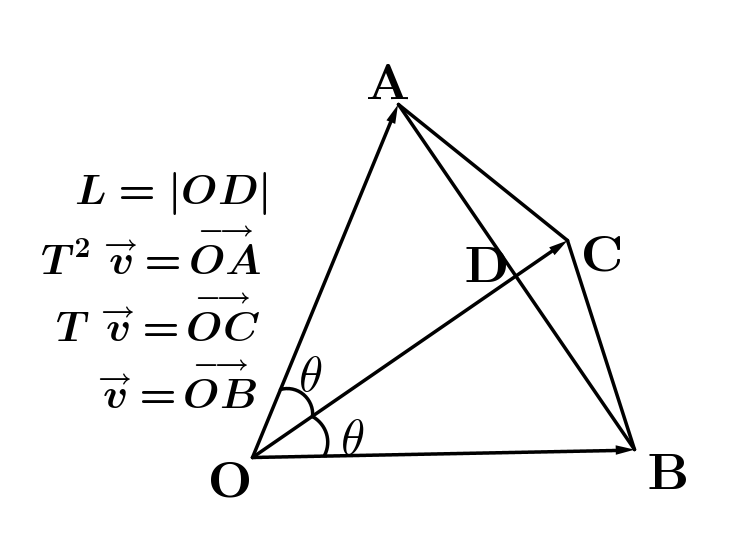
\includegraphics[scale=0.22]{./diagram.png}\par\vspace{-70pt}\quad
\hspace{180pt}{$\MathLeftMid{l}{Tv=\displaystyle\frac{\left|\overset{\rightarrow}{v}\right|}{2L}(T^2 v+v)\Rightarrow T=\frac{\left|\overset{\rightarrow}{v}\right|}{2L}(T^2+I)\\\vspace{8pt}\displaystyle L=\left|\overset{\rightarrow}{v}\right|\cos\theta\Rightarrow\frac{\left|\overset{\rightarrow}{v}\right|}{2L}=\frac{1}{2\cos\theta}}$}\par\vspace{8pt}\quad
Hence $p(T)=T^2-2\cos\theta\, T+I=0$ and $z^2-2\cos\theta\, z+1$ is the mini poly of $T.$\PfEnd\vspace{3pt}\quad
\Or By (4E 5.B.11), $\Mt(T,(e_1,e_2))=
\begin{pmatrix}
	\Blind{-}\cos\theta & \sin\theta\\
	-\sin\theta & \cos\theta
\end{pmatrix}.$\par\quad
Hence the mini poly is $z\pm 1$ or $z^2-2\cos\theta\,z+1.$\PfEnd
\SepLine

\ProblemBnoor{({\normalsize 4E 5.B.11})}{
	\TextB{Suppose $V$ is a two-dim vecsp, $T\in\Lm(V)$, and the matrix of $T$}
	\TextB{with resp to some basis of \,$V$ is {\large$\begin{pmatrix} a & c\\ b & d\end{pmatrix}.$}}
	(a) \TextB{Show that $T^2 - (a + d)T + (ad - bc)I = 0.$}
	(b) \TextB{Show that the mini poly of $T$ equals}
	\TextB{\large\centerline{$\MathLeftBrace{l}{z-a\qquad\qquad\qquad\qquad\qquad$ if $b=c=0$ and $a=d$,$\\ z^2-(a+d)z+(ad-bc)\quad$ \,\,otherwise.$}$}}
}
\par

(a) Suppose the basis is $(v,w)$. Because $\MathLeftBrace{l}{\displaystyle Tv=av+bw\Rightarrow (T-aI)v=bw,$ then apply $(T-dI)$ to both sides. $\\ Tw=cv+dw\Rightarrow (T-dI)w=cv,$ then apply $(T-aI)$ to both sides. $}$\par\vspace{6pt}\quad\Ha
Hence $(T-aI)(T-dI)=bc I\Rightarrow T^2 - (a + d)T + (ad - bc)I = 0.$\par\quad
(b) If $b=c=0$ and $a=d.$ Then $\Mt(T)=${\small$\begin{pmatrix}a & 0\\ 0 & a\end{pmatrix}$}$=a\Mt(I)$. Thus $T=aI.$ Hence the mini poly is $z-a.$\par\quad\Hb
Otherwise, by (a), $z^2-(a+d)z+(ad-bc)$ is a poly multi of the mini poly.\par\quad\Hb
Now we prove that $T\not\in\Spn(I),$ so that then the mini poly of $T$ has exactly degree $2.$\par\quad\Hb
( At least one of the assumption of (I),(II) below is true. )\par\quad\Hb
(I) Suppose $a=d,$ then $Tv=av+bw\not\in\Spn(v),Tw=cv+aw\not\in\Spn(w).$\par\qquad
(II) Suppose at most one of $b,c$ is not $0.$ If $b=0,$ then $Tw\not\in\Spn(w);$ If $c=0,$ then $Tv\not\in\Spn(v).$\PfEnd
\SepLine

\ProblemN{5}{
	\TextN{Suppose $S,T\in\Lm(V),S$ is inv, and $p\in\PoF{}$. Prove that $p(TS) = S^{-1} p(ST)S.$}
}\par\quad
We prove $(TS)^m=S^{-1}(ST)^m S$ for each $m\in\Nbb\,$ by induction.\par\quad
(i) $m=0,1.$ $TS^0=I=S^{-1}(ST)^0S;\,\,\,TS=S^{-1}(ST)S.$\par\quad\Endi
(ii) $m>1.$ Assume that $(TS)^m=S^{-1}(ST)^m S.$\par\quad\Hii\qquad\quad\hspace{-1.5pt}
Then $(TS)^{m+1}=(TS)^m(TS)=S^{-1}(ST)^m STS=S^{-1}(ST)^{m+1} S.$\par\quad
Hence $\forall p\in\PoF{},$\vspace{-23.5pt}\par\quad
\AlignEq{}{\quad p(TS)&=a_0 (TS)^0+a_1 (TS)+\dots+a_m (TS)^m\\&=a_0 [S^{-1}(ST)^0 S]+a_1 [S^{-1}(ST)S]+\dots+a_m [S^{-1}(ST)^m S]\\&=S^{-1}[a_0 (ST)^0+a_1 (ST)+\dots+a_m (ST)^m]S\\&=S^{-1}p(ST)S.}\PfEnd
\SepLine

\ProblemBnoor{({\normalsize 4E 5.B.7})\TextB{}}{
	(a) \TextB{Give an example of $S, T\in\Lm(\Fbb^2)$ such that}
	\Ha\TextB{the mini poly of
$ST$ does not equal the mini poly of $TS$.}
	(b) \TextB{Suppose $V$ is finite-dim and $S, T\in\Lm(V)$. Prove that if $S$ or $T$ is inv,}
	\Hb\TextB{then the mini poly of $ST$ equals the mini poly of $TS$.}
}\par\quad
(a) %Let $V=\Fbb^{\infty},$ $S\in\Lm(\Fbb^\infty)$ is the forward shift operator, $T\in\Lm(\Fbb^\infty)$ is the backward shift operator.\par\quad\Ha
%Then $ST(x_1,x_2,x_3,\dots)=(0,x_2,x_3,\dots)\Rightarrow 0,1$ are all the eigvals of $ST,$ $(ST)^2-(ST)=0.$\par\quad\Ha
%$TS(x_1,x_2,\dots)=(x_1,x_2,\dots)\Rightarrow 1$ is the only eigval of $TS,$ $TS=I.$\par\quad\Ha
Define $S$ by $S(x,y)=(x,x).$ Define $T$ by $T(x,y)=(0,y).$\par\quad\Ha
Then $ST(x,y)=0,\,\,TS(x,y)=(0,x)$ for all $(x,y)\in\Fbb^2.$\par\quad\Ha
Thus $ST=0\neq TS$ and $(TS)^2=0.$\par\quad\Ha
Hence the mini poly of $ST$ does not equal to the mini poly of $TS.$\par\quad
(b) Denote the mini poly of $ST$ by $p,$ and the mini poly $TS$ by $q.$\par\quad\Hb
Suppose $S$ is inv.\par\,\,\Hb
$\MathRightBrace{l}{$
$p(ST)=0=S p(TS)S^{-1}\Rightarrow p(TS)=0,p$ is a poly multi of $q.\\ $
$q(TS)=0=S^{-1} q(ST)S\Rightarrow q(ST)=0,q$ is a poly multi of $p.$
$}\Rightarrow p=q.$\par\vspace{6pt}\quad\Hb
Reversing the roles of $S$ and $T$, we conclude that if $T$ is inv, then $p=q$ as well.\PfEnd
\SepLine

\ProblemN{11}{
	\TextNL{Suppose $\Fbb = \Cbb,$ $T\in\Lm(V), p\in\PoC{}$, and $\alpha\in\Cbb.$}
	\TextNL{Prove that $\alpha$ is an eigval of $p(T)$ $\Longleftrightarrow$ $\alpha = p(\lambda)$ for some eigval $\lambda$ of $T$.}
}\par\quad
(a) Suppose $\alpha$ is an eigval of $p(T)\Leftrightarrow (p(T)-\alpha I)$ is not inje.\par\quad\Ha
Write $p(z)-\alpha=c(z-\lambda_1)\cdots(z-\lambda_m)\Rightarrow p(T)-\alpha I=c(T-\lambda_1 I)\cdots(T-\lambda_m I).$\par\quad\Ha
By \TIPS, $\,\exists\,(T-\lambda_j I)$ not inje. Thus $p(\lambda_j)-\alpha=0.$\par\quad
(b) Suppose $\alpha=p(\lambda)$ and $\lambda$ is an eigval of $T$ with an eigvec $v.$ Then $p(T)v=p(\lambda)v=\alpha v.$\PfEnd\vspace{3pt}\quad\Hb
\Or Define $q$ by $q(z)=p(z)-\alpha.$ $\lambda$ is a zero of $q.$\par\quad\Hb
Because $q(T)v=(p(T)-\alpha I)v=q(\lambda)v=(p(\lambda)-\alpha)v=0.$\par\quad\Hb
Hence $q(T)$ is not inje $\Rightarrow (p(T)-\alpha I)$ is not inje.\PfEnd
\SepLine

\ProblemN{12}{
	(\OR {\normalsize 4E.5.B.6}) \TextNL{Give an example of an operator on $\Rbb^2$}
	\TextNL{that shows the result above does not hold if $\Cbb$ is replaced with $\Rbb$.}
}\par\quad
Define $T\in\Lm(\Rbb^2)$ by $T(w,z)=(-z,w).$\par\quad
By Problem (4E 5.B.11), $\Mt\left(T,((1,0),(0,1))\right)=\,${\small$\begin{pmatrix}0 & -1\\ 1 & 0\end{pmatrix}$}$\Rightarrow$ the mini poly of $T$ is $z^2+1.$\par\quad
Define $p$ by $p(z)=z^2.$ Then $p(T)=T^2=-I.$ Thus $p(T)$ has eigval $-1.$\par\quad
While $\nexists\,\lambda\in\Rbb$ such that $-1=p(\lambda)=\lambda^2.$\PfEnd
\SepLine

\ProblemBnoor{({\normalsize4E 5.B.17})}{
	\TextB{Suppose $V$ is finite-dim, $T\in \Lm(V),\lambda\in\Fbb$, and $\,p\,$ is the mini poly of $T$.}
	\TextB{Show that the mini poly of $(T - \lambda I)$ is the poly $q$ defined by $q(z) = p(z + \lambda).$}
}\par\quad
$q(T-\lambda I)=0\Rightarrow q$ is poly multi of the mini poly of $(T-\lambda I).$\par\quad
Suppose the degree of the mini poly of $(T-\lambda I)$ is $n,$ and the degree of the mini poly of $T$ is $m.$\par\quad
%Write $q(z)=p(z+\lambda)=a_0+a_1(z+\lambda)+\dots+a_{m-1}(z+\lambda)^{m-1}+(z+\lambda)^m.$\par\quad
By definition of mini poly,\par\quad
$n$ is the smallest such that $(T-\lambda I)^n\in\Spn(I,(T-\lambda I),\dots,(T-\lambda I)^{n-1});$\par\quad
$m$ is the smallest such that $T^m\in\Spn(I,T,\dots,T^{m-1}).$\par\quad
又 $T^k\in\Spn(I,T,\dots,T^{k-1})\Longleftrightarrow (T-\lambda)^k\in\Spn(I,(T-\lambda I),\dots,(T-\lambda I)^{k-1}).$\par\quad
Thus $n=m.$ 又 $q$ is monic. By the uniqnes of mini poly.\PfEnd
\SepLine

\ProblemBnoor{({\normalsize4E 5.B.18})}{
	\TextB{Suppose $V$ is finite-dim, $T\in \Lm(V),\lambda\in\Fbb\backslash\{0\}$, and $\,p\,$ is the mini poly of $T$.}
	\TextB{Show that the mini poly of $\lambda T$ is the poly q defined by $q(z) = \lambda^{\deg p} p(\frac{z}{\lambda})$.}
}\par\quad
$q(\lambda T)=\lambda^{\deg p}p(T)=0\Rightarrow q$ is a poly multi of the mini poly of $\lambda T.$\par\quad
Suppose the degree of the mini poly of $\lambda T$ is $n,$ and the degree of the mini poly of $T$ is $m.$\par\quad
By definition of mini poly,\par\quad
$n$ is the smallest such that $(\lambda T)^n\in\Spn(\lambda I,\lambda T,\dots,(\lambda T)^{n-1});$\par\quad
$m$ is the smallest such that $T^m\in\Spn(I,T,\dots,T^{m-1}).$\par\quad
又 $(\lambda T)^k\in\Spn(\lambda I,\lambda T,\dots,(\lambda T)^{k-1})\Longleftrightarrow T^k\in\Spn(I,T\dots,T^{k-1}).$\par\quad
Thus $n=m.$ 又 $q$ is monic. By the uniqnes of mini poly.\PfEnd
\SepLine

\ProblemN{18}{
	({\normalsize \OR 4E 5.B.15}) \TextNL{Suppose $V$ is a finite-dim complex vecsp with $\dim V > 0$ and $T\in\Lm(V)$.}
	\TextNL{Define $f:\Cbb\rightarrow\Rbb$ by $f(\lambda) = \dim \range(T-\lambda I)$.}
	\TextNL{Prove that $f$ is not a continuous function.}
}Note that $V$ is finite-dim.\par\quad
Let $\lambda_0$ be an eigval of $T.$ Then $(T-\lambda_0 I)$ is not surj. Hence $\dim\range(T-\lambda_0 I)<\dim V.$\par\quad
Because $T$ has finitely many eigvals. There exist a sequence of number $\{\lambda_n\}$ such that $\lim\limits_{n\rightarrow\infty}\lambda_n=\lambda_0$.\par\quad
And $\lambda_n$ is not an eigval of $T$ for each $n\Rightarrow\dim\range(T-\lambda_n I)=\dim V\neq \dim\range(T-\lambda_0 I).$\par\quad
Thus $f(\lambda_0)\neq \lim\limits_{n\rightarrow\infty}f(\lambda_n).$\PfEnd
\SepLine

\ProblemBnoor{({\normalsize 4E 5.B.9})}{
	\TextB{Suppose $T\in\Lm(V)$ is such that with resp to some basis of \,$V$,}
	\TextB{all entries of the matrix of $T$ are rational numbers.}
	\TextB{Explain why all coefficients of the mini poly of $T$ are rational numbers.}
}\par\quad
Let $(v_1,\dots,v_n)$ denote the basis such that $\Mt\left(T,(v_1,\dots,v_n)\right)_{j,k}=A_{j,k}\in\Qbb$ for all $j,k=1,\dots,n$.\par\quad
Denote $\Mt\left(v_j,(v_1,\dots,v_n)\right)$ by $x_j$ for each $v_j.$\par\quad
Suppose $p$ is the mini poly of $T$ and $p(z)=z^m+\dots+c_1 z+c_0.$ Now we show that each $c_j\in\Qbb.$\par\quad
Note that $\forall s\in\Nbp,\Mt(T^s)=\Mt(T)^s=A^s\in\Qbb^{n,n}$ and $T^s v_k=A^s_{1,k} v_1+\dots+A^s_{n,k}v_n$ for all $k\in\{1,\dots,n\}.$\par\vspace{6pt}\quad
Thus $\MathLeftBrace{l}{
\Mt(p(T)v_1)=(A^m+\dots+c_1 A+c_0 I)x_1=\sum\limits_{j=1}^n(A^m+\dots+c_1 A+c_0 I)_{j,1}x_j=0;\\ \qquad\qquad\vdots \\
\Mt(p(T)v_n)=(A^m+\dots+c_1 A+c_0 I)x_n=\sum\limits_{j=1}^n(A^m+\dots+c_1 A+c_0 I)_{j,n}x_j=0;
}$\par\quad
More clearly, $\MathLeftBrace{l}{
(A^m+\dots+c_1 A+c_0 I)_{1,1}=\cdots=(A^m+\dots+c_1 A+c_0 I)_{n,1}=0;\\\hspace{130pt}\vdots\hspace{8pt}\ddots\hspace{8pt}\vdots\\
(A^m+\dots+c_1 A+c_0 I)_{1,n}=\cdots=(A^m+\dots+c_1 A+c_0 I)_{n,n}=0;
}$\par\quad
Hence we get a system of $n^2$ linear equations in $m$ unknowns $c_0,c_1,\dots,c_{m-1}.$\par\quad
We conclude that $c_0,c_1,\dots,c_{m-1}\in\Qbb.$\PfEnd
\SepLine

\ProblemBnoor{{\normalsize \OR (4E 5.B.16), \OR (8.C.18})}{
	\TextB{Suppose $a_0 ,\dots, a_{n-1}\in\Fbb.$ Let $T$ be the operator on $\Fbb^n$ such that\vspace{2pt}}
	\TextB{$\Mt(T)=\,${\normalsize$\begin{pmatrix}
	0 &   &        &  &   & -a_0     \\
	1 & 0 &        &  &   & -a_1     \\
	  & 1 & \ddots &  &   & \vdots   \\
	  &   & \ddots &  & 0 & -a_{n-2} \\
	0 &   &        &  & 1 & -a_{n-1}
\end{pmatrix} $}, with resp to the standard basis $(e_1,\dots,e_n)$.\vspace{4pt}}
	\TextB{Show that the mini poly of $T$ is $\,p\,$ defined by $p(z)=a_0 + a_1 z + \dots + a_{n-1} z^{n-1} + z^n$.}
	\vspace{-2pt}\TextB{\small $\Mt(T)$ is called the {\tgsc companion matrix} of the poly above. This exercise shows that every monic poly is the mini poly of some operator.}
	\vspace{-2pt}\TextB{\small Hence a formula or an algorithm that could produce exact eigvals for each operator on each $\Fbb^n$ could then produce exact zeros for}
	\vspace{-2pt}\TextB{\small each poly  $[$ by 8.36(b) $]$. Thus there is no such formula or algorithm. However, efficient numeric methods exist for obtaining very good}
	\TextB{\small approximations for the eigvals of an operator.}
}Note that $(e_1,Te_1,\dots,T^{n-1}e_1)$ is linely inde. 又 The deg of mini poly is at most $n.$\par\quad
$T^n e_1=\cdots=T^{n-k}e_{1+k}=\cdots=T e_n=-a_0 e_1-a_1 e_2-a_2 e_3-\dots-a_{n-1}e_n$\par
$=(-a_0 I-a_1 T-a_2 T^2-\dots-a_{n-1}T^{n-1})e_1.$ Thus $p(T)e_1=0=p(T)e_j$ for each $e_j=T^{j-1}e_1.$\PfEnd
\SepLine

\BulletPoint \,\hspace{1pt}{\Large\textsc{Eigenvalues On Odd-Dimensional Real Vector Spaces}}\par
\ProblemB{
	\textsc{Even-Dimensional Null Space}\TextB{}
	\TextB{Suppose $\Fbb=\Rbb,$ $V$ is finite-dim, $T\in\Lm(V)$ and $b, c\in\Rbb$ with $b^2 < 4c$.}
	\TextB{Prove that $\dim\null(T^2 + bT + cI)$ is an even number.}
}\par\quad
Denote $\null(T^2 + bT + cI)$ by $R.$ Then $T|_R+bT|_R+cI_R=(T+bT+cI)|_R=0\in\Lm(R).$\par\quad
Suppose $\lambda$ is an eigval of $T_R$ with an eigvec $v\in R.$\par\quad
Then $\displaystyle 0=(T|_R^2+bT|_R+cI_R)(v)=(\lambda^2+\lambda b+c)v=\left((\lambda+b)^2+c-\frac{b^2}{4}\right)v.$\par\quad
Because $\displaystyle c-\frac{b^2}{4}>0$ and we have $v=0.$ Thus $T_R$ has no eigvals.\par\quad
Let $U$ be an invar subsp of $R$ that has the largest, even dim among all invar subsps.\par\quad
Assume that $U\neq R.$ Then $\,\exists\,w\in R$ but $w\not\in U.$ Let $W$ be such that $(w,T|_R w)$ is a basis of $W.$\par\quad
Because $T|_R^2 w=-bT|_R w-cw\in W.$ Hence $W$ is an invar subsp of dim $2.$\par\quad
Thus $\dim (U+W)=\dim U+2-\dim(U\cap W),$ where $U\cap W=\{0\},$\par\qquad\qquad
for if not, because $w\not\in U,T|_R w\in U,$\par\qquad\qquad $U\cap W$ is invar under $T|_R$ of one dim ( impossible because $T|_R$ has no eigvecs ).\par\quad
Hence $U+W$ is even-dim invar subsp under $T|_R$, contradicting the maximality of $\dim U.$\par\quad
Thus the assumption was incorrect. Hence $R=\null(T^2+bT+cI)=U$ has even dim.\PfEnd
\SepLine

\ProblemB{
	\textsc{Operators On Odd-Dimensional Vector Spaces Have Eigenvalues}\TextB{}
	(a) \TextB{Suppose $\Fbb=\Cbb.$ \tgnr\large Then by [5.21], we are done.}
	(b) \TextB{Suppose $\Fbb=\Rbb,$ $V$ is finite-dim, and $\dim V=n$ is an odd number.}
	\Hb\TextB{Let $T\in\Lm(V)$ and the mini poly is $\,p\,$. Prove that $T$ has an eigval.}
}\par\quad
(i) If $n=1,$ then we are done.\par\quad\Endi
(ii) Suppose $n\geq 3.$ Assume that every operator, on odd-dim vecsps of dim less than $n,$ has an eigval.\par\quad\Hii
If $p$ is a poly multi of $(x - \lambda)$ for some $\lambda\in\Rbb,$ then by [8.49] $\lambda$ is an eigval of $T$ and we are done.\par\quad\Hii
Now suppose $b, c\in\Rbb$ such that $b^2 < 4c$ and $p$ is a poly multi of $x^2 + bx + c$ (see [4.17]).\par\quad\Hii
Then $\,\exists\,q\in\PoR{}$ such that $p(x) = q(x)(x^2 + bx + c)$ for all $x\in\Rbb.$\par\quad\Hii
Now $0 = p(T) = \left(q(T)\right)(T^2 + bT + cI),$ which means that $q(T)|_{\range(T^2+bT+cI)}=0.$\par\quad\Hii
Because $\deg q < \deg p$ and $p$ is the mini poly of $T$, hence $\range(T^2 + bT + cI)\neq V$.\par\quad\Hii
又 $\dim V$ is odd and $\dim\null(T^2 +bT+cI)$ is even ( by our previous result ).\par\quad\Hii
Thus $\dim V - \dim \null(T^2 + bT + cI)=\dim \range(T^2 + bT + cI)$ is odd.\par\quad\Hii
By [5.18], $\range(T^2 + bT + cI)$ is an invar subsp of $V$ under $T$ that has odd dim less than $n.$\par\quad\Hii
Our induction hypothesis now implies that $T|_{\range(T^2 + bT + cI)}$ has an eigval.\par\quad
By mathematical induction.\PfEnd
\SepLine

\ProblemBnoor{({\normalsize 2E Ch5.24})}{
	\TextB{Suppose $\Fbb=\Rbb,T\in\Lm(V)$ has no eigvals.} \TextB{Prove that every invar subsp of \,$V$ under $T$ is even-dim.}
}\par\quad
Suppose $U$ is such a subsp. Then $T|_U\in\Lm(U).$
We prove by contradiction.\par\quad
If $\dim U$ is odd, then $T|_U$ has an eigval and so is $T,$ so that $\,\exists$ invar subsp of $1$ dim, contradicts.\PfEnd
\SepLine

\ProblemBnoor{({\normalsize4E 5.B.29})}{
	\TextB{Show that every operator on a finite-dim vecsp of dim $\geq 2$ has a $2$-dim invar subsp.}
}\par\quad
Using induction on $\dim V.$\par\quad
(i) $\dim V=2,$ we are done.\par\quad\Endi
(ii) $\dim V>2.$ Assume that the desired result is true for vecsp of smaller dim.\par\quad\Hii
Suppose $p$ is the mini poly of degree $m$ and $p(z)=(z-\lambda_1)\cdots(z-\lambda_m).$\par\quad\Hii
If $\,T=\lambda I\,(\,\Leftrightarrow m=1\,\vee\,m=-\infty\,),$ then we are done. ( $m\neq 0$ because $\dim V\neq 0.$ )\par\quad\Hii
Now define a $q$ by $q(z)=(z-\lambda_1)(z-\lambda_2)$.\par\quad\Hii
By assumption, $T|_{\null q(T)}$ has an invar subsp of dim $2.$\PfEnd
\SepLine

\ChEnd

% 6h
\ChDecl{Ch5BII}{5.B: II}


\ProblemBnoor{({\normalsize4E 5.C.1})}{
	\TextB{Prove or give a counterexample:}
	\TextB{If $T\in \Lm(V)$ and $T^2$ has an upper-trig matrix, then $T$ has an upper-trig matrix.}
}\par
\SepLine

\ProblemBnoor{({\normalsize4E 5.C.2})}{
	\TextB{Suppose $A$ and $B$ are upper-trig matrices of the same size,}
	\TextB{with $\alpha_1 , \dots , \alpha_n$ on the diag of $A$ and $\beta_1 , \dots , \beta_n$ on the diag of $B$.}
	(a) \TextB{Show that $A + B$ is an upper-trig matrix with $\alpha_1 + \beta_1 , \dots , \alpha_n + \beta_n$ on the diag.}
	(b) \TextB{Show that $AB$ is an upper-trig matrix with $\alpha_1 \beta_1 , \dots , \alpha_n \beta_n$ on the diag.}
}\par
\SepLine

\ProblemBnoor{({\normalsize4E 5.C.3})\TextB{}}{
	\TextB{Suppose $T\in \Lm(V)$ is inv and $B=(v_1 , \dots , v_n)$ is a basis of \,$V$ such that}
	\TextB{$\Mt(T,B)=A$ is upper trig, with $\lambda_1 , \dots , \lambda_n$ on the diag.}
	\TextB{Show that the matrix of $\Mt(T^{-1},B)=A^{-1}$ is also upper trig, with
{\normalsize$\displaystyle\frac{1}{\lambda_1},\dots,\frac{1}{\lambda_n}$} on the diag.}
}\par
\SepLine

\ProblemN{9}{
	({\normalsize4E 5.C.7})\TextN{}
	\TextN{Suppose $V$ is finite-dim, $T\in \Lm(V)$, and $v \in V$.}
	(a) \TextN{Prove that $\,\exists\,!$ monic poly $p_v$ of smallest degree such that $p_v (T)v = 0$.}
	(b) \TextN{Prove that the mini poly of $T$ is a poly multi of $p_v$.}
}\par
\SepLine


\ProblemN{14}{
	({\normalsize \OR 4E 5.C.4})\TextNL{ Give an operator $T$ such that with resp to some basis,}
	\TextNL{$\Mt(T)_{k,k}=0$ for each $k$, while $T$ is inv.}
}
\par
\SepLine

\ProblemN{15}{
	({\normalsize \OR 4E 5.C.5})\TextNL{ Give an operator $T$ such that with resp to some basis,}
	\TextNL{$\Mt(T)_{k,k}\neq 0$ for each $k$, while $T$ is not inv.}
}\par


\par
\SepLine

\ProblemN{20}{
	({\normalsize \OR 4E 5.C.6})\TextNL{}
	\TextNL{Suppose $\Fbb=\Cbb,$ $V$ is finite-dim, and $T\in\Lm(V)$.}
	\TextNL{Prove that if $k\in\{1,\dots,\dim V\},$ then \,$V$ has a $k$ dim subsp invar under $T$.}
}\par
\SepLine

\ProblemBnoor{({\normalsize 4E 5.C.8})}{
	\TextB{Suppose $V$ is finite-dim, $T\in \Lm(V)$, and $\,\exists\,v \in V\backslash\{0\}$ such that $T^2 v + 2Tv = -2v$.}
	(a) \TextB{Prove that if $\Fbb=\Rbb,$ then $\nexists$ a basis of \,$V$ with resp to which $T$ has an upper-trig matrix.}
	(b) \TextB{Prove that if $\Fbb=\Cbb$ and $A$ is an upper-trig matrix that equals the matrix of $T$}
	\Hb\TextB{with resp to some basis of \,$V$, then $-1 + \i$ or $-1 - \i$ appears on the diag of $A$.}
}\par
\SepLine

\ProblemBnoor{({\normalsize 4E 5.C.9})}{
	\TextB{Suppose $B\in\Fbb^{n,n}$ with complex entries.}
	\TextB{Prove that $\,\exists$ inv $A\in\Fbb^{n,n}$ with complex entries such that $A^{-1} BA$ is an upper-trig matrix.}
}\par

\par
\SepLine

\ProblemBnoor{({\normalsize 4E 5.C.10})}{
	\TextB{Suppose $T\in \Lm(V)$ and $(v_1,\dots,v_n)$ is a basis of \,$V$.}
	\TextB{Show that the following are equi.}
	(a) \TextB{The matrix of $T$ with resp to $(v_1,\dots,v_n)$ is lower trig.}
	(b) \TextB{$\Spn(v_k,\dots,v_n)$ is invar under $T$ for each $k=1,\dots,n$.}
	(c) \TextB{$Tv_k\in\Spn(v_k,\dots,v_n )$ for each $k=1,\dots,n$.}
}\par
\SepLine

\ProblemBnoor{({\normalsize 4E 5.C.11})}{
	\TextB{Suppose $\Fbb=\Cbb$ and $V$ is finite-dim.}
	\TextB{Prove that if $T\in \Lm(V)$, then $T$ has a lower-trig matrix with resp to some basis.}
}\par
\SepLine

\ProblemBnoor{({\normalsize 4E 5.C.12})\TextB{}}{
	\TextB{Suppose $V$ is finite-dim, $T\in \Lm(V)$ has an upper-trig matrix with resp to some basis,}
	\TextB{and $U$ is a subsp of \,$V$ that is invar under $T$.}
	(a) \TextB{Prove that $T|_U$ has an upper-trig matrix with resp to some basis of $U$.}
	(b) \TextB{Prove that $T/U$ has an upper-trig matrix with resp to some basis of \,$V/U$.}
}\par


\par
\SepLine

\ProblemBnoor{({\normalsize 4E 5.C.13})}{
	\TextB{Suppose $V$ is finite-dim, $T\in \Lm(V)$. Suppose $U$ is an invar subsp of \,$V$ under $T$}
	\TextB{such that $T|_U$ has an upper-trig matrix and also $T/U$ has an upper-trig matrix.}
	\TextB{Prove that $T$ has an upper-trig matrix.}
}\par


\par
\SepLine

\ProblemBnoor{({\normalsize 4E 5.C.14})}{
	\TextB{Suppose $V$ is finite-dim and $T\in \Lm(V)$.}
	\TextB{Prove that $T$ has an upper-trig matrix $\Longleftrightarrow$ $T\apostrophe$ has an upper-trig matrix.}
}\par


\par
\SepLine

\ChEnd

\ChDecl{Ch5C}{5.C} % 10h

XXXX


\par
\SepLine

\ChEnd
\ChDecl{Ch5E}{5.E* (4E)} % 0.5h/4h

\ProblemN{1}{
	\TextN{Give an example of two commuting operators $S, T\in\Fbb^4$ such that}
	\TextN{there is an invar subsp of $\Fbb^4$ under $S$ but not under $T$}
	\TextN{and an invar subsp of $\Fbb^4$ under $T$ but not under $S$.}
}
\par
\SepLine

\ProblemN{2}{
	\TextN{Suppose $\mathcal{E}$ is a subset of $\Lm(V)$ and every element of $\mathcal{E}$ is diagable.}
	\TextN{Prove that $\,\exists$ a basis of \,$V$ with resp to which}
	\TextN{every element of $\mathcal{E}$ has a diag matrix $\Longleftrightarrow$ every pair of elements of $\mathcal{E}$ commutes.}
	\TextN{{\normalsize This exercise extends [5.76], which considers the case in which $\mathcal{E}$ contains only two elements.}}\hspace{0.5pt}
	\TextN{{\normalsize For this exercise, $\mathcal{E}$ may contain any number of elements, and $\mathcal{E}$ may even be an infinite set.}}
}\par
\SepLine

\ProblemN{3}{
	\TextN{Suppose $S, T\in\Lm(V)$ are such that $ST = TS$. Suppose $p\in\PoF{}$.}
	(a) \TextN{Prove that $\null p(S)$ is invar under $T$.}
	(b) \TextN{Prove that $\range p(S)$ is invar under $T$.}
	\TextN{See \NOTEFOR [5.17] for the special case $S = T$.}
}\par
\SepLine

\ProblemN{4}{
	\TextN{Prove or give a counterexample:}
	\TextN{A diag matrix $A$ and an upper-trig matrix $B$ of the same size commute.}
}\par
\SepLine

\ProblemN{5}{
	\TextN{Prove that a pair of operators on a finite-dim vecsp commute $\Longleftrightarrow$ their dual operators commute.}
}\par
\SepLine

\ProblemN{6}{
	\TextN{Suppose $V$ is a finite-dim complex vecsp and $S, T\in\Lm(V)$ commute.}
	\TextN{Prove that $\,\exists\,\alpha,\lambda\in\Cbb$ such that $\range(S -\alpha I) + \range(T -\lambda I)\neq V$.}
}\par
\SepLine

\ProblemN{7}{
	\TextN{Suppose $V$ is a complex vecsp, $S\in\Lm(V)$ is diagable, and $T$ commutes with $S$.}
	\TextN{Prove that $\,\exists$ basis $B$ of $V$ such that $S$ has a diag matrix with resp to $B$}
	\TextN{and T has an upper-trig matrix with resp to $B$.}
}\par
\SepLine

\ProblemN{8}{
	\TextN{Suppose $m = 3$ in Example [5.72]}
	\TextN{and $D_x , D_y$ are the commuting partial differentiation operators on $\Po_3(\Rbb^2)$ from that example.}
	\TextN{Find a basis of $\Po_3(\Rbb^2)$ with resp to which $D_x$ and $D_y$ each have an upper-trig matrix.}
}\par
\SepLine

\ProblemN{9}{
	\TextN{Suppose $V$ is a finite-dim nonzero complex vecsp.}
	\TextN{Suppose that $\mathcal{E}\subseteq\Lm(V)$ is such that $S$ and $T$ commute for all $S, T\in\mathcal{E}$.}
	(a) \TextN{Prove that $\,\exists\,v\in V$ is an eigvec for every element of $\mathcal{E}$.}
	(b) \TextN{Prove that $\,\exists$ a basis of \,$V$ with resp to which every element of $\mathcal{E}$ has an upper-trig matrix.}
}\par
\SepLine

\ProblemN{10}{
	\TextNL{Give an example of two commuting operators $S, T$ on a finite-dim real vecsp such that}
	\TextNL{$S + T$ has a eigval that does not equal an eigval of $S$ plus an eigval of $T$}
	\TextNL{and $ST$ has a eigval that does not equal an eigval of $S$ times an eigval of $T$.}
}
\par
\SepLine
\ChEnd

\end{large}
\end{document}
